% Dissertation
% 06/28/2013
% (Use \include{filename} in diss file

\documentclass[12pt]{report} 	% report used for dissertations

\usepackage{anysize} 		% allows me to set margins
\usepackage{indentfirst}
\usepackage{apacite}		% for apa style
\usepackage{graphicx}		% for graphics
\usepackage{times}
\usepackage{mathtools}
\usepackage{textcomp}
\usepackage{amsmath}
\usepackage{afterpage}
\usepackage{setspace}
\usepackage{titlesec}
\usepackage[normalem]{ulem}

\titleformat{\chapter}[display]
  {\normalfont\fontfamily{ptm}\fontsize{14}{17}\selectfont\filcenter}{CHAPTER \thechapter}{0pt}{}
  \titlespacing*{\chapter}
  {0pt}{28pt}{40pt}
\titleformat{\section}
  {\normalfont\fontfamily{ptm}\fontsize{14}{17}\selectfont}{\thesubsection}{1em}{\uline}
\titleformat{\subsection}
  {\normalfont\fontfamily{ptm}\fontsize{14}{17}\selectfont\filcenter}{\thesubsubsection}{1em}{\uline}
 \titleformat{\subsubsection}
  {\normalfont\fontfamily{ptm}\fontsize{14}{17}\selectfont}{\thesubsubsection}{1em}{}

\numberwithin{figure}{chapter}
\numberwithin{table}{chapter}
\numberwithin{equation}{chapter}

\usepackage{chngcntr}
\counterwithout{figure}{chapter}
\counterwithout{table}{chapter}
\counterwithout{equation}{chapter}

\renewcommand\thechapter{\Roman{chapter}}

%\marginsize{1.5in}{1.5in}{1.25in}{1.25in}	% left, right, top, bottom
\usepackage[paperwidth=8.5in, paperheight=11in]{geometry}
\geometry{top = 1.25in, left = 1.5in, right = 1.5in, bottom=1.25in, footskip=0.5in}
\begin{document}

\begin{titlepage}
\begin{center}
\begin{tabular}{llll}
  Sponsoring Committee: & Professor Robert Rowe\\
  & Professor Juan P. Bello\\
  & Professor R. Luke Dubois\\
\end{tabular}
\\
\vfill
EVOLVING SYNTHESIS ALGORITHMS USING A MEASURE\\
\vspace{\baselineskip}
OF TIMBRAL SEQUENCE SIMILARITY\\
\vspace{\baselineskip}
\vspace{\baselineskip}
\vspace{\baselineskip}
Aron Glennon\\
\vspace{\baselineskip}
Program in Music Technology\\
Department of Music and Performing Arts Professions\\
\vfill
Submitted in partial fulfillment\\
of the requirements for the degree of\\
Doctor of Philosophy in the\\
Steinhardt School of Culture, Education, and Humanities Development\\
New York University\\
2014\\
\end{center}
\end{titlepage}
\begin{flushleft}				% generates left-aligned paragraphs
\setlength{\parindent}{30pt}	% This starts every paragraph with an indent

\begin{copyrightpage}
\thispagestyle{empty}
\topskip0pt
\vspace*{\fill}
\begin{center}
Copyright \copyright{} 2014 Aron Glennon
\end{center}
\vspace*{\fill}
\end{copyrightpage}
\clearpage
\pagenumbering{roman}			% roman numbering until introduction	
\doublespacing

% Acknowledgements
\renewcommand\abstractname{\normalfont \large ACKNOWLEDGEMENTS}
\newgeometry{top = 2.0in}
\doublespacing
\thispagestyle{plain}
\setcounter{page}{3}
\addcontentsline{toc}{subsection}{ACKNOWLEDGEMENTS}
\begingroup
\begin{center}
    \fontsize{14pt}{17pt}\selectfont
    ACKNOWLEDGEMENTS
\end{center}
\endgroup
\hspace*{\parindent}This work could not have been completed without the patience and support of many different individuals. I would like to specifically thank:

My advisor Prof. Robert Rowe for providing me with the appropriate amount of freedom to follow my instincts when they were strong and the appropriate amount of guidance when I led myself to forks in the road.

My adopted advisor (though I'm not sure who adopted who) Prof. Juan Bello for always pushing me to do more, for always being there to talk through even the most wild ideas, and for nurturing my interest in both Music Information Retrieval and Machine Learning. While I always looked to Juan for advice and viewed him as a mentor, I always felt that he was more of a friend than anything.

Adam Rokhsar for the almost-daily conversations about what I was really after and why I had chosen to pursue it via academia, and for the constant reminders (sometimes verbal, sometimes through collaboration) that I am first and foremost a composer.

Kyle Needham and Ryan Glennon for cultivating my interest in music in the first place. Whenever I hear something new that I think will change the world, I always wonder what you both would think of it.

My peers in the NYU Music Technology doctoral program, but specifically Jon Forsyth and Eric Humphrey: Jon, for all of the conversations we had that had nothing to do with the PhD process, Music Tech, MIR, or Machine Learning; Eric, for all of the conversations that did.

Bill Lord, Mason Smith, Michael Cagliuso, David Leveroni, Mariel Matero, and Andy Melnyk: Without the parts of my life that made me feel like a normal human being, \newgeometry{top = 1.25in}\doublespacing
\setlength{\parindent}{0pt}	% This starts every paragraph with an indent
I couldn't have completed a task that feels so not-normal.
\setlength{\parindent}{30pt}	% This starts every paragraph with an indent

My former DST students: Thank you for convincing me that academia is where I ultimately belong.

My parents, parents-in-law, sisters- and brother-in-law, and the rest of my friends and family for always reminding me of what matters most in life.

Most importantly, my wife Lauren, and my children Henry, Jack, and Charles. I could write ten dissertations and still not be able to fully explore the complexity nor explain the true gravity of my love for you.
\clearpage
% In Memory of
\begin{center}
\vspace*{\fill}
In memory of Marguerite Danico (1926-2009)\\ and Bruce Singleton (1971-2011)
\vspace*{\fill}
\end{center}

\singlespacing

\setcounter{tocdepth}{4}			% subsubsection in toc
\setcounter{secnumdepth}{0}	% level of sections that are numbered

\selectfont			
\setcounter{page}{5}
% list doc, figures, tables
\titleformat{\chapter}[display]

\renewcommand\contentsname{TABLE OF CONTENTS}
\tableofcontents

\doublespacing

\setcounter{page}{8}

\renewcommand*\listtablename{LIST OF TABLES}
\addcontentsline{toc}{subsection}{LIST OF TABLES}
\listoftables

\cleardoublepage
\renewcommand*\listfigurename{LIST OF FIGURES}
\addcontentsline{toc}{subsection}{LIST OF FIGURES} 
\listoffigures

% we define QuarterPage for the beginning of all chapters
\newlength{\QuarterPage}
\setlength{\QuarterPage}{1.0in}
				
\vspace*{\QuarterPage}
\newpage
\pagenumbering{arabic}
\chapter{INTRODUCTION} % * suppresses heading numbers	
Timbre has played an increasingly important role in music composition since the beginning of the 20th century. With the advent of digital technology, composers have been given the power to generate sounds with boundless timbral variation. However, true timbral exploration is still out of reach for all but the the most technically inclined and dedicated, as the mechanisms that provide timbral control (synthesis algorithms) are often non-intuitive unless one has a strong understanding of the mathematics that underlie their sound production; and even in this case, achieving a desired timbre often requires a large amount of trial-and-error. To further complicate things, a variety of synthesis algorithms exist, each suited to produce only a subset of all possible timbres. Therefore, in order to successfully generate a desired timbre (or explore a specific region of timbre space) one must first choose an appropriate synthesis algorithm and then find a suitable parameter set for the chosen topology. Placing this burden on the composer requires them to spend more time on trial-and-error searching and less time composing. The less technically inclined the composer is, the more time they will likely spend performing tasks that are not beneficial to their compositional process. It is our goal to shorten this search process for all composers, removing the inherent bias towards the mathematically sophisticated.

Approaching timbre matching through the lens of automatic programming, we have developed a system intended to automate this search process to discover a synthesis topology well suited to the desired timbre, while simultaneously finding an appropriate parameter set that realizes it. More formally, this system performs an intelligently directed search through the space of all possible synthesis topologies and parameter sets in order to find a proper algorithm to produce a user-supplied desired timbre.

We approached this research with the following goals:
\begin{enumerate}
\item To determine an appropriate environment within which to automatically generate synthesis topologies and to establish a suitable topology representation that defines a space over which we will search.
\item To decide upon a well-suited intelligent search algorithm for navigating the space of synthesis topologies defined by subproblem 1 and to find the best architecture for that algorithm.
\item To find ways of restricting the search space and making the search algorithm most efficient and powerful without omitting optimal solutions.
\item To decide upon an objective timbre representation in which distances are semantically meaningful, information regarding the temporal evolution of timbre is retained, and whose elements are invariant to changes in pitch and loudness.
\item To develop an appropriate similarity metric, over trajectories in the objective timbre space chosen in subproblem 4, that will be appropriate for comparing time-varying timbral content. This metric will help define an objective landscape over synthesis algorithm space whose global optimum will correspond to the desired solution.
\item To combine the solutions of the above subproblems into a system implementation capable of automatically generating synthesis algorithms that not only match the target timbre, but that also exhibit attractive properties for synthesis algorithms in general.
\end{enumerate}

\section{Motivations}
This study attempts to develop a system that, given a desired location in timbre space, is able to construct a synthesis algorithm with a low-dimensional parameter set, low time-complexity, and low space-complexity that maps to that location. By intelligently choosing which algorithm and parameter mapping to use for a given region of timbre space, this system will act as a meta-synthesizer able to automatically construct efficient synthesis topologies for any timbral region.

This research has the potential to impact a number of areas of study including computer music, music information retrieval, artificial intelligence (of which automatic programming research is a subset), and signal processing.

Practically speaking, the proposed system will extend the sonic palette of any composer (or producer) utilizing digital audio effects or synthesis algorithms regularly in their works. The availability of a larger timbral tool set for these composers will naturally lead to more experimentation and timbral exploration as composers will be able to create with timbre in ways previously not available to them. Placing the burden of timbral search on the computer would also free up more time to compose, likely leading to increased compositional output: a benefit to the music community as a whole.

In constructing this system, we investigate more appropriate ways of measuring local timbral similarity than are currently available in the literature. Local timbral sequence similarity is a far less researched topic than global timbral similarity in the MIR community. However, we believe that much can be learned about timbre on a local time scale, especially in cases where its specific temporal evolution contributes greatly to its perception. Also, by investigating timbral similarity over sequences of vectors within state-of-the-art objective timbre spaces (whose distance measurements are semantically meaningful), this research will benefit MIR researchers interested in, for example, instrument classification, song similarity, audio fingerprinting, and vocalist recognition.

This study will also contribute to the growing body of research targeted toward the use of artificial intelligence in artistic applications. Most research in this area deals with the creation of artistic works by machines and there is much less work focused on using artificial intelligence to generate new tools for human creators interested in a more traditional creation process. This research hopes to change that trend by exemplifying the importance of tool generation for artists that are not satisfied with their present means of creation. Specifically, within the domain of artificial intelligence, almost all practical automatic programming research targets designing software for solving scientific problems (e.g. robot mechanics, circuit board design). Therefore, this study, drawing primarily from the automatic programming research community, integrates a domain typically interested in solving scientific problems with one of artistic creation in a way not yet approached rigorously.

In summary, this study is significant from both theoretical and practical perspectives and contributes to a number of different disciplines ranging from applied computer science and digital signal processing to computer music composition, music production, and music information retrieval.
\vspace{12pt}
\section{Overview}
The system proposed in this study is based on a large body of research in timbre, timbral similarity, sequence similarity, and automatic programming. The necessary background, ideas developed around it, and exploration of these ideas are presented as follows:

Chapter II provides an overview of the prior work leveraged in this study. Beginning with a basic treatment of the complexities involved in defining \textit{timbre}, it moves on to enumerate the various kinds of sound synthesis algorithms in common use in computer music and discusses the difficulty of estimating appropriate parameters for a specific algorithm given a desired timbre. Various re-synthesis algorithms are presented as solutions to this problem, leading into a discussion of meta-synthesis and its advantages over re-synthesis. The chapter ends with an overview of state-of-the-art meta-synthesis research and focuses on advancements related to the use of intelligent search algorithms to find optimal synthesis topologies and parameterizations.

Chapter III focuses on our approach to advancing research in meta-synthesis. It begins with a discussion of our synthesis topology representation (both in theory and in implementation) and how this representation fits within the standard automatic programming framework. The chapter then covers our design of an appropriate timbral sequence similarity measure. Finally, the chapter ends with a discussion of the ways in which we refine the standard automatic programming search process.

Chapter IV covers the design of the assorted experiments performed to optimize the different pieces of the search algorithm, providing both a rationale for the variants of each module tested and the order in which the experiments are executed.

Chapter V presents and analyzes the results of all experiments discussed in Chapter IV.

Chapter VI provides conclusions based on the results found in Chapter V, notes limitations experienced throughout testing and what effects they may have had on these results, and suggests possible areas of future work.

\vspace*{\QuarterPage}
\chapter{PRIOR WORK} % * suppresses heading numbers
The development of a system capable of matching user-provided timbres benefits from a large body of literature and would not be possible without the work of a number of very talented researchers. This chapter endeavors to cover the most critical research pertaining to this study. This involves investigations into (the mostly opaque) definitions of timbre, the history, evolution, and qualities of sound synthesis algorithms, and the problem of timbre matching using both fixed sound synthesis topologies and those that are allowed to vary.
\vspace{12pt}
\section{Timbre}
While timbre is a term in common use within the music community, its precise definition has remained elusive. In his thesis on tracking timbre, Shiraishi notes this is in \begin{singlespace}\noindent part because:
%\linespread{1}
\selectfont
\begin{quote}
The term \textit{timbre} itself is often confused with two different distinctions. On one hand, we recognize that different acoustic instruments have timbre. The piano has timbre of the piano...for instance. On the other hand, one instrument can be played with a performer's delicate timbre manipulation \cite[p. 4]{Shiraishi:2006ye}.
\end{quote}
\end{singlespace}
%\linespread{1.7}
\selectfont
In other words, one can associate a single timbre to a single sound-producing body or to a single sonic \textit{character} possibly attainable by many different sound-producing bodies. Nicol writes that ``ecological listening states that humans are more likely to describe sounds with reference to the apparent source of that sound as opposed to certain characteristics of that sound'' implying that the former association with timbre may be more often valid \cite[p. 23]{Nicol:2005rp}. However, for this research the latter association is more relevant and will be adopted going forward. 

Johnson and Gounaropoulos make a separate distinction between two different types of timbre that are also often confused, differing in time scale \cite{Johnson:2006pi}. They write, in their study on associating words with timbral features extracted from an audio signal, that ``by timbre we will mean the micro-level spectral characteristics of sound as discussed by Wishart, as opposed to the gross timbral distinctions used e.g. in the MPEG-7 standard'' \cite[p. 1]{Johnson:2006pi}. This refers to a confusion between local versus global timbral representations. We find the former of these two most relevant to this research and also adopt this going forward.

It is clear from the above examples that the many different interpretations of the word \textit{timbre} make it a relatively opaque concept. Stowell and Plumbley note that ``evidence from perceptual studies tells us that timbre is multidimensional and probably non-linear'' \cite[p. 1]{Stowell:2008qf}. Aside from this, the results of this research often conflict, most likely due to the ambiguity associated with the term \cite[p. 4]{Fiebrink:os}, \cite[p. 11]{Ciglar:2009uf}.

There are two approaches to defining timbre (see Figure 1): an additive definition and a subtractive one. 
\begin{figure}[!htp]
\begin{center}
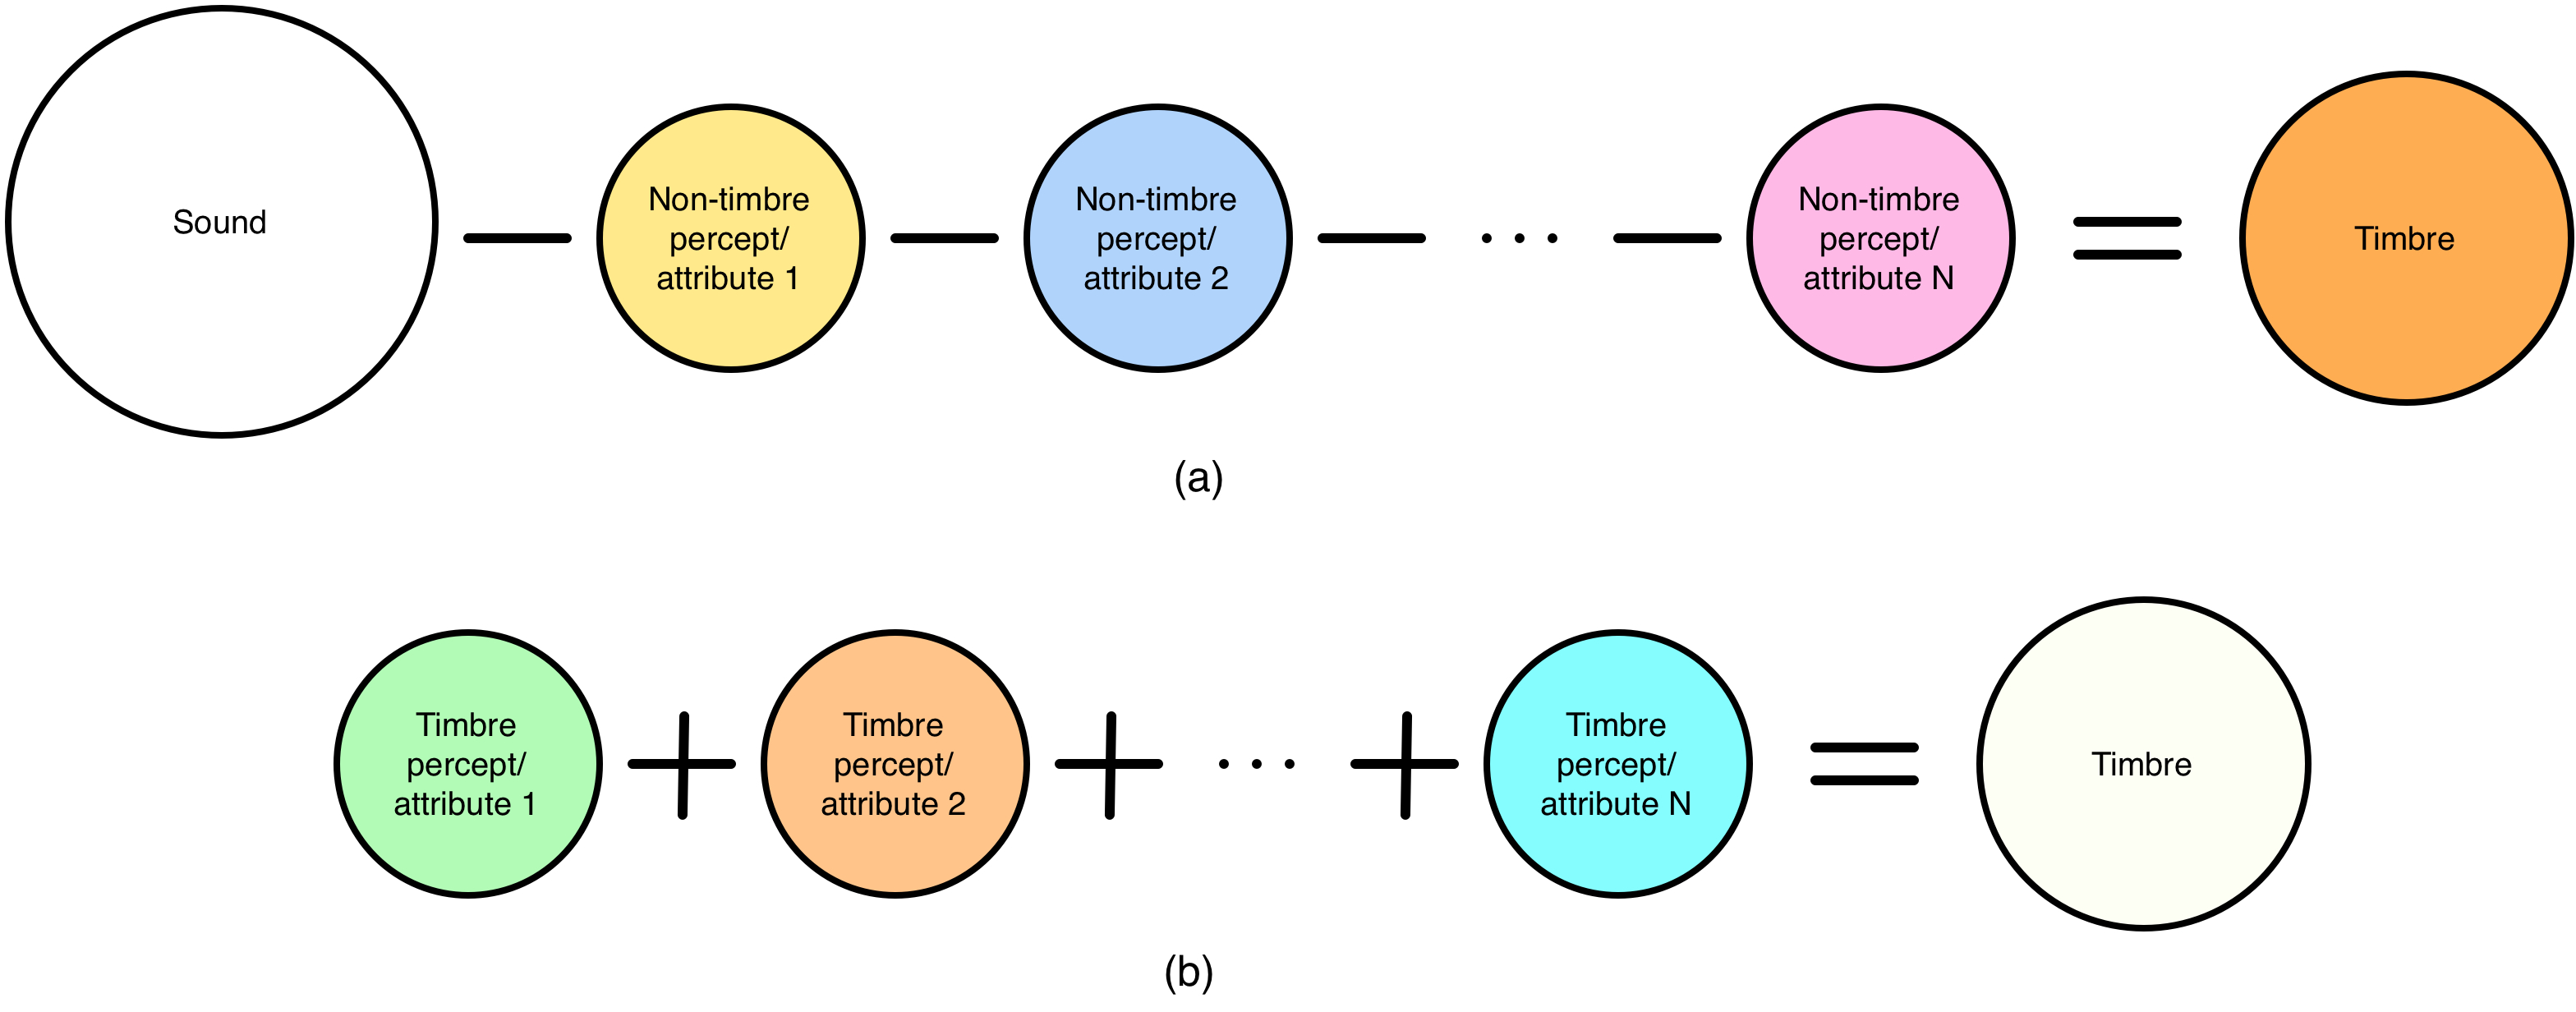
\includegraphics[scale=0.45]{SubtractiveVsAdditive}
\caption[Subtractive vs. additive timbre definitions]{Visual representations of (a) subtractive and (b) additive definitions of timbre.}
\end{center}
\vspace{6pt}
\end{figure}
Additive definitions explain timbre by associating it with things that it \textit{is}, while subtractive definitions attempt to explain timbre by defining what it \textit{is not}. The subtractive definition, most common in the literature, explains timbre as being the characteristics of a sound left over after removing pitch and loudness \cite[p. 45]{Wessel:1979tg} \cite[p. 225]{Toiviainen:1998hs}. Ciglar points out that this definition assumes that every sound (with the property of timbre) has a definitive pitch in the first place and suggests that this implies that unpitched sounds do not have timbre \cite[p. 7]{Ciglar:2009uf}. A possible addendum to this definition may be that timbre is what is left after removing loudness and pitch, assuming a pitch even exists to be removed. However, such a definition is still unsatisfactory, and this is why a good deal of research has been carried out to define timbre using an additive definition.

In order to build an additive definition of timbre, one typically performs controlled perceptual similarity tests, uses the results to build a subjective timbre space where distances are semantically meaningful, and then associates the axes of this space with acoustic features \cite[p. 1]{Pampalk:2008xz}. Some of the earliest studies of subjective timbre spaces were performed separately by Grey and Wessel \cite{Grey:NoRead, Wessel:1979tg}. Both use multidimensional scaling algorithms (MDS) to develop a timbre space from pairwise subjective similarity tests. MDS allows one to generate a space, typically two- or three-dimensional (though by no means limited to these), given a set of distance measurements between points, where the cumulative error in the distances provided between the points is minimized. In other words, MDS provides a way to generate a Euclidean space given a set of subjective measurements. However, in order to assign acoustic features to the axes resulting from MDS analysis on subjective measurements, one is left to find correlations between these axes with tested features. For example, using a two-dimensional timbre space, Wessel finds that the axes correlate with the spectral envelope and the nature of the onset transient \cite[p. 48]{Wessel:1979tg}. However, definitively assigning features to these axes based simply on correlation is misguided. As Caclin, McAdams, Smith, and Winsberg point out in their investigation into the properties of timbre, ``Given the multiplicity of acoustical parameters that could be proposed to explain perceptual dimensions, one can never be sure that the selected parameters do not merely covary with the true underlying parameters'' \cite[p. 2]{Caclin:2005il}. 

Another problem with this approach is that MDS forces the user to choose the dimensionality of timbre space a priori, which will result in a feature set to explain timbre that may either contain too much or too little information.

Generating a perceptual timbre space using MDS also can be handicapped if not given a wide variety of timbral material that sufficiently covers the perceptual space. As Seago, Holland, and Mulholland note, if not using a wide enough variety of timbral material ``a sound in MDS space may have perceptually important features that no other sounds in the same space have---and, by the same token, two sounds could occupy the same location in a given MDS perceptual space, and nevertheless be audibly different'' \cite[p. 3]{Seago:2008ya}.

Yet another drawback of subjective testing is discussed by Prandoni \cite{Prandoni:1994th}. He notes that many of the pairwise similarity tests for timbre space construction are performed using common instrument sounds. Prandoni writes that this is a major problem in that ``the subjective ratings thus obtained are often affected by the listener's high-level notions of the structural features of the playing instruments rather than being a pure combination of sounds'' \cite[p. 2]{Prandoni:1994th}. Nicol's previously referenced statements on ecological listening seem to bolster this hypothesis. 

Prandoni further points out that these studies find that features related to the attack and steady-state spectral envelope are often found to be highly correlated with the resultant timbre space axes because these are the features that ``remain constant among different nuances of color in recognizing an instrument'' \cite[p. 8]{Prandoni:1994th}. Therefore, it is not clear whether other features beyond those that allow discrimination between instruments and instrument classes are perceptually relevant, but just not useful in the discrimination task. 

From Prandoni's comments, one wonders if the features derived from these tests may best describe the intuition of timbre that is tied to the sound-producing body that created it, rather than that which relies solely on the sonic characteristics of the sound. This is supported by the fact that these tests ask a subject to note the similarity between whole instrument tones, rather than between attacks or steady-state portions separately. The result is that a single note played by an instrument will be placed as a single point in timbre space, rather than trace out a trajectory. In other words, each point in timbre space will correspond to a sound that has an attack, sustain, and release. The fact that each point is guaranteed to have an attack is especially important because 'shape of the attack' is one of the most often cited timbral features.

Thus, there is a large body of literature one may look to when deriving timbre features for the type of timbre that focuses on the sound-producing body rather than a single sonic character. In the latter case, one would not expect each sonic character to contain an attack, for example, and so the features that arise from subjective testing (via strong correlations with the resultant MDS axes) may not be relevant. Instead of each sound in a subjective test being represented by a single point in timbre space, a more compatible representation with the concept of sonic character would be that each instrument sound generates a trajectory of points throughout timbre space as its character evolves. 

In Nicol's treatment of what he terms subjective and objective timbre spaces, he writes that the single point vs trajectory delineation is one of the main differentiating characteristics between them \cite[p. 56]{Nicol:2005rp}. In an objective timbre space, each moment in time is represented by a point. As time evolves, a trajectory is traced out through timbre space. This representation falls more in line with Johnson and Gounaropoulos' local timbre distinction \cite{Johnson:2006pi} and agrees with our intuition of what points should represent when viewing timbre as a single sonic character. It follows from this representation that timbre similarity calculations in this space (between two sounds whose sonic characteristics evolve over time) will necessarily incorporate information regarding temporal evolution. Such a similarity calculation is required when trying to find optimal matches to time-varying timbral content.

It is clear from the discussion above that the concept of timbre is complex and that there are inherent problems in describing it in both subtractive and additive terms. As noted, these issues propagate into the domain of timbre feature design, which we investigate further in developing our approach to quantify timbral similarity (see Chapter III - Approach).
\vspace{12pt}
\section{Sound Synthesis}

Timbre is a fundamental parameter of music, yet total and precise timbral control cannot be realized---or, at the very least, is severely limited---by acoustic means. Even the most skilled players are constrained by the physics of their instruments' sound production mechanisms \cite[p. 11]{Wessel:2002uk}. However, with the advent of digital technology, the sound generator can be separated from its control interface and, as a consequence, no longer needs to be reliant on its physical properties \cite[p. 1]{Malloch:2006jb}. The resulting timbral freedom introduced by digital technology augmented the already increasingly important role timbre had taken in Western compositional practice starting from the turn of the twentieth century \cite[p. 1]{Klingbeil:2009lo}. In investigating the increasingly common compositional use of timbre, Nicola Bernardini and Jran Rudi write that by providing a ``different, deeper and total control over timbre [computer music composition has placed a] stronger focus on the timbral aspects of composition -- on the micro-level.'' \cite[p. 3]{Bernardini:2001kc}. This increased focus on timbre has spawned the design of numerous sound synthesis algorithms over the past fifty years in hopes to provide the composer with the level of control over timbre that they have enjoyed for years with pitch and loudness.

The different approaches used in designing synthesis algorithms have varied widely throughout the history of sound synthesis. A number of sources provide surveys of the most popular techniques \cite{Roads:NotRead, Miranda:NotRead, Cook:NotRead}. Miller Puckette's \textit{The Theory and Technique of Electronic Music} stands out among the rest in that he not only describes the underlying mathematics behind a number of different synthesis algorithms, but he also supplies the user with a blueprint for design and timbral exploration \cite{Puckette:2007ai}. This book, in combination with Puckette's earlier paper \textit{Combining Event and Signal Processing in the MAX Graphical Programming Environment} \cite{Puckette:NoRead2}, provides a comprehensive look into designing synthesis algorithms using a graphical programming environment. 

The intent of these writings is not to compare and contrast the efficacy of the algorithms presented, but instead only to illustrate their inner workings. However, when a composer is ready to select a specific synthesis algorithm to work with, the results of such comparisons are paramount to the decision-making process. In order to assess the strengths and weaknesses of each algorithm, one must have a clear understanding of the desirable properties of a timbre producer/manipulator.

These properties have been discussed by a number of respected figures in the field of computer music at various levels of depth \cite{III:1991hc, Wessel:2002uk, Jaffe:1995fv}. Smith's treatment is relatively superficial in large part because these properties are not his paper's main focus. Jaffe's list of properties presume that a synth's main purpose is to mimic a real-world sound-producing body, which is not always necessarily the case. Wessel and Wright mix the desirable properties of synthesis algorithms with those of control interfaces, often blurring the lines between the two within the same listed property. Most recently, in his treatment of composing with timbre, Nicol \cite[p. 40]{Nicol:2005rp} provides four desirable properties for an ideal synthesizer: ``fast synthesis'' (i.e. computational efficiency); a ``wide timbral range'' (i.e. the ability to produce any desirable timbre); ``easy parameterization'' (i.e. an intuitive, low-dimensional mapping between parameters and sound); and ``low data requirements'' (i.e. low memory storage requirements). In other words, Nicol believes that an ideal synthesizer will provide the composer with an intuitive, low-dimensional parameter set that they may use to achieve (and manipulate) any desired timbre. Additionally, the underlying synthesis algorithm will ideally work in real-time and use a small amount of memory.

One of the most comprehensive comparative studies of synthesis algorithms is presented by Tolonen, V\aa lim\aa ki, and Karjalainen \cite{Tolonen:1998bh}. In this report, the authors categorize each synthesis algorithm under evaluation into one of four groups: abstract algorithms; sampling and processed recordings; spectral methods; and physical models (as originally proposed by Smith \cite{III:1991hc}). Among the many algorithms treated, Tolonen et al. choose the most popular (also known as \textit{classical} synthesis algorithms) to evaluate, and find that variants within each category perform similarly to their classical counterpart in regards to the proposed criteria \cite[p. 101]{Tolonen:1998bh}. The classical synthesis methods investigated in their study were sampling synthesis (sampling and processed recordings), additive synthesis (spectral methods), FM synthesis (abstract algorithms), and digital waveguide synthesis (physical models). A more complete list of algorithms can be found in Table 1.
\begin{table}[h!]
\vspace{24pt}
\begin{center}
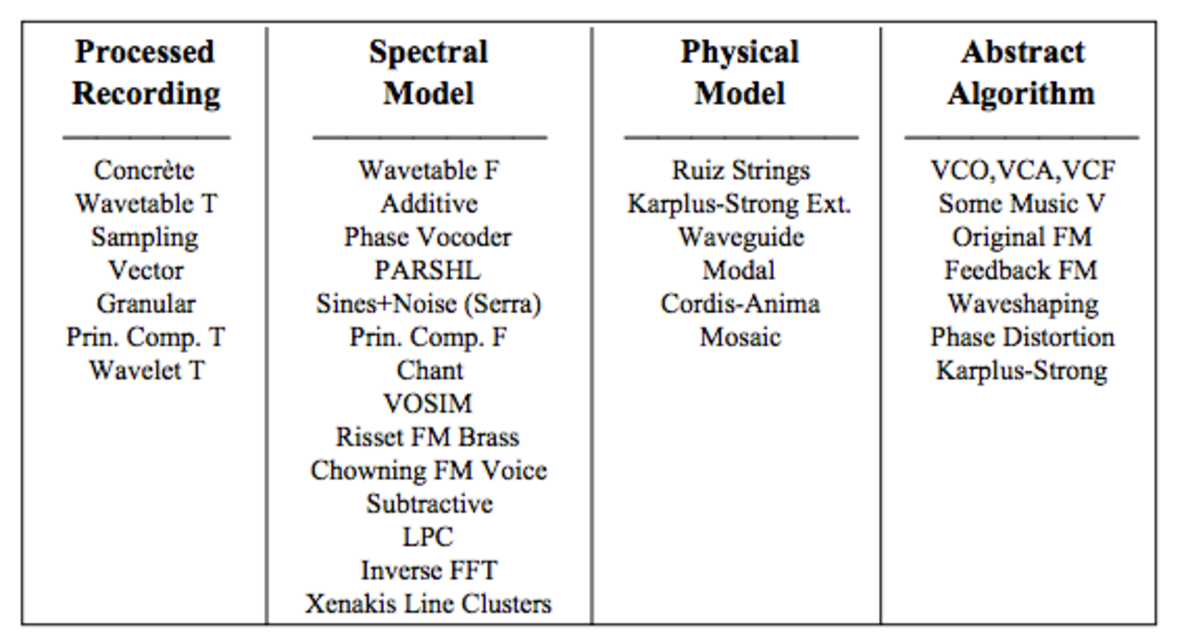
\includegraphics[scale=0.7]{SynthesisTechniqueTaxonomy}
\caption[Synthesis technique taxonomy]{A synthesis technique taxonomy proposed by Smith \protect\cite{III:1991hc}.}
\end{center}
\vspace{6pt}
\end{table}

Sampling synthesis (see Figure 2) ``is a method in which recordings of relatively short sounds are played back'' \cite[p. 10]{Tolonen:1998bh}. 
\begin{figure}[h!]
\begin{center}
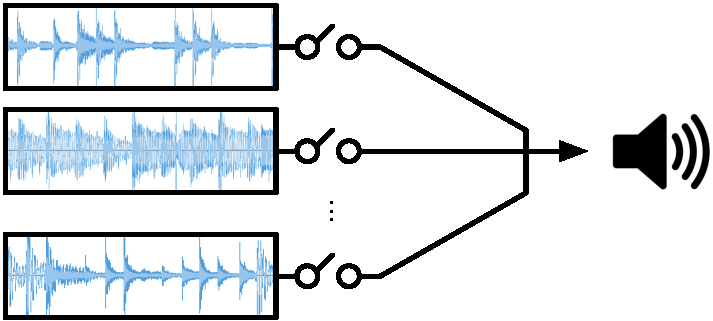
\includegraphics[scale=0.8]{SamplingSynthesis}
\caption[Sampling synthesis]{Sampling Synthesis}
\end{center}
\vspace{6pt}
\end{figure}
Using sampling, one can turn any audio recording into a musical instrument by simply assigning the playback of the recording to a switch \cite[p. 1]{Heise:2009sp}. This type of synthesis dates back to the 1920's and certainly became prominent in 1950 when Pierre Schaeffer founded the Studio de Musique Concrete in Paris \cite[p. 3]{Tolonen:1998bh}. Like all sampling and processed recordings methods, sampling synthesis' flexibility is dependent on the size of the database containing the pre-recorded audio segments. Thus, to obtain a truly flexible sampling synthesizer ``the required amount of memory storage is huge'' \cite[p. 11]{Tolonen:1998bh}. As the flexibility of the system grows and one has enough material to generate small variations in timbre, doing so becomes more difficult as the number of samples to choose from during any single discrete movement in timbre space becomes unwieldy. Thus, while sampling synthesis is computationally efficient and requires a low-dimensional parameter set, there is a fundamental tradeoff between its ability to generate a wide variety of timbral material and the amount of memory it requires. It is also nontrivial to transform a given timbre in a smooth way, which, in his more recent survey of synthesis techniques, Smith writes is the true ``fundamental problem with sampling synthesis'' (2006, p. 22).

Granular synthesis (see Figure 3) ``is a set of techniques that share a common paradigm of representing sound signals by \textit{sound atoms} or grains...the synthetic sound signal is composed by adding these elementary units in the time domain'' \cite[p.13]{Tolonen:1998bh}. 
\begin{figure}[h!]
\begin{center}
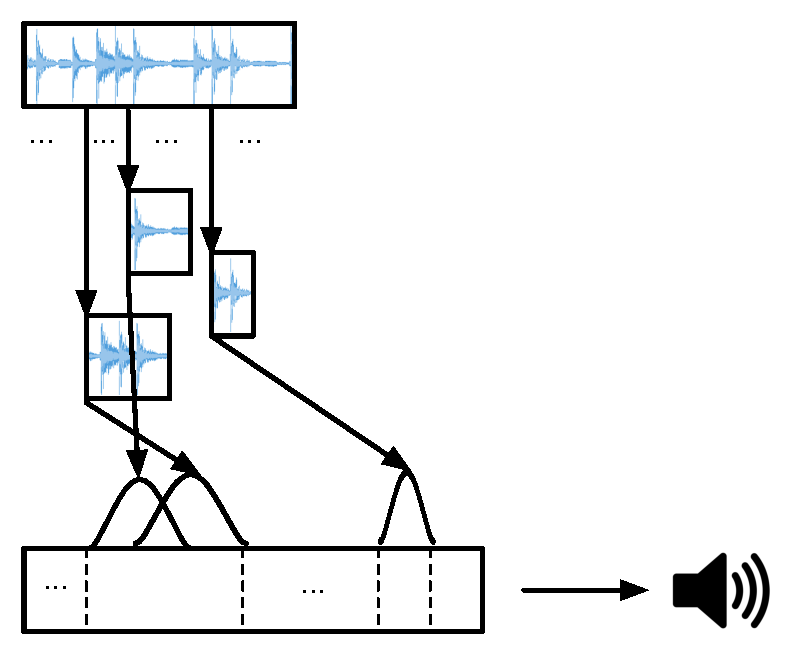
\includegraphics[scale=0.8]{GranularSynthesis}
\caption[Granular synthesis]{Granular Synthesis}
\end{center}
\vspace{6pt}
\end{figure}
In his dissertation on analysis/synthesis techniques (which will be covered later), Klingbeil adds that ``granular synthesis may be viewed as a particular specialization of sampling synthesis...[It] offers the possibility to decouple the time and frequency evolution of a sound, as well as impart particular characteristics modulating between rough, smooth, or stochastic textures'' \cite[p. 6]{Klingbeil:2009lo}. Thus, unlike sampling synthesis, granular synthesis allows one to transform smoothly between timbres. However, this comes at the price of a higher dimensional parameter space, forcing the user to specify ``the shape of the overall \textit{cloud}, the fundamental frequency, the way in which the individual grains are generated, the structure of the individual grains used, etc'' \cite[p. 5]{Johnson:1998sh}. In Nicol's dissertation investigating mappings between synthesis parameter spaces and timbre spaces, he notes that the non-intuitive mapping between this high dimensional parameter space and timbre space makes ``emulation of target timbres a non-trivial process'' \cite[p. 49]{Nicol:2005rp}. Granular synthesis requires less memory than sampling synthesis, but is also less efficient (although real-time algorithms do exist). Vercoe, Gardner, and Scheirer point out that granular synthesis is ``best suited to the generation of noisy or textural sounds like water, wind, applause, and fire'' \cite[p. 6]{Vercoe:1998hh}.

Additive synthesis (see Figure 4) ``is a method in which a composite waveform is formed by summing sinusoidal components to produce a sound'' \cite[p. 17]{Tolonen:1998bh}. 
\begin{figure}[h!]
\vspace{24pt}
\begin{center}
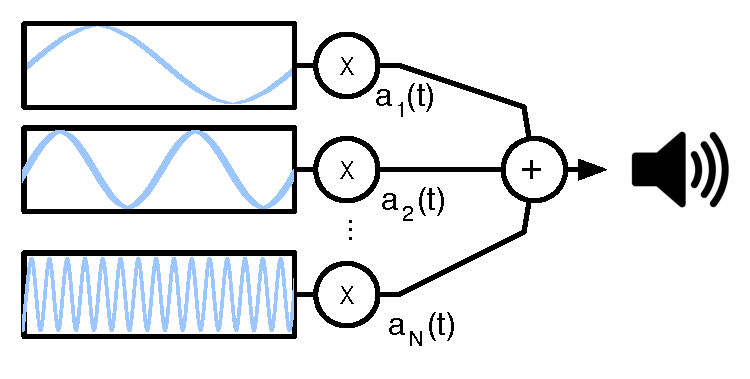
\includegraphics[scale=0.8]{AdditiveSynthesis}
\caption[Additive synthesis]{Additive Synthesis}
\end{center}
\vspace{6pt}
\end{figure}
Based on Fourier analysis, ``additive synthesis can in theory synthesize arbitrary sounds if an unlimited number of oscillators is available'' \cite[p. 94]{Tolonen:1998bh}. However, as the numbers of oscillators increase, so does the number of controllable parameters. Consequently, there is a fundamental tradeoff between flexibility and controllability with respect to the number of oscillators used \cite[p. 7]{Klingbeil:2009lo}. It is because of this that additive synthesis is best utilized for generating harmonic or quasi-harmonic signals where little noise is present \cite[p. 5]{Vercoe:1998hh}. Additive synthesis also requires a number of parameters to be changed simultaneously in order to move a small distance in timbre space, which is unattractive. The desirable properties that additive synthesis satisfies are low storage (although the control data can require a lot of memory) and the ability to generate, in theory, any timbre, but its parameter space is high-dimensional and difficult to control as a result.

Subtractive synthesis (see Figure 5) is similarly based on Fourier analysis, but works by subtracting sinusoids from a spectrally rich source to generate material rather than building up material by adding sinusoids together, as in additive synthesis. 
\begin{figure}[h!]
\vspace{12pt}
\begin{center}
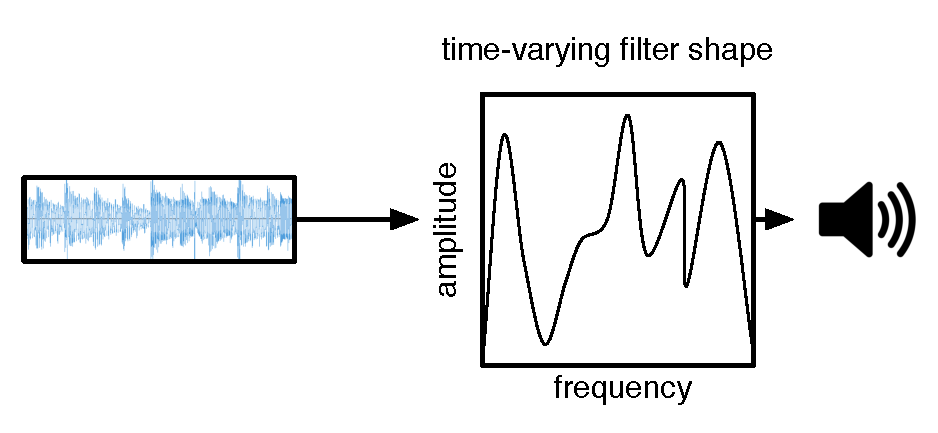
\includegraphics[scale=0.8]{SubtractiveSynthesis}
\caption[Subtractive synthesis]{Subtractive Synthesis}
\end{center}
\vspace{6pt}
\end{figure}
The \textit{subtraction} is performed by a time-varying filter whose coefficients are supplied by the user. In order to achieve complex and temporally evolving sounds, the parameter space can grow to the size of additive synthesis and therefore will suffer from the same controllability issues \cite[p. 48]{Tolonen:1998bh}. If one uses a simple network of filters to try to reduce the size of the parameter space, ``the resulting tones have a distinctive \textit{analog synthesizer} character that, while sometimes desirable, is difficult to avoid'' \cite[p. 5]{Vercoe:1998hh}. Thus, one must trade timbral flexibility with the controllability of the algorithm. Similar to additive synthesis, the control data can require a lot of memory during sound production. Also, the efficiency of the algorithm and the facility to move around timbre space varies with the complexity of the time-varying filter or network of filters.

FM synthesis (see Figure 6), in its most basic form, contains two oscillators, which are connected so that one oscillator's waveform modulates the frequency of the other. 
\begin{figure}[h!]
\vspace{24pt}
\begin{center}
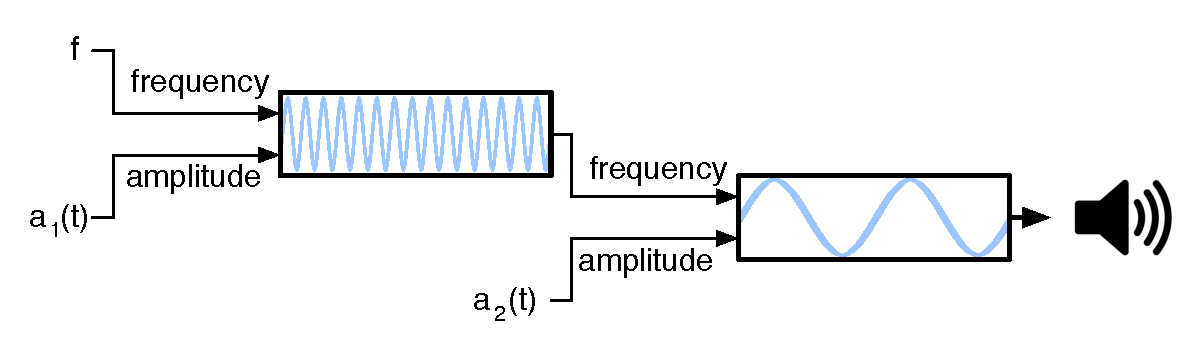
\includegraphics[scale=0.65]{FMSynthesis}
\caption[FM synthesis]{FM Synthesis}
\end{center}
\vspace{6pt}
\end{figure}
There are only a few parameters with which to generate a large range of timbral material, which is desirable, but due to an inherent nonlinear mapping between parameter space and control space, ``FM has become widely regarded as a difficult synthesis type to control'' \cite{Mitchell:2007fe}. This is for two reasons. First, the nonlinearity provides a non-intuitive relationship between a given set of parameters and the sound it produces \cite[p. 45]{Nicol:2005rp}. Second, a  nonlinear mapping means that small changes in the input parameters can map to large changes in the timbre and thus fine timbral manipulation can be difficult \cite[p. 2]{Jaffe:1995fv}. Another undesirable quality of FM synthesis is that the characteristic FM sound is ``fairly metallic, so the FM output is often filtered in order to produce a more natural sound'' \cite[p. 45]{Nicol:2005rp}. The benefits of FM synthesis are that is ``is very cheap to implement, uses little memory, and [as previously mentioned] the control stream is sparse'' \cite[p. 92]{Tolonen:1998bh}.

Digital waveguides (see Figure 7) are ``based on a general solution of the wave equation in a one-dimensional homogeneous medium'' \cite[p. 63]{Tolonen:1998bh}. 
\begin{figure}[h!]
\begin{center}
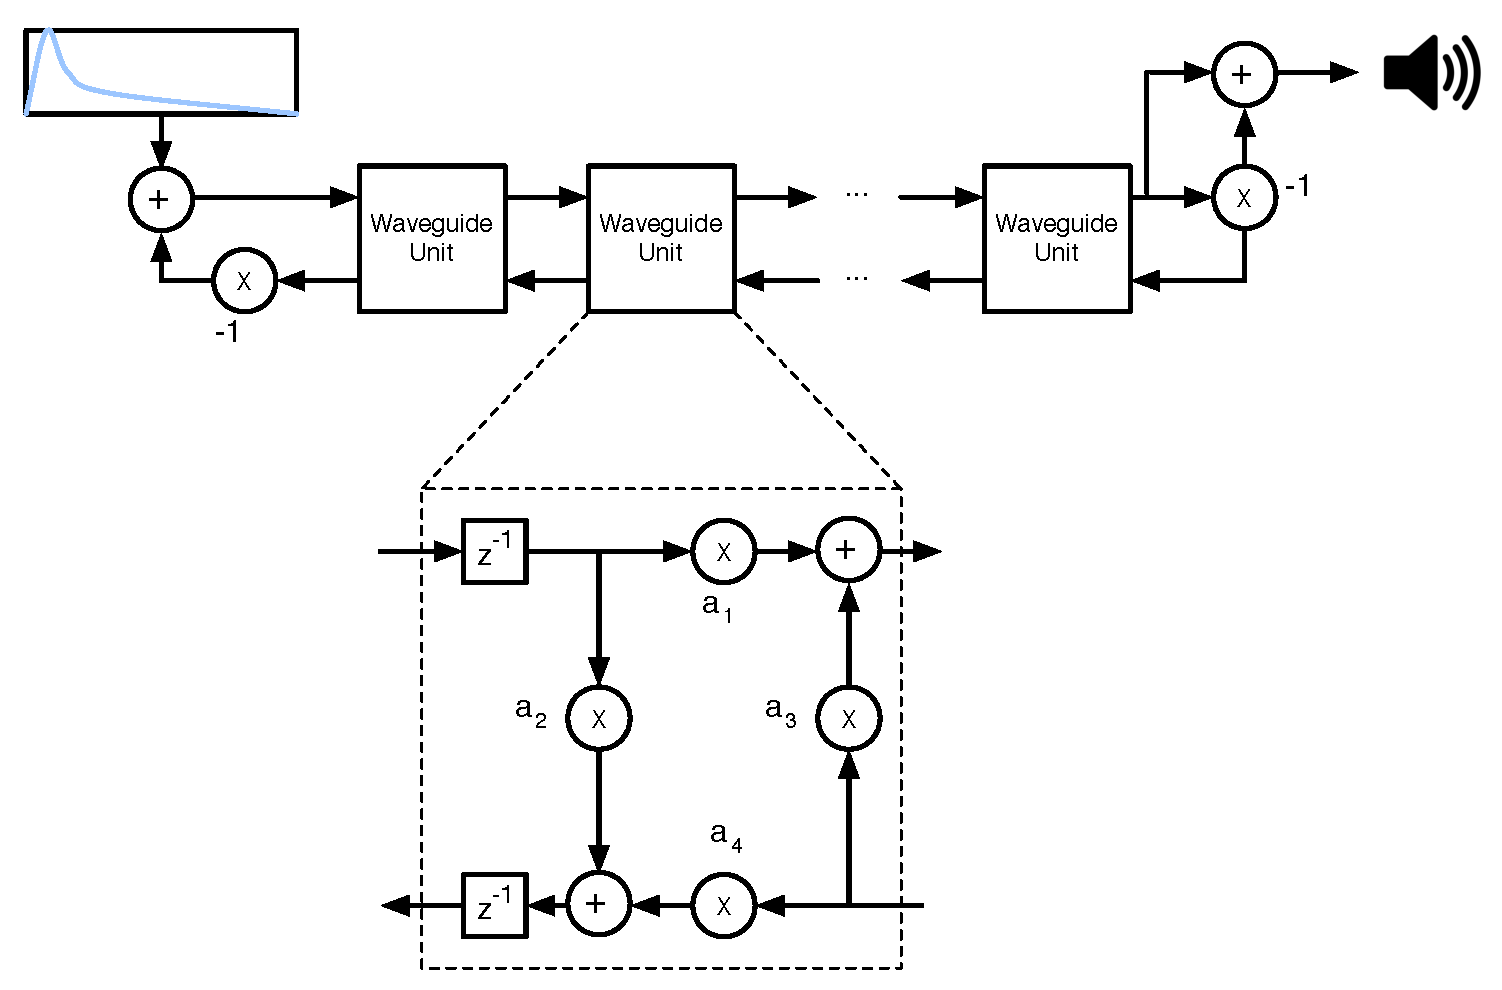
\includegraphics[scale=0.55]{DigitalWaveguideSynthesis}
\caption[Digital waveguide synthesis]{Digital Waveguide Synthesis}
\end{center}
\vspace{6pt}
\end{figure}
They are basic linear time-invariant (LTI) structures that allow one to develop physical models of various instruments. Their parameters are intuitive and small in number, aiding in timbral manipulation. However, specific waveguide networks are designed to imitate a single sound-producing body and therefore are timbrally restricted in comparison to additive synthesis. Also, as Smith comments in his seminal paper on digital waveguides, ``new models must be developed for each new kind of instrument, and for many instruments, no sufficiently concise algorithm is known'' \cite[p. 86]{III:1992zn}. In fact, as Tolonen et al. point out, any sound producing object that requires a two- or three-dimensional waveguide mesh to represent its governing physics will be computationally expensive to model and, consequently, only simple physical models based on waveguides will be able to run in real-time \cite[p. 99-100]{Tolonen:1998bh}. Thus, digital waveguides provide a low-dimensional, intuitive parameter set and low storage requirements, but can be computationally expensive for complex sounds and require separate topologies for each region of timbre space \cite[p. 50]{Nicol:2005rp}.

The above discussion illustrates a fundamental tradeoff between versatility and control that all individual synthesis topologies face. The in-depth comparative study of various sound synthesis techniques, carried out by Tolonen et al., elucidates the strengths and weaknesses of each algorithm in regards to this tradeoff as well as practical issues related to implementation. However, one practical issue of utmost importance that is not covered in this study is whether each algorithm provides a mechanism by which to realize a specific target timbre. If such a mechanism does not exist, the resultant algorithm would be, at best, as useful as an instrument capable of producing any pitch and offering fine pitch control, but lacking deterministic means to produce a specific desired pitch. Chafe, in presenting a historical perspective on the many ways synthesis has influenced and benefitted composition over the last fifty years, writes that, historically, imitation has been one of the main uses of sound synthesis since its inception \cite[p. 2]{Chafe:1999bx}. Thus, the importance of being able to achieve a specific desired timbre cannot be overstated.

For sample synthesis, one only needs to record the desired sound and store it for later retrieval. However, as previously stated, as the number of desired timbres increases the storage requirements become difficult to manage. Thus, more sophisticated methods are required. For the other synthesis algorithms discussed, there are unfortunately no obvious ways to extract the precise parameter set for a desired timbre. A body of research has emerged specifically to develop methods for this task. These methods are generally referred to as \textit{parameter estimation} or \textit{re-synthesis} techniques.
\vspace{12pt}
\section{Parameter Estimation}
Estimating synthesis parameters for a target timbre is a difficult problem (see Figure 8). 
\begin{figure}[h!]
\begin{center}
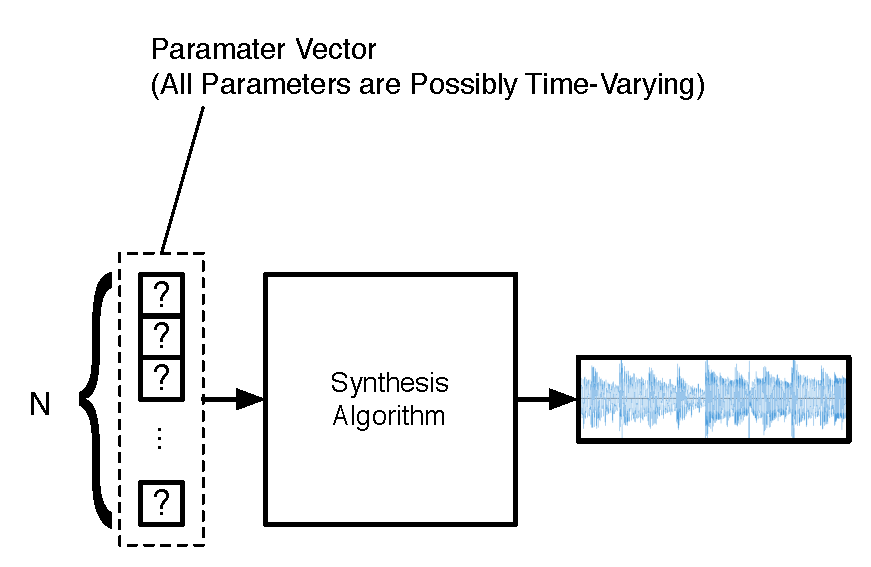
\includegraphics[scale=0.7]{ResynthesisProblem}
\caption[Producing a target timbre]{The Task of Producing a Target Timbre}
\end{center}
\vspace{6pt}
\end{figure}
Johnson and Gounaroloulos \cite{Johnson:2006pi} write that that it is not possible to find an appropriate mapping from the input parameters to a desired result unless ``[users] have a very strong understanding of the underlying mechanisms that produce the sound, or a large amount of `trial-and-error' experience with generating timbral changes within a system'' \cite[p. 1]{Johnson:2006pi}. However, even with both a strong understanding of a sound synthesis algorithm's sound producing mechanisms and extensive experience using the algorithm to explore timbre, the ability to realize a particular point or region in timbre space can be time-consuming at best, and is often infeasible, as discussed in Heise et al.'s paper on parameter estimation \cite[p. 1]{Heise:2009sp}. The requirement that a composer be versed in signal processing theory and, quite often, computer programming in order to even begin to search efficiently in timbre space is not ideal. Mitchell notes that such a requirement often leaves the composer ``more concerned with the scientific process [driving the algorithm] than artistic creativity'' \cite[p. 1]{Mitchell:2007fe}.

As opposed to leaving the task of target timbre discovery to the composer, re-synthesis and parameter estimation techniques attempt to automatically fit the parameters of a sound synthesis algorithm to imitate a target sound (see Figure 9). \begin{figure}[h!]
\begin{center}
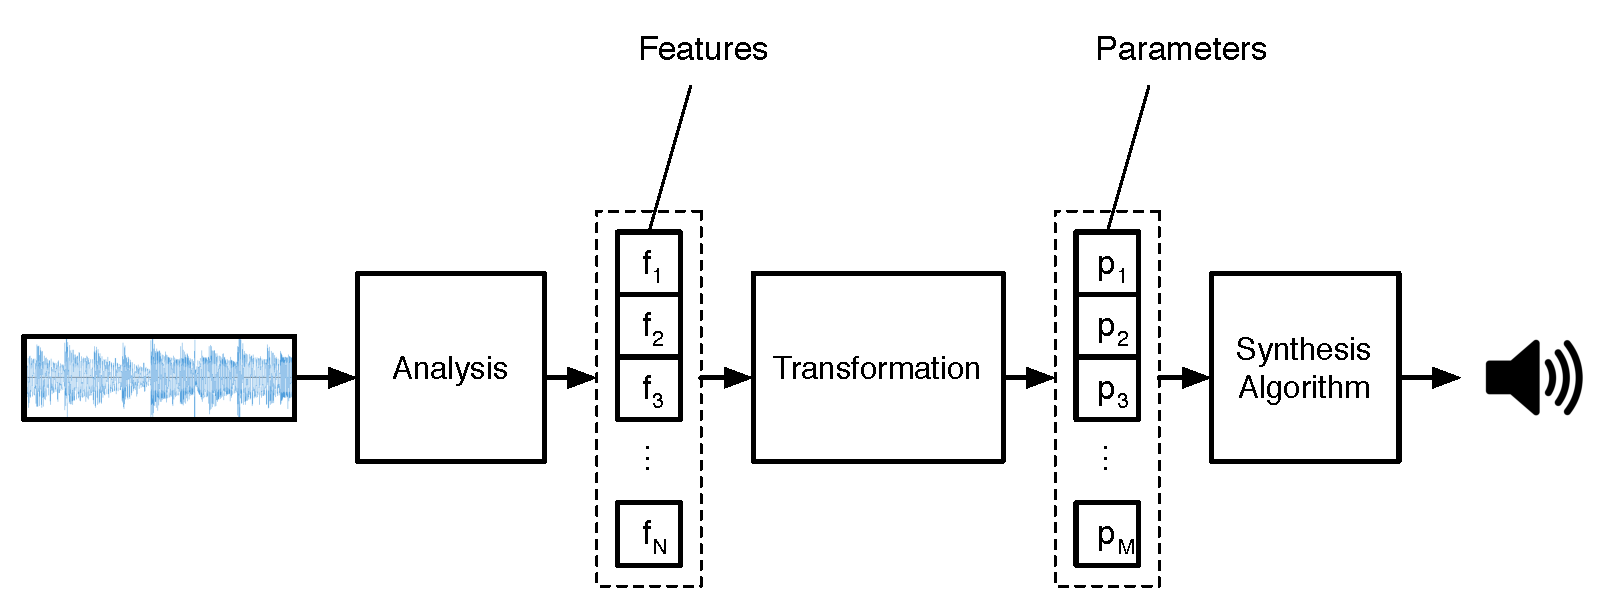
\includegraphics[scale=0.5]{ResynthesisIdea}
\caption[Re-synthesis]{Re-synthesis Approach}
\end{center}
\vspace{6pt}
\end{figure}
Specifically, re-synthesis uses the results of a target signal's analysis to fit parameters to an underlying synthesis algorithm. Once an acceptable parameter set has been found, the user is left to explore the space around the target using the underlying synthesizer. This means that a re-synthesis technique built upon a specific synthesis algorithm will leave the user with an instrument, `tuned' to the desired timbre, that suffers from the same pitfalls associated with the algorithm. It is therefore useful to categorize re-synthesis techniques based on their underlying synthesis algorithms, so that one may compare these techniques within the proper context.

An in-depth comparison of some of the most ubiquitous re-synthesis techniques can be found in Klingbeil's dissertation \cite{Klingbeil:2009lo}. However, one must look beyond this source in order to evaluate promising state-of-the-art techniques from each synthesis category proposed by Smith \cite{III:1991hc}.

One of the most popular re-synthesis techniques utilizing a sampling synthesis method is concatenative synthesis (see Figure 10). 
\begin{figure}[h!]
\begin{center}
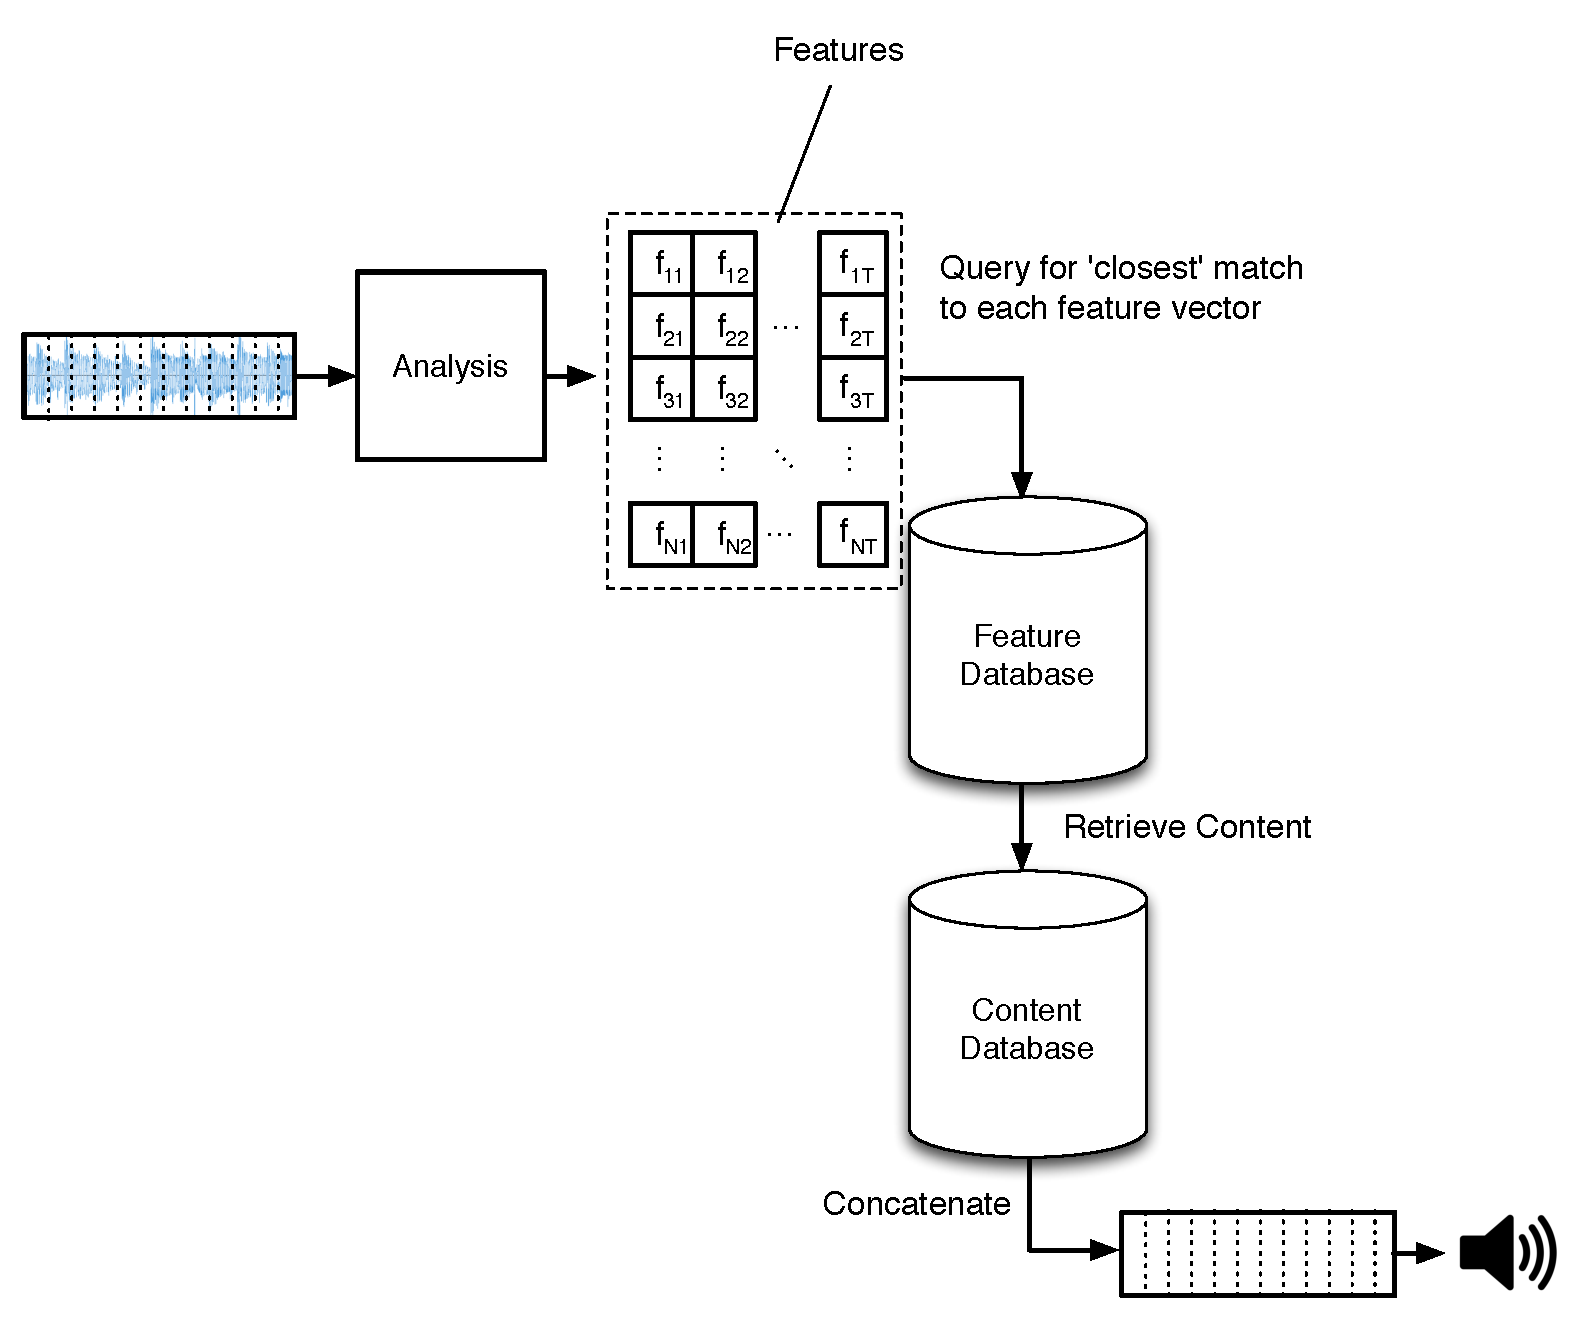
\includegraphics[scale=0.55]{ConcatSynth}
\caption[Concatenative synthesis]{Concatenative Synthesis}
\end{center}
\vspace{6pt}
\end{figure}
Concatenative synthesis, as described by Diemo Schwarz, ``use[s] a large database of source sounds, segmented into units that match best the sound or musical phrase to be synthesized, called the target'' \cite[p. 1]{Schwarz:2006gr}. In principle, concatenative synthesis can be used to match any type of feature (e.g. timbre, pitch, loudness). To differentiate timbral matching from other objectives, the term \textit{musical mosaicing} is used, a process first developed by Zils and Pachet \cite{Zils:2001bd}. 

In order to determine the best timbral match in the database to a given target one must rely on a perceptual distance measure. Deriving such a measure is complicated (as will be discussed later) \cite[p. 13]{Schwarz:2006gr}. In addition to searching for the best matching units, musical mosaicing also typically constrains the sequencing of these units to ensure a smooth timbral development \cite[p. 1]{Zils:2001bd}. In order to achieve accurate re-synthesis, a large database of units is required to meet both local and global constraints while providing a high-fidelity solution. As the size of this database increases an efficient search becomes difficult. The length of this search may not be problematic for a composer interested in matching one particular target, but if timbral exploration around the target is desired, the search for a new sequence for every slight timbral variation becomes a prohibitive bottleneck \cite[p. 11]{Schwarz:2006gr}.  If discontinuities between units and imprecise unit matching is acceptable however, such a search can usually be run in realtime.

For example, Bonada and Serra have developed a system where they pre-compute timbral features over an extremely large database of vocal sound units that sufficiently cover their vocal feature space, and allow a user to map performance trajectories to that space, retrieving the closest units to that trajectory, and concatenating them to produce an output signal \cite{Bonada:2007bs}. They call this \textit{performance sampling} \cite[p. 67]{Bonada:2007bs}.Their system is able to generate a wide variety of vocal timbral evolutions. However, as noted by the authors, the storage requirements are large in order to model only a small region of timbre space and they have yet to determine a way to limit undesirable discontinuities between ``breathy to non-breath connections'' \cite[p. 78]{Bonada:2007bs}.

An interesting granular synthesis re-synthesis techniques was proposed by Johnson \cite{Johnson:1998sh}. He provides a system to the user that allows them to score a number of randomly generated output sounds based on their similarity to a user-defined target. These scores are used to ``push'' the parameter set corresponding to each generated output towards the target sound, and the user scores the results again. This process continues until the target is reached  \cite[p. 2]{Johnson:1998sh}. The system works well as long as the user commits to the process, but because it is not completely automated, it is not an ideal solution.

There are several popular re-synthesis methods that employ spectral models, which fit the parameters of additive synthesizers. Of these, the most popular are the phase vocoder and spectral modeling synthesis (SMS).

The phase vocoder (see Figure 11) was developed at Bell laboratories in 1966 and first introduced to the music community as a re-synthesis tool a decade later by Moorer \cite{Moorer:1978ge}. \begin{figure}[h!]
\vspace{24pt}
\begin{center}
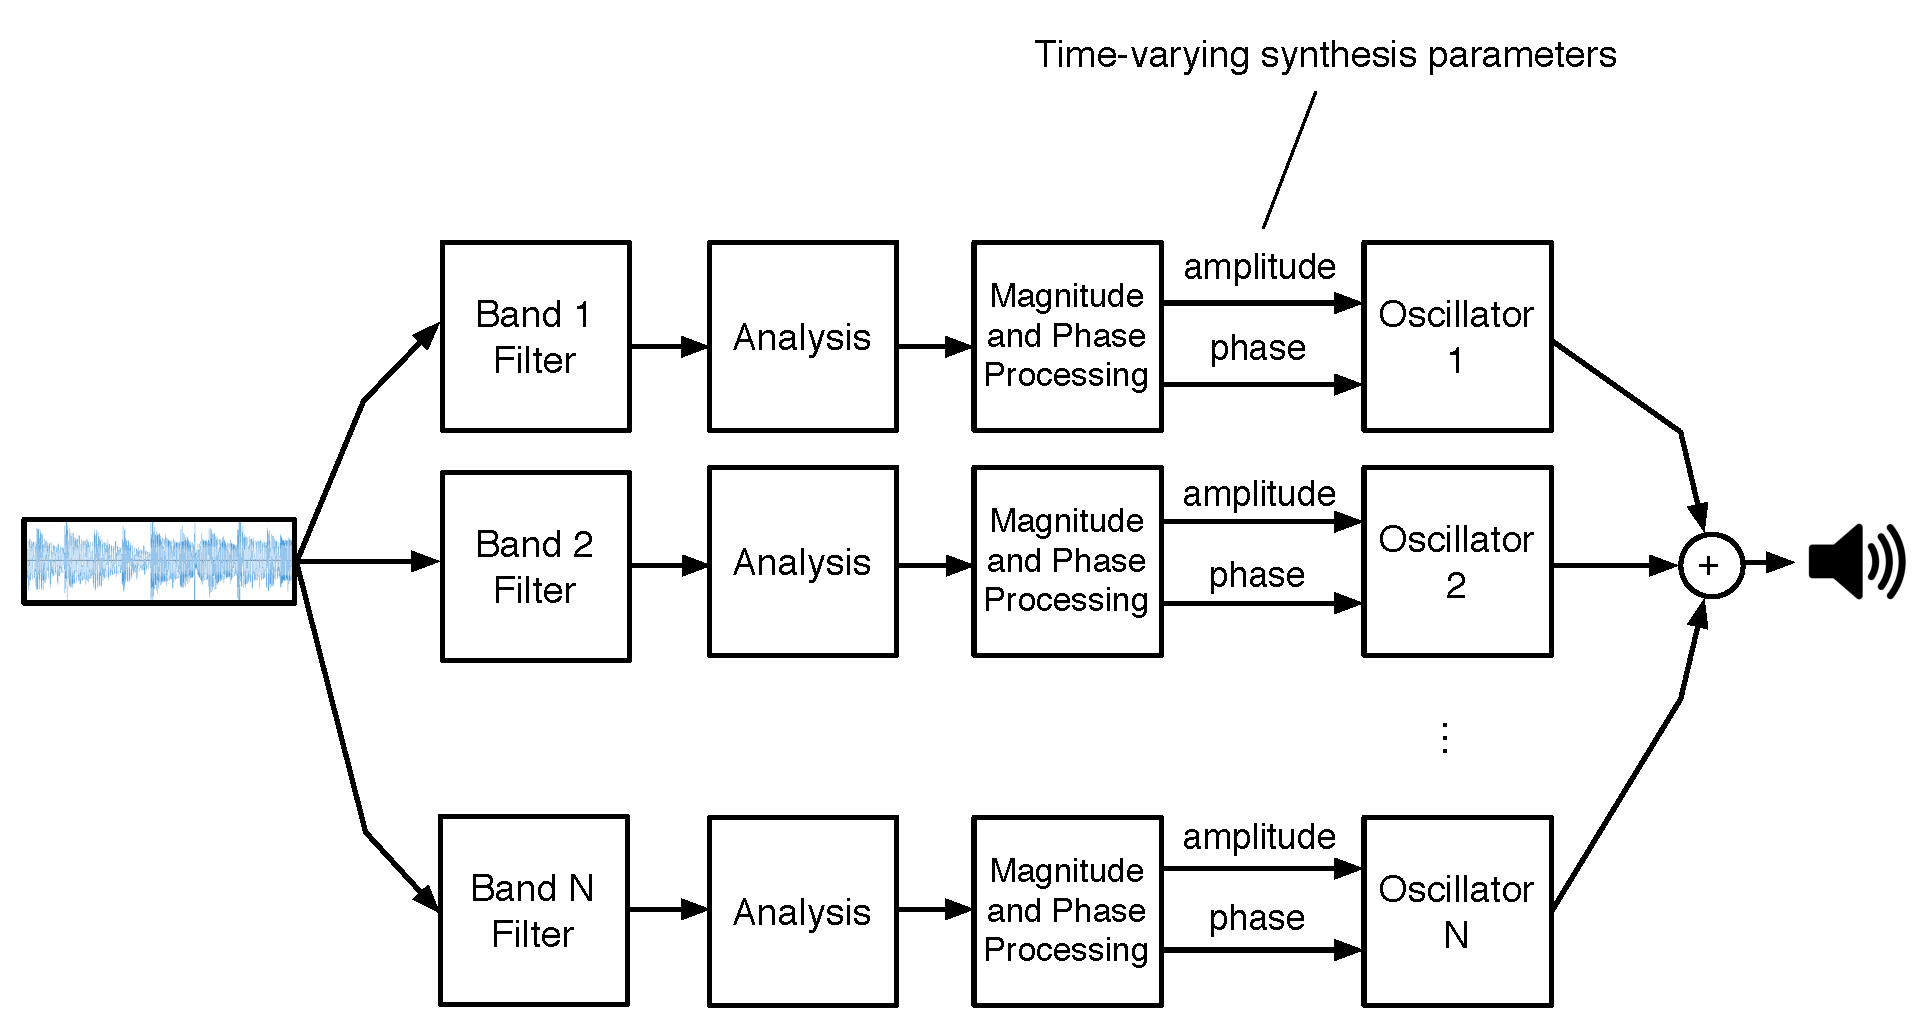
\includegraphics[scale=0.45]{PhaseVocoder}
\caption[Phase vocoder]{Filter-bank Implementation of the Phase Vocoder}
\end{center}
\vspace{6pt}
\end{figure}
It makes use of the spectral representation of a target sound provided by a short-time Fourier transform (STFT). This technique uses the phase spectra returned by the STFT to provide better estimates for the frequency values associated with each bin. These values, along with the magnitudes and phases corresponding to each bin, can be used to set the parameters of an additive synthesizer. If the sound is harmonic or quasi-harmonic (i.e. contains little noise), then one can convincingly re-synthesize the sound using a small number of peaks for a more efficient implementation. 

There are two main problems with the phase vocoder. First, transients are often very difficult to model accurately. Robel has been working on this problem for a number of years \cite{Robel:2003vh,Robel:2010dp} and made good progress, but notes that it is still an unsolved problem \cite[p. 1]{Robel:2010dp}. Second, the phase vocoder performs poorly on ``inharmonic sounds with deep vibrato'' due to its inability to track frequency components across bins and its difficulty in efficiently modeling noise \cite[p. 13]{Serra:1990dk}. This second problem was the impetus to the development of SMS by Serra and Smith \cite{Serra:1990dk}.

SMS (see Figure 12) ``models time-varying spectra as a collection of sinusoids controlled through time by piecewise linear amplitude and frequency envelopes [the deterministic part] and a time-varying filtered noise component [the stochastic part]'' \cite[p. 12]{Serra:1990dk}. 
\begin{figure}[h!]
\vspace{24pt}
\begin{center}
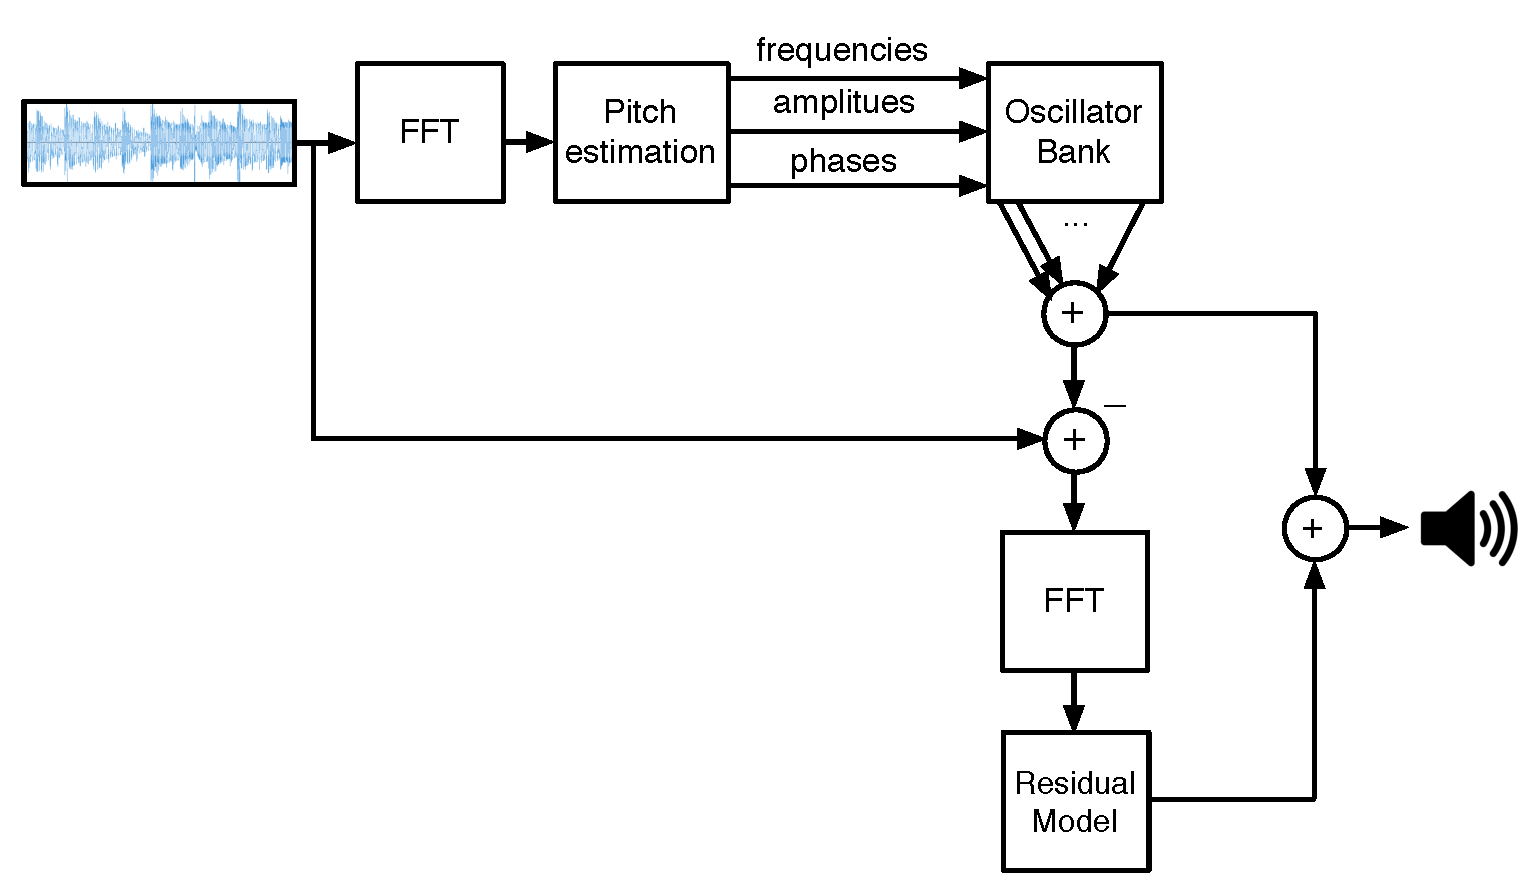
\includegraphics[scale=0.55]{SMS}
\caption[SMS]{Spectral modeling synthesis (SMS)}
\end{center}
\vspace{6pt}
\end{figure}
The deterministic portion contains sinusoids that are able to \newpage
\noindent change in frequency, via partial tracking methods, but as stated, these changes are represented by piecewise linear functions, which ``affects the generality of the model'' \cite[p. 31]{Tolonen:1998bh}. Transients are also difficult to model. This has led to the development of an extended technique called transient modeling synthesis (TMS), which ``provides a parametric representation of the transient components'' \cite[p. 33]{Tolonen:1998bh}. However, TMS requires the accurate segmentation of transients from a given signal, which is a difficult problem in its own, as discussed in \cite[p. 16]{Ciglar:2009uf}. \begin{singlespace}
\noindent Additionally, Serra and Smith note that:
\begin{quote}
%\linespread{1}
\selectfont
the characterization of a single sound by two different representations may cause problems. When different transformations are applied to each representation [which is common in order to transform the target sound], it is easy to create a sound in which the two components, deterministic and stochastic, do not fuse into a single entity \cite[p. 23]{Serra:1990dk}.
\end{quote}
%\linespread{1.7}
\selectfont
\end{singlespace}
Klingbeil adds that ``partial tracking becomes particularly difficult in the presence of noise, reverberation, or dense polyphony'' and also that SMS ``requires a number of input parameters [that] can have a significant effect on the quality of the analysis'' \cite[p. 42]{Klingbeil:2009lo}.

While there has been less work produced on re-synthesis methods that overlie physical models, and abstract algorithms like FM Synthesis, some interesting research has developed in the last decade.

Vercoe, Gardner and Scheirer point out that physical modeling (e.g. digital waveguide) parameter estimation ``has a particular advantage over equivalent estimation for additive, FM, or other abstract synthesis models in that the resulting parameter set has a clearly understandable interpretation, which aids in further signal manipulation'' \cite[p. 11]{Vercoe:1998hh}. This is due to physical modeling's low-dimensional and intuitive parameter set. Bensa, Gipouloux, and Kronland-Martinet estimate the parameters for a piano hammer-string model by analyzing a time-frequency representation of a recorded piano tone. Because the mapping of the time-frequency representation to the parameter values is complex, the authors used nonlinear optimization techniques---specifically simulated annealing, which will be discussed later---to search through the parameter space for the appropriate parameter set \cite[p. 499]{Bensa:2005xq}. A similar study was performed by Riionheimo, who used nonlinear optimization techniques to estimate the parameters of a plucked string physical model \cite{Riionheimo:2003qo}. Parameter estimation for physical models is a promising area of research for recreating the sounds that the models are designed for, but due to the high specificity of each model, these techniques will not be applicable outside of a small region of timbre space.

Techniques developed for re-synthesis based on frequency modulation are often referred to as \textit{adaptive-FM} or \textit{FM-matching} techniques (see Figure 13). 
\begin{figure}[h!]
\begin{center}
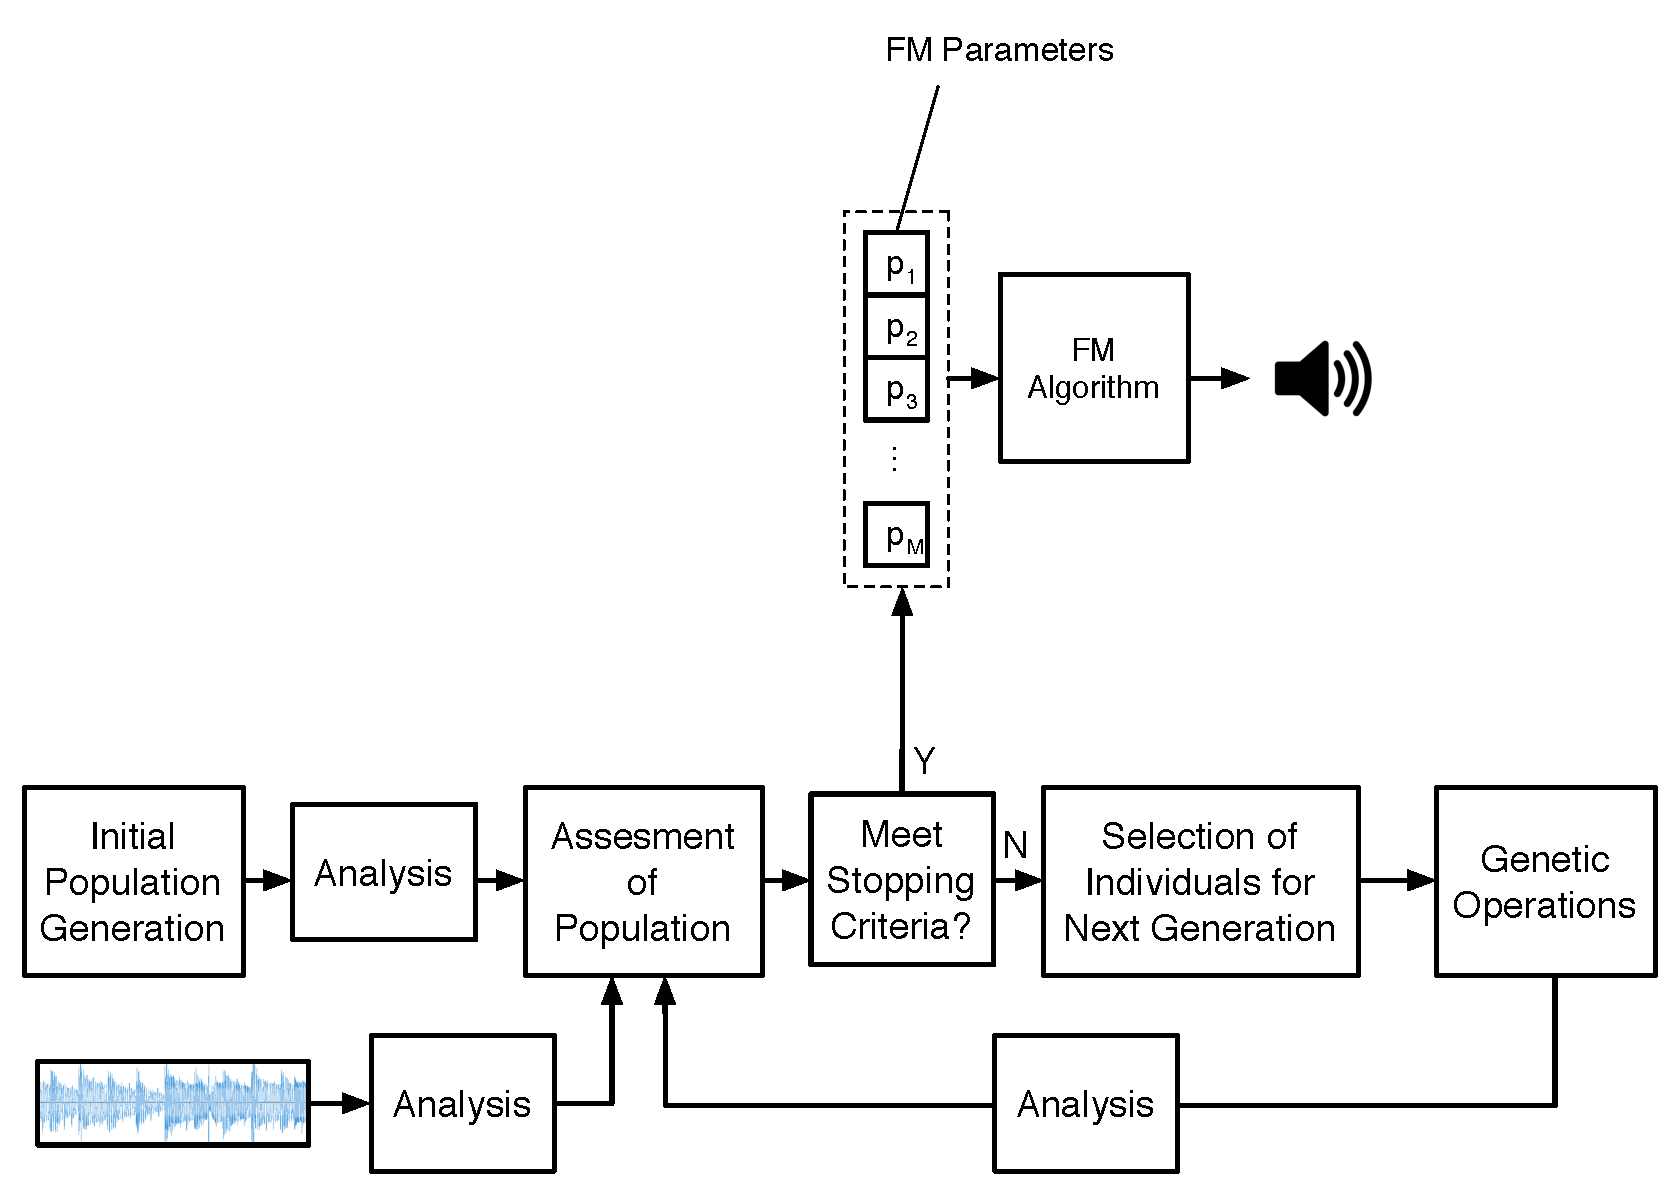
\includegraphics[scale=0.50]{AdaptiveFM}
\caption[Adaptive FM]{Adaptive FM using Genetic Algorithms}
\end{center}
\vspace{6pt}
\end{figure}
The first researchers to successfully re-synthesize sounds using FM Synthesis were Horner, Beauchamp, and Haken \cite{Horner:1993il}. Similar to physical modeling, the relationship between FM synthesis' parameter space and its output's time-frequency representation is unclear. Thus, Horner et al. also made use of a nonlinear optimization technique, a genetic algorithm (GA), to search for an optimal parameter set given a target. In these initial experiments, the parameters were not allowed to vary over time, limiting the applicability of the system \cite[p. 22]{Horner:1993il}. This system has been extended via a number of studies outlined by Horner \cite{Horner:2003ov}. 

One of the more successful FM-matching systems, developed by Mitchell and Sullivan, matches time-varying FM synthesis parameters to various complex sounds using GAs \cite{Mitchell:2005ez}. The FM topographies used were allowed to be more complex than one with a single modulator and carrier signal (e.g. the \textit{double modulator} design uses the sum of two modulators to vary the carrier signal's frequency). However, even complex FM topographies are well suited to only small regions of timbre space and so adaptive-FM techniques suffer from the same drawbacks that physical modeling re-synthesis does.
\vspace{12pt}
\section{Meta-Synthesis}

As noted, each re-synthesis technique mentioned is used to fit parameters to one specific synthesis algorithm and will inherit that algorithm's undesirable properties. In other words, as Garcia points out (and as reiterated by Tolonen \cite[p. 103]{Tolonen:1998bh}), ``it is known that different sound synthesis techniques perform better with different types of sounds'' \cite[p. 1]{Garcia:2001jw} and therefore, depending on the target sound, ``parameter matching techniques can give poor results when using a fixed topology'' \cite[p. 1]{Garcia:2000th}. We therefore expect any re-synthesis technique that rests on top of a single synthesis algorithm to be optimal for only certain types of sounds. One solution, as proposed by Misra and Cook \cite{Misra:2009km}, is to use a different synthesis algorithm (and consequently a different re-synthesis technique) for different kinds of sounds, so that each sound is generated by an algorithm that best suits it. Going forward, we refer to this approach as meta-synthesis (see Figure 14) \cite[p. 1]{Misra:2009km}. 
\begin{figure}[h!]
\begin{center}
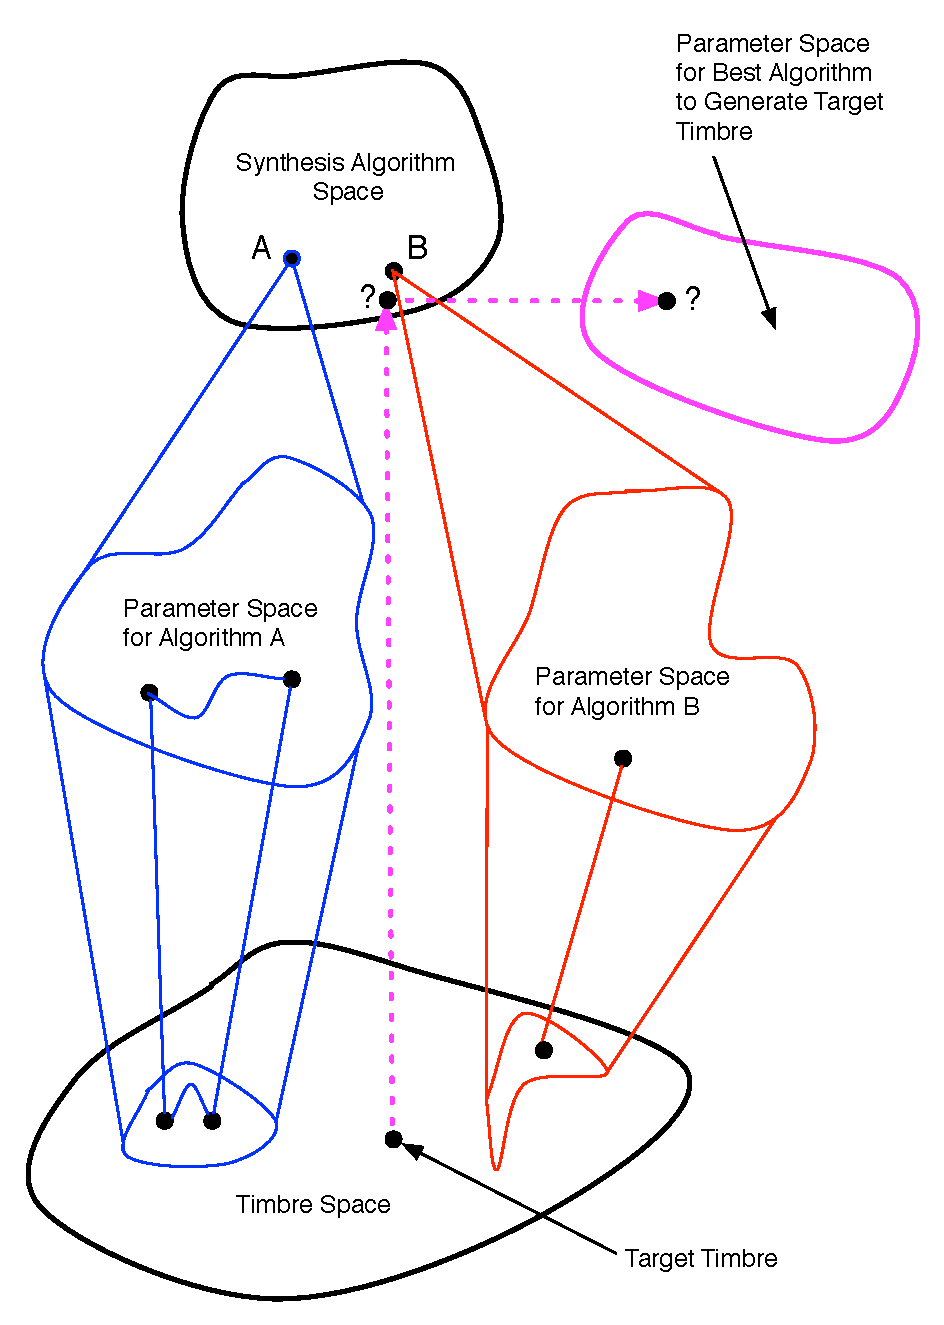
\includegraphics[scale=0.70]{MetaSynthesis1}
\caption[The meta-synthesis problem]{The Meta-Synthesis problem}
\end{center}
\vspace{6pt}
\end{figure}
Knowing which algorithm to choose is often not obvious and, therefore, placing the burden of this choice on the composer is not ideal. In their concluding comments, directly related to this issue, Misra and Cook write that a way to relieve this burden would be to ``present the entire range of [synthesis] techniques to the machine and let it decide which to use on-the-fly''  \cite[p. 5]{Misra:2009km}. Such a system would require the machine to \textit{learn} which synthesis algorithms (and therefore also which re-synthesis techniques) are best suited for which kinds of sounds. However designed, the learning machine used would have to be trained on enough timbral data to sufficiently blanket timbre space. Also, one must develop a metric by which to measure how \textit{suited} each algorithm is for each sound, so that one may be assigned the \textit{winner}. If such a process were possible, a \textit{winner} could be determined for each individual point in timbre space, leading to an association between common synthesis algorithms and the timbre space regions within which they are most suitable. However, the issues of generating sufficient training data and measuring suitability of not just the synthesis algorithm, but also its paired re-synthesis technique (for a given point in timbre space) are not trivial.

Instead of having to generate and provide enough timbral data to blanket timbre space, Puckette's research into re-synthesis provides an alternative method that could also be used when designing a meta-synthesis system (see Figure 15) \cite{Puckette:2004zp}.
\begin{figure}[h!]
\begin{center}
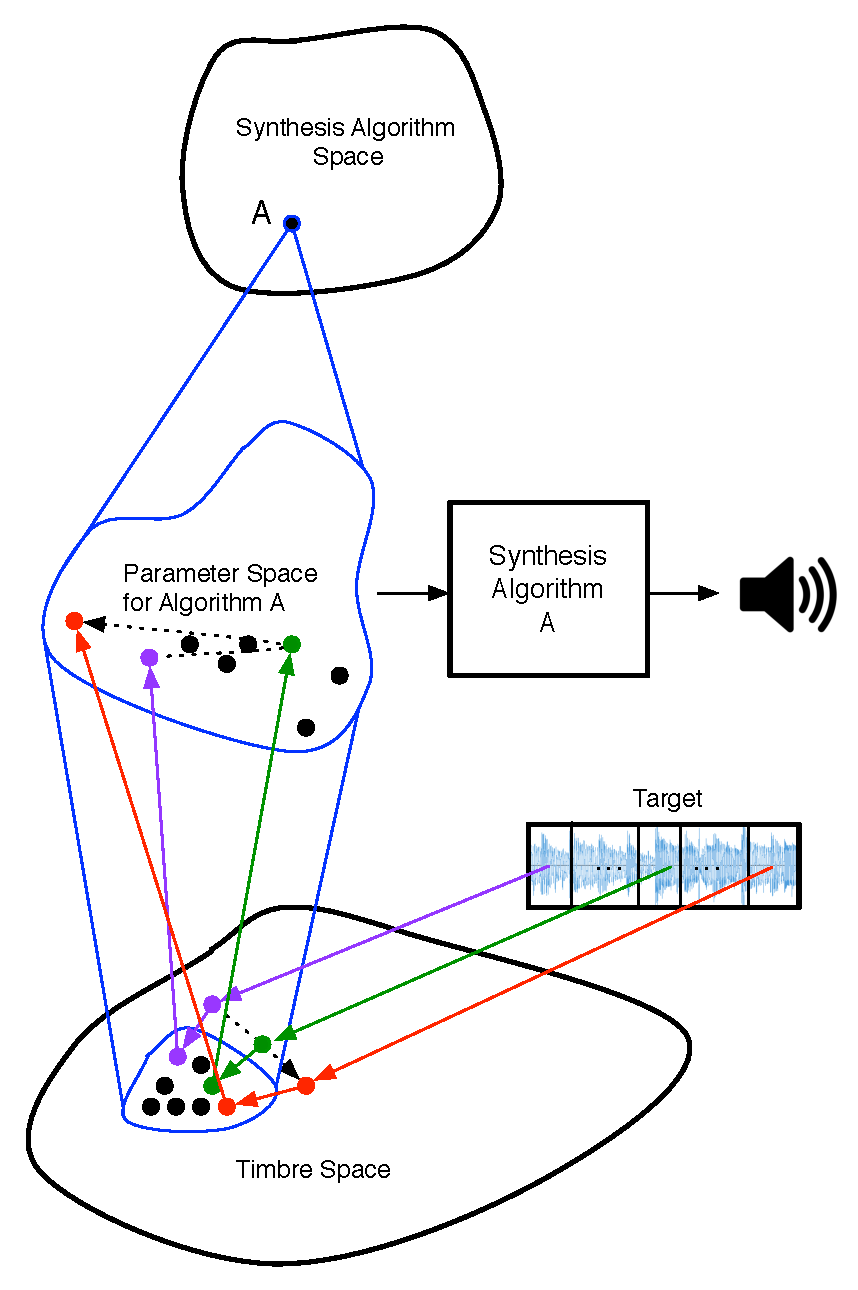
\includegraphics[scale=0.75]{PucketteMetaSynthesis}
\caption[Mapping timbre to parameters]{Finding the closest parameter mappings in a partially canvassed objective timbre space.}
\end{center}
\vspace{6pt}
\end{figure}

First, the author defines an 11-dimensional objective timbre space by segmenting a spectrum's magnitude into 11 bands, calculating the loudness in each, and then transforming the result into a vector whose values are uncorrelated \cite[p. 1-2]{Puckette:2004zp}. He then uses a specific synthesizer to generate points in this timbre space by 
\clearpage
\noindent sufficiently blanketing the input parameter space. When a target sound - corresponding to a path in the timbre space - is provided to his system, it re-synthesizes the sound by finding the synthesizer's nearest neighbors (using Euclidean distance) to each point in the target path, determining the \textit{smoothest} trajectory through these nearest neighbors, and mapping this trajectory back to parameter space to determine how the synthesis algorithm can best produce the target \cite[p. 3]{Puckette:2004zp}. 

Puckette notes that since his system was initially produced to force a specific synthesizer to produce the target, there may be no nearby synthesis points to the target curve \cite[p. 3]{Puckette:2004zp}. However, one could easily extend Puckette's system by using a number of different synthesizers to produce points in timbre space and then, for a given target, constrain the match trajectory to pass only through points of one synthesizer, so that the resultant parameter set would correspond to the synthesizer which \textit{best fits} the target. 

This extended version of Puckette's system would also separate the suitability of the synthesis algorithm from its specific re-synthesis technique, because the re-synthesis process would be the same for all synthesis methods. Therefore, the proposed extended version of Puckette's system would solve many of the issues previously posed when developing a learning machine able to intelligently choose between synthesis algorithms. However, it is not without its own set of problems. First, it is not clear that euclidean distances in Puckette's objective timbre space are semantically meaningful. Second, there is no indication for when one has sufficiently blanketed the input parameter space of a given synthesizer. Third, a smooth trajectory of points in timbre space does not necessarily lead to a smooth trajectory to points in the parameter space. Since trajectories are drawn through a finite set of points in the timbre space, one must determine how best to interpolate between parameter sets in the input space, which, depending on the mapping, could produce wild fluctuations between the points back in timbre space. Fourth, no matter how many synthesizers are provided to the system, it is not guaranteed that all points that are mapped from the various parameter spaces to this timbre space will have close neighbors, making parameter interpolation errors even more apparent when such points are chosen to contribute to the optimal trajectory. Lastly, it is not necessarily the case that the match trajectory will correspond to the \textit{best suited} synthesis algorithm, because many algorithms have high-dimensional and non-intuitive parameter spaces, and therefore, while they may provide a best fit to the target trajectory, they may also present a more complicated exploration than another algorithm with the next best fit.

Loviscach's work on making synthesizer control feel more natural for synthesizers with large parameter spaces provides a solution to this last problem \cite{Loviscach:2009mi}. In his work, Loviscach studies correlations between parameter sets for a given synthesizer based on a database of preset data. If two different parameters are highly correlated over a broad range of parameter presets, then adjusting one will adjust the other \cite[p. 1]{Loviscach:2009mi}. Correlations are found between all pairs of parameters and placed in a two-dimensional field such that highly correlated parameters are placed next to each other. The manipulation of any one parameter will affect all others according to their distance and joint statistics \cite[p. 1]{Loviscach:2009mi}. Thus, assuming that the provided presets for a given synthesizer correspond to a synthesizers natural usage, this system is able to replace a synthesizer's high-dimensional non-intuitive parameter space with a more natural low-dimensional one. Of course, this requires that enough presets exist for each synthesizer so that their parameter correlations can be considered statistically significant. In this case, however, a hybrid system employing techniques from both Puckette's and Loviscach's research could be quite interesting. The major hurdle would be having the enormous amount of training data necessary for both techniques to work well in harmony, making such a system impractical. In theory, however, this hybrid system would allow a composer to provide a target timbre and, in return, they would be given a specific algorithm and parameter set that they could then use to explore the surrounding space in a natural way. If further constraints are placed on storage and efficiency, this system would meet the basic requirements of an ideal synthesis tool. However, other authors have suggested that one could do even better than this.

A limitation of the synthesis learning machine that is suggested by Misra and Cook (an example of which is outlined above as an extension of both Puckette's and Loviscach's work) is that it is only able to choose from a finite set of synthesis topologies when selecting a best-fit topology and corresponding parameter set \cite[p. 1]{Misra:2009km}. Suggested as early as 1998 by Vercoe, Gardner and Scheirer and supported by Garcia \cite[p. 2]{Garcia:2000th} and Moreno \cite[p. 1]{Moreno:2005bs}, hybrid synthesis methods - those allowing any combination of the \textit{classical methods} - can provide better solutions to imitative sound synthesis both perceptually and in matters involving controllability \cite[p. 9]{Vercoe:1998hh}.

The research of Carpentier, Tardieu, Harvey, Assayag, and Saint-James exploits this same well-known fact in the domain of acoustic orchestration \cite{Carpentier:2010fh}. They use acoustic instruments as their \textit{synthesis methods} and allow any realistic linear combination of these instruments to generate a given target (see Figure 16). 
\begin{figure}[h!]
\begin{center}
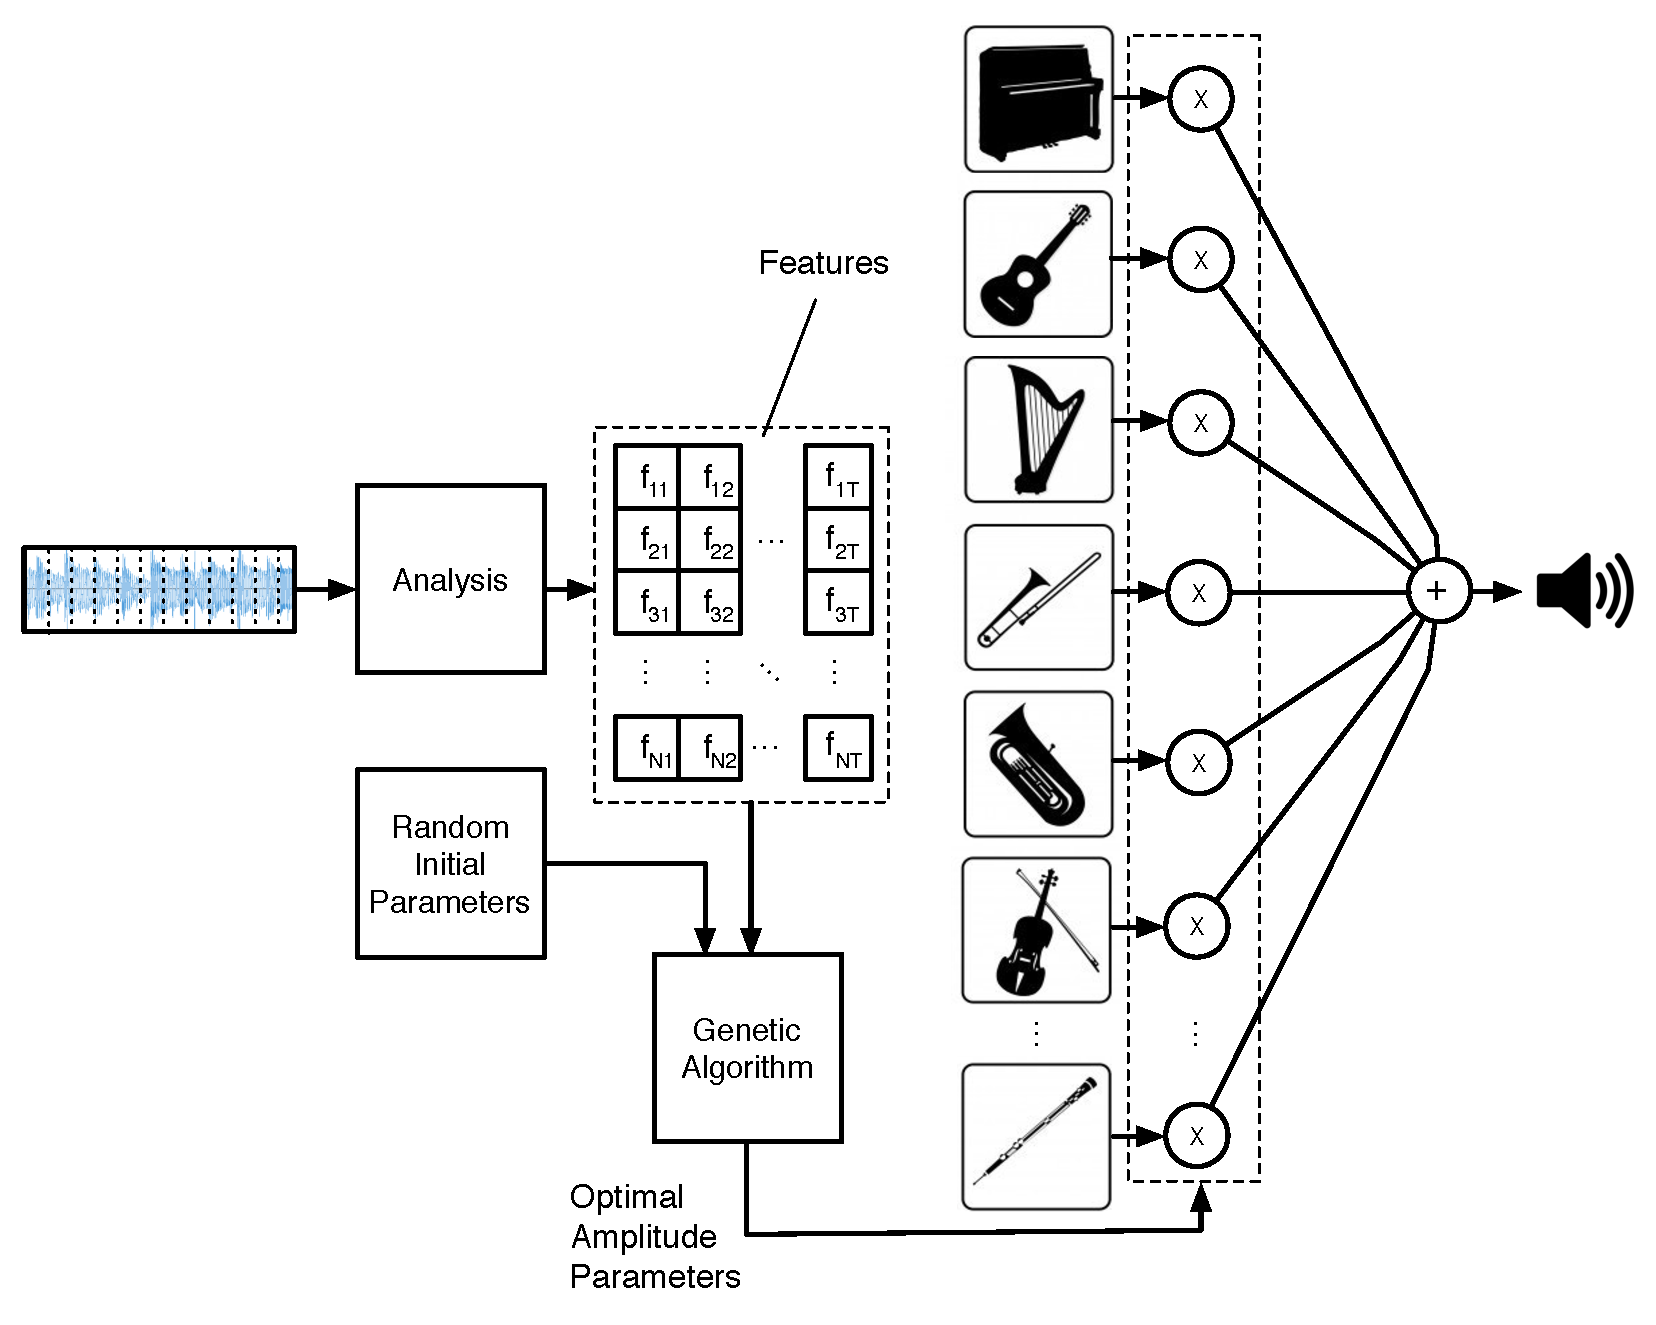
\includegraphics[scale=0.55]{OrchestralMetaSynthesis}
\caption[Searching for linear combinations of orchestral instruments]{Approximating a complex timbre using a linear combination of orchestral instrumentation.}
\end{center}
\vspace{6pt}
\end{figure}
The re-synthesis problem becomes more difficult than simple parameter fitting for fixed topologies, because there is a combinatorial explosion in the number of topologies available. In order to determine an appropriate combination of instruments and associated playing techniques, they map individual instrument features (obtained from steady-state time-frequency representations) to an objective timbre space, make assumptions about how these features interact in the presence of polyphony, and perform a search over all possible combinations for that which best achieves the target \cite[p. 2]{Carpentier:2010fh}. The authors limit their system to steady-state sounds and suggest that a way to transition between timbres is to do so incrementally, with one instrument dropping out or modifying its state at a time. Such transitions would be limited in how \textit{smooth} one perceives them to be as well as how quickly they may occur. However, one may be able to avoid this problem when designing a system that utilizes the same basic idea, but is based on linear combinations of synthesis algorithms as opposed to combinations of acoustic orchestral instruments.

There are a few other constraints that Carpentier et al. faced that would not be necessary when designing similar systems that utilize linear combinations of synthesis algorithms. First, Carpentier et al. designed their system specifically as an auto-orchestration mechanism for given target sounds, constraining their search to a realizable orchestral combination \cite{Carpentier:2010fh}. This constraint need not be applied when combining sound synthesis algorithms. Also, It is not necessary to consider typical sound synthesis algorithms as \textit{atomic} units, as it is in the acoustic instrument case. By removing this limitation, one may be able to generate better-suited synthesis algorithms for a given target using building blocks at a different level of abstraction. Replacing high-level blocks with the lower-level components that make them up, one would be able to generate solutions at least as fit as any of those generated using the higher-level set, and possibly better \cite[p. 2]{Garcia:2000th}. However, the search space becomes larger as the atoms become lower-level and, therefore, the search itself becomes more difficult. Thus, one must balance the theoretical ability of the system to produce possibly better solutions with the practicality of being able to find one of these solutions. 

A few studies have attempted to build a system capable of constructing synthesis algorithms, well-suited to a given target, via an intelligent, directed search through synthesis algorithm space \cite{Wehn:1998bh, Garcia:2000th, Garcia:2002cq}. Before being able to discuss this research in any detail, one must familiarize themselves with the underlying search strategy both studies employ as well as understand why it is optimal for this task.
\vspace{12pt}
\subsection{Searching for Synthesis Algorithms}
An exhaustive search over synthesis space is not possible, no matter how large the atomic topology unit. Even when this search is restricted over one single topology, the parameter space will often be enormous. Therefore, it is necessary to investigate intelligent ways of searching such a high-dimensional and complex space. In order to develop a directed search technique, one must consider a way to measure how well each point in the input space performs at the given task. The resultant measure is typically represented by an \textit{objective function} that, given a point in the input space, produces a value (often between $0.0$ and $1.0$) that represents how well the point meets the target objective. The optimal solution to the problem will exist as a global maximum along the objective function's surface (see Figure 17). 
\begin{figure}[h!]
\vspace{24pt}
\begin{center}
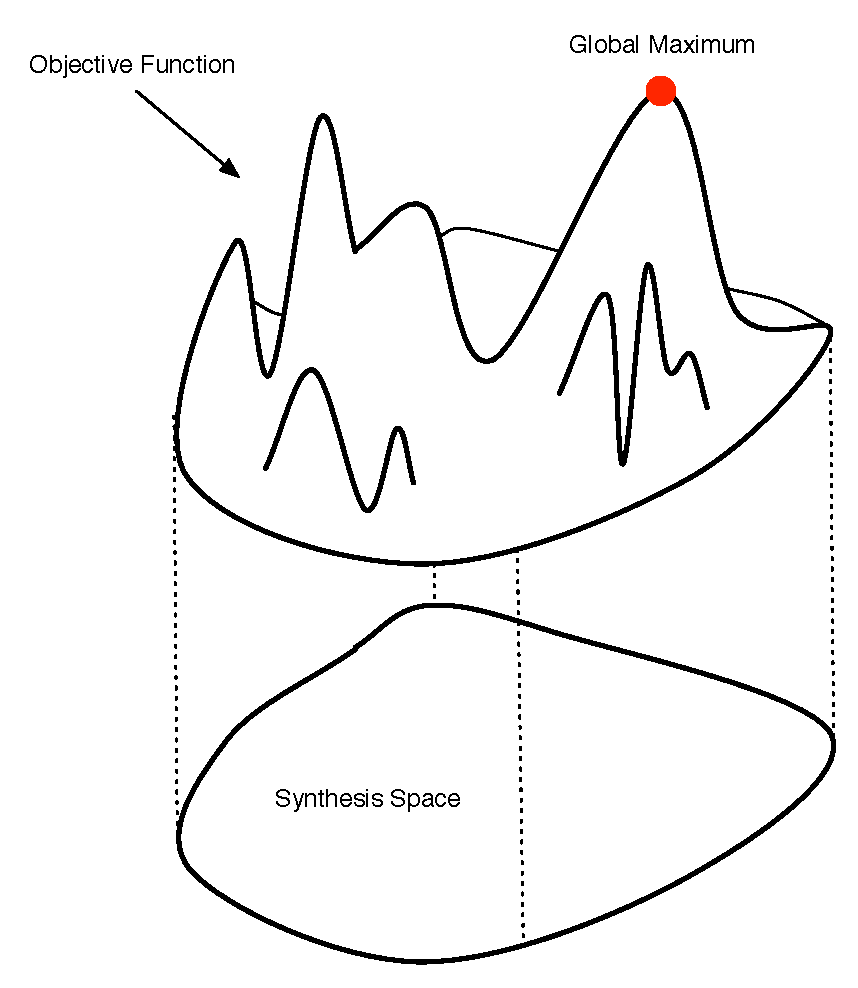
\includegraphics[scale=0.7]{FitnessFunction}
\caption[Fitness function]{An objective function/surface sitting above synthesis space with its global maximum shown.}
\end{center}
\vspace{6pt}
\end{figure}
The closed-form representation of this function is often unknown, making search difficult. However, in some cases, one can make reasonable claims about the shape of the objective surface.

The artificial intelligence community has developed various intelligent search algorithms to address such problems, which direct the search based on hypotheses about the objective surface's shape (see Figure 18), and/or restrict the region of search based on known characteristics of the desired solution \cite[p. 64-108]{Russell:2009ai}.
\begin{figure}[h!]
\begin{center}
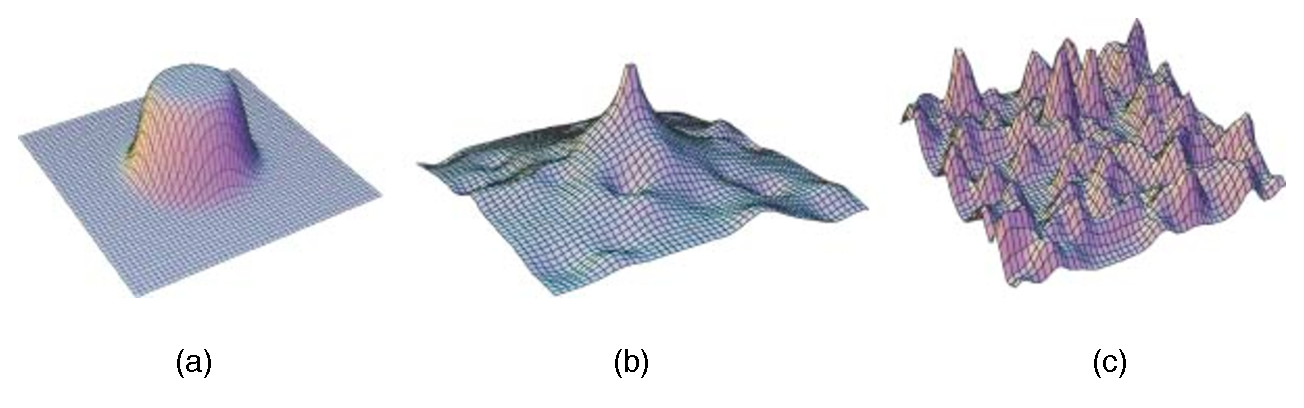
\includegraphics[scale=0.6]{DifferentTopologies}
\caption[Fitness surface topologies]{Three different fitness surfaces: (a) unimodal and smooth, (b) multimodal, but relatively smooth and with a clear global maximum, and (c) multimodal and rough with no clear global maximum.}
\end{center}
\vspace{6pt}
\end{figure}

If one can assume that the objective surface is unimodal and smooth, then the most efficient search algorithm is called hill-climbing, which simply looks at all neighbors of the current position in the search and moves in the direction of greatest increase in the objective function. However, if the surface is not unimodal, then this algorithm has a chance of converging to a local maximum, which is undesirable. Teller writes that hill-climbing is a fully-exploitative search algorithm, meaning it ``focuses the search in the areas of the search space that have the highest known [objective] values'' \cite[p. 23]{Teller:1998ly}. He explains that ``in search there is sometimes a trade-off between exploration and exploitation'' whereas opposed to exploitation, ``exploration means trying out options that are believed to be locally sub-optimal (in hopes that globally these options will lead to an improved solution)'' \cite[p. 23]{Teller:1998ly}. If no assumptions about the shape of the objective surface can be made, then one must find a good balance between the exploitation and exploration in search so that premature convergence is unlikely to occur. Search strategies with this balance are often employed---and are known to be most productive---in cases where the problem domain is not well understood, and one does not know a priori about the structure of the solution, as is the case with the synthesis problem that we are facing \cite[p. 42]{Vanneschi:2004le}. Thus, it is not a coincidence that variants of genetic algorithms (GA)---a strategy that provides mechanisms to directly control the amounts of exploitation and exploration---have been successfully utilized in many of the parameter estimation studies listed above \cite{Horner:1993il, Johnson:1998sh, Mitchell:2005ez, Riionheimo:2003qo}. The degree to which GAs have helped solve the FM matching problem has led Horner, one of the initial pioneers of FM matching, to proclaim that it has helped push FM matching ``into something of a renaissance period'' \cite[p. 28]{Horner:2003ov}.

As described in his dissertation on making variants of GAs more efficient, Vanneschi writes that GAs ``can be imagined as operating via a population of explorers initially scattered at random across the landscape. Those explorers that have found relatively high fitness points are rewarded with a high probability of surviving and reproducing'' \cite[p. 70]{Vanneschi:2004le}. (When discussing GAs, the objective surface is often referred to as the \textit{fitness} surface and the process of search is called \textit{evolution}.) The \textit{pull} strength of explorers from regions with low fitness values to regions with high fitness values is determined by the GA's parameters, allowing one to specify in what ways the algorithm exploits and explores. The ability to search many different regions of the input space in parallel increases the probability of finding many local optima on a complex multi-modal fitness surface and then selecting the best option between all of them \cite[p. 37]{Garcia:2001jw}. For a visual example of how a GA might obtain a near-optimal parameter set, see Figure 19.
\begin{figure}[h!]
\vspace{24pt}
\begin{center}
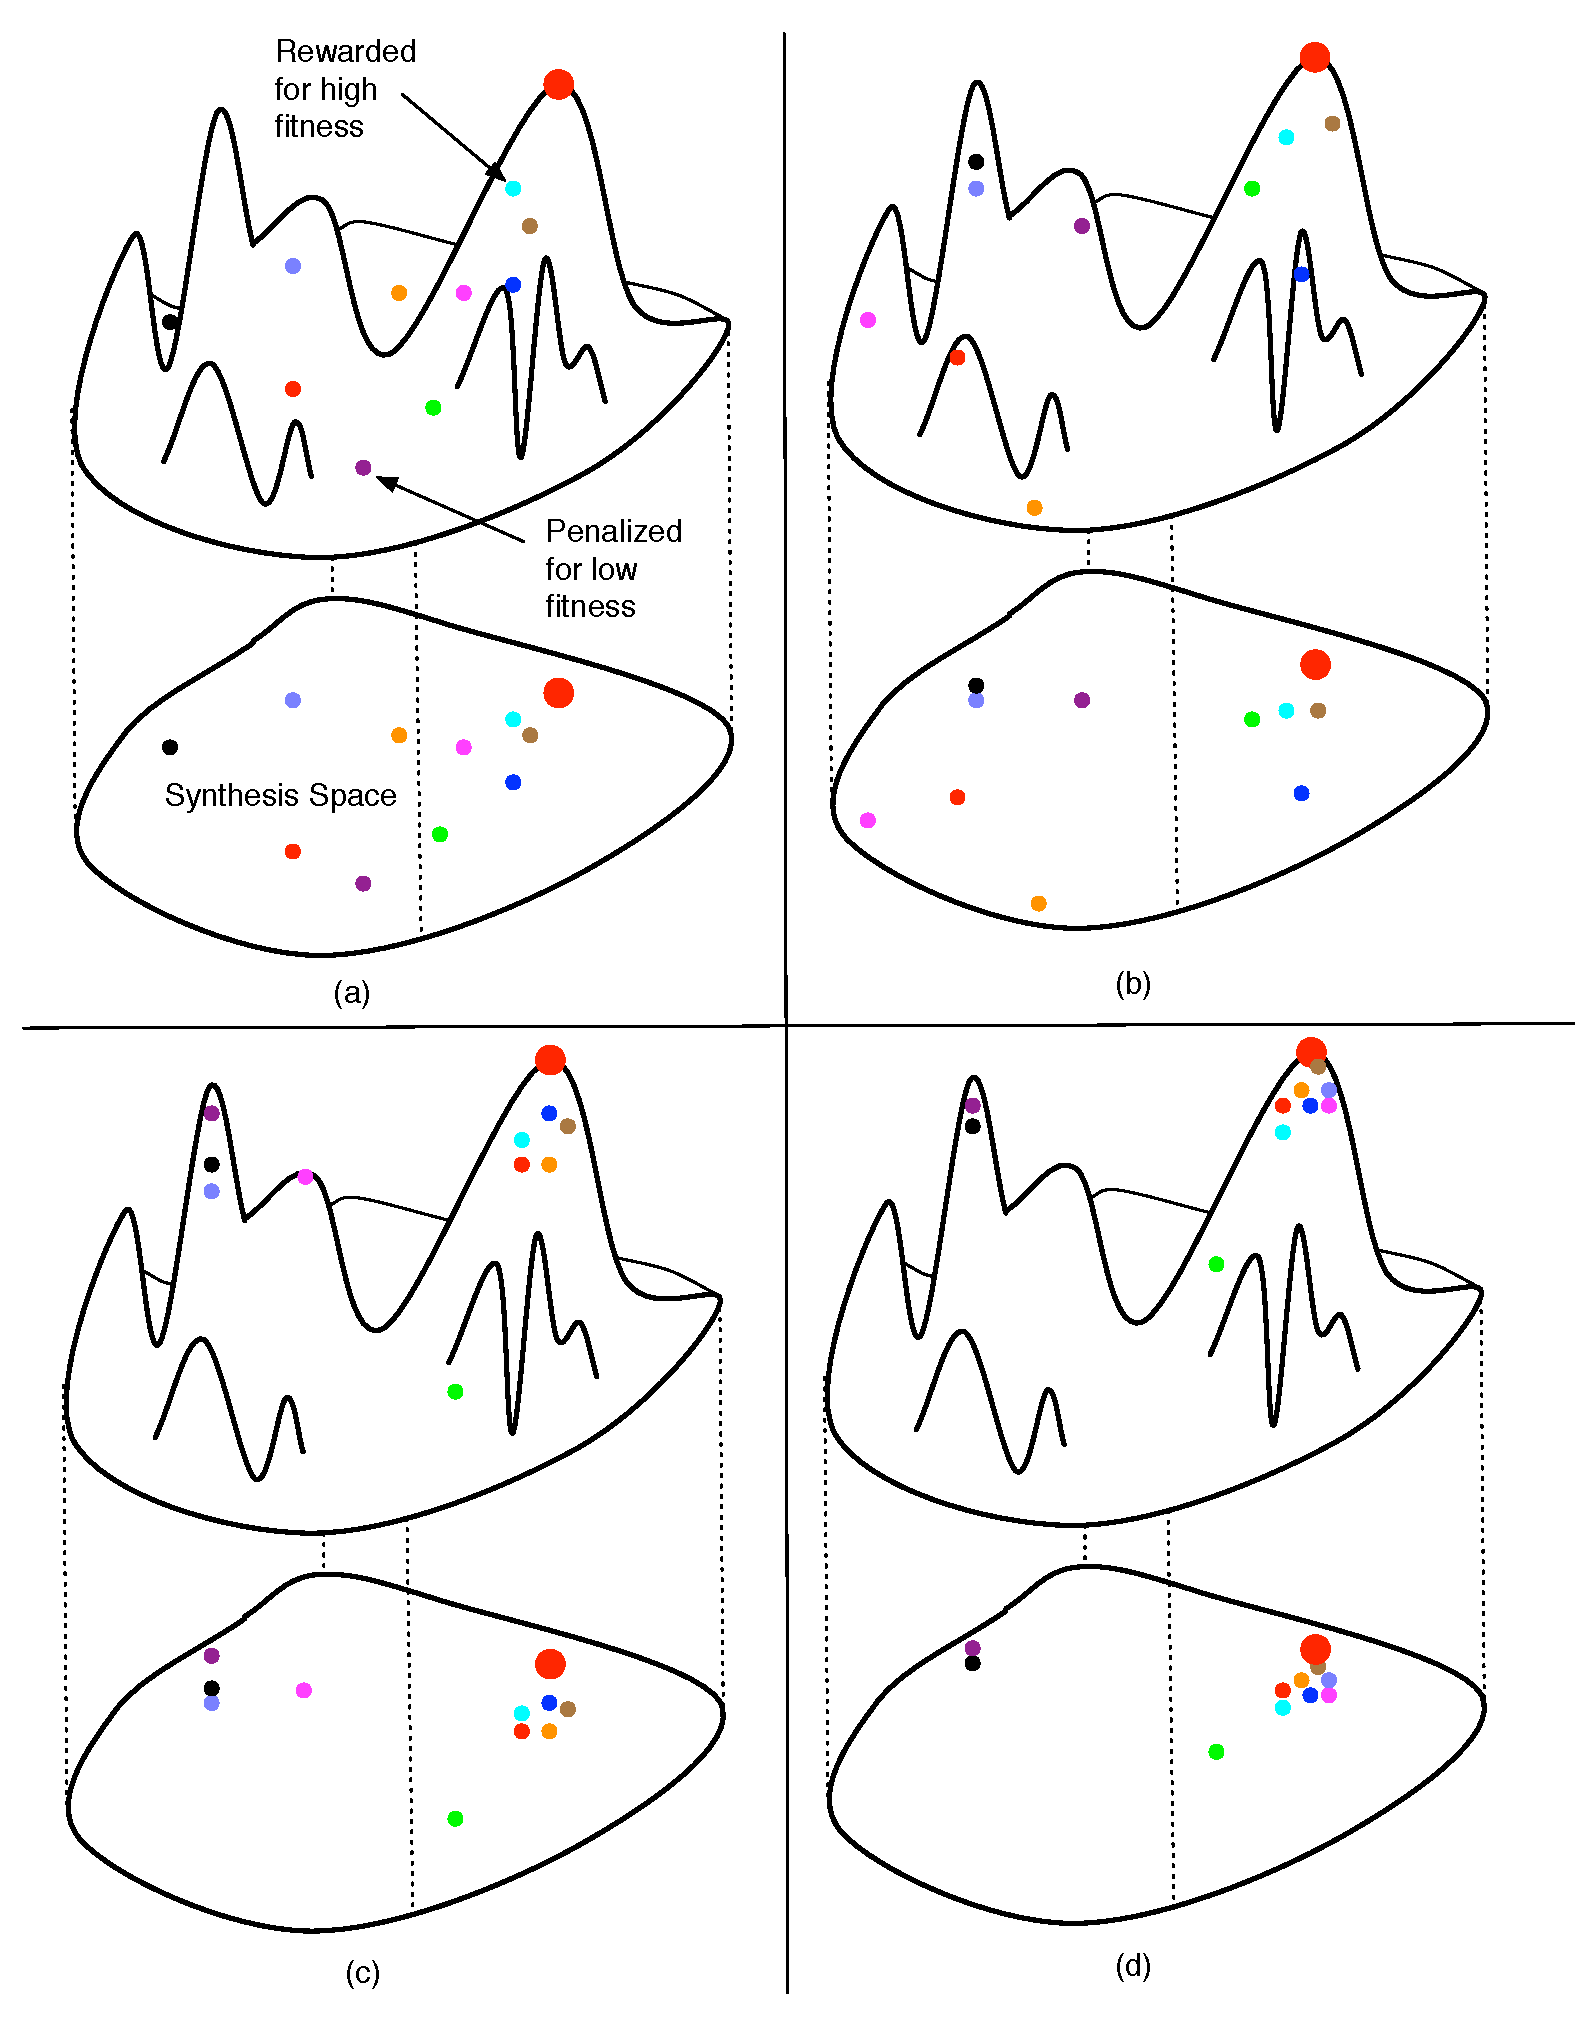
\includegraphics[scale=0.50]{GASearch}
\caption[GA example]{A GA population after: (a) $1$, (b) $10$ (c) $100$, and (d) $1000$ iterations (and optimal solution notated by large red dot).}
\end{center}
\vspace{6pt}
\end{figure}

Since it is known that for at least several fixed topology parameter estimation techniques (e.g. FM matching, physical model parameter estimation, granular re-synthesis), the objective surfaces are best searched via genetic algorithms, it is very likely that the objective surface for the more complex problem of simultaneous topology and parameter estimation will also be best searched using genetic algorithms. However, classical genetic algorithms can only be applied when the size and shape of the solution is known beforehand \cite[p. 42]{Vanneschi:2004le}. In the search for an appropriate synthesis algorithm topology, the size and shape of the ultimate solution is a large part of the problem and so classical GAs will not work. Instead, one must look to automatic programming research---the area of study dedicated to designing more sophisticated search methods that are specifically suited to work in algorithm space---to find more appropriate search algorithms for this task.

``Automatic Programming is one of the central goals of computer science...[which is to make] computers perform required tasks without being told explicitly how to accomplish these tasks'' \cite[p.3]{Koza:1997zr}. Ideally, in an Automatic Programming system, requirements provided by the user only specify what the intended behavior of the program is and not how it should produce that behavior. In a paper overviewing the many different approaches to Automatic Programming, Rich and Waters \cite{Rich:1992sp} state that Automatic Programming has three goals: to make a system end-user oriented, general purpose, and fully automated \cite[p. 4]{Rich:1992sp}. All approaches in existence at that time focused on two of these goals at the expense of the third. Rich and Waters split these approaches into three categories: bottom-up, narrow-domain, and assistant \cite[p. 3]{Rich:1992sp}. Bottom-up approaches sacrifice the user-oriented goal and result in high-level programming languages that are general purpose and fully automated (i.e. they automatically generate machine code), with a goal of becoming ``very high level in the future'' \cite[p. 3]{Rich:1992sp}. Narrow-domain approaches focus on a narrow domain, but are end-user oriented and fully automated, with the goal of becoming wider-domain in the future \cite[p. 4]{Rich:1992sp}. The assistant approaches lead to systems that are user-oriented and general purpose, but not fully automated (e.g. integrated development environments (IDEs)) \cite[p. 4]{Rich:1992sp}. 

The meta-synthesis problem suggests the need for a narrow-domain system (only designed for generating synthesis algorithms) that is end-user oriented (where the end user only needs to specify a target output) and fully automated (the synthesis topology and optimal parameter set are found and returned). These approaches typically frame the Automatic Programming problem as one of intelligently searching through algorithm space in order to find an algorithm able to produce the desired output, which is consistent with how we interpret the meta-synthesis task. The most common intelligent search strategy through algorithm space is, unsurprisingly, based on genetic algorithms and is called genetic programming (GP) \cite{Koza:1992gp}. In fact, genetic programming is so ubiquitous in Automatic Programming research that da Silva---in his dissertation on GP---mistakenly defines GP \textit{as} ``the automated learning of computer programs'' even though it is actually a subset of Automatic Programming \cite[p. ix]{Silva:2008le}.

GP can be thought of as ``variable length, tree-based genetic algorithms'' \cite[p. 29]{Teller:1998ly}. The search mechanics of GP are analogous to those of GAs, meaning GP also performs a parallel search through the input space for points (i.e. algorithms and paired parameter values) that meet the specified goal as measured by an appropriate fitness function (applied to an algorithm's output), balancing exploration and exploitation in a similar manner. The individual points in algorithm space are typically represented by tree data structures whose terminal nodes (also referred to as \textit{leaves}) represent input parameters to the other functional node elements (see Figure 20). 
\begin{figure}[h!]
\vspace{24pt}
\begin{center}
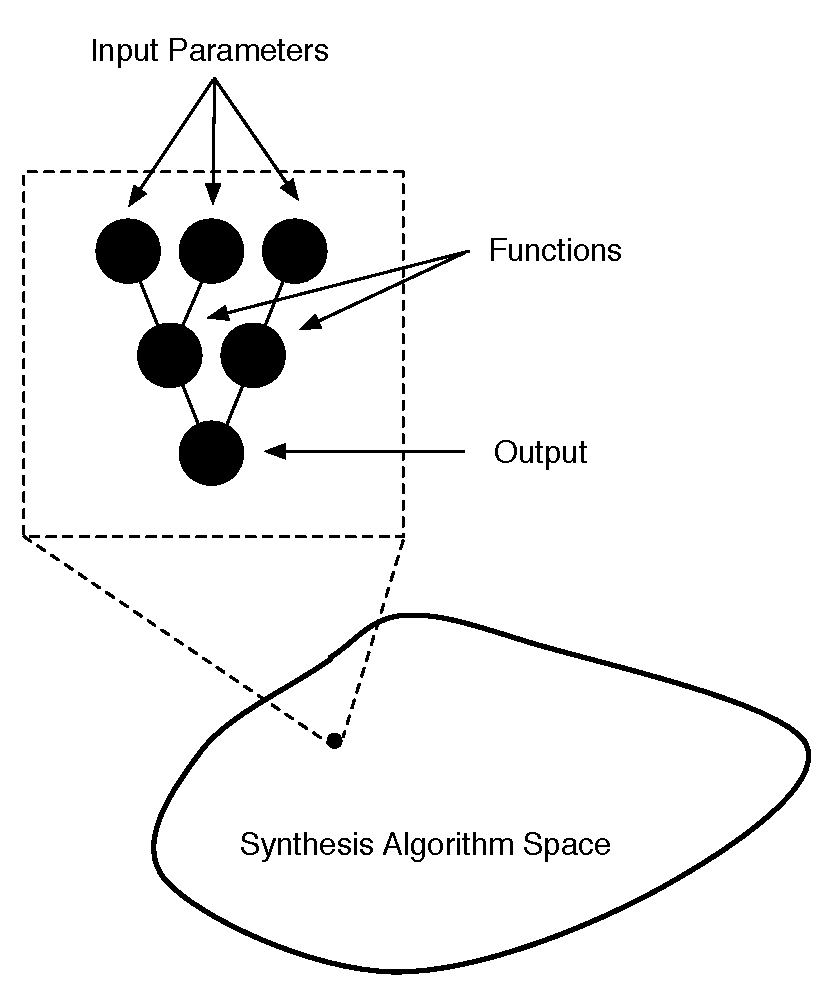
\includegraphics[scale=0.70]{GraphAsPoint}
\caption[The genetic programming paradigm]{The common Genetic Programming (GP) setup, where a point in algorithm space is represented by a tree.}
\end{center}
\vspace{6pt}
\end{figure}
This representation was first proposed by Koza as a natural way to structure Lisp programs \cite{Koza:1992gp}. It has been successfully applied to a number of different programming languages since. However, there are a number of different ways to translate code to this representation as well as a number of operator variants  used to perform the search, and as pointed out by Vanneschi, ``the art of choosing an appropriate representation and an appropriate set of operators is often a matter of experience and intuition'' \cite[p. 6]{Vanneschi:2004le}. Beyond choosing the representation and operators, there are also a number of GP parameters that must be set, and ``much of what GP researchers know about these parameters is [also] empirical and based on experience'' \cite[p. 32]{Vanneschi:2004le}. Progress on systematic ways of selecting specific orientations of these variables has been made recently and is further discussed in Chapter III - Approach.

There has been relatively little research into genetic programming in the arts compared to the hard sciences (e.g. robotics, circuit design) (Hollady \& Robbins, 2007, p. 1). However, there is no inherent reason why this should be the case. In their paper on human-machine interaction, Moroni, von Zuben, and Manzolli note that ``human-machine interaction in the context of artistic domains [can be] a framework for exploring creativity and producing results that could not be obtained without such interaction'' \cite[p. 185]{Moroni:2002oa}. It is certainly true that a meta-synthesizer would be able to provide a composer with the means to experiment with timbre in ways they would not be able to without it, thus leading them to places of creativity that they would not have been able to explore on their own. However, the first uses of GP in the artistic domain that predated any work on evolving synthesis algorithms were for evolving music-making systems---see \cite{Rowe:NoRead, Spector:1994ij, Johanson:1997gf, Polito:1997ly, Todd:1998tg, Costelloe:2007bv}.

As work in GP was being carried out in the music world, there were also advancements in GP for use in signal processing applications not related to music---see \cite{Sharman:1995bs, Alcazar:1997ve, Koza:1997zr, Miller:1998zr, Uesaka:2000jw, Holladay:2007ct}.

A signal processing application of GP that has implications for music as well is automatic feature extraction for various classification tasks. This was predated by GP work on video feature extraction \cite{Harris:1997qf, Teller:1998ly}. 

The first GP system to evolve audio feature extractors was proposed by Conrads, Nordin, and Banzhaf \cite{Conrads:1998wb}. They used machine-code level GP to extract features for vowel and consonant detection. 

Pachet and Roy also used GP to evolve feature extractors for classification tasks \cite{Pachet:2007if}. However, their function set contained much more complicated functions than the work of Conrads et al. Among some of the most complex functions were the Mel-frequency cepstral coefficient (MFCC) calculation, the fast Fourier transform (FFT), and the application of a high-pass filter. Their work was recently extended separately by Kobayashi and Vatolkin, Theimer, and Rudolph \cite{Kobayashi:2009la, Vatolkin:2009bd}.

Taking into account the Automatic Programming research carried out in both digital signal processing and in music composition over the last fifteen years, one may assume that a good amount of research has also been performed in evolving sound synthesis algorithms. However, this is not the case.

There have been a few studies involving sound synthesis evolution using Interactive-GP (where fitness measurements are provided by test subjects) for timbre exploration \cite{Dahlstedt:2001dd, Mandelis:2005iw, McDermott:2006gd}. However, while each study provides a system that is applicable to any kind of synthesis topology, a fixed topology is chosen for each run of the system. As previously noted, making the user choose a fixed synthesis topology at the beginning of a run can severely limit the regions of timbre space that are even possible to explore. Additionally, using subjective judgements to steer the search requires that the user stay actively involved during the length of the search. A more desirable solution would replace the need for human fitness evaluation with an objective measure that correlates well. This would require the development of an objective timbre space wherein distances are semantically meaningful, so that pairwise similarity tests could be performed by the computer in order to replace subjective assessment by the end-user.

Wehn was the first researcher to investigate such a system \cite{Wehn:1998bh}. A high-level diagram of his system can be found in Figure 21.
\begin{figure}[h!]
\vspace{24pt}
\begin{center}
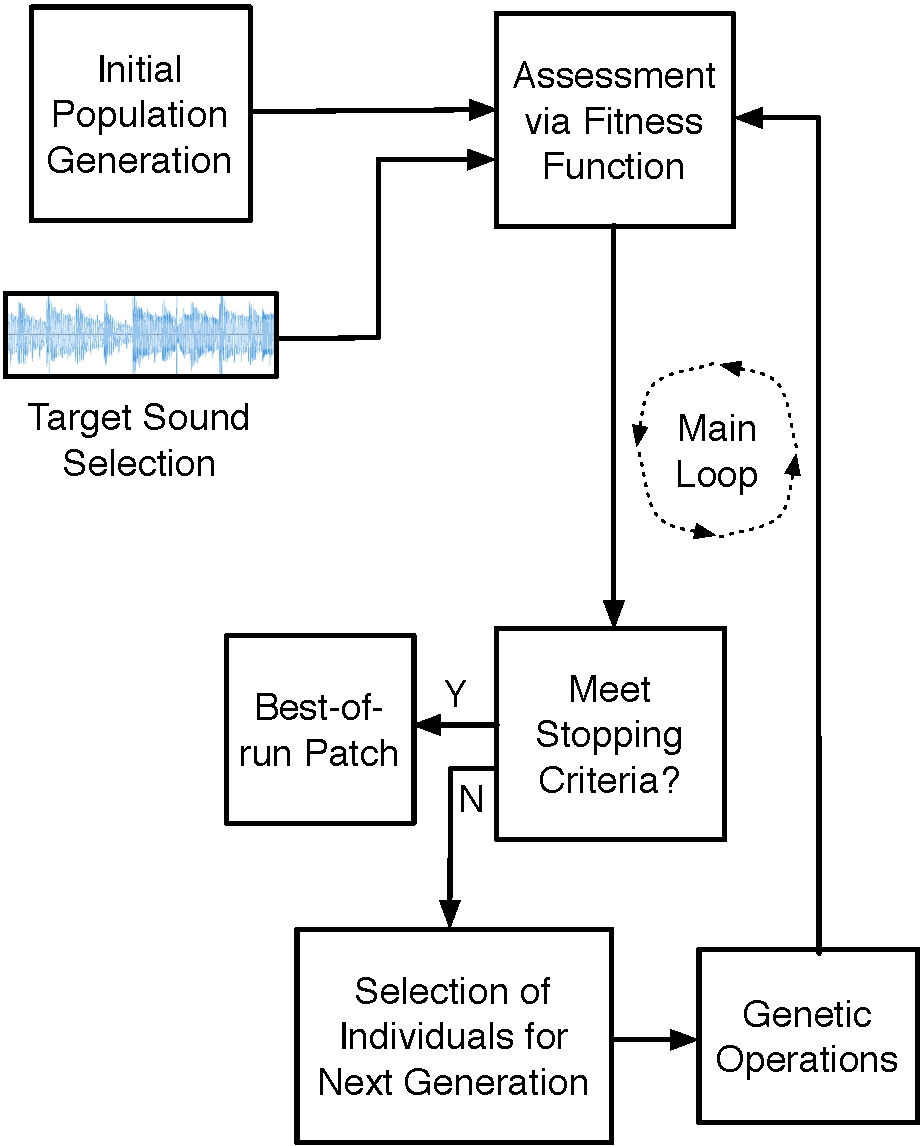
\includegraphics[scale = 0.6]{SimpleSystem}
\caption[GP for sound synthesis]{A high-level overview of using GP for generating synthesis algorithms.}
\end{center}
\vspace{6pt}
\end{figure}
In his work, he uses a basic \clearpage
\noindent function set comprised of noise, steady-state sinusoids, triangle and square waves, ramp functions, addition, multiplication, and high, low, and bandpass filters from which to generate more complex algorithms \cite[p. 2]{Wehn:1998bh}. The target sounds that Wehn tests his system with do not vary in time and he does not provide a mechanism by which time-varying sounds can be generated, but as a first step towards our goal, his work is important.

In order to assess fitness, Wehn calculates the Euclidean distance between the amplitude spectra of a target sound and those produced by the synthesizer output \cite[p. 2]{Wehn:1998bh}. Thus, Wehn implicitly assumes a timbre space where each point is represented by the elements of a magnitude spectrum. This is a problematic assumption for many reasons, but perhaps the most important being that such a space is extremely high dimensional and consequently suffers from the \textit{curse of dimensionality} \cite{Powell:NoRead}. Briefly, this states that as the dimensionality of a space increases, the usefulness of distance measurements decrease. In other words, Euclidean distance in a given timbre space will become less meaningful as the space grows in size. Another problem with using a simple Euclidean distance measure on magnitude spectra, as noted by Vercoe et al., is that ``humans do not measure \textit{noise} or \textit{reduction in quality} of sound in this way'' and so distances will not be semantically meaningful even if the magnitude spectra were low-dimensional \cite[p. 2]{Vercoe:1998hh}.

Wehn places a limit on the size of the resultant synthesis topology, so that its parameter set will be low-dimensional and hopefully more intuitive. However, Wehn's system does not take the other desirable synthesis algorithm features into account (e.g. efficiency, low storage requirements, other aspects of controllability). For example, he does not discuss how a user would gain access nor control the parameters generated for a given target.

Another difficulty with Wehn's system is that his atomic units are extremely low level. Even basic classical synthesis algorithms would require complex combinations of these units and would therefore require significant evolution. Thus, Wehn's input space is needlessly high-dimensional, making search in that space more difficult and time-consuming.

Garcia's research improved on Wehn's both in fitness representation and atomic function set \cite{Garcia:2002cq}. By combining Wehn's function set with more complex atoms (e.g. variable sine and wavetable oscillators, delays, controlled-gain filters, time-varying filters), Garcia was able to successfully evolve more complex algorithms, capable of generating time-varying timbres. In his results, Garcia demonstrates his system's ability to independently evolve an FM synthesizer  \cite[p. 6]{Garcia:2002cq}. Garcia's system borrows a technique first used by Sharman et al. where topologies are searched for using GP and the optimal parameter set for each topology is separately searched for using simulated annealing (SA) \cite{Sharman:1995bs}. 

As described by Bensa et al., simulated annealing ``exploits an analogy between the way that metal cools and freezes into a minimum energy crystalline structure and the search for a minimum in a more general system'' \cite[p. 501]{Bensa:2005xq}. Basically, what this means is that simulated annealing allows the search for a global optimum to move into areas of lower fitness (in hope of escaping local optima) with a certain probability that decreases over time (i.e. as the search particle \textit{cools}). Sharman et al. note that simulated annealing, like GP, has proven useful for finding global optima of multimodal functions \cite[p. 1]{Sharman:1995bs}. However, SA is better suited for smoother and less complex multimodal landscapes and provides a more efficient means of search than GP. Thus, by breaking the synthesis space into a topology space (which is not well understood, but likely rough and multimodal) and a parameter space (which is considered to be smooth and multimodal) one is able to search using separate suitable algorithms for each space. The alternative is to have to choose one search algorithm that may not be optimal for the multi-faceted complexity of the problem at hand. However, the parameter space will have a different structure for each given topology. Thus, the \textit{breaking up} of the synthesis space into two spaces is really more analogous to searching independently over points in a quotient space (i.e. topology space) and each point's equivalence class (i.e. parameter space) in that space.

Like Wehn, Garcia also places a limit on the size of the evolved synthesis topologies, thereby reducing the size of the parameter space associated with the optimal topology found \cite[p. 87]{Garcia:2001jw}. Unfortunately, also like Wehn, Garcia does not incorporate 
efficiency, low storage requirements, or other aspects of controllability into the search requirements of his system.

The fitness function proposed by Garcia is more advanced than Wehn's. Garcia reduces the dimensionality of the magnitude spectrum-representation that Wehn uses by incorporating perceptually motivated thresholding to allow only certain bin values to be incorporated in the fitness calculation, based on frequency masking \cite[p. 6]{Garcia:2002cq}. While the reduced dimensionality will make Euclidean distances more relevant in the resultant timbre space, it is not clear that these distances will be semantically meaningful, especially if accumulated over time to measure timbral similarity on time scales greater than the FFT frame size used. For example, this representation will consider two time-shifted or slightly time-scaled versions of the same sound to be timbrally dissimilar. Slight nonlinear time warpings or differences in length are also not handled well by this representation. Additionally, the specific choice of perceptual thresholding may be better modeled as a soft threshold as opposed to the hard one used. More advanced perceptually motivated distance metrics can be found in \cite{Riionheimo:2003qo, Jehan:2005fy}. Developing an appropriate fitness function is absolutely crucial in designing an efficient GP system \cite[p. 3]{McDermott:2006ud}. Without one, the search process can be led in directions that are not relevant to the problem at hand, thus complicating the search process and often ultimately causing its downfall. Therefore, the issues referenced above related to Garcia's fitness function choice are likely a large part of the reason why his system is not suited for more complex sounds than something on par with what is generated by a basic FM synthesizer.

Another potential issue contributing to the limitations of Garcia's system is that his function set is still quite low-level. For example, it would most likely take a long time to evolve something as common as a reverberation algorithm using his function set, but such an algorithm would be quite useful for generating a number of real-world timbres. Holladay and Robbins show that including such domain specific synthesis modules directly into the function set can make the GP system much more powerful \cite[p. 4]{Holladay:2007ct}. The idea of incorporating such modules into the function set along with low-level topological atoms was first proposed by Koza and has been used widely in GP research \cite{Koza:1992gp}.

The above review of Wehn and Garcia's work towards automatically generating synthesis algorithms given a target timbre shows that this line of research is very much in its infancy and there is still much to be done to produce a viable system. Specifically, there are three areas of investigation that will make these systems more powerful, which happen to be the three areas that are most responsible for the successfulness of all GP systems: an appropriate primitive/function set, a well-designed fitness function, and heuristics to refine the search space and thus speed-up the search. In our problem domain, this translates to specifying an atomic set of topologies that allow for efficient search (by not being too low-level) without preventing optimal solutions (by not being too high-level), an appropriate measure of timbral similarity (i.e. a better fitness function), and a more thorough treatment of ways in which to restrict the search based on the desirable features of an optimal synthesis algorithm.

\vspace{12pt}
\section{Summary}
In our discussion of prior work, we have shown that timbre is a complex concept with a number of different, and not always congruent, definitions proposed in the literature. When one refers to timbre, they may have in mind something that can be categorized via the sound-producing body that generates it or they may have in mind what has previously been referred to as a single sonic character. Similarly, one may view timbre to be something that is constantly changing throughout a sound with evolving spectral characteristics or something that a single sound (no matter the duration or variation in spectral envelope) exhibits in whole. These ambiguities have led to definitions of both subjective and objective timbre space representations whose points represent different kinds of information on different timescales.

In this research, we are interested in objective timbre spaces with our concept of timbre falling in line with Johnson and Gounaropoulos' local timbre distinction and with that which represents the sonic character of the sound, regardless of the sound-production mechanism. Given this distinction, there is still ambiguity regarding \textit{whose} percept of sonic character we refer to. For example, in a large auditorium the sound emanating from a violin will most certainly be perceived by the violinist as having a different character than that perceived by an audience member a hundred feet away due to the addition of reverberation. Since this research focuses on generating a system  that is able to understand the sonic characteristics of a given audio file, the \textit{who} can only be the computer, since no input will be given to the system regarding the acoustic space within which the audio file was recorded. Thus, any reverberation or other distortions applied to a sound before it reaches a microphone for recording will be considered as part of the sonic characteristic of the desired sound, inseparable from the sound wave generated at the origin of the sound. Likewise, the computer will assume the synthesis algorithm it generates will be played in an anechoic chamber in order to match the target sound, since no information will be given to the system regarding the acoustic space within which the resultant synthesis algorithm will be used to generate sound either.

In this chapter, we also looked at a number of classical sound synthesis techniques (e.g. sampling, granular, additive, subtractive, FM, and digital waveguide synthesis) and discussed the inherent tradeoff all synthesis algorithms face between maintaining flexibility (i.e. what timbres can be achieved) and controllability. This led to a treatment of the most commonly used parameter estimation techniques for classical sound synthesis algorithms when approaching timbre matching. We suggested that timbre matching with fixed topologies is a suboptimal approach, no matter which topology is chosen and no matter what parameter estimation strategy is employed.

We ended our discussion of prior work with an investigation into the complexities of timbre matching when the synthesis topology is not fixed. This discussion led to a brief recount of the current state-of-the-art in meta-synthesis (a research area that is still very much in its infancy) and indicated the most important areas in this field where advancements can and should be made.

\vspace*{\QuarterPage}
\chapter{APPROACH} % * suppresses heading numbers	
In order to advance the current state of meta-synthesis research, we focus our efforts on the three parts of a GP system that contribute most to its performance: function set definition, fitness function specification, and search space restriction. Specifically, we first define a new set of primitive objects as building blocks for the synthesis algorithms our system will generate. We utilize the pre-existing syntax of the implementation environment with our own imposed restrictions on representation to define well-formed individuals. We then focus on the design of an improved fitness function that calculates timbral sequence similarity between a target and the output of a given synthesis algorithm. Lastly, we look to recent advances in GP research to improve the basic mechanisms used in the search process with the intent of making it both more efficient and effective.

\vspace{12pt}
\section{Defining the Synthesis Topology Representation}
In Chapter II - Prior Work, we noted that the primitive sets used in meta-synthesis research thus far have been either too low-level (in the case of both When and Garcia's research) or too high-level and restrictive (in the case of Carpentier et al.'s work). The choice of primitive set is paramount to the ability of GP to find good solutions and therefore must be approached carefully. We have decided to look towards popular audio-implementation systems for guidance on what makes a suitable primitive set for this task.

\vspace{12pt}
\subsection{Audio-Implementation Systems}

Audio-implementation systems, such as Max, CSound, Supercollider, and ChucK, provide a more technically-oriented composer with the ability to experiment with sound synthesis and audio effect design. Many of the goals these software systems try to meet are in line with the goals of the desired meta-synthesis system we have previously described \cite{Moreno:2005bs}. In fact, these software solutions can be viewed as manual meta-synthesis systems that place the onus on the user to search for a specific timbre by combining the atomic building blocks available to them. 

A main goal of such systems is to abstract away the low-level audio programming that would not be beneficial to a composer interested in timbral exploration \cite[p. 1]{Moreno:2005bs}. This has to be balanced however with the goal of providing a user with functional elements that are low-level enough so that they may be combined into topologies able to produce any timbre in a reasonably efficient manner \cite[p. 1]{Moreno:2005bs}. Thus, these systems typically provide functions that are both low-level and useful in many signal processing applications (e.g. sample addition) and high-level modules that would require complex design using only the lower-level functions, like the FFT or reverberation. The balance of the above goals is the exact same balance we are searching for when choosing an appropriate function set for GP to evolve synthesis algorithms. Therefore, we will rely on the many years of development, user-feedback, and re-development of these systems to determine the appropriate level of abstraction necessary for an efficient GP search. In fact, Johnson picked up on this years ago in discussing a possible system by which synthesis algorithms may be evolved by GAs. In noting the suitability of Max as such a system he writes, ``it would be easy to fit the evolution of Max patches into this framework'' \cite[p. 6]{Johnson:1998sh}.

\vspace{12pt}
\subsection{Languages and Interoperability}
While any of the audio-implementation systems previously listed would make a good candidate for evolving synthesis algorithms, we have chosen Max (developed by \textit{Cycling '74}) since, as pointed out by Lazzarini, ``MaxMSP and its variants have lately become the most used of these systems, because of their user-friendliness'' \cite[p. 356]{Lazzarini:2004qf}. Lazzarini's statements have two implications. First, due to Max's popularity, the resultant algorithms (i.e. Max patches) output from our system will be available to more composers. Second, due to Max's ease of use, the algorithms will automatically be accompanied by interfaces for timbre exploration that are accessible to the non-technically oriented composer, whom this research will benefit most.

While it would be possible to design the entire system in Max by utilizing either Java via the \textit{mxj} object or JavaScript via the \textit{js} object for the implementation of the GP framework, the timbre feature extraction, and the timbral similarity calculation code, we have decided to use Python for the ``heavy lifting'' instead. The main reason for this choice is that Python has an extensive set of third-party libraries developed for it in the domains of machine learning, artificial intelligence, music information retrieval, etc. that allow for rapid development of all the necessary code used for timbre extraction and similarity calculations. It also has popular linear algebra libraries (numpy, scipy) and an easy-to-use graphing framework (matplotlib) that may be utilized throughout the codebase to simplify calculations and produce figures exhibiting our experimental results.

Therefore, we have implemented all genetic programming code, which includes both the fitness function calculation and the genetic operator applications that follow, in Python. This means that the only processing required of Max is the actual patch creation (within the Max environment) and the signal processing that follows.

The problem with choosing a language that does not directly interface with Max, which is the case with Python, is that a translation layer must be inserted between Max and the chosen language so that they can communicate appropriately. Given the tasks assigned to Python and those assigned to Max, one may observe that this communication can be described as follows:
\begin{enumerate}
\item Python communicates to Max what patch to generate, including all objects and connections between object inlets and outlets. 
\item Max communicates back to Python the audio output by the generated patch.
\end{enumerate}

The first item is handled using a JavaScript translation layer, where Python translates its internal representation of a Max patch into JavaScript code, which the Max js object immediately executes to generate the desired Max patch (see Figure 22). 
\begin{figure}[h!]
\vspace{24pt}
\begin{center}
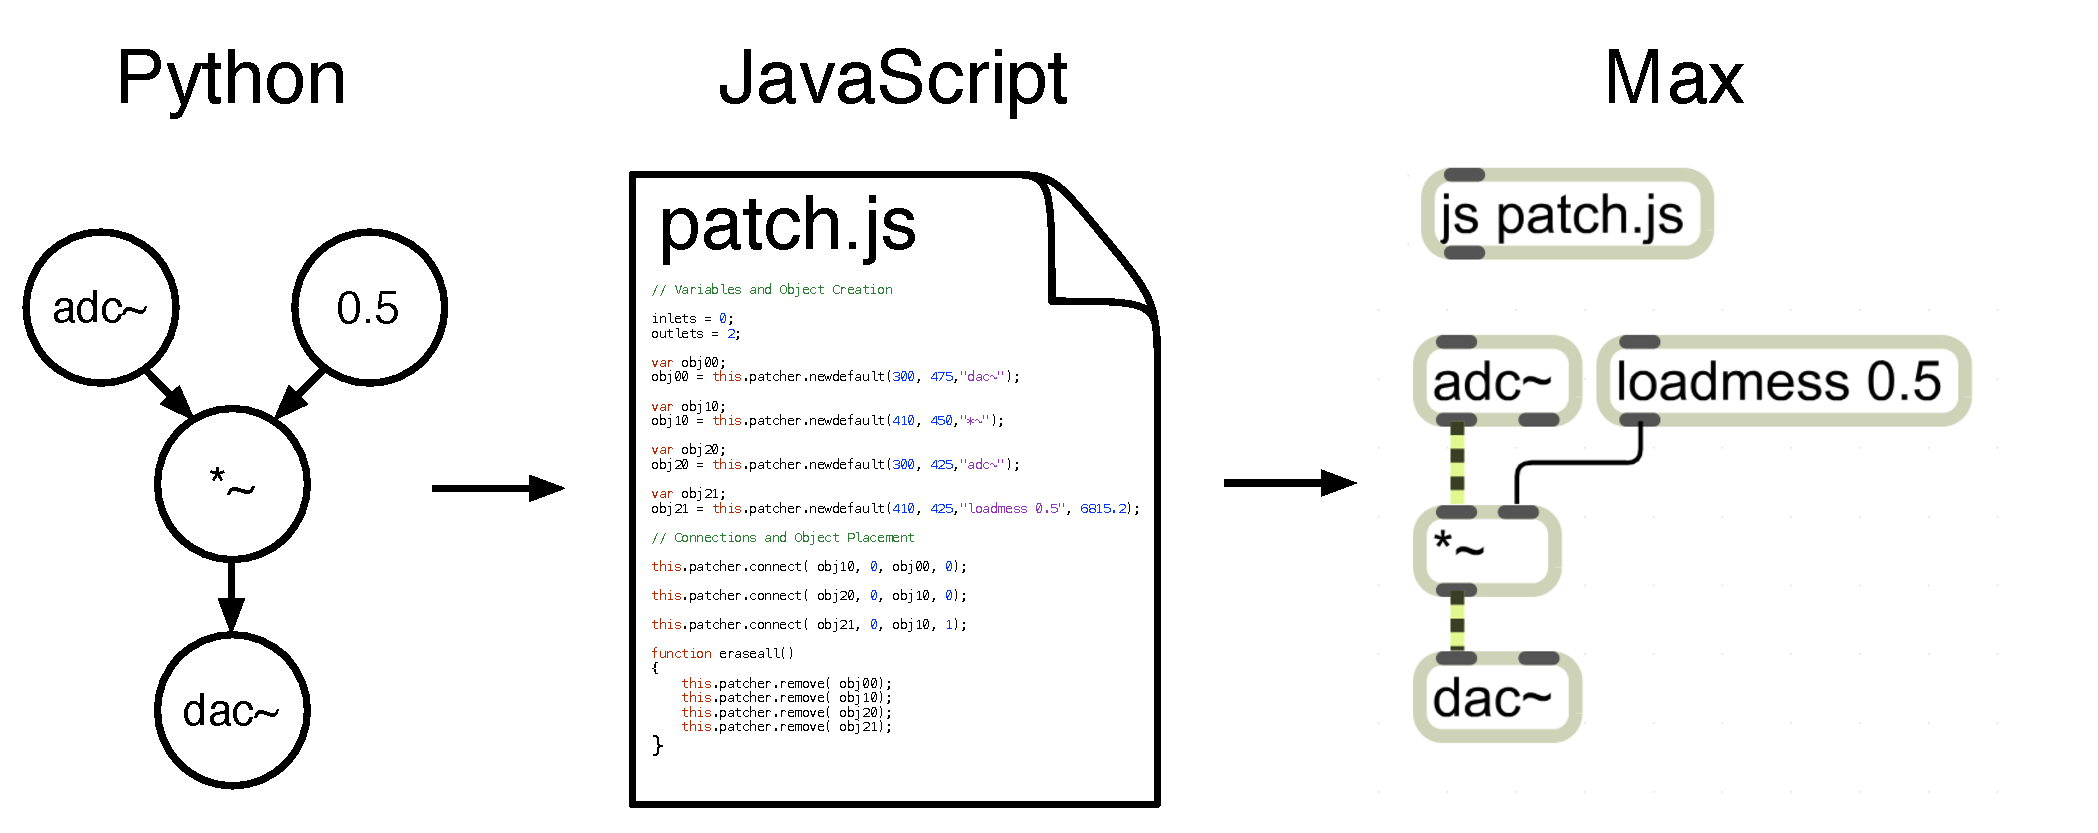
\includegraphics[scale=0.4]{JSTranslation}
\caption[Generating a Max patch given a Python tree]{Translation of a Python \textit{MaxPatch} into an equivalent patch in Max via JavaScript.}
\end{center}
\vspace{6pt}
\end{figure}

The second item is handled by requiring Max to write the generated patch's audio output to a file, which is then read by Python and used for the timbre feature calculation (see Figure 23).
\begin{figure}[h!]
\begin{center}
\vspace{24pt}
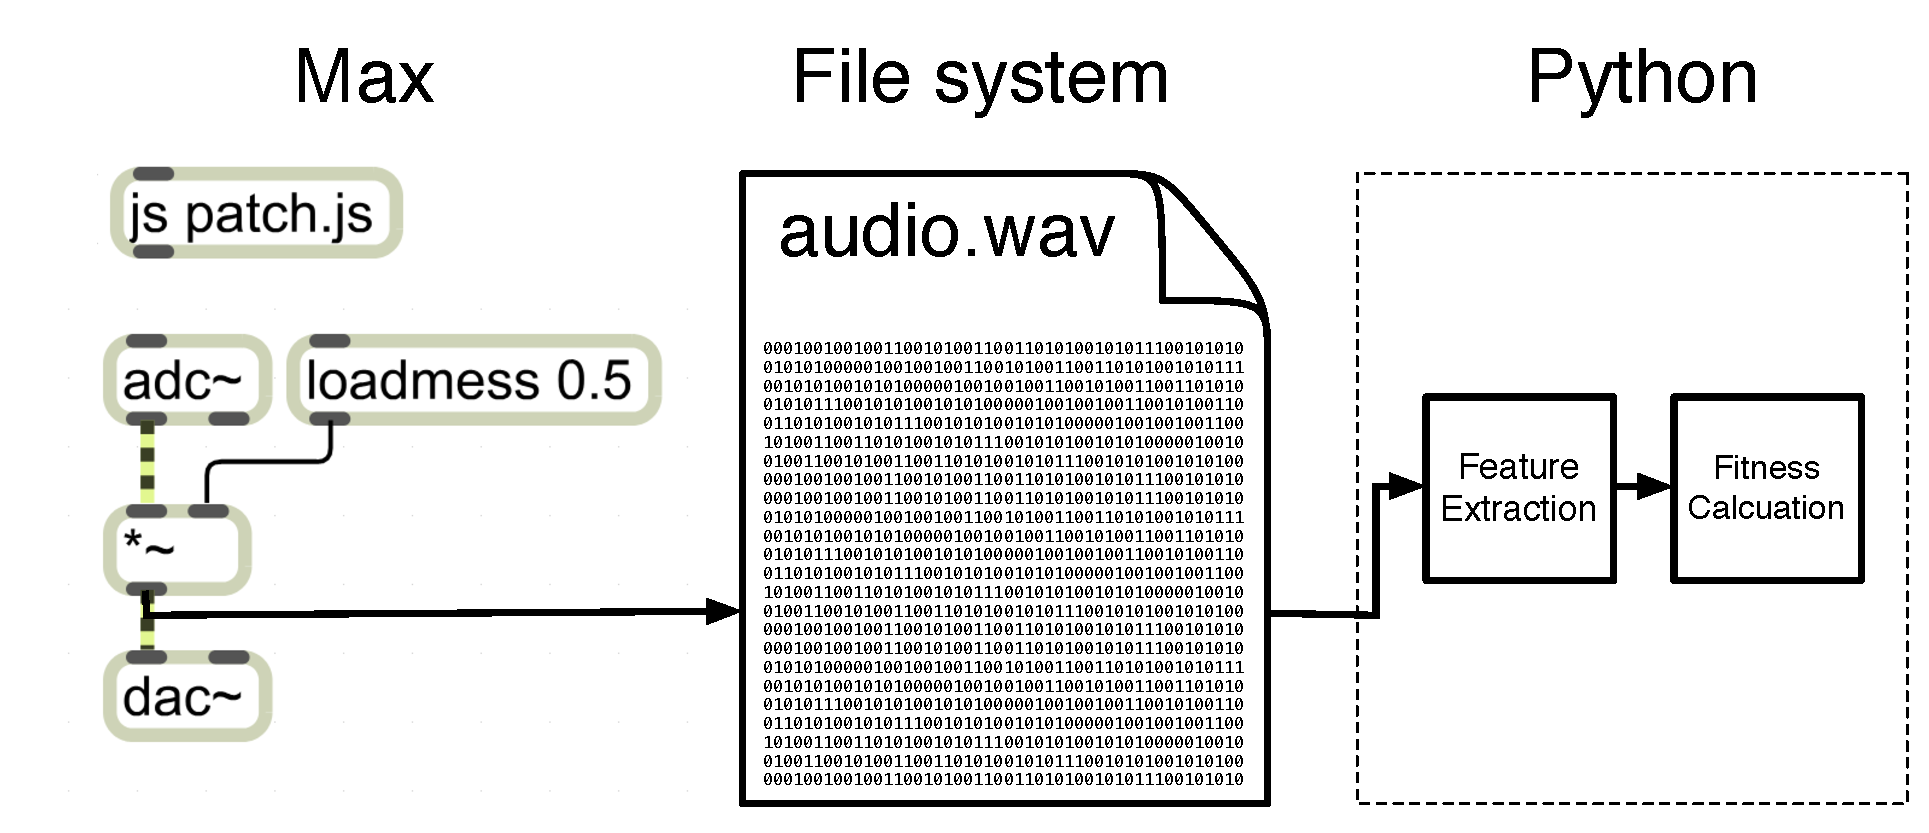
\includegraphics[scale=0.4]{MaxAudioToPython}
\caption[From Max to Python]{Writing audio output from a Max patch to a WAV file that is then read and processed by Python code.}
\end{center}
\vspace{6pt}
\end{figure}

In order to provide Python with an internal representation of a Max patch, we have mirrored all Max constructs using Python classes. For example, we have written MaxPatch, MaxObject, MaxInlet, and MaxConnection classes that represent patches, objects, inlets, and connections in Max. Thus, the initial population creation is done in Python; the resultant patches are translated into JavaScript commands that, via Max's js object, are executed to generate their topologies within Max; audio is generated at the terminals of the patch and sent through its various processing objects; the output at the patch's root is recorded to a file; and Python reads the file and uses its contents to calculate the fitness of the patch. After calculating fitness values for each patch in the population, selection is employed and genetic operators are used to produce the next generation. The process then repeats until a given stopping criterion is met.

\subsection{Framing as a Genetic Programming Problem}
The majority of GP research studies use tree data structures to represent each individual algorithm within a population. We have adopted this representation in evolving Max patches that function as synthesis algorithms. Since Max, in general, allows the creation of graph structures, we have decided to limit the number of possible patch representations by enforcing several rules. 
\begin{enumerate}
\item The root of each tree will be Max's audio output object (the \textit{dac\texttildelow{}}), internal nodes will represent other Max objects that able to receive Max signal input and return Max signal output, and the leaf nodes or terminals will represent either audio generators or input parameters to other nodes (see Figure 24).
\begin{figure}[h!]
\begin{center}
\includegraphics[scale=0.7]{RootTreeFIg}
\caption[A Max patch as a directed tree]{An example Max patch represented as a directed tree with the audio signal flowing from patch's terminals towards its root.}
\end{center}
\vspace{12pt}
\end{figure}

\item By ensuring that at least one terminal is an audio generator, a main signal path can be traced from the input object to the \textit{dac\texttildelow{}}, as seen in Figure 24. Therefore, the patch can be similarly viewed as a black box with audio going in and audio coming out---the fundamental representation of a synthesis algorithm. If more than one audio generator is chosen as a terminal, any could be viewed as that which produces the main signal path, while all others can be regarded as audio-rate input parameters to the system. Thus, the black box representation still holds.
\end{enumerate}

Adhering to the above rules will restrict the search space over all Max patches. Any time such a search space restriction is put in place, one must make sure viable solutions are not left out of the resultant subspace over which the search will occur. Our goal is to search over the space of all synthesis algorithms and not over all Max patches (which occupies a much larger space), so as long as we can be sure that the above restrictions do not leave out any synthesis algorithms, we can proceed without worry.

Any Max patch can be easily be represented by a finite set of \textit{directed acyclic graphs} (DAGs) - where directed edges correspond to Max connections with direction pointing from object outlet to object inlet and vertices/nodes corresponding to Max objects (see Figure 25).
\begin{figure}[h!]
\begin{center}
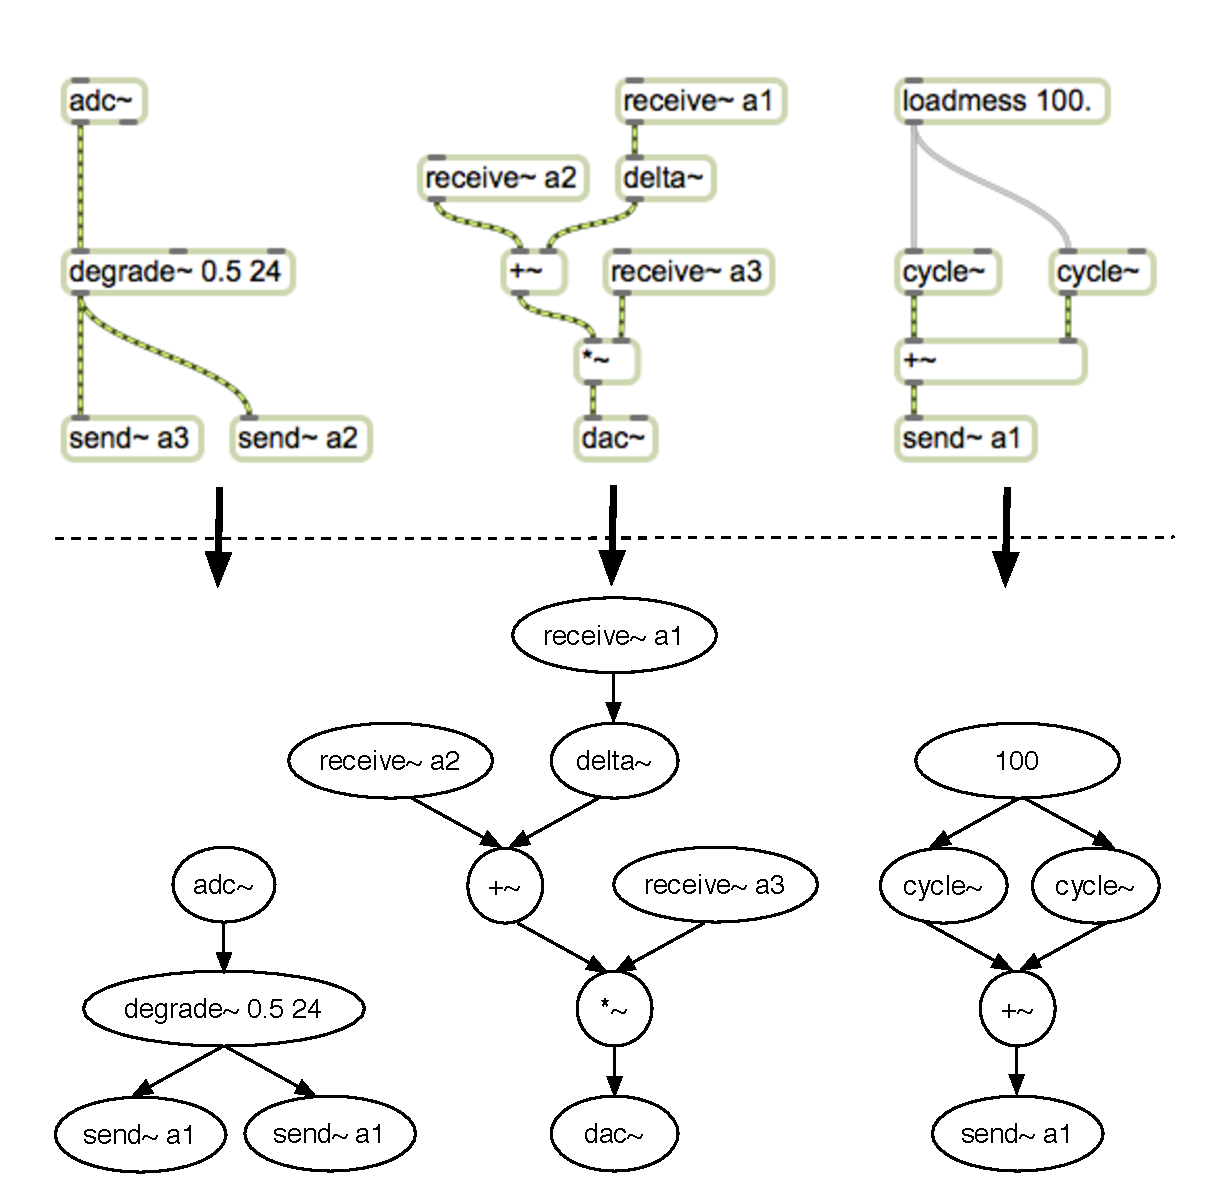
\includegraphics[scale=0.7]{MaxDAGs}
\caption[A Max patch as a set of DAGs]{A Max patch and its corresponding representation as a set of DAGs}
\end{center}
\vspace{12pt}
\end{figure}

Max objects with arguments can often be replaced by their default versions (i.e. those without arguments) and a set of connected \textit{loadmess} objects supplying the same parameterizations of the original object via its inlets (see Figure 26). 
\begin{figure}[h!]
\begin{center}
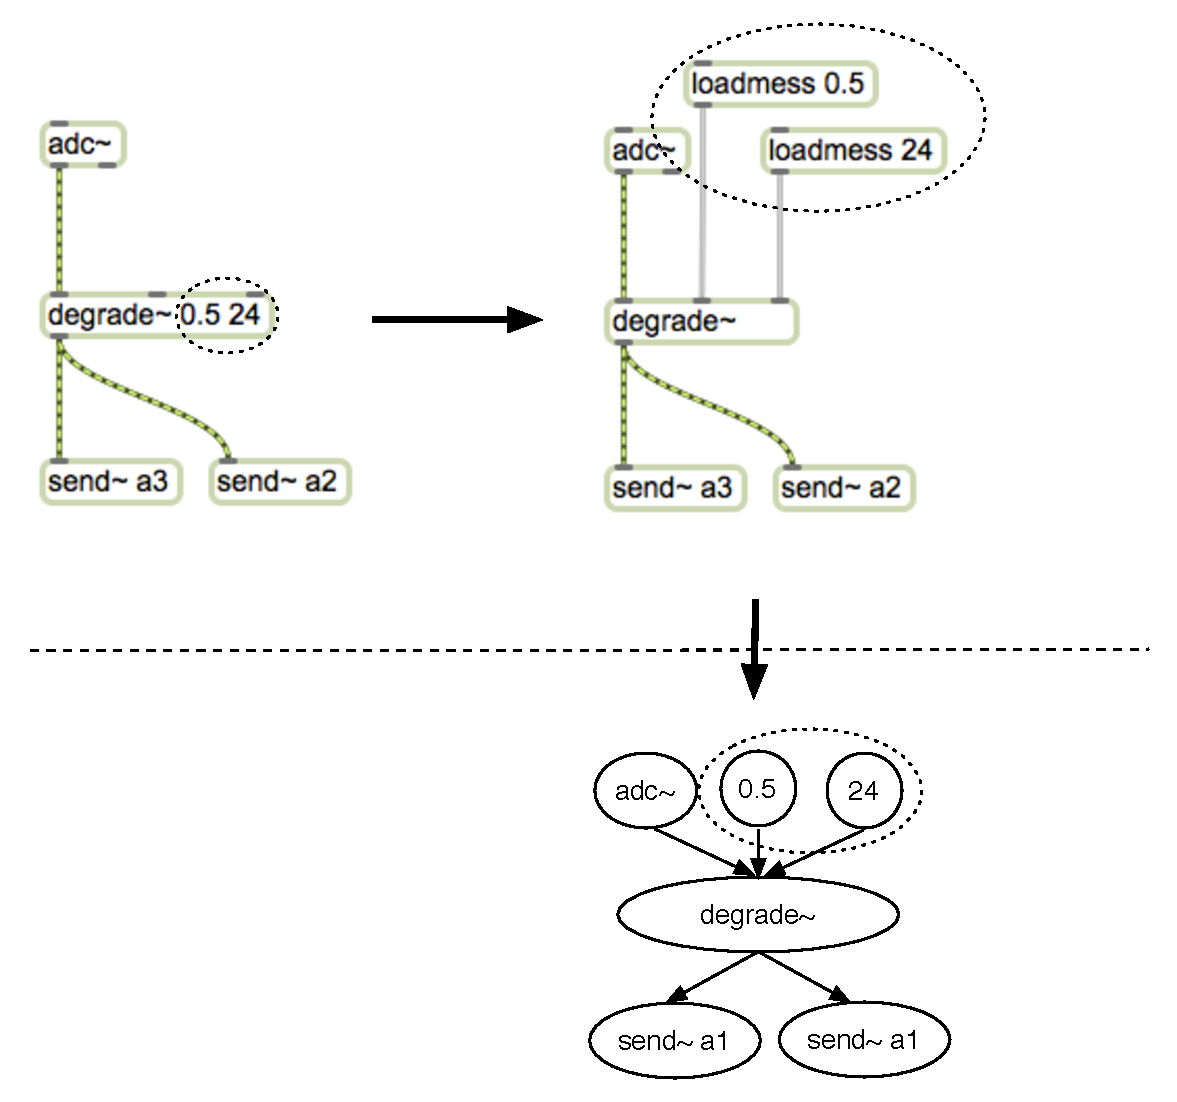
\includegraphics[scale=0.7]{MaxDAGsLoadmess}
\caption[Using \textit{loadmess} objects to provide parameters to Max]{The same \textit{degrade\texttildelow{}} object in two Max patches (one with arguments and one with \textit{loadmess} objects).}
\end{center}
\vspace{6pt}
\end{figure}
These \textit{loadmess} objects act as terminals and help to transform a patch containing objects with arguments and exposed inlets to one with a more direct representation as a set of DAGs.

Max objects come in a number of flavors with regard to what type of data can flow into and out from their connections. The objects that we are primarily interested in are Max's signal processing objects, which output Max's signal data type (i.e. data produced, transformed, and output at the patch's audio sample rate). While Max does provide mechanisms by which to convert its other data types (e.g. matrices of video data, MIDI control rate data) to the signal data type, our research will focus only on the set of objects designed specifically to work with audio data. 

The terminating Max signal processing object for output via an audio device is the \textit{dac\texttildelow{}}. Since any signal processing algorithm must terminate at an output node of this type, the \textit{dac\texttildelow{}} will be required of any patch we wish to search over. If there is only one \textit{dac\texttildelow{}} in the patch, then only the objects in its DAG will contribute to what is sent to the audio output device, unless there is another DAG with a \textit{send\texttildelow{}} (or \textit{send}) object that passes data to an associated \textit{receive\texttildelow{}} (or \textit{receive}) object within the same DAG as the \textit{dac\texttildelow{}}. However, in that case, the send to receive connection can easily be represented by a directed edge. Thus, if we make that substitution in the patch, we are still left with only one DAG containing a \textit{dac\texttildelow{}} (see Figures 27 and 28).
\begin{figure}[h!]
\vspace{15pt}
\begin{center}
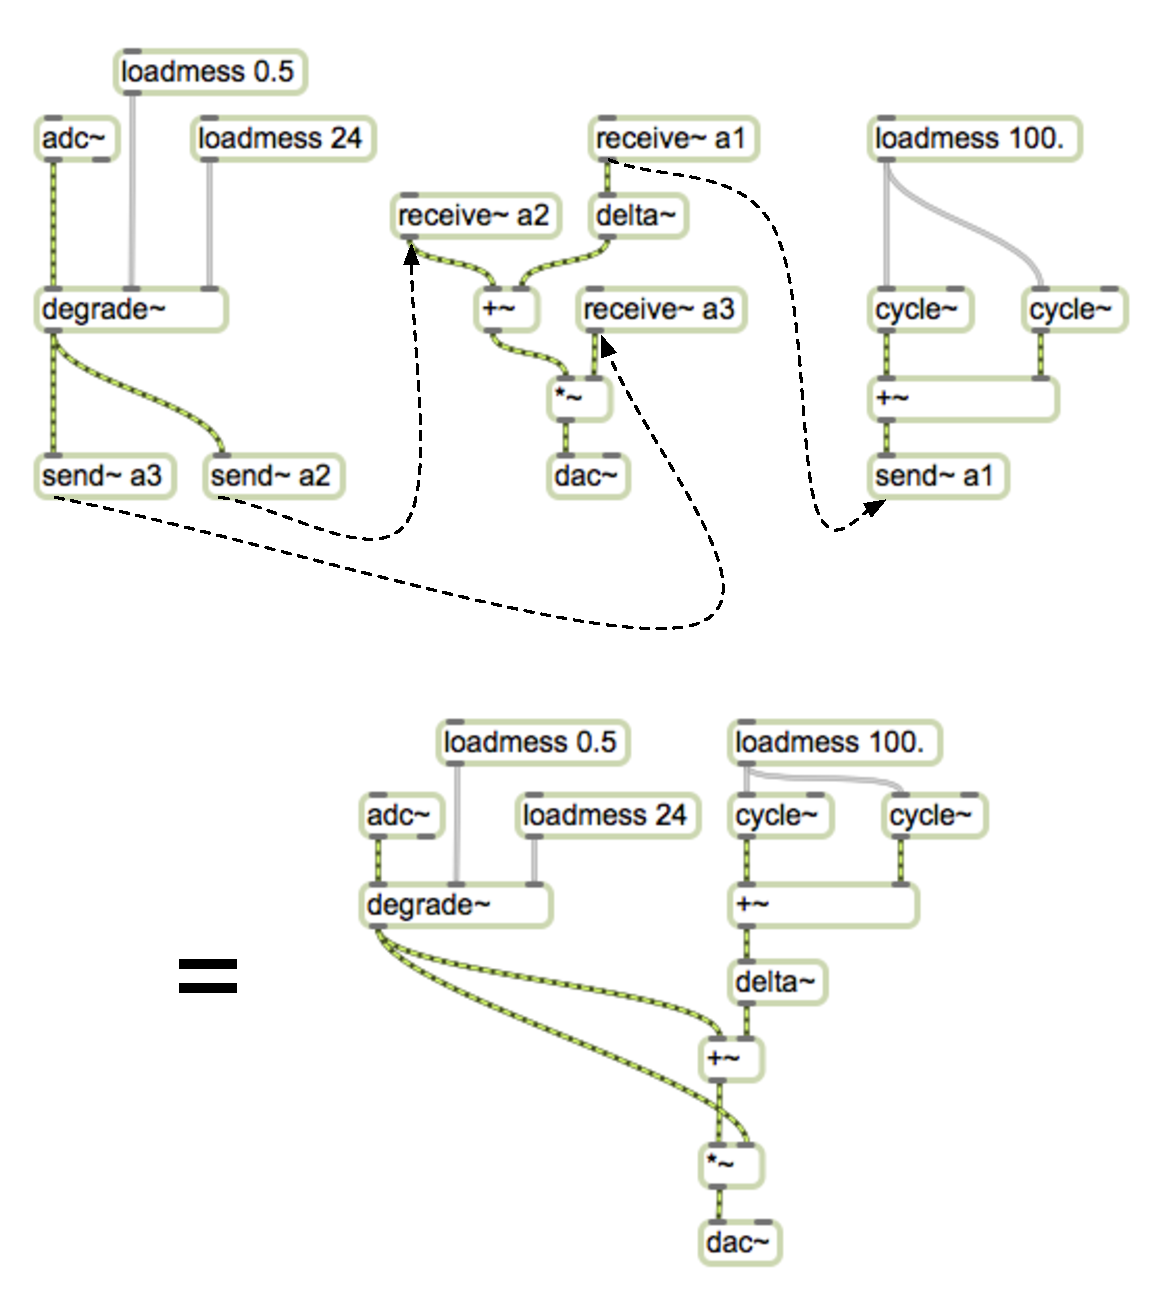
\includegraphics[scale=0.75]{MaxDAGsSendReceive1}
\caption[Removing send\texttildelow{} and receive\texttildelow{} objects]{The original Max patch from Figure 25 replaced by its equivalent patch without send\texttildelow{} or receive\texttildelow{} objects.}
\end{center}
\vspace{15pt}
\end{figure}

\begin{figure}[h!]
\begin{center}
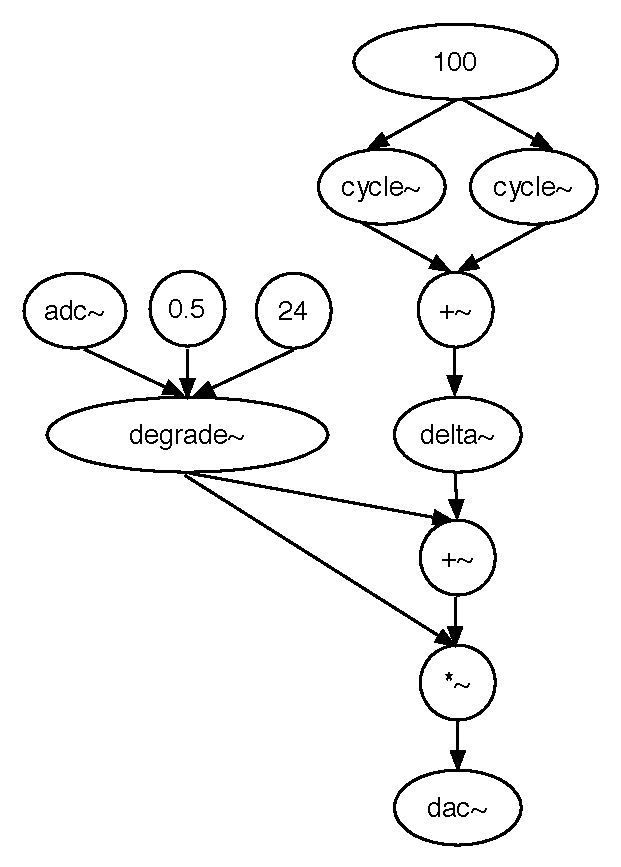
\includegraphics[scale=0.8]{MaxDAGsSendReceive2}
\caption[Reducing a set of DAGs to a single DAG]{The single DAG representation of the reduced patch in Figure 27.}
\end{center}
\vspace{6pt}
\end{figure}
If there are two or more \textit{dac\texttildelow{}} nodes in a DAG or set of DAGs, the signals sent to each of them are simply summed before being sent to the audio output device. Therefore, we can easily model the same DAG with one \textit{dac\texttildelow{}} and one or more \textit{+\texttildelow{}} objects to sum all paths that would normally be summed by Max automatically (see Figure 29). 
\begin{figure}[h!]
\begin{center}
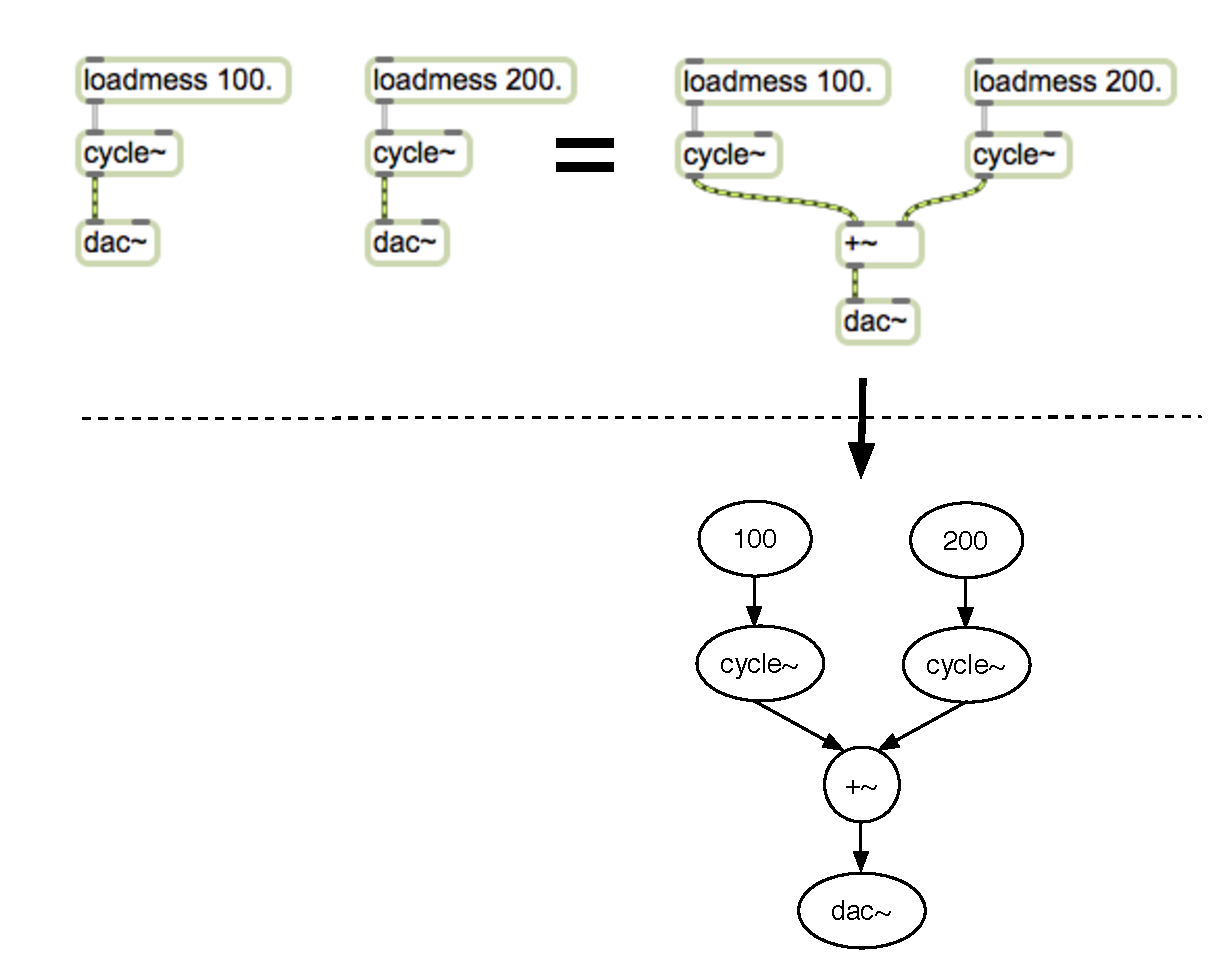
\includegraphics[scale=0.7]{MaxDAGs2DACs}
\caption[A single DAG with two \textit{dac\texttildelow{}} objects]{A single DAG representation of a Max patch with two \textit{dac\texttildelow{}} objects.}
\end{center}
\vspace{9pt}
\end{figure}

The only remaining issue to consider now that we've shown all Max signal processing patches can be reduced to a single DAG with a \textit{dac\texttildelow{}} root is that such topologies can  have two vertices that are connected via multiple paths (see Figure 30), which is not allowed in tree data structures.
\begin{figure}[h!]
\begin{center}
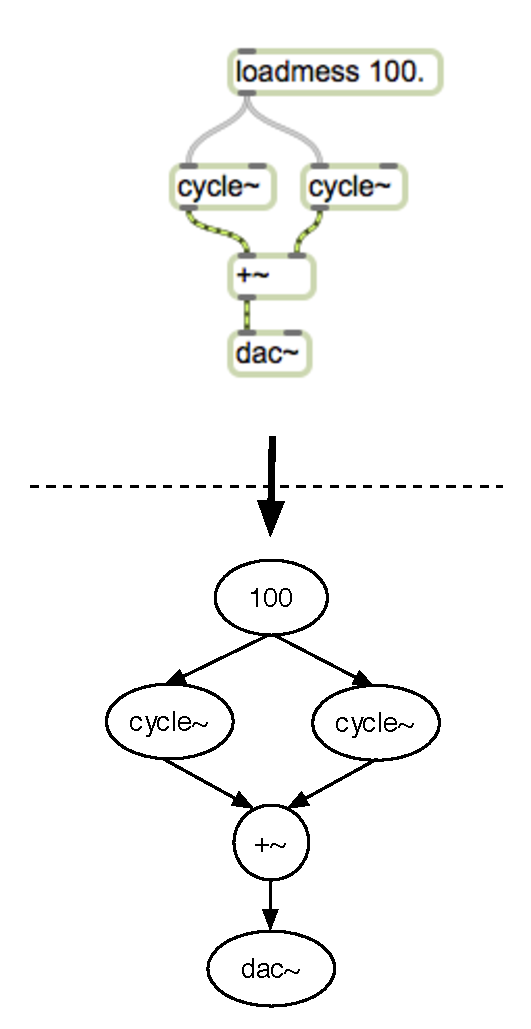
\includegraphics[scale=0.8]{MaxDAGsCrossedPaths}
\caption[A DAG with crossed paths]{A simple Max patch whose DAG representation has crossed paths and therefore is not a tree.}
\end{center}
\vspace{6pt}
\end{figure}
For any two vertices u and v, there is at most one possible path connecting them in a tree. 

However, for every possible DAG representation discussed, there is an equivalent tree representation that can be obtained by splitting each crossed path and duplicating all nodes below it (or \textit{above} it in the visual diagrams presented) (see Figure 31).
\begin{figure}[h!]
\begin{center}
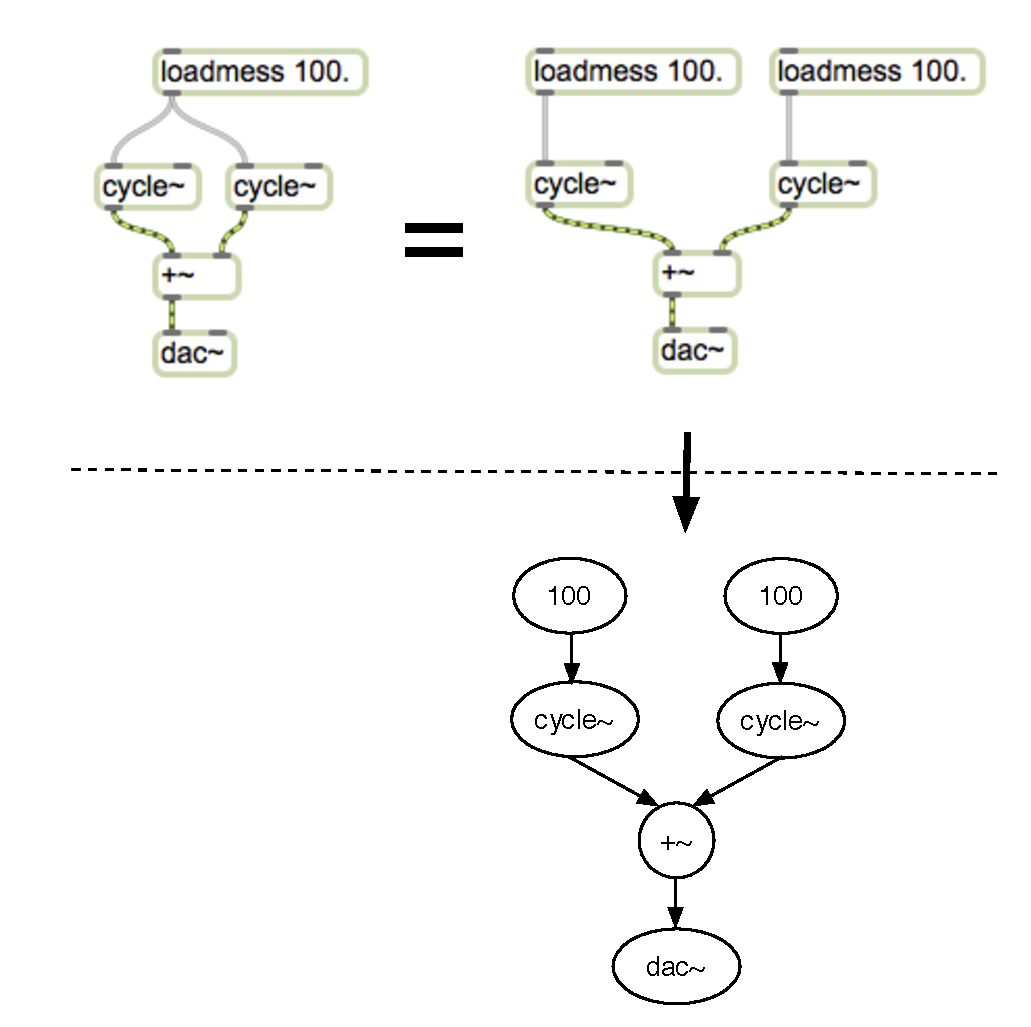
\includegraphics[scale=0.8]{MaxDAGsCrossedPaths2}
\caption[Uncrossing paths to form a tree]{The same Max patch with crossed paths from Figure 30 and its equivalent Max patch with a tree representation.}
\end{center}
\vspace{9pt}
\end{figure}

Therefore, in choosing a standard tree representation to represent all Max synthesis topologies (which is necessary to leverage most work in the GP domain), we are not excluding possible solutions. We next must consider the validity of randomly generated trees given the patch constraints aforementioned.

Starting with a random tree representation of a Max patch can lead to patches that are not syntactically correct. Our trees are only valid representations of Max patches if their edges represent connections that are allowed in the Max environment. In other words, connections to inlets are valid only if the data flowing over those connections are accepted by the inlets. Consequently, syntactic correctness must be enforced while searching over the input-space defined by these trees. Imposing data type constraints during search is a simple way to disregard invalid topologies and make the search much more efficient without excluding possible solutions. This strategy is known as \textit{strongly-typed GP} (STGP). 

Information regarding syntactic correctness in Max is supplied to Python via a text file, which contains a list of Max object names, each followed by their respective inputs' accepted data types and reasonable input ranges, and their output data type (see Figure 32).
\begin{figure}[h!]
\begin{center}
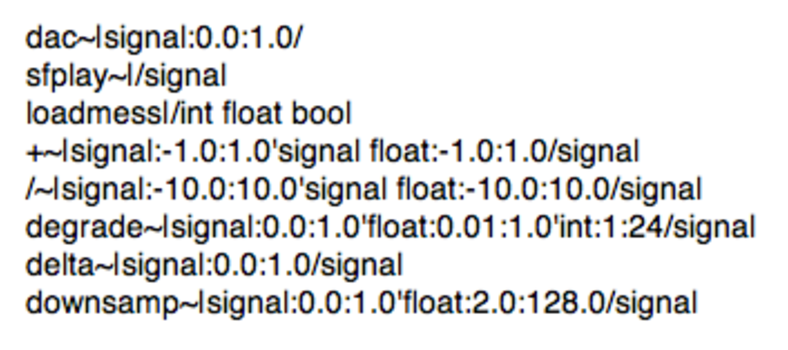
\includegraphics[scale=0.8]{SyntaxInfo}
\caption[Object list file]{Example of the object\_list.txt file that contains syntax information for the various objects used to generate patches with our system.}
\end{center}
\vspace{9pt}
\end{figure}

The format is as follows where the inlet information is simply repeated for multiple inlets and the output type is repeated for multiple outlets (with spaces in between outlet types as shown in Figure 32):
\\
{\textit{objectName\textbar inlet1InputType:minVal:maxVal'.../outletType1 ...}}

\textit{Reasonable ranges} must be chosen carefully as to not be too restrictive, since a particular object may be required to function outside of what is considered its norm in order to contribute to the best solution. Thus, one of the variables we have decided to modify in our experiments is the amount of restriction we apply to each object inlet's range (as discussed in Chapter IV - Experimental Design).

An even more important restriction to consider is the number of unique Max objects available for use in the system (i.e. those for which we provide syntactic information). These objects directly determine the size of the resultant patch subspace over which we search. Therefore, we have also investigated how our system performs by varying the number of objects in an attempt to determine whether a general set exists that is small enough for the search to provide a good solution over a reasonable amount of iterations, but also large enough to provide a solution that produces content that is similar enough to the target to be considered a success. Specifics around the variation of both accepted inlet value ranges and object sets are provided in Chapter IV - Experimental Design.

\vspace{18pt}
\section{Designing the Fitness Function}

Defining the fitness function is how one communicates their objective to the GP system. Without an appropriate definition, the system may discard more-optimal solutions for less-optimal ones from the developer's perspective. This is not a shortcoming of the system itself, but instead of the developer's ability to accurately convey to the system what he is looking for. It is therefore paramount to a system's ability to produce optimal solutions to provide it with a fitness function that objectively measures the usefulness of any given solution in the same way the developer would assign value.

In this research, our objective is to generate Max patches that are able to successfully produce audio that is timbrally similar to some target sound. In order to define a fitness measure for this objective, we need to have a definition of timbral similarity. The definition of an appropriate timbral sequence similarity measure includes both a definition of an objective timbre space, wherein distance between points is semantically meaningful, and a definition of a suitable sequence similarity measure for discrete paths traced through this space. Recent research into timbral similarity already presents a wealth of information that could improve upon the fitness calculations used thus far in research involving the evolution of synthesis algorithms. However, we believe our specific approaches to both timbre feature extraction (i.e. objective timbre space definition) and timbral similarity measurement represent state-of-the-art techniques, which will provide the best chance of evolving synthesis algorithms that accurately model a target sound with time-varying timbre.

Before we can discuss the desired qualities of an objective timbral sequence similarity metric, we first need to have a quantitative measure of timbre. Thus, the first task we face in defining a fitness function is choosing an appropriate timbre feature.

\vspace{12pt}
\subsection{Timbre Feature Extraction}

The design of a semantically valid objective timbre space is essential to the problem of search. If a timbre space has not been chosen such that meaningful timbral similarity measurements can be made, then the fitness landscape will be ill-formed and the search will pursue areas of the input space that are not relevant to the problem.

The MIR community has investigated music similarity on a number of different levels. Some research has been aimed at rhythmic similarity \cite{Paulus:2002ec}, other at harmonic similarity \cite{Haas:2009mw}, and, more recently, structural similarity \cite{Bello:NoRead}. However, timbral similarity has been a main focal point in the community for a number of years. The quest for an appropriate timbral similarity measure has motivated the development of a number of different timbre features (that each define a unique timbre space) for use within similarity models. Initially, this research relied heavily on using the results from the subjective timbre space literature and related studies in speech recognition, but the MIR community's adoption of new advancements in machine learning has resulted in new data-driven methods for timbre feature design.

Early work in timbral similarity was aimed at classifying instruments, which is quite appropriate given that work on subjective timbre spaces could alternatively be seen as generating spaces with good discrimination properties for instruments \cite{Loureiro:2000wq, Park:2004fv, Timoney:2004ff, Zhang:2006jo}. This research takes the viewpoint that timbre is related to its sound-production mechanism and consequently develops models that will assign similar timbre to all sounds generated by the same instrument. Many of the features used in the literature are designed specifically for monophonic instrument sounds and do not apply to polyphonic mixtures or more complex timbral evolution \cite[p. 6]{Ciglar:2009uf}. For example, these include features that measure the temporal progression of an instrument's harmonic partials, features related specifically to the attack, sustain, and release portions of a note, as well as strength relations between odd/even partials \cite[p. 182]{Timoney:2004ff}. In order to develop a more general timbre feature representation, applicable to both monophonic and polyphonic sounds, the community focused on a more complex problem: genre recognition.

Genre recognition systems are primarily interested with timbre on a global time scale (i.e. over an entire song). It is because of this large body of research that Johnson and Gounaropoulos make a distinction between local and global timbre \cite{Johnson:2006pi}. However, even though genre recognition systems are not necessarily interested in local timbral evolution (as we are), genre recognition research requires a representation of timbre for complex polyphonic signals, and thus a lot can be learned from such work.

Aucouturier and Pachet were two of the first researchers to investigate a system for genre classification \cite{Aucouturier:2002gf}. The underlying assumption in genre recognition is that each genre has unique timbral properties on the global scale and therefore by measuring these properties given an unlabeled song, one is able to automatically assign it a genre. Aucouturier and Pachet borrow a feature set from the speech community known as Mel-frequency cepstral coefficients (MFCCs) that have now become ubiquitous as timbre features \cite[p. 1]{Aucouturier:2002gf}. In speech processing research, ``MFCCs were developed to model the spectral envelope while suppressing the fundamental frequency'' \cite[p. 1]{Jensen:2006dw}. Thus, they are often considered to be a compact representation of the spectral envelope (a typical feature included in the additive definition of timbre) divorced from pitch (a property from the subtractive definition of timbre). Aucouturier and Pachet model the probability density of all of the MFCCs from a genre using a Gaussian mixture model (GMM), which is simply a multimodal (and often multivariate) distribution composed of Gaussian components (see Figure 33). 
\begin{figure}[h!]
\vspace{24pt}
\begin{center}
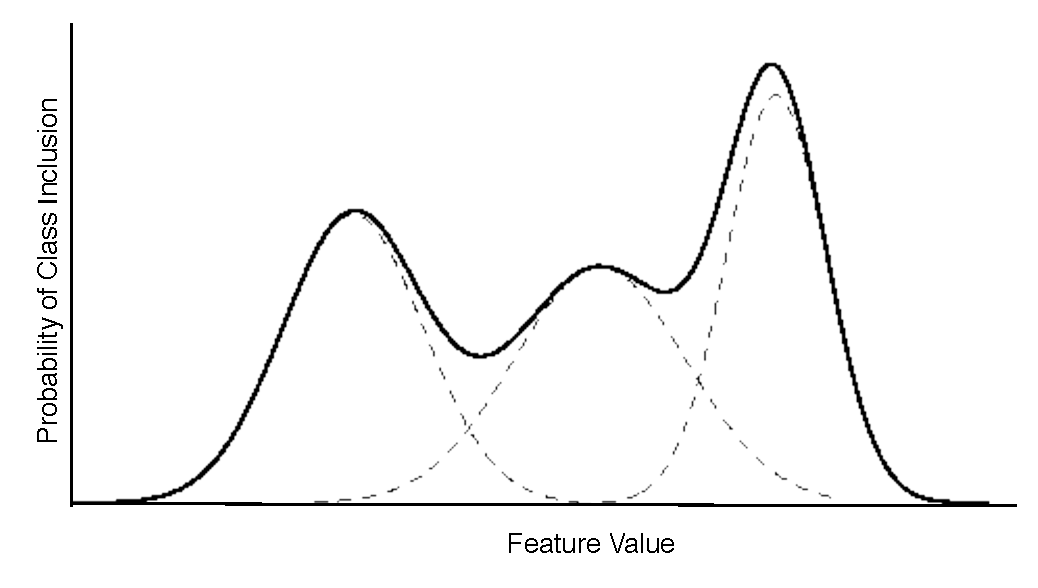
\includegraphics[scale=0.70]{GMM}
\caption[Gaussian mixture models]{An example of a univariate Gaussian Mixture Model (GMM) taken from (Schwardt, 2005).}
\end{center}
\vspace{6pt}
\end{figure}
In order to determine the genre of a set of test samples, MFCCs are extracted and their likelihood under each genre model is calculated. The most likely genre is assigned to the set of test samples \cite[p. 2]{Aucouturier:2002gf}.

Following the work of Aucouturier and Pachet, Pampalk also modeled the timbral content of music with GMMs of MFCCs in his dissertation on sound similarity \cite{Pampalk:2006pr}. However, instead of classifying songs by genre, Pampalk was primarily interested in calculating pairwise similarity between songs. He separately modeled each song with a GMM and calculated the similarity between GMMs using two common distance metrics for probability distributions: Kullback-Leibler (KL) divergence and earth mover's distance (EMD) \cite[p. 26]{Pampalk:2006pr}. Roughly speaking, KL Divergence (also known as relative entropy in Information Theory literature) is a measure of how well one distribution approximates another (and is therefore not symmetric) while the EMD is a measure of \textit{how much} one would have to change the shape of one distribution in order for it to look like the other. Determining whether such models are appropriate for pairwise similarity is a difficult task. In order to properly measure the accuracy of a given model, a sound similarity ground truth must be designated.

As noted by Seyerlehner and Widmer, ``ideally, a content-based audio similarity metric should approximate the ill-defined \textit{sounds-like} related for songs'' \cite[p. 1]{Seyerlehner:2008tw}. However, Logan, Ellis, and Berenzweig point out that similarity ratings can vary ``not only across users, but across time, according to mood and according to context'' \cite[p. 1]{Logan:2003cr}. This is verified by Pampalk et al. \cite[p. 6]{Pampalk:2008xz}. By testing enough users, one may be able to form a meaningful consensus, but user-testing is expensive (both in time and money) and alternate ground truth data is often desired. Consequently, some other labeling is usually accepted (e.g. genre), whether it is provided by experts or by clustering user-provided tags \cite[p. 2]{Logan:2003cr}. The extent to which this data approximates \textit{sounds-like} is unclear. An even more important question, however, is whether \textit{sounds-like} on the global timescale is truly a measure of similarity between two songs. Many other factors could \begin{singlespace}
\noindent play a role (e.g. lyrical content, popularity). In Jensen's dissertation, he writes that:
%\linespread{1}
\selectfont
\begin{quote} The inherent problem, that genres are a cultural as much as a musical phenomenon, persists...in our opinion, genre classification as a research topic in signal processing should be abandoned in favor of specialized tests that directly evaluate the improvements of proposed algorithms. The short time features that only capture timbral similarity, or methods using source separation, could e.g. be tested in a polyphonic identification setup that much better shows the capability of the algorithms \cite[p. 11]{Jensen:2009ta}.
\end{quote}
%\linespread{1.7}
\selectfont
\end{singlespace}
Aucouturier and Pachet do note in their 2003 paper that in studying genre recognition, ``the problem of the actual perception of timbre is not addressed by current methods'' \cite[p. 16]{Aucouturier:2003gs}. However, this facet of MIR continued to be synonymous with timbral similarity for a number of years and was used to measure the accuracy of systems like Pampalk's \cite{Pampalk:2006pr}. The fact that genre classification results did not see any marked improvements over that time was actually a good thing for timbre research, because it stimulated a wide variety of approaches towards finding better timbre features and incorporating them into better similarity models.

For example, Meng, Ahrendt, and Larsen attempted to improve genre classification results by integrating short-time timbre features, on the order of $30$ms, into medium (on the order of $740$ms) and long-term (on the order of $9.62$s) timbre features in order to better model the temporal evolution of timbre on longer time scales \cite[p. 498]{Meng:2005fx}. The authors suggest calculating simple statistics, using dynamic PCA (where features are stacked over the desired time horizon and PCA is used to reduce the dimensionality of the resultant feature vector), and modeling the time-varying properties of a sequence of MFCCs by calculating the power spectrum of each (p. 498). They found best results using these latter features, which they called filter-bank coefficients (FCs). These features are able to capture MFCC modulations over a number of modulation rates (with a resolution determined by the length of the time horizon). 

Heise et al. use similar features to Meng et al.'s FCs \cite{Heise:2009sp}. Instead of calculating the power spectrum of each MFCC over a specified time window, they compute a discrete cosine transform (DCT), which decorrelates and compresses the MFCCs spectral data into the first few bins while retaining the characteristics of its shape. The result is a MFCC spectral matrix where each row represents a different MFCC. The authors reduce the dimensionality of this feature matrix by either throwing away the high MFCCs (retaining good MFCC spectral resolution, but smoothing out the signal's spectral envelope), or by throwing out the last columns (retaining good signal-spectral-envelope resolution, but smoothing out the MFCC spectral resolution) (2009, p. 3).

Pampalk, Flexer, and Widmer develop fluctuation pattern (FP) features that are derived from a perceptually transformed spectrogram. Again, like Meng et al. and Heise et al., these authors incorporate the temporal evolution of the features by taking the FFT over each band in their perceptual spectrogram \cite[p. 4]{Pampalk:2005ix}. They find that incorporating these features do not improve genre classification performance, but again, this does not necessarily mean that they are not modeling the timbre more accurately \cite[p. 8]{Pampalk:2005ix}.

Incorporating the temporal evolution of timbral features over some time horizon using the FFT of each feature over that horizon is an interesting idea that requires more research outside of the domain of genre recognition so that it may be fairly evaluated.

A number of other features have been used alongside MFCCs (on the same time scale) in hopes that additional timbre information will be contained in some or all of them. Most often, due to the curse of dimensionality, feature selection methods are used to find those features that boost performance the most, while filtering out those that provide marginal contribution. 

Allamanche, Herre, Hellmuth, Kastner and Ertel start with a set of features including normalized loudness, delta log-loudness, spectral flatness measure, spectral crest factor, real cepstral coefficients, spectral tilt, spectral sharpness, and zero crossing rate along with MFCCs \cite{Allamanche:2002yo}. For feature selection, they perform a greedy search by first finding the single feature that provides best classification, then adding to it the feature that helps it perform best, etc.

McDermott et al. investigate 40 different features commonly used in MIR research and eliminate features based on their redundancy in the presence of others \cite[p. 1]{McDermott:2005xq}. The authors split these features into six groups, based on the type of feature---time domain, Fourier-transform domain, partial domain, trajectory, periodic, or statistical---and find that features within the same group tend to be redundant in the presence of others in that group, an un-alarming result \cite[p. 6]{McDermott:2005xq}.

Seyerlehner et al. take a subtractive approach to feature \textit{selection} by searching for feature vectors that are not perceptually relevant (e.g. silence) and filtering them out \cite{Seyerlehner:2009hs}. They note that in modeling a feature vector sequence containing some silent frames using a GMM, the distribution will contain a peak at the silent location in space. Thus, if another feature vector sequence's likelihood is computed and it also has silent frames, then a non-negligible likelihood will result no matter how different the non-silent frames are from one another between the two sequences. The authors find that these low energy frames thus contribute greatly to the measure of similarity, which is undesirable \cite[p. 3]{Seyerlehner:2009hs}.

Another option in contrast with feature selection is intelligent feature combination, proposed by Fu et al. for the task of timbre feature design \cite{Fu:2009mz}. As opposed to selecting a subset of features that improve classification over the entire feature set, feature combination attempts to combine all features in a way that improves performance over any single feature vector.

Kobayashi uses evolutionary algorithms to breed linear combinations of features that provide the best classification performance \cite{Kobayashi:2009la}. His system is based around instrument recognition, but the principle would be valid for any type of classification. As opposed to Pachet and Roy's work \cite{Pachet:2007if} on using GP to breed a single discriminatory feature, Kobayashi starts with a general feature set, able to extract information from scalars, vectors, and/or matrices, and evolves the best linear combination of discriminatory features.

Evolving features or proper combinations of features is a natural direction for feature selection. Instead of relying on hand-crafted feature sets and information-theoretic assumptions about what makes a feature \textit{useful}, these methods evolve functions that well-suited for their problem-domain. A downside to such methods, however, is that one must evolve a new feature or set of features for each problem.

Determining the most appropriate objective timbre representation is still an unsolved problem. One may find, for example, that the best timbre representation comes from its subtractive definition (by removing pitch and loudness) rather than its additive definition, which is equally flawed. While MFCCs are ubiquitous as timbre features, BOF approaches (requiring feature selection or combination) and early fusion techniques have potential to improve upon this representation. However, while these methods expand the space of feature possibilities by looking not only at hand-crafted features, but also concatenations and linear combinations of them, there is a strong reliance on the assumption that all important timbral information is contained in this hand-crafted feature space. Additionally, these methods presume that a combination of hand-crafted features exists that not only contains all timbral information, but also that contains little information about any other musical dimensions (i.e. the feature combination has little noise). A more direct approach to learning low-noise timbral features is to not limit the feature space to only contain linear combinations of hand-crafted features, but instead to allow more fundamental building blocks from which to generate/learn timbral features.

Humphrey, Glennon, and Bello posit that is it  ``advantageous to automatically learn features from some minimally processed input representation'' rather than hand-craft a feature set that would produce a semantically meaningful timbre space \cite{Humphrey:2000th}. In short, learning features allows one to explicitly specify how they want a feature-space organized (in their case, well-clustered instrument samples) and leverage machine learning algorithms to find an optimal space for that criteria, whereas designing features based either on perceptual models or what one believes to be the important information content related to a task is just a guessing game with no proven iterative search strategy, likely excluding optimal solutions simply because they are non-intuitive or obfuscated from the researcher in some way.

Humphrey et al.'s \cite{Humphrey:2000th} work directly learns timbre features using machine learning architectures known as  \textit{convolutional neural networks} (CNNs). Their approach learns a nonlinear projection from basic high-dimensional spectral representations of audio to a low-dimensional space where distances are semantically meaningful in the sense that two points that are close together will be considered timbrally similar and two points that are far apart, dissimilar. Their work focuses on the instrument recognition task and uses an iterative learning process to ensure that two sounds that are transformed by the same projection that come from the same instrument resolve down to points that are close in timbre space. The nonlinear projection imposed by the resultant CNN can be viewed as feature extraction, where projected points reside in a feature space that is representative of timbre.

The underlying assumption they make is that sounds from the same instrument should cluster well in a semantically meaningful timbre space (i.e. the ratio of variance between classes/instruments should be much greater than the variance within classes/instruments). In other words, all sounds produced by the same instrument have similar timbre, regardless of playing technique. However, as noted by Pampalk, Herrera, and Goto in referring to timbral studies that use instrument classification as a means of evaluation, ``instrument class data only allows comparison on the instrument level. Judgements within an instrument class cannot be evaluated directly'' \cite[p. 9]{Pampalk:2008xz}. 

We can infer that any timbre space with well-separable instrument clusters will be organized over instrument sounds at a high-level similarly to the optimal space. However, there may be several spaces sharing similar high-level organization with the optimal space that differ wildly in their low-level (i.e. within instrument group) organization. There also may be numerous spaces that are organized well at a high-level regarding instrument class, but that do not generalize well to non-instrumental sounds. Therefore, a more rigorous treatment should be carried out that additionally measures both the low-level appropriateness of a timbre space that has proven to organize instrument classes well and its capability of organizing non-instrumental sounds in a semantically meaningful way, but we leave this treatment to future work as it could fill an entire dissertation on its own.

For the scope of this study, we seek to find an objective timbre feature space that organizes instrument samples well enough to achieve state-of-the-art instrument recognition results when paired with a simple classifier. This was similarly the goal of Humphrey et al.

The relationship between classification performance and timbre space suitability provides an indirect means of testing a given timbre space. By using an unsophisticated classifier, we fully expose the organization of the space and how well instruments are clustered within it. A sophisticated classifier could overcome minor faults in this organization and so we look to the simplest classifier that would still be viable in a well-organized space.

One of the simplest classification algorithms is nearest neighbor (NN) classification. In this case, NN would consist of mapping a large database of instrument sound samples into an objective timbre space and measuring how well they cluster over instrument class by randomly choosing samples in the space, searching for their nearest neighbor in that space, and recording whether that neighbor was produced by the same instrument or not. One would then be able to compare multiple objective spaces by using the \textit{classification} accuracy found during the experiment. NN classification is often extended to reduce noise by selecting the k-nearest neighbors (kNN) and labeling the test sample using the class with highest cardinality among them (see Figure 34).
\begin{figure}[h!]
\begin{center}
\vspace{12pt}
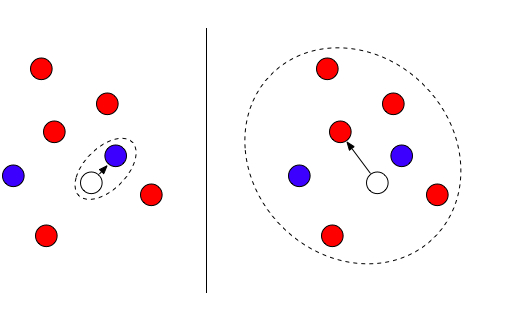
\includegraphics[scale=0.5]{NearestNeighbor}
\caption[Nearest-neighbor vs. k-nearest-neighbor classifier]{Nearest-neighbor vs. k-nearest neighbor classifier - the test sample (white) is set to the blue class in nearest-neighbor classification and to the red in k-nearest neighbor classification where k = 7}
\end{center}
\vspace{6pt}
\end{figure}
Taking the above into consideration, Humphrey et al. decided to measure the appropriateness of a given objective timbre space by running an instrument classification experiment on it using a kNN classifier.

The technique they developed to learn an appropriate timbre space where different instruments are well-clustered is titled \textit{non-linear semantic embedding (NLSE)}. In the 
\begin{singlespace} 
\noindent paper introducing NLSE they note:
\begin{quote}
NLSE addresses the limitations of current statistical dimensionality reduction techniques, such as MDS, PCA or LLE [because] unlike these methods, NLSE explicitly encodes semantic information in the transformation, makes minimal assumptions about salient acoustic features, generalizes well to unseen [instrument] data and produces an output space where [Euclidean] distance is meaningful \cite[p. 1]{Humphrey:2000th}.
\end{quote}
\end{singlespace}
NLSE utilizes a pairwise CNN model based upon Hadsell, Chopra, and LeCun's work on \textit{Dimensionality Reduction by Learning an Invariant Mapping} (DrLIM) \cite{hadsell2006dimensionality}. CNNs are a special kind of \textit{neural net} that combines convolutional layers (where inputs are convolved with 2D filters, whose values are trainable) that are typically separated by a downsampling operation and a non-linear squashing function (see Figure 35). 
\begin{figure}[h!]
\begin{center}
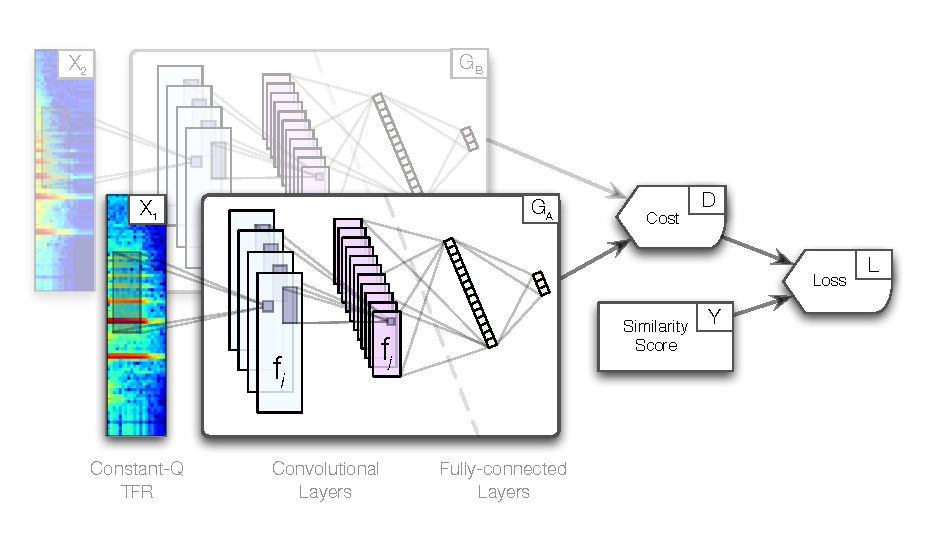
\includegraphics[scale=0.95]{PairwiseCNN}
\caption[Pairwise CNN architecture]{Pairwise CNN used to learn an objective timbre space from various pairs of within class and between class instrument samples.}
\end{center}
\vspace{6pt}
\end{figure}
After a succession of these convolution layers, CNNs most often use standard fully-connected neural net layers to reduce the dimensionality of the data before output. The benefits of CNNs are found in the translation invariance their convolutional layers provide, and scale invariance the downsampling operation provides. When the input to a CNN is a time-frequency representation as is the case in our problem domain, these invariances correspond to small invariances in temporal shifts and scalings in our data (important because we should not suppose that all samples will be precisely temporally aligned or that their timbral information will evolve precisely in the same manner) and small invariances over our frequency scale. The latter invariance is important to extracting timbre from a signal, because it is generally believed that timbre does not correlate with pitch variation. It is possible to utilize the inherent frequency scale invariance that CNNs provide to better eliminate any dependencies in our output space on pitch by using a time-frequency representation that is linear in pitch. For this reason, Humphrey et al. chose a constant-Q time-frequency representation as is shown in Figure 35, where bins are spaced equally in pitch space rather than in frequency space.

Hadsell, Chopra, and LeCun's work on DrLIM utilizes a pairwise CNN architecture (i.e. two CNNs with the same exact structure) with tied weights to learn a low-dimensional invariant mapping from a high-dimensional input space \cite{hadsell2006dimensionality}. The training phase consists of sending both positive (i.e. samples from the same instrument) and negative (i.e. samples from two different instruments) examples through the CNNs and adjusting the tied weights such that semantically similar items are placed near each other in the output space and semantically dissimilar items are placed far away from each other in the output space. This is accomplished using what is known as a \textit{contrastive loss function}. A contrastive loss function is one that returns small values for positive examples that are close to one another in the output space and large values for positive examples that are far away from one another in the output space. Conversely, small values are returned for negative examples that are far away from each other in the output space and large values for negative examples that are close to each other in the output space. Specifically, the loss function Humphrey et al. chose that meets this criteria follows:
\begin{equation}
L(X_1, X_2, Y|W)=Y*L_{sim}(D)+(1-Y)*L_{Diff}
\end{equation}
The inputs $X_1$ and $X_2$ to $L$ represent constant-Q time-frequency patches, $Y$ is the semantic similarity score between inputs taking a value $[0,1]$ and $W$ represents the parameters of the CNN architecture. $L_{Sim}(D)$ and $L_{Diff}(D)$ are the similarity loss and difference loss, respectively and $D$ is some cost function associated with the outputs of the architecture, often labeled $Z_1$ and $Z_2$. In this work, the cost function is simply the Euclidean distance between the points $Z_1$ and $Z_2$.

The only contributor to the contrastive loss, L, is the similarity loss when $Y=1$ (i.e. the items are maximally similar) the difference loss when $Y=0$ (i.e. the items are maximally dissimilar). Since the loss should increase for similar items that are far apart, Humphrey et al. chose the following similarity loss (known as the square loss):
\begin{equation}
L_{Sim}=\frac{1}{2}Y*D^2
\end{equation}
As the distance between points increases, so does the loss. 

Conversely, the difference loss (which contributes most when items are maximally dissimilar) should increase as the distance between $Z_1$ and $Z_2$ decreases. Therefore, Humphrey et al. chose the following difference loss (known as the \textit{log-loss}):
\begin{equation}
L_{Diff}=\frac{1}{2*Q^2}*log\Big(1.0+e^{Q*(m-D)}\Big)^2
\end{equation}
The parameters $m$ and $Q$ are used to define the loss function's \textit{margin} and \textit{knee} respectively, but the details of this are not important. The key thing to note is that as $D$ decreases, $e^{Q*(m-D)}$ increases, which in turn increases $L_{Diff}$ as desired.

By using standard back propagation methods, one is able to update all the trainable parameters in the CNN architecture so that, over $N$ iterations, the parameters converge to a stable state (and hopefully a global optimum). Once convergence occurs, the resulting pairwise architecture represents two copies of a CNN that has learned a low-dimensional invariant mapping from the high-dimensional input space of your original data (e.g. patches of constant-Q spectra) into a semantically meaningful low-dimensional space. In our problem domain, this means a timbre space where samples from the same instrument class are well clustered and instrument clusters are well-separated.

Humphrey et al. show that the objective timbre space generated (and the corresponding features that define the space) using the above method outperforms the leading alternative timbre-feature in the literature (MFCCs) - after the typical PCA (Principal Component Analysis) and LLE (Locally Linear Embedding) dimensionality reduction techniques have been applied - on instrument classification tasks involving up to 12 different instruments (see Figure 36 for kNN accuracy up to 9 instruments) \cite{Humphrey:2000th}.
\begin{figure}[h!]
\begin{center}
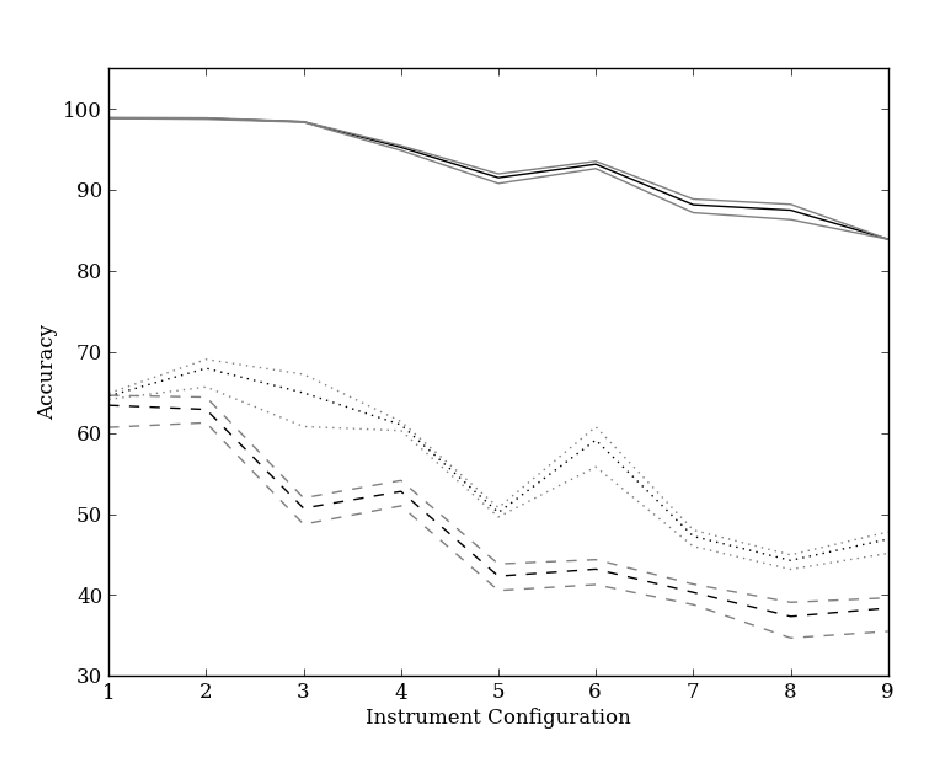
\includegraphics[scale=0.85]{CNN_kNN}
\caption[kNN accuracy for NLSE, PCA, and LLE]{The mean, min, and max kNN accuracy for experiments varying k using NLSE (solid lines), PCA (dotted lines), and LLE (dashed lines).}
\end{center}
\vspace{6pt}
\end{figure}
Specifically, NLSE remains at a classification accuracy above 90\% until 7 instruments are introduced, while PCA and LLE are both between 30\%-40\% lower than NLSE for all cases.

For some insight on how the objective timbre output spaces are organized in the NLSE, PCA of MFCC, and LLE of MFCC cases, see Figure 37 showing the distribution of instrument samples for 5 different instruments.
\begin{figure}[h!]
\begin{center}
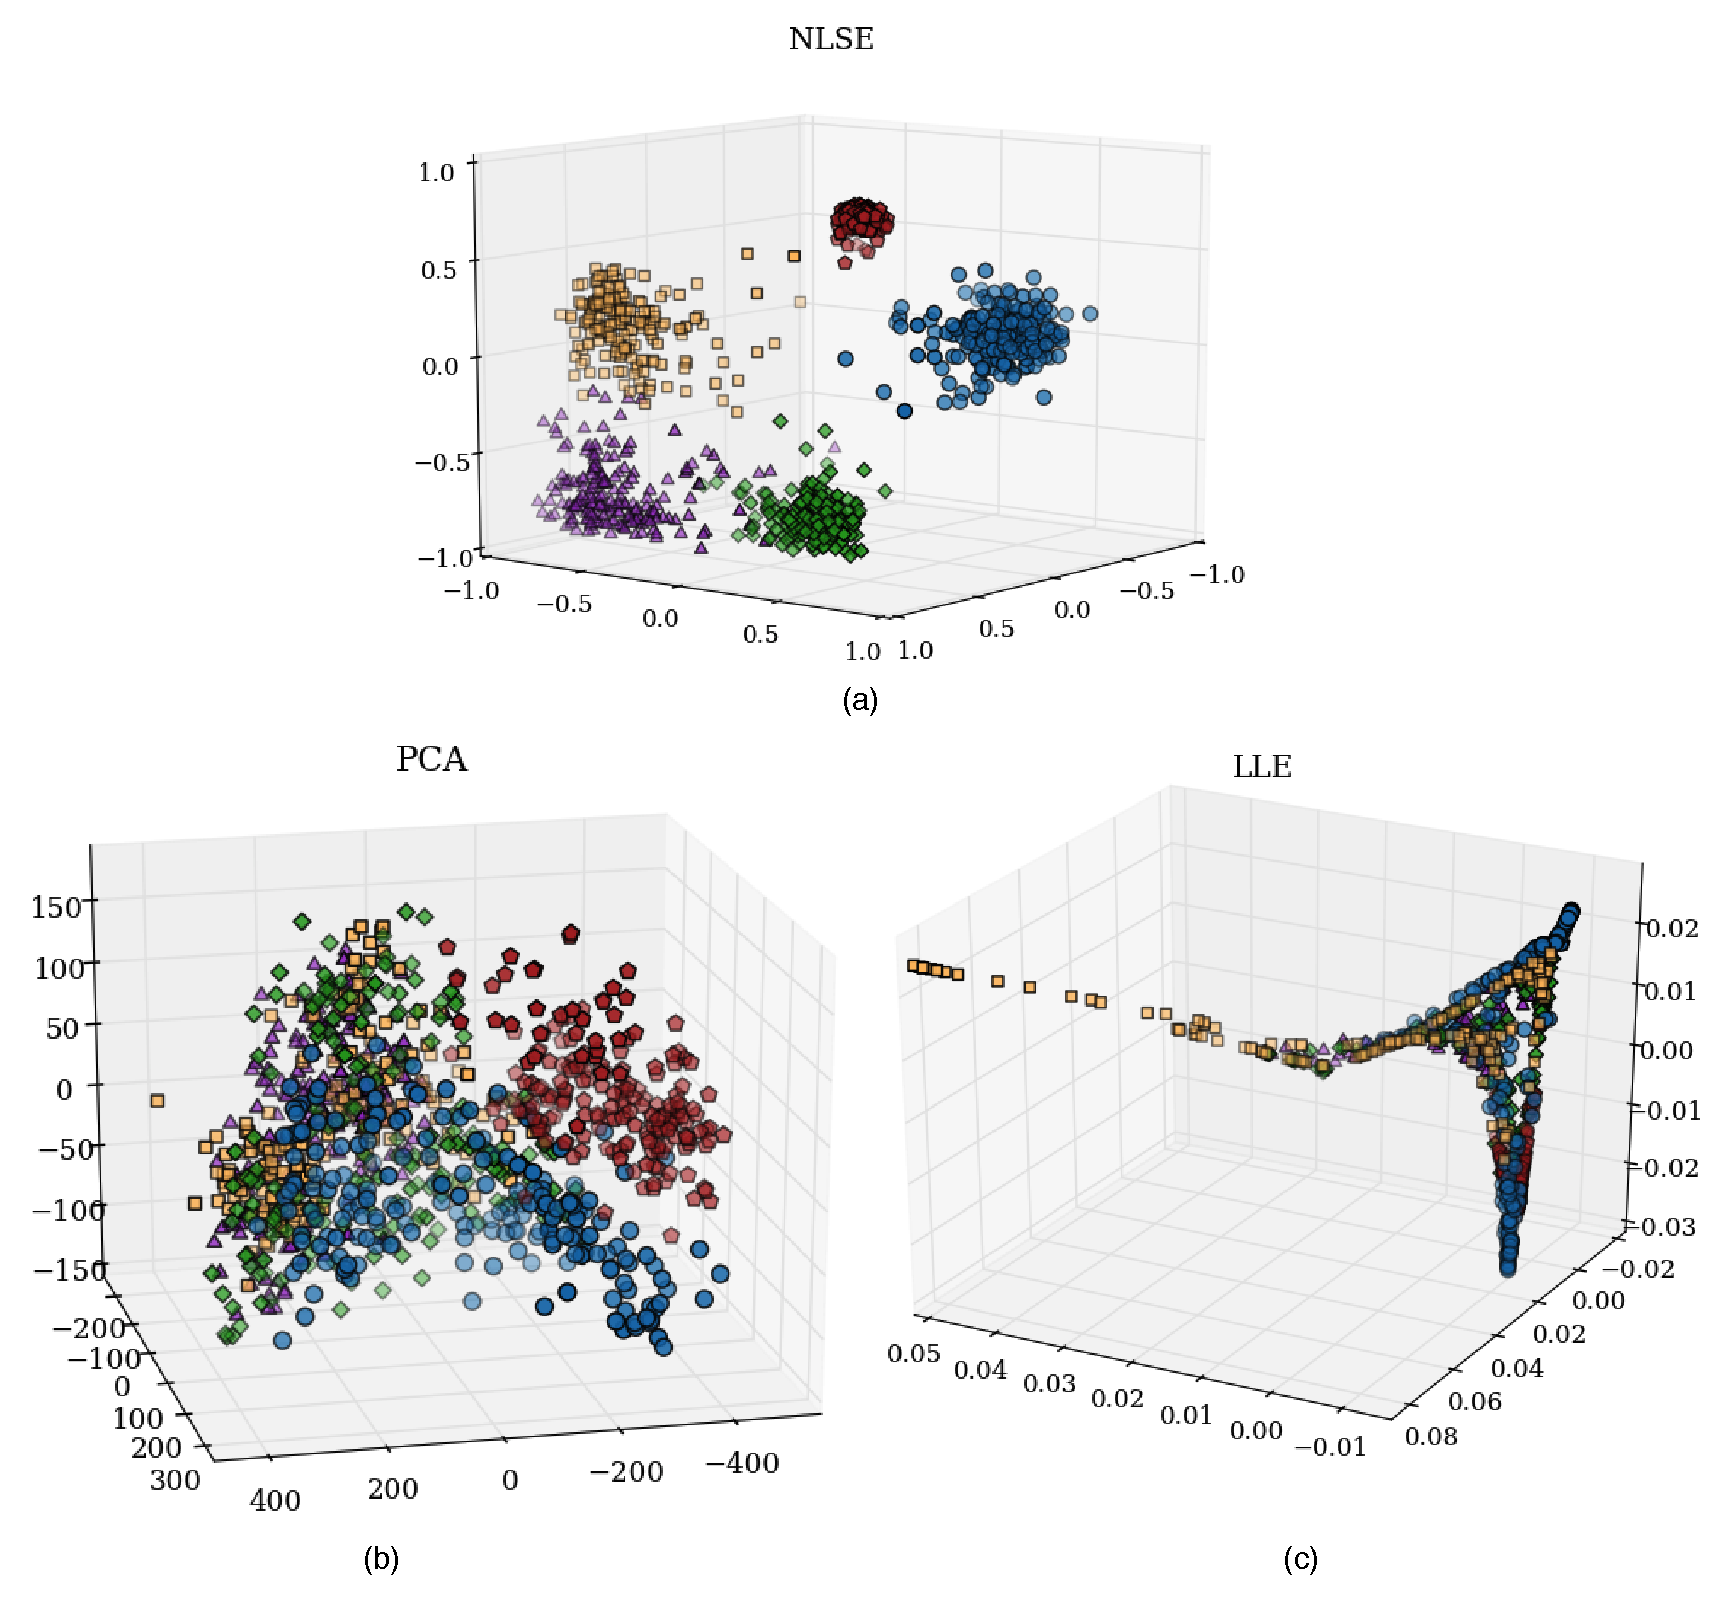
\includegraphics[width=\linewidth]{NLSECluster}
\caption[NLSE vs. PCA vs. LLE instrument clusters]{Output feature spaces generated by (a) NLSE, (b) PCA, and (c) LLE for Tuba (red pentagons), Oboe (green diamonds), Clarinet (purple triangles), Cello (blue circles), and Flute (yellow squares).}
\end{center}
\vspace{6pt}
\end{figure}

With the previous feature-learning discussion in mind, one may be quick to attribute the improved instrument discrimination seen in Figure 37 solely to NLSE being a supervised learning method as opposed to PCA and LLE, which are unsupervised dimensionality reduction algorithms. As a supervised method, NLSE has more data to use (specifically, the instrument labels) in learning an appropriate timbre space for instrument classification, whereas PCA and LLE are acting upon hand-crafted features (MFCCs). By utilizing labelled data to explicitly learn an appropriate feature space where such data is well-separated by label, Humphrey et al. have shown that supervised feature-learning methods can be superior to unsupervised methods applied to hand-crafted features. However, this says nothing about how feature-learning methods like NLSE compare to supervised dimensionality reduction techniques on hand-crafted features that are designed to provide good discriminatory power. Humphrey et al. also showed NLSE's superiority to these methods for generating an objective timbre space by comparing the NLSE-learned space to the space formed by applying linear discriminant analysis (LDA) on MFCCs \cite{humphrey2013feature}. A comparison of these spaces is shown in Figure 38.
\begin{figure}[h!]
\vspace{24pt}
\begin{center}
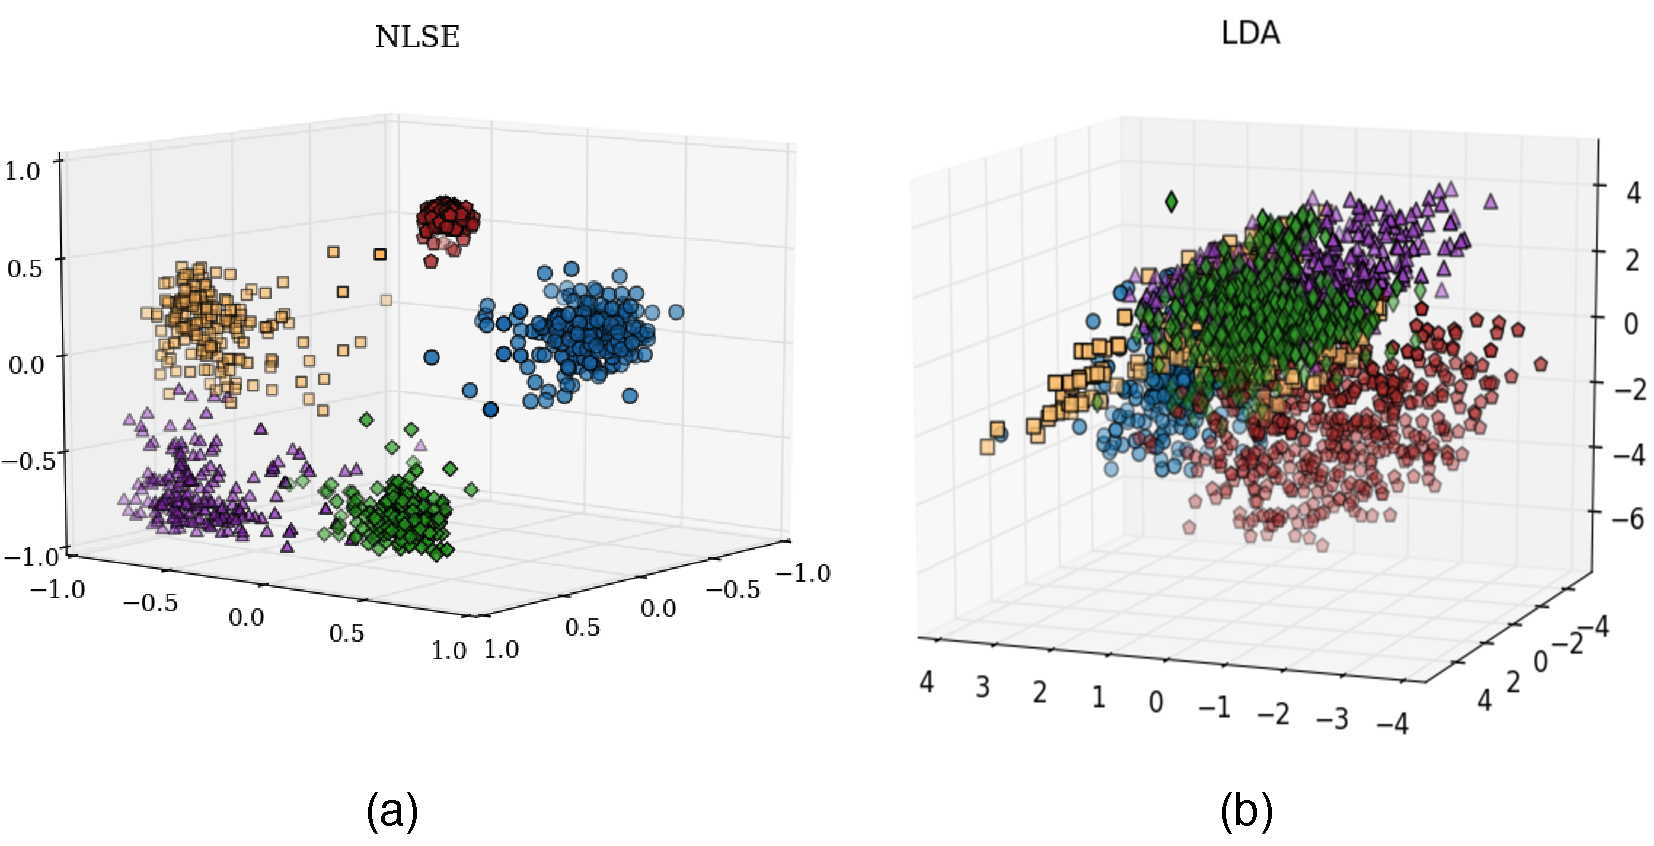
\includegraphics[width=\linewidth]{NLSECluster2}
\caption[NLSE vs. LDA instrument clusters]{Output feature spaces generated by (a) NLSE and (b) LDA for Tuba (red pentagons), Oboe (green diamonds), Clarinet (purple triangles), Cello (blue circles), and Flute (yellow squares).}
\end{center}
\vspace{6pt}
\end{figure}

NLSE clearly has better discriminatory power than LDA for instrument classification. This is important because it provides a comparison of two supervised learning methods: one that learns its own features (NLSE) and low-dimensional mapping into a semantically meaningful space and one that relies on the input of hand-crafted features (LDA) in order to learn a successful low-dimensional mapping. For this reason, we have chosen to use projections in the NLSE timbre space to represent instantaneous timbre features.

\vspace{12pt}
\subsection{Timbral Similarity}

In order to define an objective fitness function to measure the subjective nature of timbral similarity, we can look to a large body of work dedicated to the subject, originating within the genre recognition literature.

In early genre recognition systems, the typical timbral similarity measure employed was the calculation of KL-Divergence between GMMs of timbre features, as used by Pampalk \cite{Pampalk:2006pr}. The primary weakness of this often-used metric is that it ignores information about the temporal evolution of timbre. This information is thrown away when modeling the observed series of timbre feature vectors with a GMM probability distribution. 

The reliance of timbral similarity on timbral evolution trajectories is well-supported and fits in line with an objective timbre space representation (which we have adopted in this study). Toiviainen et al. note that a major component of the perception of timbre and measuring timbral similarity is the time-varying spectral envelope of sound \cite[p.225]{Toiviainen:1998hs}. This is further supported by Caclin et al. and also separately noted by Ciglar in more recent studies \cite[p. 1]{Caclin:2005il} \cite[p. 4]{Ciglar:2009uf}. Thus, appropriate timbral similarity models will measure similarities (i.e. the inverse of semantically relevant distances) between trajectories of perceptually relevant timbre features. 

While previously discussed research has attempted to incorporate temporal information into the features themselves (this is known as early fusion), other research has focused on incorporating temporal information into the classifier (known as late fusion) \cite[p. 500]{Meng:2005fx}.

For example, Flexer, Pampalk, and Widmer model similarity using a hidden Markov model (HMM) instead of a GMM \cite{Flexer:2005sw}. In describing their decision, they note that ``aspects like spectral fluctuation, attack or decay of an event cannot be modeled without respecting the temporal order of the audio signals'', which the GMM does not do (2005, p. 1). HMMs allow one to model time-varying timbral data using probability density functions representing locally stationary timbre and transition probabilities between those stable states (2005, p. 2). Thus, the temporal variation in timbre is directly incorporated into the model. However, in most implementations, first-order HMMs are used (due to their computational efficiency in comparison to higher order models), which retain only the temporal information regarding how neighboring feature vectors are ordered. This combined with the fact that this is a probabilistic mode, means that some information about the temporal evolution is lost. However, one would expect this to result in a much more adept model at calculating timbral similarity. Flexer et al. found, however, that this model did not achieve significant gains in genre classification performance (p. 5). This does not necessarily mean that HMMs do not provide any significant gains in generating semantically meaningful timbre distance measurements however, since genre classification performance is an indirect and imperfect measure of timbral similarity. It simply means that the temporal information provided by HMMs is not useful for genre recognition.

Jehan, in his dissertation, calculates similarity between perceptually processed spectral data using dynamic time warping (DTW) \cite[p. 70]{Jehan:2005fy}. By aligning the feature data between two feature vector sequences, one is able to account for slight time warpings and/or shifts between the sequences, allowing for a simple Euclidean distance calculation between aligned sequence vectors in order to calculate similarity. Jehan also incorporates the importance of the attack towards timbre perception directly into the DTW algorithm by dynamically weighing the path with a half-raised cosine function \cite[p. 71]{Jehan:2005fy}. While DTW retains virtually all of the temporal evolution information of a timbre feature sequence, it has an undesirable time-complexity. However, recently an O(N) variant of DTW, called FastDTW, that restricts the warp path based on reasonable assumptions has been developed \cite{Salvador:2004et}.

Late fusion similarity models like the HMM or DTW are a step in the right direction away from GMMs. However, other models should be investigated as well. As previously noted, low-order HMMs only retain short-time temporal information, and, while the DTW retains virtually all of the temporal evolution information in a sequence of timbre features, there may be examples where robustness to slight time warping or shifting is not enough to align two sequences that are semantically similar. For example, if two sound files contain the same distinct, repetitive timbral gesture, but one file contains a larger number of repetitions than the other, DTW will be unable to globally align them and therefore will consider them timbrally dissimilar.

Our approach, like DTW, also retains the temporal evolution of timbre by calculating similarity directly between two sets of timbre feature sequences. It provides similar results to direct Euclidean distance between feature vectors if the sounds compared are time aligned and not time warped and similar results to DTW if time warped and/or not time aligned. It additionally provides an appropriate similarity measure for when either a different number of repetitions are present in the sounds being compared, when timbre subsequences are re-arranged, or when two sounds' timbre curves only partially overlap - after some alignment and local warping - but diverge otherwise. The motivation for our approach begins by looking back at our objective timbre space.

Given the NLSE-learned timbre features we have chosen to use, our task is to develop a measure of timbral similarity for time-varying timbres in the space these features define. Timbres that do not vary over $N$ time-frequency patches will only occupy a small region or point in this space. The calculation of timbral similarity between static or near-static timbres of this sort can simply be approximated using the Euclidean distance between the individual distribution centers since the space is trained for this distance metric to be semantically meaningful (see Figure 39). 
\begin{figure}[h!]
\vspace{24pt}
\begin{center}
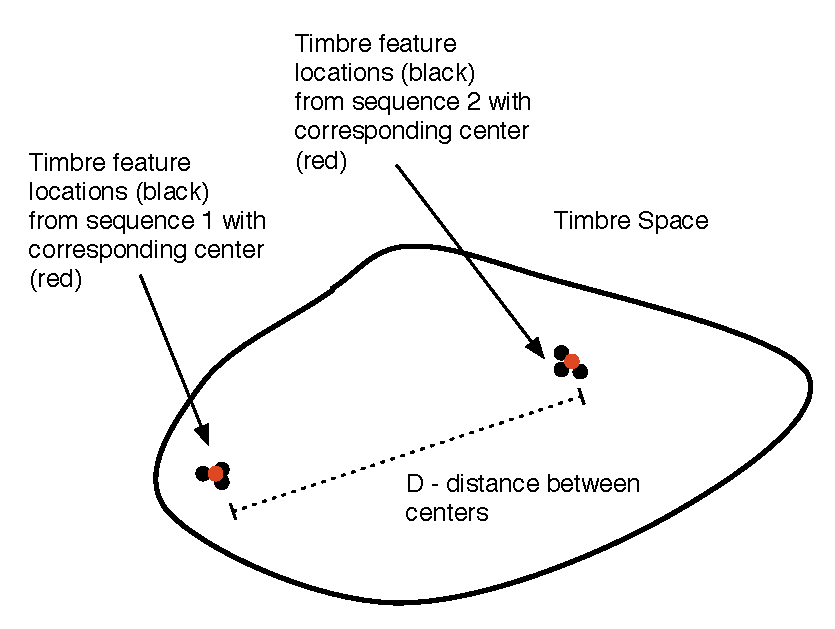
\includegraphics[scale=0.8]{TimbreDistance1}
\caption[Timbre distance between centers]{Timbral similarity between two sequences of time-frequency patches approximated using the distance between their centers.}
\end{center}
\vspace{6pt}
\end{figure}

However, the calculation of timbral similarity becomes more complicated once both sounds contain timbral variation, which will correspond to two different paths traced out in timbre space away from the regions in which they started. The task then becomes measuring similarity between these paths (see Figure 40).
\begin{figure}[h!]
\begin{center}
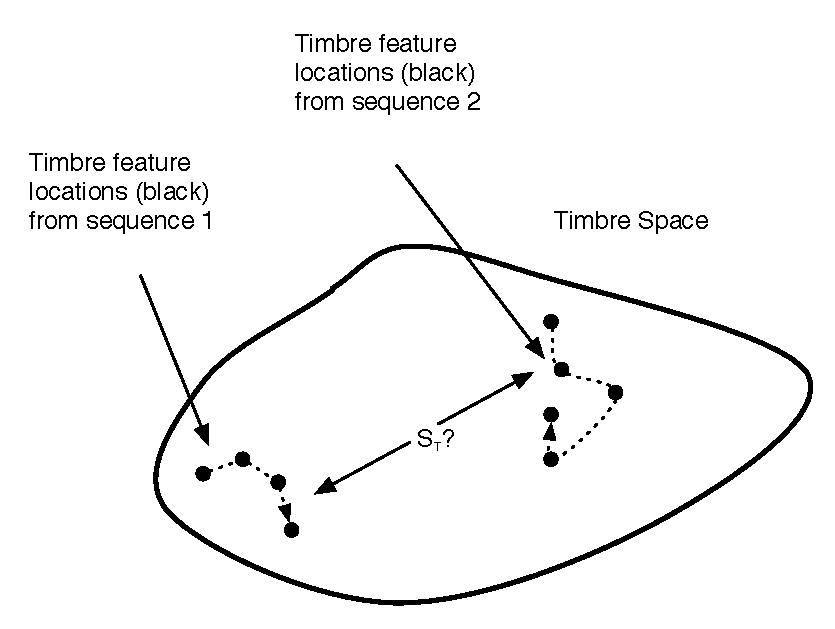
\includegraphics[scale=0.8]{TimbreDistance2}
\caption[Timbre distance between curves]{How does one calculate the similarity or distance between two curves in timbre space that are not well localized?}
\end{center}
\vspace{6pt}
\end{figure}

Since points in timbre space will occur at regular discrete intervals in time, the paths actually represent discrete sequences of timbre points. Therefore, the question we must answer is: ``How should one measure the timbral similarity between two discrete sequences (possibly having different lengths) of timbre feature vectors?" If we only allowed comparisons between sequences of equal length (an undesirable restriction), a common solution would be to line up points in the two feature vector sequences, calculate the Euclidean distance between the pairs of lined up points, sum all distances, and take the inverse of the result (referred to as the \textit{aligned-Euclidean} method going forward):
\begin{equation}
S_T = \frac{1}{\sum_{i=1}^{M}\sqrt{\sum_{j=1}^{N}(Z_{ij}^1 - Z_{ij}^2)^2}}
\end{equation}
where $Z^1$ and $Z^2$ represent the two sequences of timbre feature vectors to compare (obtained by processing time-frequency patches through our trained CNN architecture), N is the dimensionality of the timbre feature space, and M is the length of each sequence.

However, even after imposing the restriction of equal sequence lengths, there are many examples where this measure will break down. For example, if one takes two copies of the same exact sound and applies a simple linear time shift to one (i.e. a delay), the suggested similarity calculation could result in labeling the two sounds as being very distant (see Figure 41).
\begin{figure}[h!]
\vspace{24pt}
\begin{center}
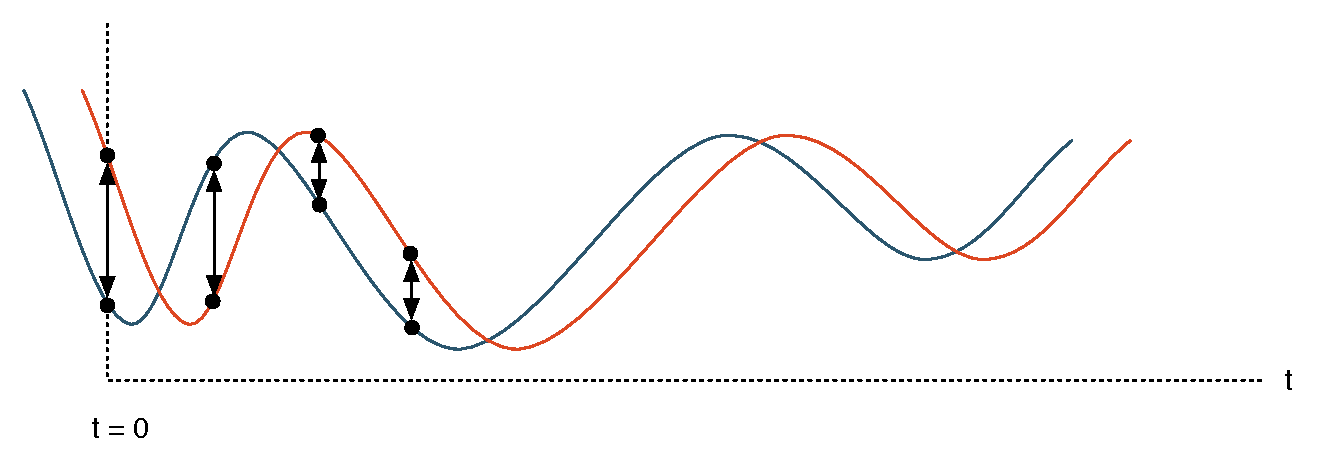
\includegraphics[scale=0.6]{TimbreDistance3}
\caption[Timbre distance between time-shifted curves]{An example of how a simple temporal shift of the exact same curve can result in non-negligible distance calculations between corresponding points in the resultant discrete sequences.}
\end{center}
\vspace{6pt}
\end{figure}

Slight time warpings of one sound compared to the other would also result in an incorrect assessment (see Figure 42). It is for this reason that Jehan uses Dynamic Time Warping (DTW) when calculating similarity over sound segments \cite{Jehan:2005fy}. The only difference between the problem he was addressing and ours is the time scale on which similarity is being computed.
\begin{figure}[h!]
\begin{center}
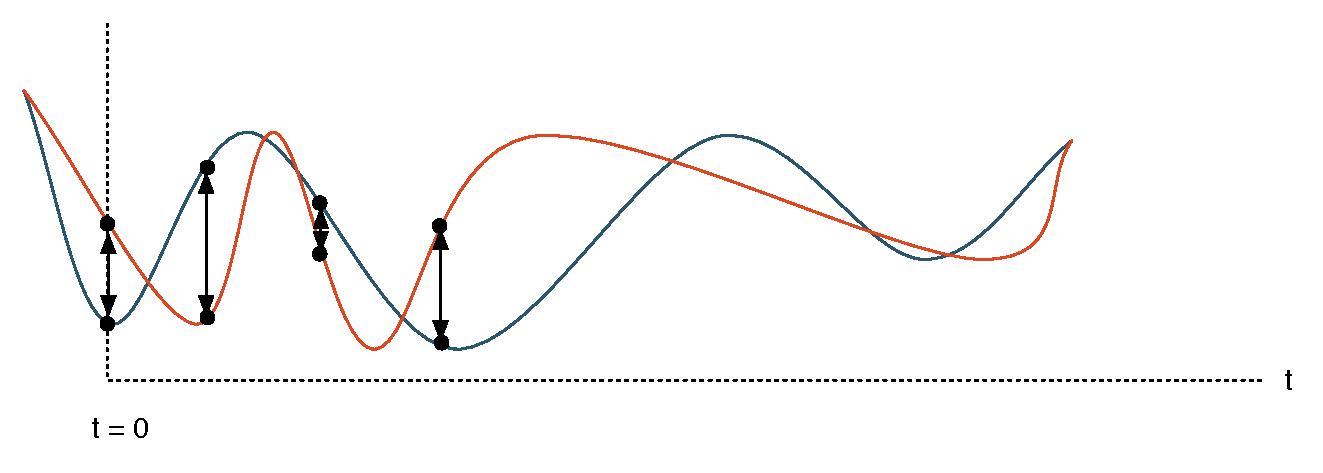
\includegraphics[scale=0.6]{TimbreDistance4}
\caption[Timbre distance between time-warped curves]{An example of how a temporal warping of the exact same curve can result in non-negligible distance calculations between corresponding points in the resultant discrete sequences.}
\end{center}
\vspace{6pt}
\end{figure}

DTW is a dynamic programming method that attempts to align the time scales over which two different sequences of data occur by finding the optimal warping path between those time scales. The DTW-distance is found by summing the distances over pairs of aligned points in the two sequences. Salvador and Chan provide a more detailed overview and a real-time implementation of a close approximation \cite{Salvador:2004et}. In Figure 43, we provide a diagram of the best warping path given the two sequences from the example in Figure 42.
\begin{figure}[h!]
\begin{center}
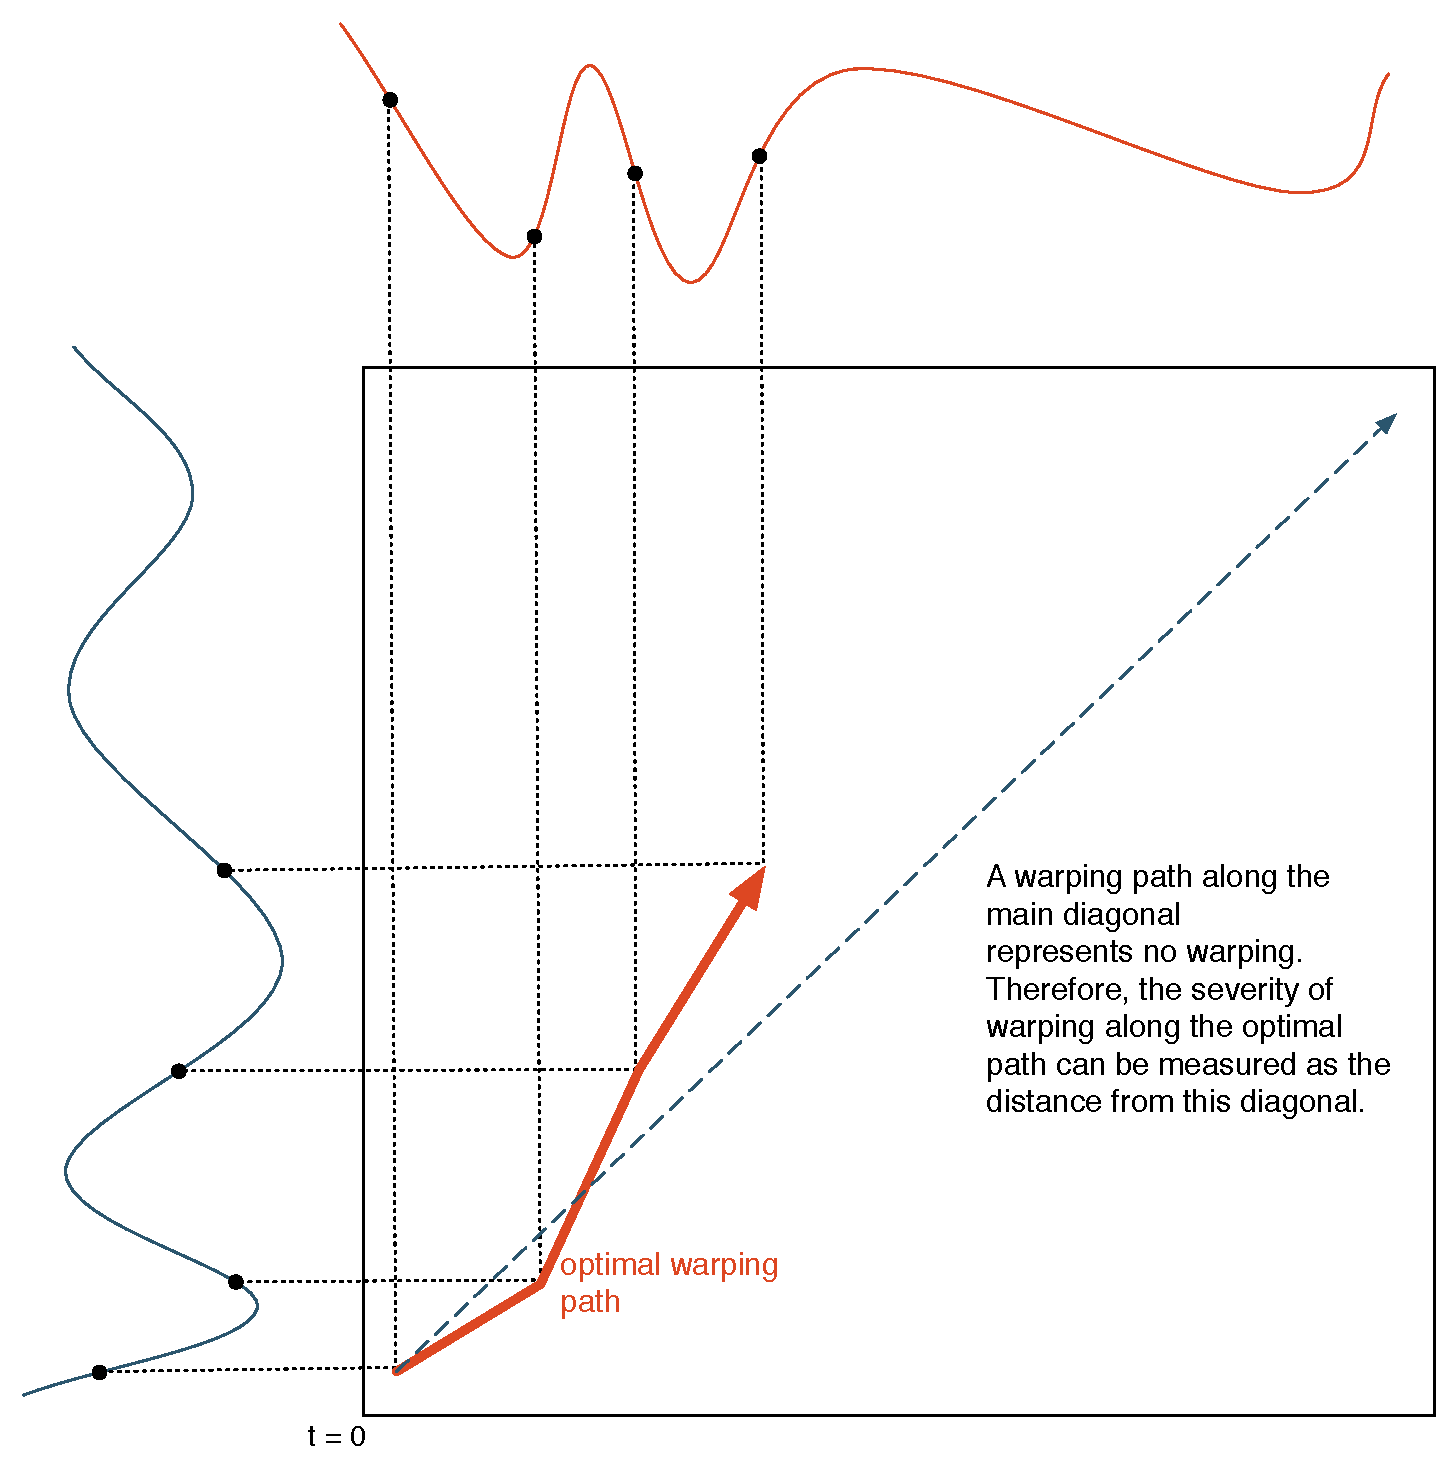
\includegraphics[scale=0.5]{DTWExample}
\caption[Optimal warping path]{The optimal warping path between the two sequences from Figure 42 is shown.}
\end{center}
\vspace{6pt}
\end{figure}

In this example, the sequences look identical after alignment (exemplified by the aligned points in the figure). Thus, accumulating distances between aligned pairs would result in a very small sequence distance and consequently a very high similarity.

DTW can be performed on sequences that have different lengths, which obviates the need for the same-length restriction required for the aligned-Euclidean measure. If two similar timbral sequences are not time shifted or time warped, but instead could accurately be described using the aligned-Euclidean distance measure, DTW will most-often return a warping path that is near linear (i.e. very close to the main diagonal) so that the DTW result will match the aligned-Euclidean result. One disadvantage of DTW is that it can be more generous to sequences that were generated from very dissimilar content than the aligned-Euclidean method because it returns the absolute best alignment based on what warping path maximizes similarity. However, DTW will most often produce better alignments and corresponding similarity scores for sequences that are naturally similar under warping than for sequences that are not, so this issue is not too significant, especially when one is most interested in relative comparisons.

While DTW provides a metric that is invariant to time shifts, warpings and other temporal distortions (e.g. random sample deletion and random extension of static timbral content), there are situations in which it is not sufficient. The major drawback of DTW is that it requires that the first and last vector of each sequence are aligned and that both sequences move forward in time from beginning to end. In other words, it can only search for the best global warping path between two sequences. This is problematic given two sequences that are produced by the same object, but that contain a different amount of similar repeated subsequences. An example in our problem domain would be if we had two audio clips of the same bird chirping and breathing (labelled $A$ and $B$, respectively), with one clip containing three chirps followed by one breath ($AAAB$) and the other containing two chirps, one breath, and then another two chirps ($AABAA$). DTW would only search for paths that would align the two global sequences (likely resulting in a linear path through the first two $AA$s in each sequence and then stumbling to find an appropriate match to the third $A$ in the first sequence) and would fail to find an appropriate path to consider these two sequences similar, even though they in fact contain timbral subsequences that are almost exactly the same and that follow a similar sequencing of several $A$s followed by a $B$ \cite[p. 1143]{serra2008chroma}.

One solution is to eliminate the global alignment requirement of DTW. Serr\`a et al. propose a method they call \textit{dynamic programming local alignment} (DPLA) that leverages both principles of DTW and the \textit{Smith-Waterman} algorithm (a technique used in molecular biology that optimizes a similarity measure by comparing subsequences of all possible lengths) to find the longest similar subsequence between two sequences \cite{serra2008chroma}. DPLA uses only the data from the most-similar subsequence to calculate a similarity measure for purposes of cover song identification. In their problem domain, this measure works well because it is completely natural for cover songs to contain segments that are wholly different from the original and which therefore should be ignored as long as there is a long enough segment/subsequence that matches well with the original. In other words, an original song with structure $ABABC$ may have a cover with structure $BAADE$ (In this example, letters refer to subsequences of time-frequency patches that may or may not repeat within the overall sequence). The dramatic structural changes found in moving from original to cover should not interfere with the detection of this cover. All that matters in this case is a very strong correlation between a similar subsequence that both original and cover share. Thus, these sequences should be considered similar and DPLA labels them as such. This is not an optimal similarity measure for timbre however, as a brief moment of a similar sonic texture in two given sounds surrounded by vastly different textures should not result in high timbral sequence similarity between the them. While we do not want to enforce a global warping when comparing two timbral sequences, we do want a measure that takes the global sequences into account.

Given this, our approach looks for the best sequence of local subsequence alignments, where subsequences may be repeated, internally warped, and placed out of order, but such transformations are penalized. We have decided to penalize these transformations because we believe that too much of any will disrupt the overall sense of timbre. Figure 44 shows a few examples of distorted sequences we would penalize.
\begin{figure}[!p]
\begin{center}
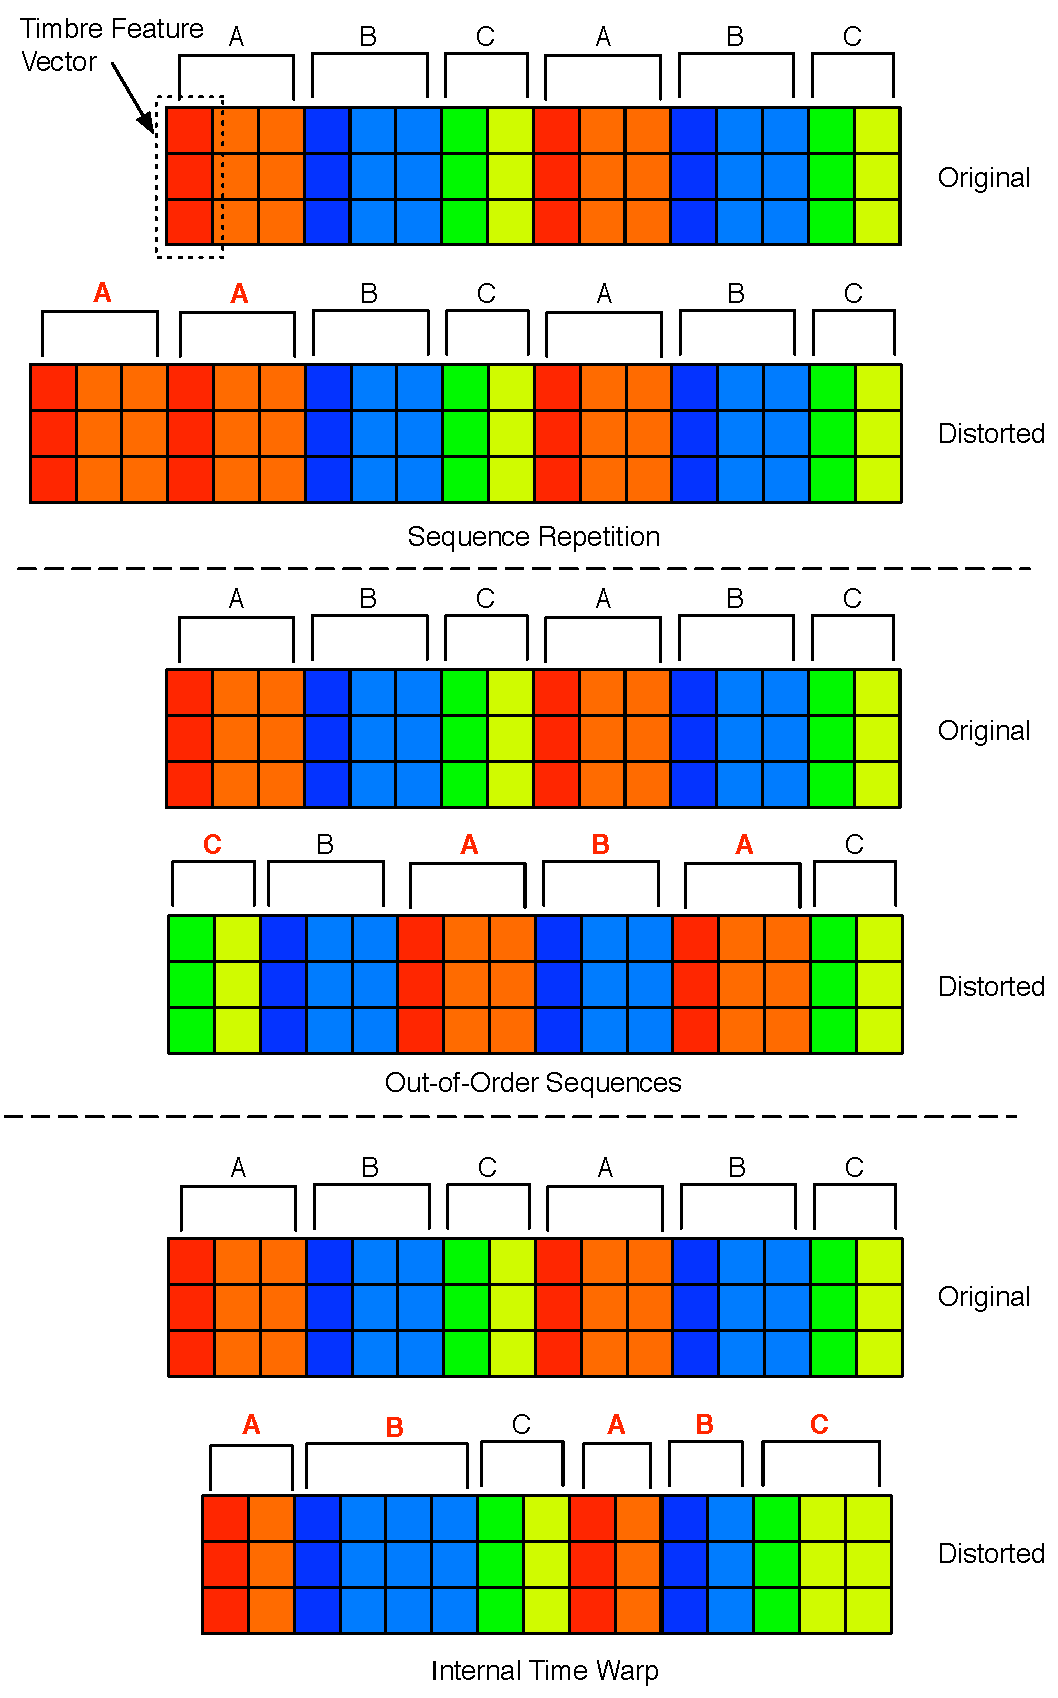
\includegraphics[scale = 0.6]{SequencePenalties}
\caption[Proposed sequence similarity penalties]{Distorted sequences that would incur penalties (with problematic subsequences labelled in red text). From top to bottom, subsequence $A$ is repeated, subsequences appear out of order, and subsequences are time warped.}
\end{center}
\vspace{6pt}
\end{figure}

In the top example, the first instance of the subsequence labelled $A$ is repeated in the distorted version. In the middle example, several of the various labelled subsequences in the original appear out-of-order in the distorted sequence. In the bottom example, the subsequences  in the distorted sequence are time warped with respect to the original sequence. All of these distorted sequences will incur penalties and consequently will not achieve perfect similarity scores using our approach.

An initial approach given the above could use a greedy algorithm that utilizes DPLA to find the longest common subsequence between sequences, removes those subsequences and repeats the process until an appropriate stopping criteria is met (e.g. the remaining sequence length after removing all paired subsequences is less than some threshold). A problem with this approach is exposed in the example shown in Figure 45. 
\begin{figure}[!p]
\begin{center}
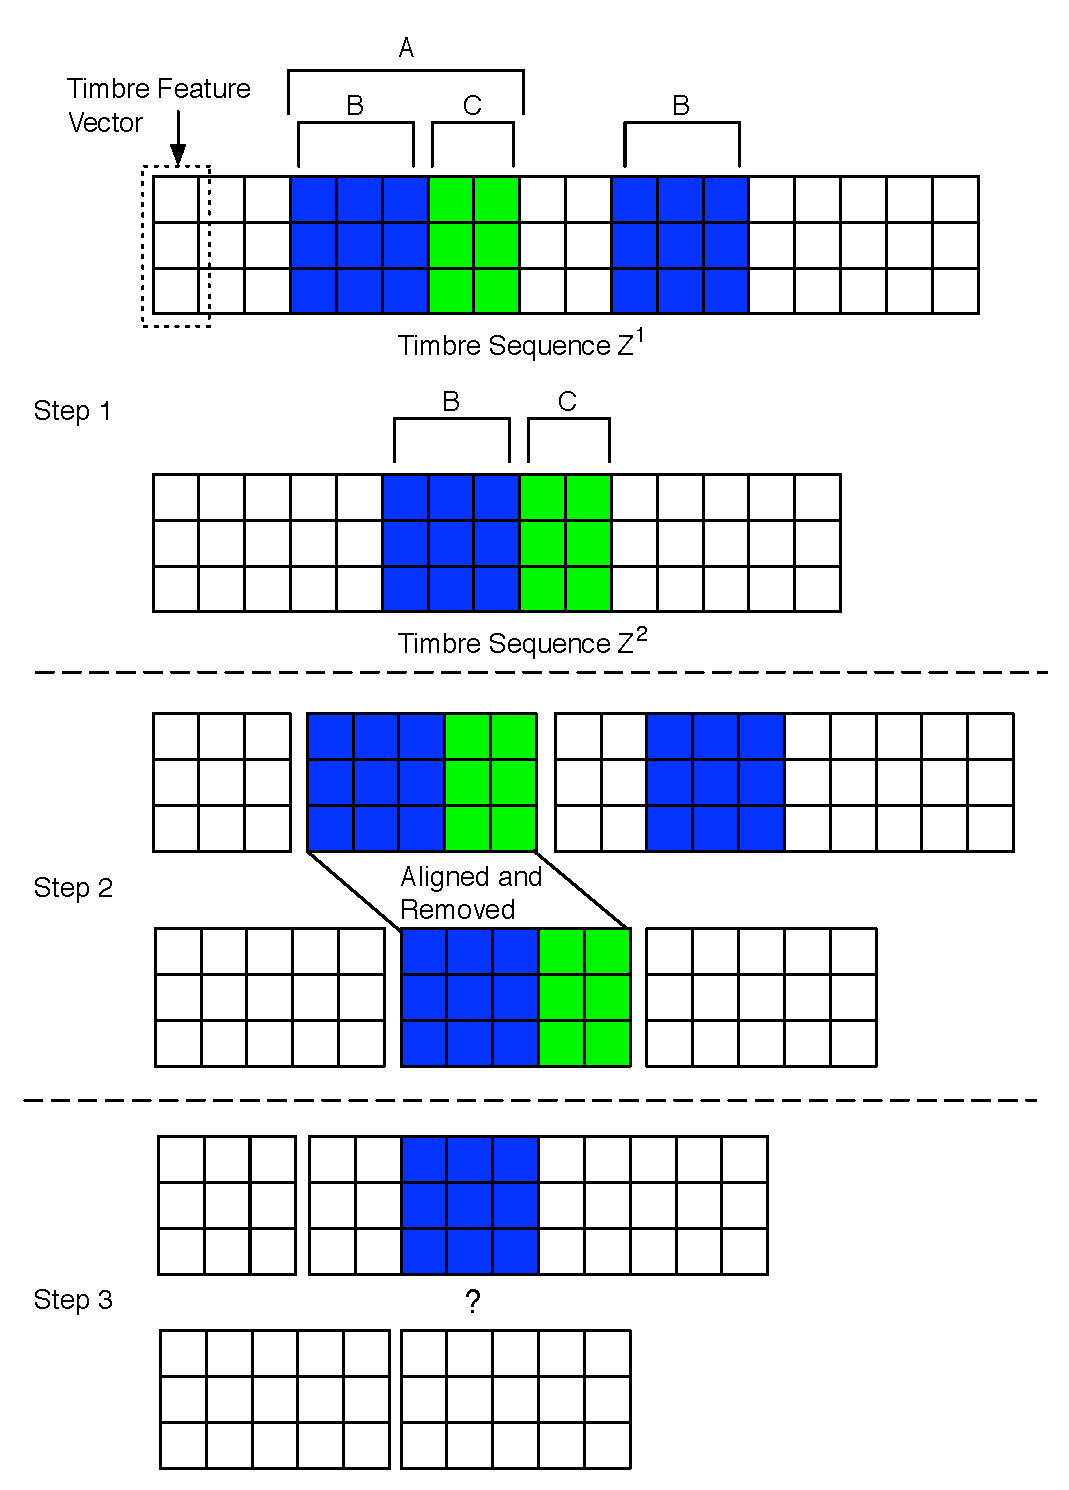
\includegraphics[scale=0.6]{GreedyMatching1}
\caption[Symmetric greedy removal after matching]{In step 1, we search for the optimal local alignment between the two sequences. Once we find that alignment in step 2, we remove the subsequences involved from further consideration. In step 3, we have left a repetition of subsequence B stranded without a corresponding match in the second sequence.}
\end{center}
\vspace{6pt}
\end{figure}

The first subsequence to be matched and removed in this example, $A$, is composed of two smaller subsequences, $B$ and $C$. By removing $A$ from both sequences as the first greedy step, the only instance of $B$ is removed from the second sequence. This leaves a repetition of $B$ in the first sequence that does not have a match in the second. The algorithm will therefore be forced to match the first sequence's remaining $B$ with a portion of the second sequence that may differ considerably, producing a poor similarity score.

This issue arises because of the greediness of the approach. By removing a subsequence from contention from one sequence that the other could re-use to find an appropriate alignment to another one of its subsequences (e.g. $B$ in this example), we have weakened our ability to fairly find the best combination of optimal local alignments. We have given preferential treatment to one sequence (that which does not require an aligned repetition of $B$) over the other. This situation can occur over a single set of two sequences in both directions, so it isn't a matter of determining which sequence to prefer in our search if we use this greedy approach. 

A slightly less greedy option is to only eliminate the aligned subsequences of one sequence while allowing re-use of the entire other sequence throughout the alignment process. In other words, we start by finding the best subsequence alignment between two sequences $Z^1$ (the superior) and $Z^2$ (the inferior), remove that subsequence from $Z^1$ (but not from $Z^2$) and then search for the best local alignment between the two left over pieces of $Z^1$ and the entirety of $Z^2$, continuing along until all of $Z^1$ is aligned to some part of $Z^2$ (see Figure 46(a)).

This method obviously is biased towards finding appropriate matches in $Z^2$ to all of $Z^1$ (and not vice versa), but can be made symmetric by repeating the process in the opposite direction (removing aligned subsequences of $Z^2$ along the way, but reusing any aligned segments of $Z^1$) (see Figure 46(b)). 
\vspace{12pt}
\begin{figure}[h!]
\begin{center}
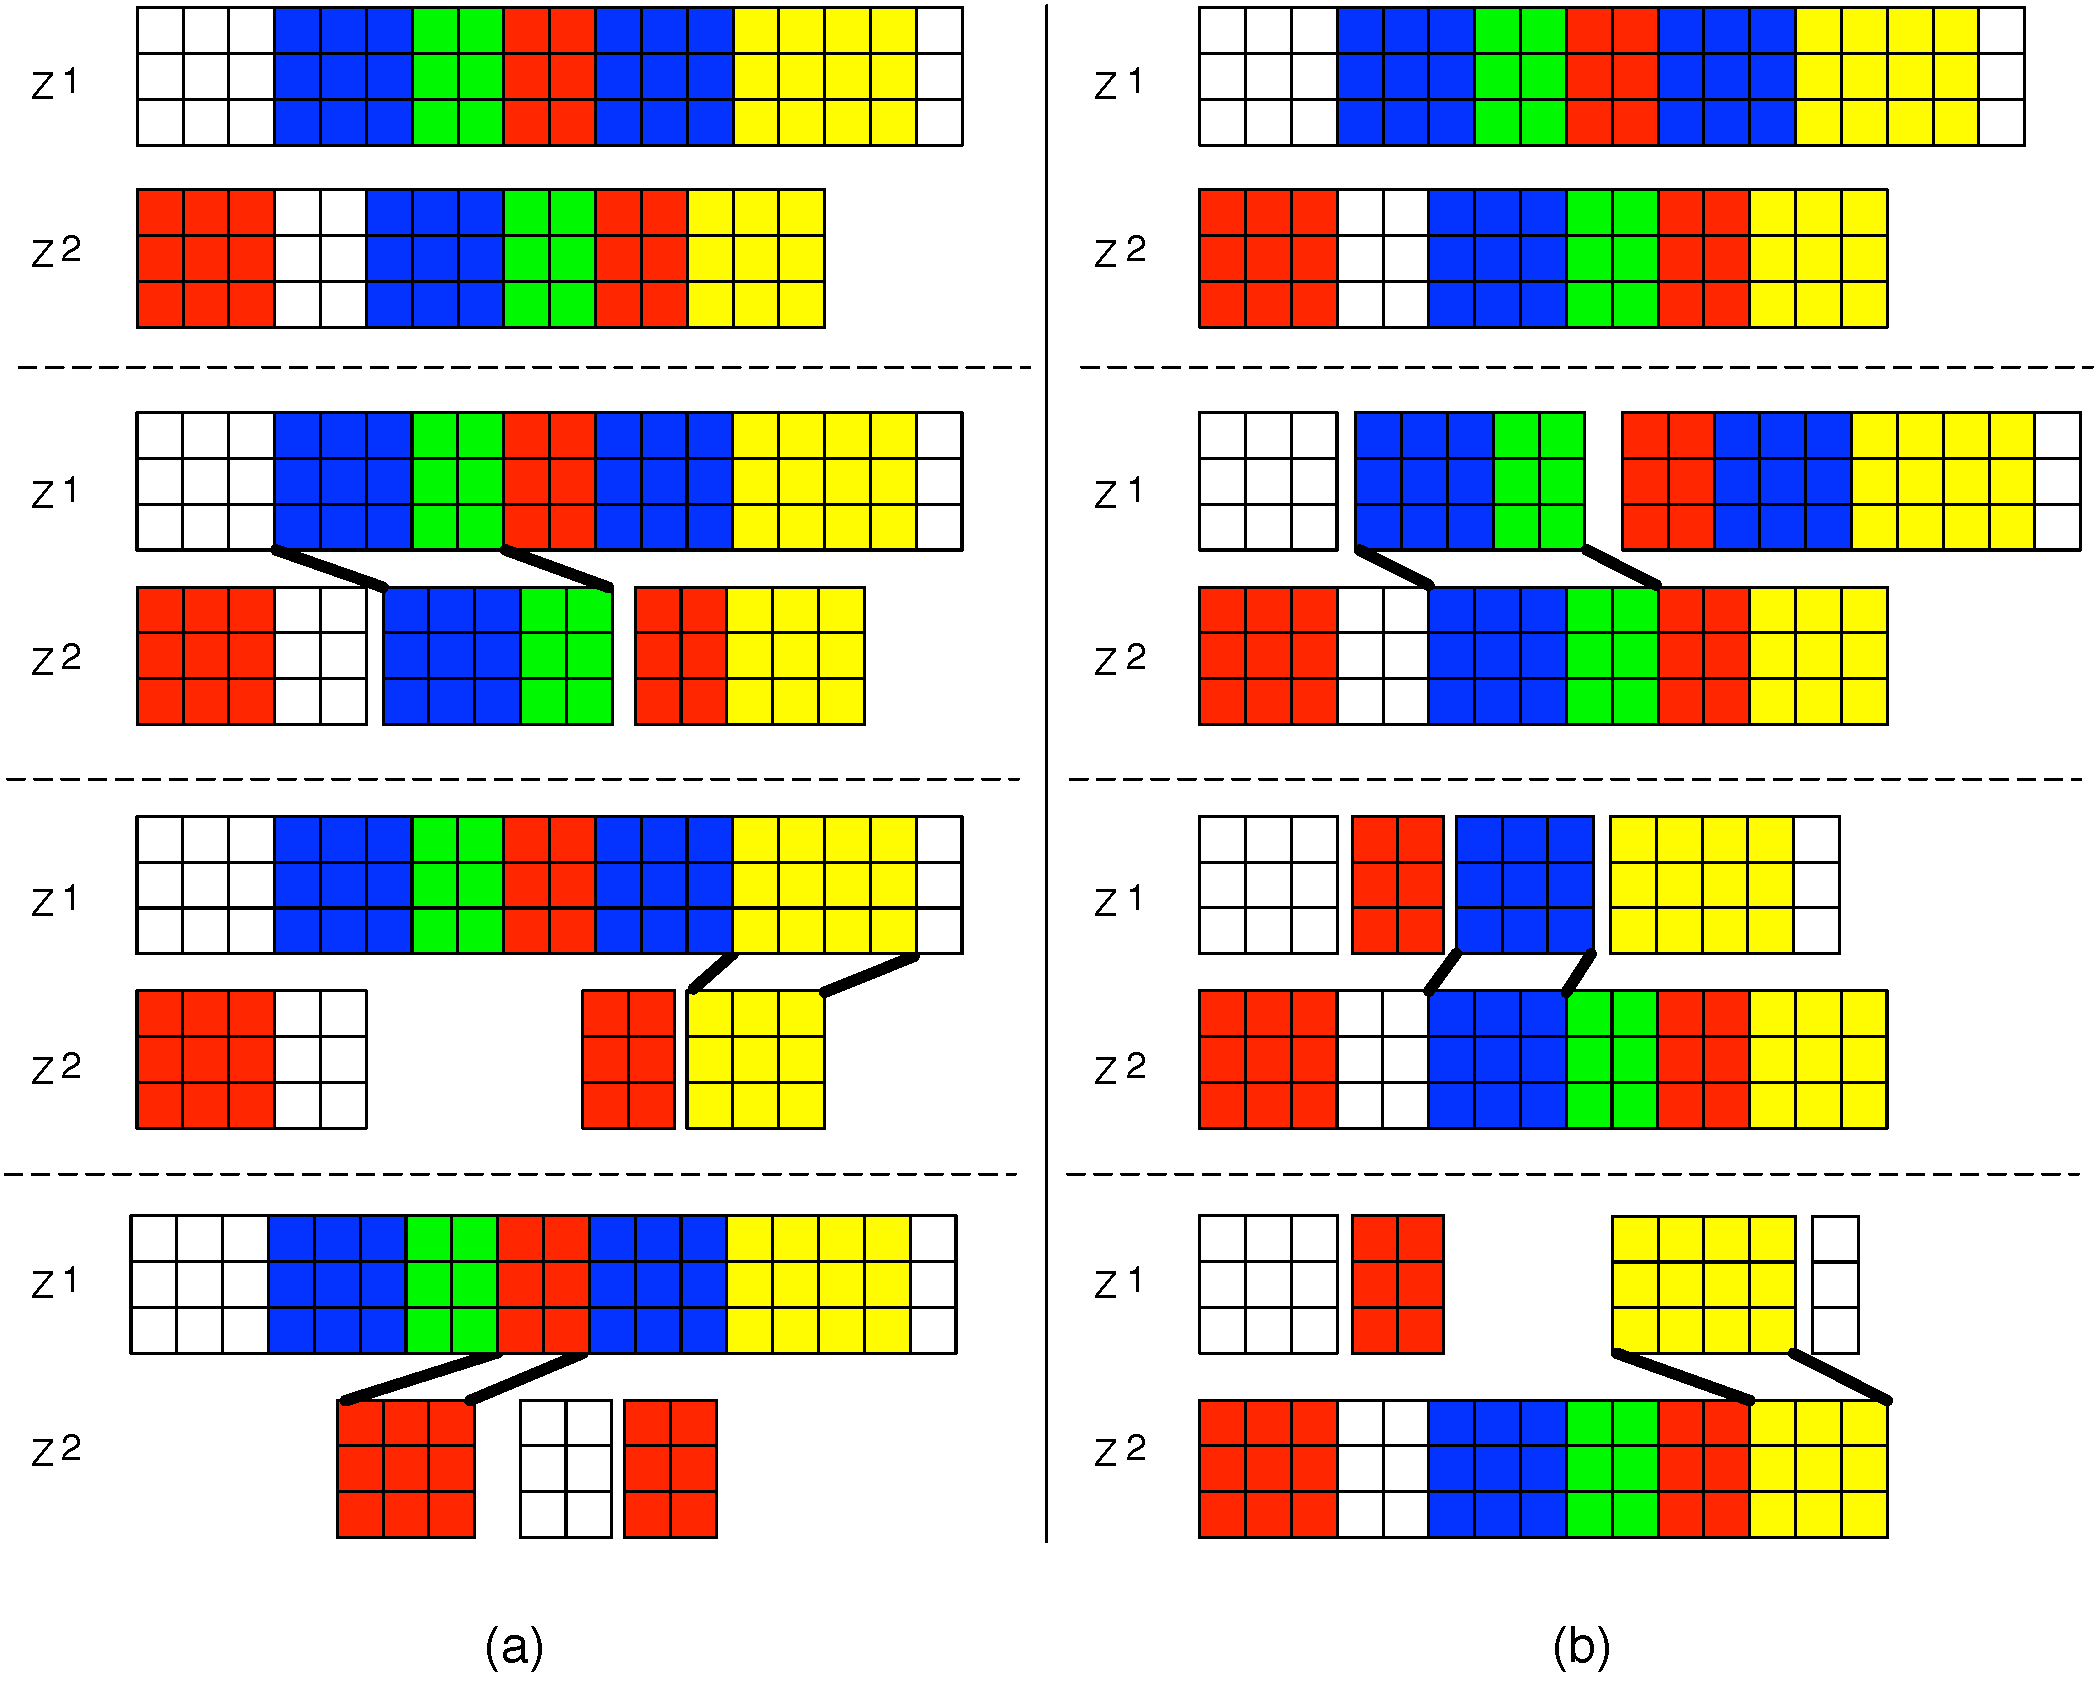
\includegraphics[width=\linewidth]{GreedyMatching4}
\caption[Asymmetric greedy removal after matching in both directions]{(a) The optimally matched subsequences of $Z^2$ are removed after they are found, while $Z^1$ remains intact to provide $Z^2$ with the ability to match numerous subsequences to the overlapping content in $Z^1$. (b) The optimally matched subsequences of $Z^1$ are removed after they are found, while $Z^2$ remains intact to provide $Z^1$ with the ability to match numerous subsequences to the overlapping content in $Z^2$.}
\end{center}
\vspace{6pt}
\end{figure}
The alignment combinations that are produced for each process can be used to calculate individual distance scores and then summed for a symmetric measure of similarity between both sequences:
\begin{equation}
S_T = \frac{2}{D_{SIC-DPLA}} \equiv \frac{2}{D_{IC-DPLA_{1\to2}} + D_{IC-DPLA_{2\to1}}}
\end{equation}
where $D_{SIC-DPLA}$ is what we call the \textit{symmetric iterative continuous DPLA} (SIC-DPLA) distance, $D_{IC-DPLA_{1\to2}}$ is what we will call \textit{iterative continuous DPLA} (IC-DPLA) distance calculated when treating $Z^1$ as the superior sequence (defined below) and $D_{IC-DPLA_{2\to1}}$ is the IC-DPLA distance calculated when treating $Z^2$ as the superior sequence.

The remaining question is how one calculates the SIC-DPLA distance based on a number of subsequence alignments that may or may not be ordered appropriately in time, may or may not overlap in one or both sequences (this including repetitions), and may or may not include the entirety of both sequences. All of these must be considered in determining an asymmetric global sequence similarity score before averaging this measure over the results of the process in both directions. To begin, we must briefly review both DPLA and the Smith-Waterman algorithm and discuss how we can leverage them for our problem domain.

As previously mentioned, DPLA utilizes the Smith-Waterman technique for performing local sequence alignment. The Smith-Waterman algorithm was first presented for the purposes of  finding ``maximally homologous subsequences among sets of long sequences...in molecular sequence analysis''  \cite[p. 196]{smith1981textordfeminineidentification}. This problem domain differs from ours (as well as that of Serr\'a et al.) in that molecular sequences contain a fixed set of discrete values. This is an important distinction, because the Smith-Waterman technique typically is used in a problem domain where one will often find exact subsequence matches within a sequence. In its basic form, it takes a binary similarity matrix as its input based on this assumption, where one of the possible values represents \textit{sameness} and the other, \textit{difference}.

Serr\'a et al. look for local sequence alignments using the principles of Smith-Waterman, and in order to fit their problem to one that is readily handled by that technique, they generate a binary similarity matrix between \textit{harmonic pitch class profile} (HPCP) vectors - a standard, continuous-valued feature in the domain of cover song identification - by using a thresholded similarity function with binary output \cite{serra2008chroma}. If two HPCP vectors are similar enough, this threshold function considers them the same and if they are not, different. Serr\'a et al.'s ability to transform their problem into one that looks typical for Smith-Waterman allows them to use the technique almost \textit{out of the box}.  However, the goal of most problems utilizing the Smith-Waterman algorithm is slightly different from ours (in that we do not only consider exact matches between timbre vectors as being similar). Consequently, we have decided not to try to transform our problem into one its standard implementation understands, but instead we have chosen to transform its standard implementation to one that fits our problem.

The Smith-Waterman algorithm assigns a positive value to two similar vectors and a negative value to two dissimilar vectors, so that ``these values have an average for long, random sequences...of zero'' \cite[p. 196]{smith1981textordfeminineidentification}. This is important because we will be looking at the cumulative sum of these values over subsequences of vectors to determine whether they align well. If the cumulative sum is greater than $0$, we can assume this is not by chance and that these two subsequences should be aligned. In the standard implementation, pairs of vectors can only be labelled \textit{similar} or \textit{dissimilar} and therefore will only take on either a single positive value or a single negative value. By comparing all pairs of vectors in two sequences this way, one obtains a binary similarity matrix, $S$, where its elements $s_{ij}$ are positive if vector i from the first sequence and j from the second sequence are similar and a negative value if they are dissimilar.

The standard calculation of a binary similarity matrix is not required for Smith-Waterman to function appropriately. The important part of Smith-Waterman - and that which separates it from something like DTW - is that it creates inherent segmentation boundaries for optimally aligned subsequences due to its accumulation of both positive and negative similarity values and the requirement that its alignment matrix is non-negative. The non-negativity of the alignment matrix means that alignments can begin anywhere and that any low-scoring alignment which precedes it will not affect it (since negative alignment values are not allowed and therefore thresholded to zero). Thus, the value of zero near a positive element in the alignment matrix is a marker that represents the starting point of where two subsequences begin to align well. As already stated, the technique looks for subsequences that, over their length, accumulate positive similarity values (as will be discussed in detail below). Once these accumulations start to trend negatively, the alignments can be considered complete and local subsequence alignment boundaries are defined (the start by a value of zero and the end by a local maximum in the alignment matrix). Therefore, continuous valued similarity matrices may be used in Smith-Waterman as long as the elements can take both positive and negative values and as long as we keep the requirement that the alignment matrix is non-negative.

In our problem domain, we have already defined a similarity measure over individual timbre feature vectors that exist in our learned NLSE output space: Euclidean distance. We know this measure is appropriate because we specifically trained our pairwise CNN architecture using Euclidean distance as the cost function and tested the space's instrument clustering ability using a kNN classifier that utilized Euclidean distance as its metric. Thus, we simply need to translate our Euclidean distance to a similarity measure that can take both negative and positive values in order to apply the Smith-Waterman algorithm. 

If we considered some boundary distance $\epsilon$ a distance from one timbre feature vector within which all other feature vectors are equally considered the same and outside of which all other feature vectors are considered different, we would be left with a binary similarity measure, which could be immediately input into the standard Smith-Waterman algorithm. However, this binary squashing operation is unnatural in that we want to be able to represent many gradations of timbral similarity and labeling all timbres within some radius of timbre space as equivalent does not allow this. Instead, we have chosen to linearly scale our distance measure into a range of $-1.0$ to $1.0$ so that the appropriateness of the Euclidean distance we learned is maintained in the measure. Our learned timbre space transformation takes time-frequency patches and reduces them down to points in 3-space within the cube enclosed by the range $[-1.0,1.0]$ in each of its three dimensions. Therefore, the maximum distance between two timbre points (i.e. the distance between two maximally dissimilar timbres) is $\sqrt{3*2^2} = 2\sqrt{3}$. This distance should correspond to a similarity score of $-1.0$ while the minimal distance between two timbre points (i.e. the distance between maximally similar timbres), $0$, should correspond to a similarity score of $1.0$. If all intermediate distances are linearly scaled between these two values we are left with the following similarity calculation between any two timbre vectors $Z_i^1$ and $Z_j^2$:
\begin{equation}
s(Z_i^1, Z_j^2) = 1.0-\frac{\sqrt{\sum_{k=1}^{N}(Z_{ik}^1 - Z_{jk}^2)^2}}{\sqrt{3}}
\end{equation}
If we apply this formula to all pairs of timbre feature vectors in the two sequences $Z^1$ and $Z^2$ and place the resultant $s(Z_i^1, Z_j^2)$ values into the elements $s_{ij}$ of a similarity matrix $S$, we can input this to the Smith-Waterman algorithm to find the best local subsequence alignment within the two sequences. We call this the \textit{continuous DPLA} (C-DPLA) variation going forward to separate it from the standard version which generates a binary similarity matrix as input to the Smith-Waterman-like algorithm Serr\'a et al. use.

The standard Smith-Waterman algorithm builds an alignment matrix, often labelled $H$ \cite{smith1981textordfeminineidentification}. Typically, gaps and deletions are allowed, but penalized. The concepts of gaps and deletions really only make sense when the problem domain is such that individual elements cannot be repeated (as they can in DTW), but instead may either be separated by gaps or may be skipped over (i.e. deleted). For example, given sequences $CDCDCDHC$ and $CFDCDCDC$ where elements may not repeat, the Smith-Waterman technique would produce an alignment of the following:
\begin{equation}
\begin{array}{l l}
C-DCDCDHC\\
CFDCDCD-C
\end{array}
\end{equation}
If we are aligning the second sequence to the first, then we see that a deletion of $F$ is necessary as is an insertion between the last $D$ and $C$. These operations would be penalized during the alignment procedure, but these penalties taken into account would still suggest that the alignment shown above is optimal. Unlike standard Smith-Waterman, Serr\'a et al.'s DPLA allows repetition of elements, making it a cross between Smith-Waterman and DTW. Given the same sequences, their alignment might look like the following:
\begin{equation}
\begin{array}{l l}
CCDCDCDHC\\
CFDCDCDDC
\end{array}
\end{equation}
Instead of allowing gaps and deletions, their method allows repetitions of items in both sequences (like DTW allows). The only requirement is that the order of the elements is maintained (e.g. one could not insert and extend an element out-of-sequence in order to find an appropriate alignment). Serr\'a et al. therefore introduce what they still refer to as \textit{gap penalties} in their alignment matrix formulation, but these penalties are more appropriately penalizing the extension of an element in one of the two sequences in order to produce an appropriate alignment \cite{serra2008chroma}. Since elements in their problem domain (and in ours) are associated with feature vectors in time, these extension penalties can alternatively be viewed as temporal warping penalties. We utilize a similar method of calculating the elements in the alignment matrix, combining elements from both Smith-Waterman and DTW:
\begin{equation}
H_{i,j} = max\left\{ 
  \begin{array}{l l}
    H_{i-1,j-1}+S_{i,j}\\
    H_{i-1,j}+S_{i,j}-\delta(w_L(i-1,j))\\
    H_{i,j-1}+S_{i,j}-\delta(w_L(i,j-1))\\
    0
   \end{array} \right.
\end{equation}

\vspace{3 mm}
\noindent  where $\delta(w_L)$ is the warping penalty function (discussed below). The $H$ matrix elements are built by looking to the left, down, and down-and-to-the-left to determine which direction the strongest alignment is coming from (after gap penalties are applied) and adding that alignment value to the similarity value from the matrix $S$ at the element in question to mark the strongest possible alignment path to it. An important detail is that the first row and column of $H$ require negative indices of $H$. As is standard, the initial condition imposed is that all elements in $H$ containing at least $1$ negative index are set to $0$.

Both Smith-Waterman and DPLA penalty functions are based on $S$ being binary. Outside of that, both domains view what constitutes \textit{the best} alignment slightly differently than what we desire. So, instead of borrowing from this work, we consider how to appropriately penalize warpings using a continuous-valued $S$ and for our problem specifically.

As stated, in standard Smith-Waterman, gaps and deletions allow the alignment to \textit{skip} over an element in one sequence and delay the element in the another in hopes that an appropriate pairing will occur down the line. Consequently, the introduction of a gap allows one to avoid accumulating a negative similarity score into the alignment up to that point. However, the alignment obviously is not ideal due the skip and therefore incurs a (gap) penalty. In DPLA, elements may not be skipped, but instead element extension may occur to provide a more appropriate alignment. Again, any alignment requiring element extension will not be as ideal as without this requirement and the alignment score should also be penalized as a result. The difference between the two strategies however is that the similarity score, $S_{i,j}$ in DPLA is always taken into account (as is also the case in our formula for calculating $H$, above). Therefore, all path scores through $S_{i,j}$ will decrease if the vectors $Z_i^1$ and $Z_j^2$ are dissimilar. This means that while standard SW provides a choice of either a gap penalty via one alignment path \textit{or} a possible alignment score reduction based on dissimilar elements at indices $i$ and $j$ through another alignment path, DPLA provides a choice of either a warping penalty from one of two possibly more appropriate alignments or no penalty from a possibly sub-optimal alignment that requires no warping at index $(i,j)$. In other words, standard SW will penalize any path that introduces a gap so that it is chosen as the best path only if the superiority of that path over the diagonal path is greater than the magnitude of the penalty and the similarity score at index $(i,j)$. The greater the similarity score at $(i,j)$, the more superior a path introducing a gap must be over the diagonal path in order to be chosen for the optimal alignment. In DPLA, since the similarity score is applied to each path reaching $(i,j)$, the only considerations between paths are their individual alignment scores up to index $(i,j)$ and the warping penalties applied to any path that either introduces or extends a warping. It is for this reason that the warping penalties are crucial in specifying what kinds of alignments will be favored and to what degree, both in DPLA and our variation of it.

Simply determining whether a temporal warping occurs when moving to index $(i,j)$ does not consider the severity of the overall warping within which the \textit{instantaneous} warp fits. For example, one alignment path may be warped over several consecutive vectors, resulting in a much more severe warping than if the alignment path only required a single warping at index $(i,j)$. As previously noted, we are interested in being lenient to slight warpings, but not to very severe ones. Thus, we aim to penalize a warping from either $(i,j-1)$ or $(i-1,j)$ to $(i,j)$ more if it extends a warping than if it is the beginning of one. The Smith-Waterman algorithm imposes two different gap penalties (for \textit{extensions} and \textit{openings}) for this very same reason (as does DPLA). Following suit, we penalize warping extensions more severely than warping openings, but we do so with a continuous range of penalties proportional to the length of the warping extension (where an opening is of length 0 and an extended warping over N index pairs has an extension length N-1) instead of applying the same warping to any extension, since we want a penalty that increases as a local warping amount does. A penalty that increases with the length of warping extension will force an alignment path with such a warping to be better and better than the path from the diagonal in order to be chosen at $(i,j)$. Therefore, in keeping with penalties that are between $[0,1]$ as followed by DPLA and most common Smith-Waterman implementations with similarity matrices limited between $[-1.0,1.0]$, we have developed the following warping penalty function:
\begin{equation}
\delta(w_L) = \frac{1}{2}\bigg(1 + \frac{w_L}{max(L_S - 1,L_I - 1)}\bigg)
\end{equation}

\vspace{3 mm}
\noindent where $w_L$ is the warping extension length and $L_S$ and $L_I$ are the lengths of the superior and inferior sequences being aligned, respectively. A gap opening is assessed a penalty of $0.5$ and gap extensions are able to assess penalties ranging from $(0.5,1.0]$.

In order to find the best local alignment within $H$, we simply:
\begin{enumerate}
\item Find the max value of all $H$ elements and trace back the alignment path (stored in a separate path matrix) to a $0$ (see Figure 47).
\begin{figure}[h!]
\begin{center}
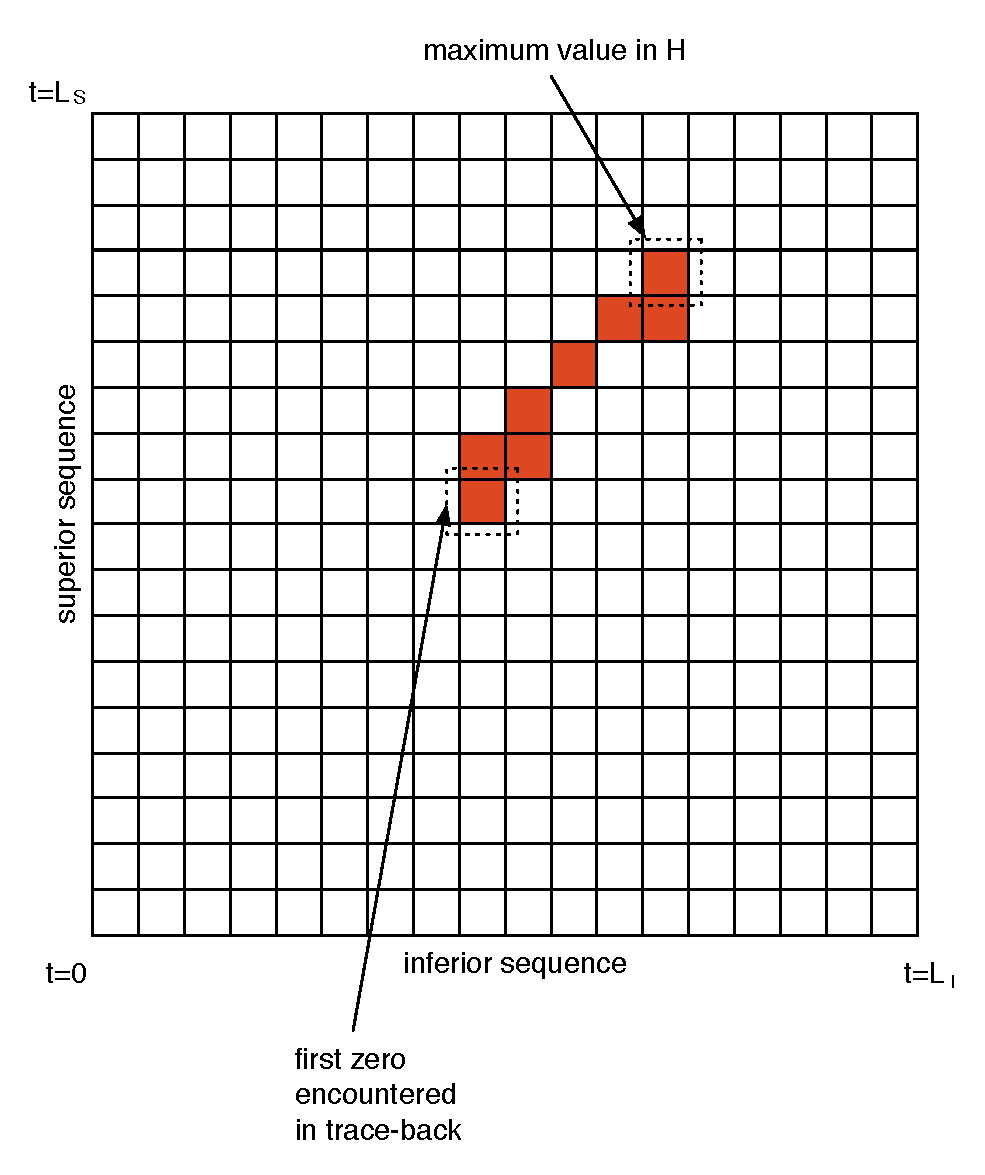
\includegraphics[scale=0.75]{SIC-DPLA_1}
\caption[Finding the optimal subsequence]{The optimal local alignment ends with the maximum value of H. Once it has been found, we trace backwards (either below, to the left, or diagonally down and to the left) along the path that generated the final alignment score until we find a $0$, which marks the beginning of the local alignment.}
\end{center}
\vspace{6pt}
\end{figure}

\item Calculate the aligned-Euclidean distance over all aligned vectors found in step 1 
\clearpage
and store this along with the length of the aligned vector sequences.
\end{enumerate}
DPLA and SW are only concerned with the best subsequence alignment between two sequences and so they would both be satisfied at the end of this step. We are also interested in this alignment, but we must continue to search for other subsequence alignments between what is left in our superior sequence (after removing the subsequence found in steps 1-2) and the entirety of our inferior sequence. Therefore, we continue on with the following:
\begin{enumerate}
\setcounter{enumi}{2}
\item Remove the submatrix from $H$ that corresponds to the superior sequence's optimally-aligned subsequence (found in step 1) (see Figure 48).
\begin{figure}[h!]
\vspace{24pt}
\begin{center}
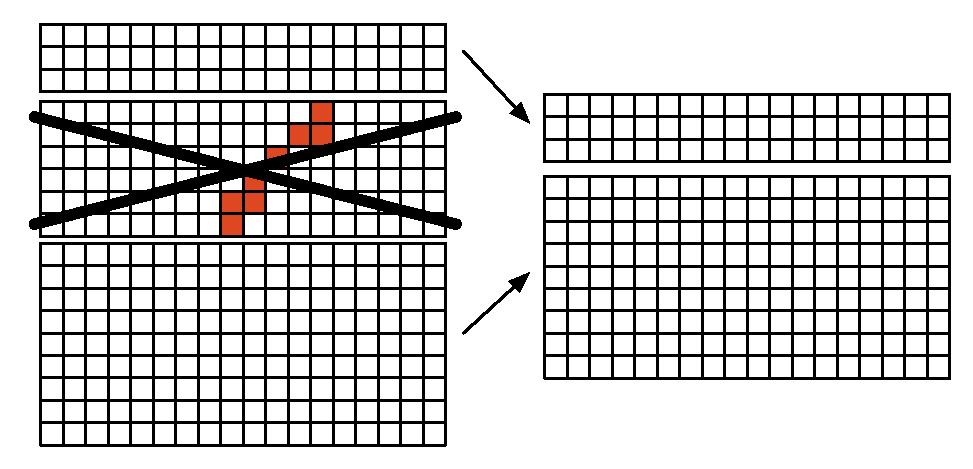
\includegraphics[scale=0.8]{SIC-DPLA_2}
\caption[Removing the optimal subsequence]{After the aligned-Euclidean distance is calculated for the optimal local alignment, the superior's subsequence involved in that alignment is removed.}
\end{center}
\end{figure}
\item Repeat steps $1-3$ until there are no longer any values in H above 0.
\item Calculate the sum of all distances generated in the various passes through step 2 and divide by the length of the superior sequence to normalize for sequence length.
\end{enumerate}

This process will give us a preliminary value for the IC-DPLA distance in one direction (e.g. where $Z^1$ is treated as the superior sequence and $Z^2$ the inferior):
\begin{equation}
D_{IC-DPLA_{S \to I}}^{(Prelim)} = \frac{\sum_{j=1}^J \sum_{k=1}^{K(j)} \sqrt{ \sum_{l=1}^L (A_{jkl}^1 - A_{jkl}^2)^2}}{L_S}
\end{equation}
where $D_{IC-DPLA_{S \to I}}^{(Prelim)} $is the preliminary IC-DPLA distance from superior sequence $S$ to inferior sequence $I$, $J$ is the number of subsequences chosen for alignment, $K(j)$ is the length of the $j$th subsequence pair, $L$ is the dimensionality of our timbre vector, $A_{jkl}^1$ is the $l$th element of the $k$th vector in the $j$th aligned subsequence taken from $S$, $A_{jkl}^2$ is the $l$th element in the $k$th vector in the $j$th aligned subsequence taken from $I$, and $L_S$ is the length of $S$.

Once we calculate our preliminary IC-DPLA distances in both directions, we penalize the alignment combinations chosen by scaling the preliminary distances in the following ways:
\begin{itemize}
\item If alignments are not ordered appropriately in time (i.e. if the aligned subsequences do not progress forward in time for both sequences) then the appropriate IC-DPLA distance is scaled by the the following swap penalty:
\begin{equation}
P_{SWAP} = \frac{N_S+N_T}{N_T}
\end{equation}
where the number of necessary subsequence swaps for the inferior sequence to match the progression of the superior sequence is $N_S$ and the total number of subsequences is $N_T$ (see Figure 49).
\begin{figure}[h!]
\begin{center}
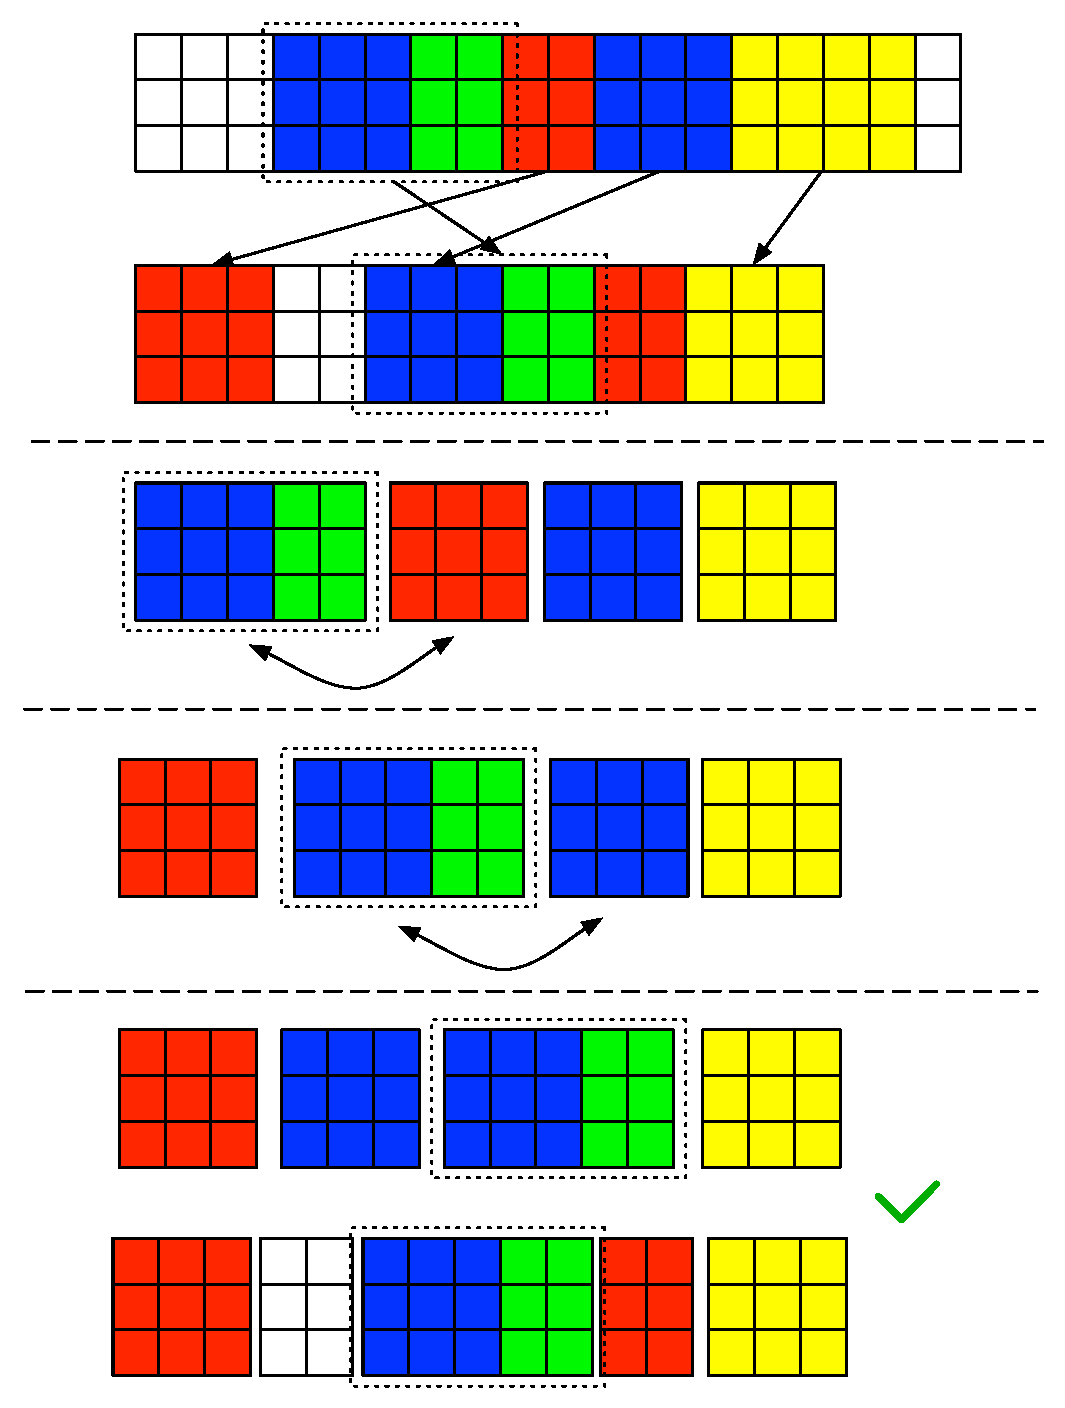
\includegraphics[scale=0.7]{Penalty_1}
\caption[Penalizing swaps]{Two swaps are necessary to return the progression of aligned subsequences from the inferior sequence back to its original ordering.}
\end{center}
\vspace{6pt}
\end{figure}
This value is at least one (when no swaps are necessary to appropriately align the sequences). 
\item There is an overlap/gap penalty enforced if the segments chosen from the inferior 
\clearpage sequence overlap one another and/or if there are any missing segments from the inferior sequence that are not present in the alignment with the superior sequence (see Figure 50). The penalized overlaps are those that result in less overlap when included than a gap if excluded. Otherwise, the overlap is flagged as a \textit{repetition} and dealt with separately (see next penalty item). Once repetitions have been removed, the cumulative overlap and cumulative gap amounts are summed over the length of the entire sequence, added to the inferior sequence length, and then the result is divided by the inferior sequence length to obtain the penalty amount. This value is used to further scale the distance and, like the swap penalty, is also at least one.
\begin{figure}[h!]
\begin{center}
\includegraphics[scale=0.7]{Penalty_2}
\caption[Penalizing overlaps and gaps]{The blue region is used twice by the superior sequence and is marked as a repetition, not to be penalized here. However, the two 2-vector gaps are penalized.}
\end{center}
\vspace{12pt}
\end{figure}
If $L_O$ is the cumulative overlap, $L_G$ is the cumulative gap, and $L_I$ is the total length of the inferior sequence, the penalty multiplier will be:
\begin{equation}
P_{O/G} = \frac{L_O+L_G+L_I}{L_I}
\end{equation}
\item If any repetitions are extracted from the previous overlap/gap distance adjustment, they also affect the distance measurement, but to a lesser degree than an overlap if the repetition is long, since an exact repetition of a lengthy subsequence should not penalize the similarity of timbral evolution to a large degree. We penalize the distance measure by counting the number of repetitions (and therefore disregarding their lengths), adding this to the number of total subsequences extracted, and the dividing the result by the number of subsequences extracted to give us a repetition adjustment scaling factor. If the number of repetitions is $N_R$, the penalty multiplier will be:
\begin{equation}
P_{REP} = \frac{N_R+N_T}{N_T}
\end{equation}
In the example in Figure 50 there is only one repetition of five total subsequences aligned, producing a $P_{REP}=(5+1)/5=6/5$.
\end{itemize}

The three penalty scaling factors outlined above are all used to adjust the preliminary IC-DPLA distances calculated in each direction (from sequence $Z^1$ to $Z^2$ and $Z^2$ to $Z^1$):
\begin{equation}
D_{IC-DPLA_{S \to I}} = D_{IC-DPLA_{S \to I}}^{(Prelim)} * P_{SWAP} * P_{O/G} * P_{REP}
\end{equation}

The two resultant IC-DPLA distances are then summed together to provide the SIC-DPLA distance ($D_{SIC-DPLA}$), which, as previously shown, is used to calculate our timbral sequence similarity measure, $S_T$.

Our approach is still greedy in that we optimize local alignments without regard to how it will affect our overall global scores (i.e. we optimize before applying our scaling factors), but we believe it to be a considerable upgrade over typical DTW and non-time warped aligned-Euclidean methods. A more systematic and less greedy measure is left for future work.

\vspace{12pt}\section{Refining Search Using State-of-the-Art Genetic Programming}
By expressing synthesis algorithms using the tree representation previously discussed, the search space can be viewed as a set of synthesis tree topologies, where each point in the space corresponds to a topology with a unique set of parameters and objects. This is the most common input representation found in GP literature, which allows us to leverage much of the research carried out in this field in order to produce an effective system.

The GP system that we have designed follows the typical GP blueprint at a high level. We will provide only a brief overview of the mechanisms involved in such a system and then will discuss where we have chosen to experiment and in what ways. A more detailed treatment of Genetic Programming can be found in John Koza's book \textit{Genetic Programming: On the Programming of Computers by Means of Natural Selection} \cite{Koza:1992gp}.

As mentioned in Chapter II - Prior Work, genetic programming is a parallel search technique. This means that instead of starting by looking in one location in space and moving along some search path from there, genetic programming starts looking in many places at once and allocates more resources to those regions that show promise. The search process loosely models biological evolution and so borrows a number of terms from that domain. The number of points one searches over in algorithm space at each iteration is defined as the current \textit{population}. One starts with an (often randomly generated) \textit{initial population}. The objective function that one wants to maximize over the search is referred to as the \textit{fitness function} and each successive iteration favors regions of space with higher fitness as it \textit{selects} individuals for the next \textit{generation} to either \textit{mutate} or effectively \textit{mate} in a  \textit{crossover} process where algorithms swap pieces of their code.

The primary deterrent to using any GA variant is that, in comparison to other search techniques, it is a very slow search process. Todd and Werner note that ``the main reason for this sometimes-glacial pace is that...evolution builds systems through the gradual accrual of beneficial bits and pieces, rather than through systematic design or rapid learning from the environment'' \cite[p. 5]{Todd:1998tg}. Another reason for GAs inefficiency is the fitness calculation bottleneck, as discussed by Riionheimo \cite[p.10]{Riionheimo:2003qo}. Typically most of the search time is spent calculating the fitness of each individual. If a fitness calculation is not needed (i.e. if there is a known mathematical relationship between the input parameter space and the output space) then the search would be sped up tremendously. However, in the problems GA variants are typically used for, analytical solutions are often not available.

Due to its inefficiency, GAs are often used only as a last resort in search problems. However, for problems that are not well understood or which are known to have complex multimodal fitness landscapes (e.g. Automatic Programming), they often provide the only solution. Much research has been carried out to find ways in which to increase the efficiency of search. Most often, these methods are aimed at restricting the search space using a set of heuristics that include both problem-domain dependent and independent knowledge. The problem-domain independent methods designed to restrict the search space and/or improve the search \textit{quality} of the GP system influence every part of its structural design. 

We apply the term heuristics both to architecture decisions as well as limitations imposed on the architecture because, as pointed out by Vanneschi, ``the art of choosing an appropriate representation and an appropriate set of operators is often a matter of experience and intuition'' and therefore all design choices are either based on personal or historical trial-and-error \cite[p. 6]{Vanneschi:2004le}.

A number of GP enhancements have already been described. For example, the GP/SA architecture used both by Alcazar and Sharman \cite{Alcazar:1996la} as well as Garcia \cite{Garcia:2002cq} is a way to improve the parameter search using simulated annealing, which is likely better suited for its fitness landscape. Also, incorporating higher-level modules into the function set along with low-level building blocks has been shown to make GP more powerful in various problems \cite{Koza:1997zr}. 

Another enhancement to the proposed system is the ability for basic function elements to handle vectors as a native data type. The inability to, for example multiply a stream of numbers by a scalar, is cited by Holladay and Robbins as a major deterrent to Automatic Programming systems that require such operations \cite[p. 1]{Holladay:2007ct}. If such simple operations on vectors are not possible, then the loop structures underlying their execution would have to be evolved separately.

When applying methods to restrict the search space, one must be careful not to restrict the space within a region that does \textit{not} include the optimal solution. A popular way to naturally restrict the search space (without the possibility of omitting the optimal solution) is to use strongly-typed GP (STGP), which enforces data type constraints, so that only syntactically correct structures are searched  \cite{Vanneschi:2004le, Harris:1997qf, Pachet:2007if}. Basic GP does not enforce such rules and so it is possible that topologies will be searched that are invalid. Enforcing data type constraints during search is a simple way to disregard such topologies and make the search much more efficient. An example of a syntactically-correct Max patch and a syntactically-incorrect Max patch are shown in Figure 51. As previously discussed, we impose STGP by adhering to Max's syntax when generating patches in Python.

\begin{figure}[h!]
\begin{center}
\vspace{24pt}
\includegraphics[scale=0.70]{SyntacticCorrectness}
\caption[Strongly-typed genetic programming]{A syntactically correct Max patch that would be included in a STGP search space and a syntactically incorrect one that would not be (due to the labeled disallowed connection).}
\end{center}
\vspace{6pt}
\end{figure}
One of the major problems that GP systems face, efficiency-wise, is code bloat. Bloat, as defined in da Silva's dissertation, is ``an excess code growth without a corresponding improvement in fitness'' \cite[p. 2]{Silva:2008le}. There are a number of theories as to why bloat occurs in GP systems, but da Silva notes that strong evidence supports that bloat is a side-effect of the search for higher fitness and consequently intricately linked to GP search \cite[p. 9]{Silva:2008le}. The issue is analogous to the over-fitting problem in machine learning. da Silva writes that ``programs tend to grow until they fit the fitness data perfectly'' \cite[p. 9]{Silva:2008le}.

Da Silva separates bloat control methods into four categories based on where in the search process control is applied: evaluation, selection, breeding, and survival \cite[p. 11]{Silva:2008le}. In evaluation methods, the desire for parsimony is directly incorporated into the fitness function. Selection methods apply rules that favor parsimonious solutions when selecting individuals for breeding. Breeding methods introduce genetic operators that are designed specifically to restrict code growth. Finally, survival methods only allow candidates from one generation to move on to the next if they meet certain size requirements \cite[p. 11-12]{Silva:2008le}. 

In da Silva's dissertation, he rigorously compares the most popular methods in each category using a number of test problems, differing in complexity, representation, and domain. Da Silva finds that a combination of dynamic maximum tree depth (DMTD) and dynamic resource-limited GP (dRLGP) outperformed all other methods consistently \cite[p. 86]{Silva:2008le}. 

DMTD is an extension of the static-depth limits (SMTDs) imposed by both Wehn \cite{Wehn:1998bh} and Garcia  \cite{Garcia:2002cq} in their research to restrict the size of the evolved synthesis topology and, more importantly from a user perspective, the parameter set. The difference between DMTD and SMTD, as the names imply, is that DMTD imposes a depth limit that changes throughout the search process. Specifically, DMTD works by first setting an initial depth limit when generating the first population. A new individual that breaks this limit will be replaced by its parent, unless it is the most fit individual so far in the run. In that case, the dynamic limit is adjusted to match the most fit individual's length and breeding continues with the new limit until another most-fit individual breaks it \cite[p. 17]{Silva:2008le}.

dRLGP is a variant of resource-limited GP (RLGP). In RLGP, a single resource limit is imposed on the entire GP population \cite[p. 21]{Silva:2008le}. Every topology node and parameter node in a population is considered a resource. The limiting of such \textit{resources} models the limiting of natural resources available to a given biological population, which is considered a main component of evolution \cite[p. 21]{Silva:2008le}. The process works as follows: offspring of a population are sorted by fitness, followed by their parents; programs in this list are given resources going from most fit to least fit; if an individual needs more resources than are available, it is passed over and not allowed into the next population. dRLGP adjusts the size of the resource limit (to that of what is used in the current population) if the mean population fitness is greater than the mean fitness of the best population in the run thus far \cite[p. 22]{Silva:2008le}. 

Imposing such limits will pressure the system into developing parsimonious solutions (which is good for synthesis algorithm controllability and efficiency) while severely restricting the search space (which makes the search process itself more efficient). A further benefit of using these limits to control code bloat as opposed to evaluation, selection, or breeding methods, is that they are parameterless and can be used with any selection method \cite[p. 97]{Silva:2008le}.

Another solution that is commonly used to improve the efficiency of the search (which also has added benefits related to the quality of the evolved algorithms) is called the \textit{Parallel and Distributed Genetic Programming (PADGP)} technique based on parallelizing the GP search process \cite[p. 13]{Vanneschi:2004le}. In PADGP, the search divides the initial population into a number of subpopulations that evolve independently, with frequent exchange of individuals between subpopulations \cite[p. 174]{Vanneschi:2004le}. The only communication between subpopulations occurs when the exchange of individuals is necessary. The ability to evolve subpopulations independently allows one to parallelize the search process, speeding up the search tremendously \cite[p. 173]{Vanneschi:2004le}. However, the true benefit of the island model is that it prevents another major problem of GP, premature convergence \cite[p. 15]{Vanneschi:2004le}.

Vanneschi writes that ``premature convergence, both from the view of the variety of the fitness values and of syntactic structures, is an experimental evidence in almost all the GP applications'' \cite[p. 15]{Vanneschi:2004le}. Convergence is ``used to describe the state of affairs when the population becomes largely homogenous, consisting largely of variations on a single style of solution'' \cite[p. 26]{Vanneschi:2004le}. When this happens prematurely, the system will output a sub-optimal solution. Crossover, one of the two basic genetic operators used in GP (along with Mutation) allows propagation of small blocks of code that were useful in previous populations (or, at the very least, part of useful algorithms) into future populations. While this is the main mechanism for code re-use during the GP search, it ``tends to encourage a uniformity in building solutions and can contribute to convergence problems'' \cite[p. 30]{Wehn:1998bh}. Vanneschi shows, via rigorous testing, that the PADGP is a natural way of maintaining diversity, and thus preventing premature convergence, inside GP populations \cite[p. 213]{Vanneschi:2004le}. He compares the effects of this model to a number of other methods designed specifically to limit premature convergence and finds that it works as well or better than these other methods \cite[p. 221]{Vanneschi:2004le}. He notes that, additionally, ``one advantage of multiple populations as means for maintaining diversity is that, in contrast to the clever methods above, diversity is maintained ``for free'', so to speak, without any particular algorithmic device beyond the simple communication among islands'' \cite[p. 213]{Vanneschi:2004le}. Vanneschi also suggests that using the island model has a better chance at finding global optima in multimodal landscapes due to the division of the space into a number of mini-parallel searches, as opposed to a singular parallel search over the entire space \cite[p. 192]{Vanneschi:2004le}. He writes that this has the effect of speeding up the search as well and that parallel GP would provide for a more efficient search even if implemented on a single processor \cite[p. 230]{Vanneschi:2004le}.

In order to further restrict the search space, one can also develop heuristics appropriate for the specific problem-domain. A common example is restricting the possible parameter values by discretizing a finite range, as suggested by Riionheimo \cite[p. 6]{Riionheimo:2003qo}. This process provides the possibility of omitting the optimal solution from search and so restriction on parameter values should not be too severe. Riionheimo suggests attempting to limit the range of parameters so that they are able to just cover all possible musical \textit{tones} and discretize with a resolution that is below the discrimination threshold \cite[p. 6]{Riionheimo:2003qo} However, determining such ranges and resolutions is a complex process. Martens and Marui found that, at least for vibrato flange and stereo chorus, the useful ranges of parameters were roughly the same \cite[p. 4]{Martens:2009lo}. However, a more detailed study by McDermott et al. show that, in general, \textit{useful} parameter ranges vary for different synthesis topologies and therefore must be found for each new topology one is presented with \cite[p. 5]{McDermott:2005xq}. Thus, it is important to err on the side of caution when specifying such limits. 

One can also place limits on the functions used in each run. However, in general, ``the function and terminal sets should be chosen so as to verify the requirements of closure and sufficiency'', so restricting the function set can be as dangerous as limiting parameter ranges \cite[p. 22]{Vanneschi:2004le}. 

A method used to improve the ability of GP to find optimal solutions that is directed at the fitness function definition is presented by McDermott et al. \cite{McDermott:2006ud}. By defining a set of \textit{increasingly discriminating fitness functions (IDFFs)} one is able to reward minor progress at each stage of the search in a way not possible using a statically defined fitness function \cite[p. 15]{McDermott:2006ud}. The basic idea is to reshape the fitness landscape throughout the search so that the optimal solution becomes more and more difficult to obtain as the search progresses. Early on in the search when individuals in the population perform poorly, the grading mechanism is more lenient and differences between extremely poor solutions and only slightly better solutions is magnified. As the mean fitness over the population increases, the fitness function can grow to become more and more difficult to satisfy. In effect, one is manually evolving the fitness function along with the population.

\vspace{12pt}\section{Summary}
This chapter explained our approach to improving the current state-of-the art meta-synthesis systems. 

We first outlined our decision to use standard Max signal-processing objects to create our primitive sets and discussed the nuances involved in implementing a GP system within the Max environment.

We covered in detail the design of our system's fitness function. We first explained how we came to decide upon an appropriate objective timbre space (and therefore a timbre feature representation) using instrument clustering performance as a benchmark. This was followed by our goals and motivations for designing a new timbral similarity metric, leading to an in-depth discussion of its design. We named this metric symmetric iterative continuous DPLA (SIC-DPLA).

We ended the chapter with a discussion of a number of specific recent advancements in GP research that we explore in this study with the intent of making our system more efficient and able to produce more parsimonious and effective solutions.

It is our belief that the approaches discussed in this chapter can combine to push synthesis topology evolution past a point of only being able to generate simple, \textit{toy-example} topologies. By utilizing a meta-synthesis software environment like Max (that was specifically designed to provide synthesis building blocks with the exact level of abstraction required by an efficient GP system) and an improved timbral sequence similarity metric, and by leveraging recent advancements in GP research regarding improved efficiency and code-bloat reduction, we expect our results to contribute greatly to this area of research.
\vspace*{\QuarterPage}
\chapter{EXPERIMENTAL DESIGN} % * suppresses heading numbers
There are many variations of population initialization strategies, operations (known as \textit{genetic operators}) used to \textit{evolve} algorithms from generation to generation, and  selection criteria for the algorithms that are subjected to these operations. Therefore, not only is it important to test the effectiveness of recent advancements in GP research pertaining to improving efficiency and reducing code-bloat (covered in the last chapter), but it is also necessary to determine which combinations of population initialization strategies, genetic operators, and selection mechanisms produce optimal solutions.

Additionally, the fitness function is problem-dependent and the quality of the solutions found using GP is completely reliant on how well it models the actual fitness of each algorithm with respect to the stated goal.

In order to produce an optimal GP system, one must test each of the above components. Our efforts in evolving Max patches have led us to explore all facets of GP in depth and we have found, as will be detailed in Chapter V - Results, that varying some meta-parameters have a large impact on solution quality, while others seem to have very little. 

Figure 52 shows a more detailed flow diagram of our GP system than that in Figure 21.
\begin{figure}[h!]
\begin{center}
\includegraphics[scale=0.5]{OverallGPSystem}
\caption[Flow diagram of overall GP system]{Flow diagram of our GP system with components labeled by the section numbers in which they are discussed.}
\end{center}
\vspace{6pt}
\end{figure}
As can be seen in Figure 52, there are several modules that make up our sound synthesis search system. Each module represents at least one variable of the system that contributes to its ability to find the optimal solution as quickly (i.e. within the smallest number of iterations) as possible. Given the high-dimensionality of this variable set, it is infeasible to perform an appropriate search over all of its various permutations within a reasonable amount of time. We instead take a measured approach to modifying one variable at a time while holding all others constant. Specifically, we first test those variables that we believe are least dependent on what the other variables are set to. Once we have optimized one variable, we move to the next least dependent variable and continue this way until we reach the most dependent. Using this approach, we will be able to test the highly dependent variables given a fixed set of near-optimal values/methods for all of the others, thereby decreasing the chance that any noticeable shortcomings of a chosen value/method for one variable are actually a result of the sub-optimal configuration of any other. In testing each variable, we use key metrics designed specifically for it.

With this methodology in mind, we have chosen to first examine our fitness function, as it will be required to measure the success of all of the various flavors of our system that we'll test.

\vspace{12pt}\section{Timbral Similarity Testing}
In order to test our SIC-DPLA similarity measure versus the three state-of-the-art approaches that motivated it (aligned-Euclidean, global DTW, and DPLA), we developed a controlled experiment that applies various kinds of temporal distortion to a given sound (at various levels of severity for each temporal distortion) and measures the similarity of each distorted copy with the undistorted original. The results of this experiment will highlight trends in how the tested similarity measures assign scores as each distortion is made more severe.

The distortions applied are broken into the following categories:
\begin{itemize}
\item Global time scaling (randomly selected between a $2-500\%$ increase in scale) combined with time shifting (randomly selected between $100-500ms$).
\item Random sample deletion (randomly selected and totaling between $2-75\%$ of all content).
\item Random extension of stable timbral content randomly selected and totaling between $2-500\%$ of all content. This can be seen as a way to apply time warping to a sound.
\item Introducing new timbral content (between $10-500\%$ of the file length) while randomly deleting other content.
\item Reordering random subsequences within content (by choosing subsequences that are between $10-20\%$ of the file length and swapping out of order up to $20$ times).
\item Randomly inserting repetitions paired with random deleting of non-repetitive segments (by choosing up to $10$ subsequences that are between $10-20\%$ of the file length and repeating each up to $10$ times).
\end{itemize}

Ideally, we want the amount of distortion severity to be inversely related to the similarity calculated. However, \textit{distortion severity} is a fuzzy concept and so for each distortion type, we substitute in its place the parameter that we believe to most align with it. For example, we measure distortion severity as the percent of content inserted (in relation to the original sound's length) in the case where we introduce new timbral content as a distortion.

The sounds we distort are the same sounds that we use as real-world targets in generalization testing, as discussed at the end of this chapter.

\vspace{12pt}\section{Genetic Operator Variations}
In order to implement a genetic algorithm within an automatic programming framework, one needs to develop an appropriate representation of each program, which we have done in Chapter III - Approach. This representation allows us to express all synthesis algorithms as a set of trees. However, this is not enough to define an input space. In order for a set to become a space, a topological ordering must be placed on the elements. This ordering will inform the shape of the objective landscape (i.e. fitness function) and consequently directly influence the difficulty of search through the space for some desired solution. In algorithm space, such orderings are typically not made explicit due to its complexity. Instead, implicit orderings are acquired via the operators used to search the space (da Silva, 2008, p. 102). Thus, using different operators will result in search spaces with different organizations. The goal is to find the input-space organization that makes the objective landscape as \textit{searchable} as possible. This can be measured via the negative slope coefficient (NSC), developed by \cite[p. 54]{Vanneschi:2004le}.

The NSC is computed by first generating a fitness cloud, where one plots the fitness of each individual by the fitness of one of its neighbors (children in GP parlance). The shape of this cloud provides some intuition of the evolvability of the genetic operators used and thus some intuition about the difficulty of the problem using these operators \cite[p. 130]{Vanneschi:2004le}. Vanneschi found that using uniform random sampling when generating individuals to use in the the fitness cloud typically results in individuals whose fitnesses tend towards the lower end of the fitness range. Therefore, this strategy does not give a complete picture of how fit neighbors are for individuals throughout the entire fitness spectrum \cite[p. 132]{Vanneschi:2004le}. Instead, Vanneschi suggests using the \textit{Metropolis-Hastings} sampling technique, which we have adopted in our work. An explanation of this technique with accompanying pseudo-code may be found on p. 131 of Vanneschi's PhD thesis \cite{Vanneschi:2004le}. The benefit of this sampling technique over uniform sampling is that it tends to produce a population whose fitness distribution is well approximated by a normal distribution. In other words, the resultant fitness clouds produced when using Metropolis-Hastings sampling do a better job at illustrating problem difficulty over the entire fitness range than those that utilize uniform random sampling.

Vanneschi also notes that choosing an appropriate neighbor from an individual (via the application of a genetic operator) is only useful if that neighbor would not be immediately discarded via the selection mechanism. Thus, Vanneschi suggests that neighbors are found via a Tournament Selection process (discussed in detail later in this chapter), where $k$ randomly generated neighbors enter a tournament and the winner is chosen as the neighbor to use in the fitness cloud. We have also adopted this strategy. Following Vanneschi's suggestion, we choose only one neighbor per individual, which is selected as the winner of a tournament of size $k=10$.

The NSC is calculated by partitioning the x-coordinate of the scatterplot into M segments of the same length and then dividing the y-coordinate into the ranges spanned by each x-segment. The average x and y values are calculated in those regions and a piecewise linear function is generated through those points. The slopes of the piecewise segments are calculated and only the negative values are summed to provide the NSC. 

In other words, for each segment $S_i$, the slope $P_i$ is calculated in the following way:
\begin{equation}
P_i = \frac{N_{i+1}-N_i}{M_{i+1}-M_i}
\end{equation}
where $M_i$ is the average of the original individual fitness values within the $i$th partition and $N_i$ is the average of the selected neighbor fitness values within the $i$th partition. The NSC is calculated from these slopes as:
\begin{equation}
NSC = \sum_{i=1}^{M-1} max(0, P_i)
\end{equation}
If $NSC = 0$, the problem is considered easy, if $NSC < 0$ it is difficult, and the value of NSC quantifies this difficulty (p. 139). In our experiments, we have chosen $M=10$ so that we can generate enough points per segment of the fitness cloud given a relatively small sample size of $1000$ for the average values to be descriptive of the segment.
The genetic operations we have decided to test are the most common set found in GP problems. A brief description of each follows:
\begin{description}
\item [Crossover] - In crossover, two trees are selected at random within the population, a subtree from each is selected and removed, and then the subtrees are attached to the cut points of the opposite trees. When ensuring syntactic correctness through the search process, the crossover operation must make sure to only choose subtrees that can be swapped and still result in syntactically correct structures (see Figure 53). 
\begin{figure}[h!]
\begin{center}
\vspace{24pt}
\includegraphics[scale=0.5]{Crossover}
\caption[Crossover]{Tree crossover with the root (i.e. dac\texttildelow{} below the terminals).}
\end{center}
\end{figure}
\clearpage
\\
\item[Subtree Mutation] - This, unlike crossover, is a unary operator, which removes a subtree at a random location within a tree and replaces it with a randomly generated subtree. As with crossover, syntactic rules must be enforced during generation of this new subtree (see Figure 54).
\begin{figure}[h!]
\vspace{24pt}
\begin{center}
\includegraphics[scale=0.5]{SubtreeMutation}
\caption[Subtree mutation]{Subtree mutation with the root (i.e. dac\texttildelow{} below the terminals).}
\end{center}
\end{figure}
\\
\item[Point or Node Replacement Mutation] - Instead of removing an entire subtree and replacing it with a randomly generated subtree, point mutation randomly removes a single node in a tree and replaces it with a node that is syntactically valid in that position (i.e. with the same number of inputs and the same input/output types) (see Figure 55).
\begin{figure}[h!]
\vspace{24pt}
\begin{center}
\includegraphics[scale=0.5]{PointMutation}
\caption[Point mutation]{Point mutation with the root (i.e. dac\texttildelow{} below the terminals).}
\end{center}
\vspace{6pt}
\end{figure}
\\
\item[Reproduction] - This is the simplest of all genetic operators in that it is simply a pass-through mechanism for selected patches. Reproduction allows for highly fit individuals to remain in the population from generation to generation so that they may be involved in crossover with other individuals (and so they can be continuously mutated) in the hope that a higher fit individual will result (see Figure 56).
\begin{figure}[h!]
\vspace{24pt}
\begin{center}
\includegraphics[scale=0.5]{Reproduction}
\caption[Reproduction]{Reproduction with the root (i.e. dac\texttildelow{} below the terminals).}
\end{center}
\end{figure}
\\
\end{description}

We have decided to use the following combinations of genetic operators (and proportions of how many patches undergo each operation in the combination) and have tested their ability to simplify the search problem using NSC:

\begin{itemize}
\item 75\% Crossover, 25\% Subtree Mutation
\item 75\% Crossover, 25\% Point Mutation
\item 25\% Crossover, 75\% Subtree Mutation
\item 50\% Crossover, 25\% Subtree Mutation, 25\% Point Mutation
\item 50\% Crossover, 25\% Subtree Mutation, 25\% Reproduction
\item 25\% Crossover, 50\% Subtree Mutation, 25\% Reproduction
\end{itemize}
As previously mentioned, each of these tests consist of generating $1000$ patches using the Metropolis-Hastings sampling technique and selecting one neighbor for each of these patches from the winner of a Tournament Selection process involving $10$ randomly generated neighbors in a manner consistent with the combinations listed above.

The targets used in this testing are the same as those used in generalization testing, as examined at the end of this chapter.

\vspace{12pt}\section{Target Sound Selection}

The previous discussion has provided a means to develop an appropriate fitness function for our problem and an input space that makes its corresponding fitness surface (given the pre-defined fitness function) as easily-searchable as possible within the GP framework. Going forward, we want to make sure that what we are testing is the appropriateness of our search technique over this space and corresponding fitness surface and not the appropriateness of or ability for sounds to actually be realized in Max. For example, there may be time-varying timbres that require tens of thousands of Max objects to replicate perfectly.

As Mitchell points out in his work on sound matching via evolutionary methods, the difficulties in obtaining an optimal solution to a complex search problem are based on several factors, only one of which is the search algorithm itself \cite[p. 1]{Mitchell:2007fe}. He recommends using a \textit{contrived} target in order to test only the efficacy of the search. In our problem domain, a contrived target refers to one that was generated by a known synthesizer (i.e. a Max patch). Mitchell suggests randomly generating contrived targets using points uniformly spread out in the input-space \cite[p. 2]{Mitchell:2007fe}. If the search algorithm is able to match all of the contrived targets with a good spread in the input space, it is suggested that one can then assume it will be able to match any target \cite[p. 2]{Mitchell:2007fe}. This assumes however that a uniformly spread set of points in the input space will map to a large area of the timbre space, which is not necessarily the case.

We therefore have chosen to test the search algorithm on three contrived targets with varying degrees of temporal complexity and dissimilar timbral content in order to attain an understanding of the limitations of the search algorithm (see Figures 57, 59, and 61). 

In Figure 57, we present a Max patch that processes a sine wave through a feedback delay unit and modulates the result with a frequency-varying sine wave LFO, which produces a smooth and quick pulsation effect.
\begin{figure}[h!]
\vspace{24pt}
\begin{center}
\includegraphics[scale=0.8]{DelayFeedbackAM}
\caption[Delay feedback AM Max patch]{A Max patch that generates audio by downsampling a $300$ Hz sine wave, passing it through a $500$ ms feedback delay line with feedback varied by a $10$ Hz sine wave, and then amplitude modulating it with a $20$ Hz frequency-modulated sine-wave LFO.}
\end{center}
\vspace{6pt}
\end{figure}
We refer to this patch as the feedback-delay-AM target going forward. Figure 58 provides a time-frequency representation of the audio this patch produces:
\begin{figure}[h!]
\vspace{30pt}
\begin{center}
\includegraphics[width=\linewidth]{FeedbackDelayAMTargetSTFT}
\caption[Delay feedback AM time-frequency representation]{A time-frequency representation of the audio produced by the Feedback-Delay-AM target patch.}
\end{center}
\vspace{6pt}
\end{figure}

In Figure 59, we present a Max patch that down samples an 8-bit sine wave by an amount proportional to the amplitude of a sine wave modulated by a sawtooth. 
\begin{figure}[h!]
\begin{center}
\includegraphics[scale=0.8]{AdaptiveDegrade}
\caption[Adaptive downsampling Max patch]{A Max patch that generates audio by downsampling a $400$ Hz, $8$-bit sine wave by an amount that is proportional to the amplitude of an amplitude modulated $200 Hz$ sine wave by a $1$ Hz sawtooth modulator.}
\end{center}
\vspace{6pt}
\end{figure}
The result sounds like a harsh bandpass filter sweeping over an abrupt impulse with a constant drone in the background. We refer to this patch as the adaptive-downsampling target going forward. Figure 60 provides a time-frequency representation of the audio this patch produces:
\begin{figure}[h!]
\begin{center}
\includegraphics[width=\linewidth]{AdaptiveDownsamplingTargetSTFT}
\caption[Adaptive downsampling time-frequency representation]{A time-frequency representation of the audio produced by the Adaptive-Downsampling target patch.}
\end{center}
\vspace{6pt}
\end{figure}

Figure 61 shows a Max patch that regularly clips, but within those hard clips exists a reverberant sound similar to waves crashing in succession. 
\begin{figure}[h!]
\begin{center}
\includegraphics[scale=0.8]{ClippingReverbSaw}
\caption[Clipping reverb sawtooth Max patch]{A Max patch that generates audio by adding a $50$ Hz sawtooth wave with a sawtooth wave passed through a reverberator with a $3$ s reverb time whose frequency is varied by another reverberated sawtooth wave with a reverb time of $500$ ms and a frequency of $5$ Hz.}
\end{center}
\vspace{6pt}
\end{figure}
We refer to this patch as the clipping-reverb target going forward. Figure 62 provides a time-frequency representation of the audio this patch produces.

Since these contrived targets are realizable in the Max environment, they should be found given an intelligent enough search. While it is important that these targets are sufficiently spread out in the input space in order to promote some sense of generalization of the search technique through this space, we later test the search technique using non-contrived targets in order to provide a more resounding argument for this.

We are able to measure success in two different ways when using contrived targets and will speak to both in the results section whenever our tests involve them:
\begin{enumerate}
\item We are able to compare the topographies of the contrived-target patch and the best-of-run patch that is generated during the search process. If the topographies are exact matches, we must consider this an outright success. However, if different, the topologies provide intuition about how code bloat enters the search, how well the topologies of local optima mirror the target topology (i.e. if there is a correlation between timbre and topology space), and how well different topologies can mimic the timbre produced by a contrived-target topology (i.e. how realizable is the target timbre given topologies that differ from the topology that generated the target).
\item We are able to measure the best-of-run fitness and determine how well our search is able to achieve its goal of finding a patch that can produce the target timbre.
\end{enumerate}

It should be emphasized that during the tests involving contrived targets, the function/object sets provided to the algorithm will contain only the necessary objects and will enforce tight parameter restrictions on each object in order to give the algorithm the best chance at reaching them. We later look at how the quality of our best-of-run patches and the speed at which we find them changes as we restrict and expand our function sets and parameter ranges.
\clearpage
\begin{figure}[h!]
\begin{center}
\includegraphics[scale=0.35,width=\linewidth]{ClippingReverbTargetSTFT}
\caption[Clipping reverb sawtooth time-frequency representation]{A time-frequency representation of the audio produced by the Clipping-Reverb target patch.}
\end{center}
\end{figure}

\section{Limiting Code Bloat and Promoting Parsimony}
By using contrived targets and objects that are able to construct them perfectly, we have set up a self-fulfilling prophecy of sorts that would rarely be encountered in practice. It is important to look at how our solutions degrade (or to what degree the time it takes to find an optimal solution increases) once the object set grows beyond the necessary set of objects and/or necessary objects are removed from the object set. However, before these parameters are varied, we look at other sorts of resource limitations that have proven effective in other GP research to see if they are useful in this problem space. We are able to focus on the efficacy of these methods and provide appropriate comparisons if we tightly control our experiments in the way previously suggested.

In Chapter III - Approach, we listed a number of methods for limiting the region of input space we will search over including: enforcing strong typing constraints, applying either static (SMTD) or dynamic maximum tree depths (DMTD), and/or enforcing limitations on the total amount of resources in a given population using either resource limited GP (RLGP) or dynamic resource limited GP (dRLGP) constraints. These methods were developed to be used for any problem domain and only discriminate against solutions that are not parsimonious or syntactically valid. They promote efficiency and low storage requirements as well as controllability of the resulting algorithms due to their propensity to generate low-dimensional parameter sets. However, as with any kind of limitation of the searchable input space, we must make sure not to exclude possible solutions. Therefore, a fine balance must be found between the improvements in the efficiency of the search (i.e. iteration count to the optimal solution) and the decrease in fitness of the optimal solution found. Since we can be sure that all solutions are attainable for our contrived targets and associated object sets, we can fairly compare different severities of limitation across all targets.

A brief recount of each limitation follows:
\begin{description}
\item [Static Maximum Tree Depth (SMTD)] - Throughout the entire search process, a static limit is placed on the maximum tree depth of each individual.
\item [Dynamic Maximum Tree Depth (DMTD)] - DMTD works by first setting an initial depth limit when generating the first population. A new individual that breaks this limit will be replaced by its parent, unless it is the most fit individual so far in the run. In this case, the new most-fit individual's depth is used as the limit going forward.
\item [Resource Limited GP (RLGP)] - Throughout the entire search process, a static limit is placed on the number of resources (i.e. the sum of function and terminal nodes) used in an entire population. This limit is therefore applied to the overall population as opposed to SMTD and DMTD, which is applied to each individual in a population.
\item [Dynamic Resource Limited GP (dRLGP)] - Throughout the search process, the limit placed on the amount of resources available to a population increases if the mean population fitness of a specific generation (before the limit is applied) is greater than the mean fitness of the best generation up to that point in the run. 
\end{description}

To test the effects of these limitations, we use the contrived target set, apply these limitations at various severities, and calculate how the fitness of the optimal solutions are affected as a function of limitation severity. 

Since, at this point in our experimentation, we will not have tested either how best to initialize our population or how we should select individuals to undergo genetic operations to produce each successive generation, we choose to use the most commonly utilized methods during these tests: grow initialization and fitness-proportionate selection (see Section 3.2.5). We intend to improve upon these (if improvements are possible) in separate testing after we've determined the best mechanism for promoting parsimony. 

We are interested in recording the fitness of the best-of-run individual over a set number of iterations for every permutation of the aforementioned code-bloat reduction mechanisms. In our testing, we run experiments while imposing each of the following search space limitation constraints over $200$ iterations of $100$ individuals, for each of the contrived targets:
\begin{itemize}
\item A SMTD of $4,6,8, 10, 12 \text{ and }14$.
\item A DMTD starting at $6$ with a hard limit at $10$, one starting at $8$ with a hard limit at $12$, and one starting at $10$ with a hard limit at $14$.
\item A RLGP of $1000, 1500, 2000, 2500, \text{and } 3000$.
\item A dRLGP starting at $1000$ with a hard limit at $2000$, one starting at $1500$ with a hard limit at $2500$, one and starting at $2000$ with a hard limit at $3000$.
\item A SMTD of $6$ and a RLGP of $1500$ as well as a SMTD of $10$ and a RLGP of $2500$.
\item A DMTD starting at $6$ with a hard limit at $8$ and a dRLGP starting at $1500$ with a hard limit at $2500$ as well as a DMTD of $6$ with a hard limit at $14$ and a dRLGP starting at  $1000$ with a hard limit at $3000$.
\end{itemize}

\vspace{12pt}\section{Initial Conditions and Selection Methods}

Along with algorithm representation and operator selection, the population initialization and selection mechanisms form the basis of the GP architecture. It may seem strange to first look at limiting code bloat and promoting parsimony before exploring these fundamental GP mechanisms. We have chosen this ordering because of the benefits reducing code bloat and promoting parsimony provides to all testing that follows it. Testing of the remaining parts of our system requires full test runs. By applying the mechanisms explored in the previous section, these test runs will be able to run more efficiently by not looking in regions of the input space that we are not interested in (i.e. those that would produce syntactically invalid Max patches or those whose solutions would be complex and likely unable to run in Max in real time). This benefits the testing of all other parts of the GP system, because it allows test runs to achieve better fitness earlier on so that one can discriminate between, for example, initialization methods over higher elevations in the fitness landscape (i.e. closer to the optimal solution), which is where the impact of choosing one variation over another is most significant.

The three initialization flavors we study are full, grow, and ramped half-and-half initialization. A brief description of each of these methods follows:
\begin{description}
\item [Full Initialization] - The root node is chosen and then, in a depth-first fashion, function nodes are added until the maximum tree depth is reached, at which time a terminal node is chosen. This process is repeated for all branches, resulting in a full tree where each branch meets the maximum tree depth. The risk of using full initialization is that one may start with a population where individuals are too similar (given that they are all full tree structures).
\item [Grow Initialization] - This is very similar to full initialization, except that as the branches are being built, each node is selected from the pool of both function and terminal nodes. The result is a tree with branches that are no greater than the maximum tree depth, but that may be shorter (due to a terminal node being chosen before the maximum depth is reached). The risk of using grow initialization is that it may result in a population with too many individuals whose branches have terminated prematurely and are therefore too simple to perform any meaningful function.
\item [Ramped Half-and-Half Initialization] - This uses full initialization for half of the individuals in the population and grow initialization for the other half. It also increases the depth limit for both methods as the population grows in size. The ramping of the depth limit along with using both full and grow methods produces a wide variety of patches in shape and size.
\end{description}

The four selection methods we have chosen are known as Fitness-Proportionate, Ranking, Tournament, and Double Tournament. A brief description of each of these methods follows:
\begin{description}
\item [Fitness-Proportionate Selection] - Individuals from one generation are chosen to populate the next generation with probability proportional to their fitness. Thus, the more fit an individual is, the more likely it will be chosen to breed new individuals for the next generation. In Figure 63, the top row of squares represent the individuals in a population and the pie chart below represents their respective fitnesses as fractions of the sum of all fitnesses in the population. 
\begin{figure}[h!]
\vspace{24pt}
\begin{center}
\includegraphics[scale = 0.7]{PieChartSelection}
\caption[Fitness-proportionate selection]{In fitness-proportionate selection, individuals are assigned selection probabilities proportional to their fitness score.}
\end{center}
\vspace{6pt}
\end{figure}
In other words, for fitness-proportionate selection, the pie chart illustrates the probability with which each individual will be selected to breed the next population. Note in the figure that the red and green individuals from this example are chosen twice due to their high fitnesses (i.e. probabilities of selection), while the yellow is not chosen due to its low fitness.

\item [Ranking Selection] - In ranking selection, individuals from one generation are ranked in order from least to most fit and the probability of selection is proportional to this ranking (see Figure 64). 
\begin{figure}[h!]
\begin{center}
\includegraphics[scale = 0.6]{RankSelection}
\caption[Ranking selection]{In ranking selection, individuals are assigned selection probabilities proportional to their fitness rank from lowest-to-highest fitness.}
\end{center}
\vspace{6pt}
\end{figure}
For example, if there are $N$ individuals in a generation, then the least fit individual has rank $1$ and the most fit rank $N$. The sum of all ranks is $N(N+1)/2$. Therefore, the least fit individual will have a selection probability of $1/(N(N+1)/2)$ or $2/(N(N+1))$ regardless of its fitness value and the most fit individual will have a selection probability of $N/(N(N+1)/2)$ or $2/(N+1)$ regardless of its fitness value. 

\item [Tournament Selection] - In tournament selection, a set of patches are selected at random from a generation and the most fit of those patches is selected. The previously chosen set of patches are placed back in the pool of all patches to be randomly sampled from on the next iteration (see Figure 65). 
\begin{figure}[h!]
\begin{center}
\includegraphics[scale = 0.6]{TournamentSelection}
\caption[Tournament selection]{In tournament selection, individuals are randomly chosen to vie for a selection spot in the tournament. Once a winner is decided and selected, all participants are put back into the pool before another random group is chosen for competition.}
\end{center}
\vspace{6pt}
\end{figure}
This random sampling of patches and the tournament that follows is repeated as many times as there are individuals to be selected.

\item [Double Tournament Selection] - In double tournament selection, each individual chosen to be part of the final tournament is already the winner of a tournament with different conditions. The most common double tournament Selection mechanism works by first choosing a random grouping of patches, selecting the most parsimonious of those patches with probability $D$, and placing the winner in a pool of other parsimony tournament winners to be involved in a fitness tournament (see Figure 66).
\\
\vspace{12pt}
\begin{figure}[h!]
\begin{center}
\includegraphics[scale = 0.7]{DoubleTournamentSelection}
\caption[Double tournament selection]{In double tournament selection, a few randomly chosen groups of individuals enter separate tournaments, with members of each group vying for a spot in a second tournament. The winner of this second tournament is selected to reproduce. Once a winner is decided and selected, all participants are put back into the pool before other groups are randomly chosen for competition.}
\end{center}
\vspace{6pt}
\end{figure}

The idea is that double tournament selection applies parsimony pressure absent from typical tournament Selection, which is useful for controlling code bloat. The most common tournament size for the parsimony tournament is two with $D = 0.7$. The most common tournament size for the fitness tournament is seven \cite[p. 21]{luke2006comparison}.
\end{description}

We have chosen to enumerate the various combinations of initialization and selection mechanisms in our tests as it is unclear exactly how correlated these two mechanisms are in producing an optimal search algorithm. We are interested in recording the fitness of the best-of-run individual over a set number of iterations for every combination examined. Again, our tests will involve moving through $200$ iterations of $100$ individuals. The combinations we test are listed below:
\begin{itemize}
\item full initialization and fitness-proportionate selection.
\item full initialization and ranking selection.
\item full Initialization and tournament selection.
\item full Initialization and double tournament selection.
\item grow initialization and fitness-proportionate selection.
\item grow initialization and ranking selection.
\item grow initialization and tournament selection.
\item grow initialization and double tournament selection.
\item ramped half-and-half initialization and fitness-proportionate selection.
\item ramped half-and-half initialization and ranking selection.
\item ramped half-and-half initialization and tournament selection.
\item ramped half-and-half initialization and double tournament selection.
\end{itemize}
The best combination of initialization mechanism and selection method, along with the choices  that will have already been made regarding the fitness function and code-bloat reduction approach, will provide us with an optimal base GP architecture. The following tests seek to augment this architecture and provide further evidence that it will generalize well to all timbres.

\vspace{12pt}
\subsection{Non-Standard Selection Methods}

Aside from the standard methods of patch selection, we mentioned (in Chapter III - Approach)  three other non-standard mechanisms that may be involved in the selection process that have shown to be useful for certain GP problems:

\begin{enumerate}
\item Using the parallel and distributed genetic programming (PADGP) paradigm, where subpopulations within the GP population are formed and individuals between populations are rarely allowed to interact, resulting in entire subpopulations that are allowed to evolve independently. The parameters to this model are the communication topology between subpopulations (i.e. who transfers individuals to whom), the number of subpopulations, the number of individuals per subpopulation, the frequency of exchange of individuals, and the number of individuals exchanged \cite[p. 178]{Vanneschi:2004le}. The three communication topologies used in the literature are the ring topology (where the subpopulations form a circle and each passes individuals in a clockwise manner), the grid topology, (where subpopulations form a grid and each population sends and receives individuals from all four neighbors), and the random topology (where each subpopulation sends individuals and receives individuals from exactly one random subpopulation different from itself at each migration period).
\item Applying Simulated Annealing (SA) on the parameter set of each patch in a population to find the optimal parameter set for the given patch topology before running the patches through the selection process.
\item Starting with a more lenient fitness function that the selection mechanism is aware of and making it more demanding over the lifecycle of the search, such that only in the last few iterations is the appropriate fitness measure applied before selection. The set of fitness functions involved are formally referred to as Increasingly Discriminating Fitness functions (IDFFs). 
\end{enumerate}

We believe our treatment of this problem would not be complete if we did not ascertain whether these more modern GP mechanisms could be helpful to us. The above approaches attempt to provide a more efficient means to achieve an optimal solution and we therefore test them on this ability. We are interested in recording the fitness of the best-of-run individual over a set number of iterations for every combination examined. In the case of using SA in combination with GP, it is not immediately clear how to directly compare this strategy with standard GP, due to the internal iterations SA proceeds through within each GP iteration. In this case, the number of algorithms searched (i.e. translated into the Max environment for audio processing) will be used for a fair comparison.

In our testing involving PADGP, we follow Venneschi's suggestion to use a random communication topology, a frequency of exchange of every ten generations, and a population exchange size of $10\%$ of the total number of individuals in each subpopulation \cite[p. 190]{Vanneschi:2004le}. We test this method using $200$ iterations of $100$ individuals, where the $100$ individuals are split into $5$ groups of $20$.

In testing Simulated Annealing on the parameter set of each individual between generations, we limit the system to search through as many individuals as we have in a typical run (i.e. $20,000$). If we allow each patch to undergo $10$ SA iterations, this reduces the number of iterations of GP to $20$. We do not want to limit the ability of our system to utilize GP and we feel that $20$ is possibly just enough iterations to leverage it, so we keep the SA iteration count at $10$. 

SA is a simple strategy that generates a random neighbor, calculates its fitness and a corresponding \textit{acceptance probability} (based on that fitness and the fitness of the current individual), compares the probability to a uniformly randomly chosen number, and makes the neighbor the new individual to run SA on if the probability is greater than the random number chosen. As the iteration count increases, the acceptance probability becomes more and more strict for poorly performing individuals. As is standard, we will use the Metropolis-Hastings algorithm to choose neighbors (where a neighbor in this context is a patch with the same exact topology, but where a single parameter is changed by no more than $50\%$ of its magnitude) and will assume an acceptance probability of:
\begin{equation}
P(S_{T_{p_1}}, S_{T_{p_2}}, T) = \left\{
   \begin{array}{l l}
    1 & \quad \text{if $S_{T_{p_2}}>S_{T_{p_1}}$}\\
    e^{-(S_{T_{p_2}} - S_{T_{p_1}})/T} & \quad \text{if $S_{T_{p_2}}\leq S_{T_{p_1}}$}
    \end{array} \right.
\end{equation}
where $S_{T_{p_1}}$ and $S_{T_{p_2}}$ are the similarity scores for some patches $p_1$ and $p_2$, and $T$ is the \textit{temperature value}, which will range from $1-10$ over the ten iterations (Kirkpatrick, Gelatt, and Vecchi, 1983, p. 673).

We also test the use of Increasingly Discriminating Fitness functions (IDFFs) as the system iterates through its search process. We choose to alter our discrimination by following the strategy used by McDermott et al. utilizing a \textit{layered learning} approach \cite[p. 3]{McDermott:2006jd}. In searching for an optimized parameter set for a given synthesis algorithm, McDermott et al. write that layered learning ``is motivated by the natural bottom-up decomposition of this type of problem into learning sub-tasks, and by the fact that evolutionary learning is not tractable when attempting to solve the entire hierarchy of sub-tasks simultaneously.'' The idea beyond layered learning is to first assign high fitness to individuals that exhibit pieces or building blocks of the desired output, so that they will live on in future generations when the fitness discrimination becomes more strict. If such building blocks are allowed to live on, they will be able to contribute to more advanced individuals that able to combine several different building blocks---deemed fit in early generations---to produce individuals that are deemed fit given higher standards.

We test this strategy by initially measuring how well individuals from early generations match partial subsequences of the final target timbral sequence. As the generation number increases, the fitness function incorporates more and more of the total target subsequence in its calculation, with hopes that fit individuals from early generations (that are well-suited to subsequences of the target) will combine in later generations to produce longer and longer matching subsequences, and finally the entire target sequence by the last generation.

\vspace{12pt}\section{Expanding/Restricting the Searchable Region of Input Space}
Once we have solidified the GP system, we can move away from using perfectly contrived examples in our experiments and towards \textit{real-world} use cases. This involves two steps:

\begin{enumerate}
\item We will both expand and contract the object and parameter sets used to generate Max patches when searching for our contrived targets. By looking at how well our solutions approach the contrived Max patches, we will be able to show how robust our system is when starting with an inappropriate resource set (e.g. one with objects that are not involved in the optimal solution and/or with necessary objects in the optimal solution not present). If the system is given a timbre that was produced (or is easily producible) by a Max patch, it is unlikely the object set we choose for our system to source from will contain all of the objects (and only the objects) necessary to build the target. Therefore, understanding the system's robustness with respect to object and parameter set expansion and restriction is important.

However, since a \textit{real-world} timbre may not even be realizable with 100\% percent accuracy in the Max environment, testing robustness in this way is not enough to show how well our system generalizes to all timbres. That being said, they are a good first step towards that goal and provide us with information regarding how well our system can perform when the target timbre can be realized within our environment.
\item The final step towards showing system generalization over all timbres involves using timbres that are not contrived. This is discussed in the next section.
\end{enumerate}

In the first set of use cases, we look at how well our best-of-run fitness is affected by using object and parameter sets that are either not sufficient or over-complete. For example, the feedback-delay-AM target requires an object set that includes: cycle\texttildelow{} (with a frequency range between $0-400$), degrade\texttildelow{} (with a downsample range between $0.4 - 0.6$ and no ability to reduce the bit-depth), *\texttildelow{}, \textit{loadmess}, and a feedback delay unit with a $500$ ms delay. We reduce this function set by removing degrade\texttildelow{} and disallowing a variable feedback amount to the delay. We expand the function set by adding objects that are not in the target, including a saw\texttildelow{} object, a /\texttildelow{} object, a +\texttildelow{} object, and a delta\texttildelow{} object and increase the parameter ranges to allow the cycle\texttildelow{}  to take on more typical values between $0-5000$ Hz and to allow degrade\texttildelow{}  to take downsample values between $0.1-0.9$ (where 1.0 means no downsampling) and to accept bit-depth changes so as to quantize its input into a $2$-bit, $4$-bit, $8$-bit, or $16$-bit signal. 

\vspace{12pt}\section{Generalization}
It is necessary to test this system on a number of real-world sounds in order to gauge its ability to generalize to sounds that are not contrived. As Riionheimo notes, ``the quality of re-synthesis of real recordings is more difficult to measure as there are no known correct parameter values'' nor synthesis topologies \cite[p. 13]{Riionheimo:2003qo}. In genetic programming research where a known target algorithm does not exist, the performance of the system is usually measured using the fitness level at which the system converges and how long it takes to converge to that level. We do not have a known topology for such real-world examples and therefore only use this measure to determine how successful our search method is. In order to determine how well our search generalizes over all real-world sounds, we have chosen five different target sounds ranging from those generated by music instruments to those generated in nature. We focus on both musical and non-musical sounds in order to test how well the system works when given some targets that are similar and some that are very different from the audio our underlying timbre feature space (used to generate the vector sequences we calculate timbral similarity over) was trained on. Targets were also chosen to contain both slowly varying and fast, repetitive timbral material in order to determine the ability of our system to generalize well for sequences that evolve at different time scales.

A brief description of the timbre targets we have chosen follows:
\begin{description}
\item[Evolving Lion Roar] - This is the sound of a lion roaring from start to finish with timbre evolving as the lion opens and closes his mouth. Figure 67 shows a time-frequency representation of this audio.
\begin{figure}[h!]
\begin{center}
\includegraphics[scale=0.34]{EvolvingLionRoarTargetSTFT}
\caption[Evolving lion roar time-frequency representation]{A time-frequency representation of the evolving lion roar target.}
\end{center}
\vspace{24pt}
\end{figure}
\item[Evolving Freight Train] - This is the sound of a freight train passing close-miked tracks, with an increasing amount of high pitched random screeching as the sound progresses. Figure 68 shows a time-frequency representation of this audio.
\begin{figure}[h!]
\begin{center}
\includegraphics[scale=0.34]{FreightTrainTargetSTFT}
\caption[Evolving freight train time-frequency representation]{A time-frequency representation of the Evolving Freight Train target.}
\end{center}
\end{figure}
\item[Evolving Metal Gong] - This is a single gong hit that evolves naturally with higher harmonics dying off before lower harmonics do. Figure 69 shows a time-frequency representation of this audio.
\begin{figure}[h!]
\begin{center}
\includegraphics[scale=0.34]{MetalGongTargetSTFT}
\caption[Evolving metal gong time-frequency representation]{A time-frequency representation of the Evolving Metal Gong target.}
\end{center}
\vspace{24pt}
\end{figure}
\begin{figure}[h!]
\begin{center}
\includegraphics[scale=0.34]{EvolvingMetallicSynthTargetSTFT}
\caption[Evolving metallic synth time-frequency representation]{A time-frequency representation of the Evolving Metallic Synth target.}
\end{center}
\end{figure}
\item[Evolving Metallic Synth] - This sound was generated by a software synthesizer inside Ableton Live and evolves in a complex manner. Figure 70 shows a time-frequency representation of this audio.
\item[Random Analog LFO Reverb] - This sound was generated by a software synthesizer inside Ableton Live that is modulated with a random LFO and put through a reverb plugin. Figure 71 shows a time-frequency representation of this audio.
\end{description}
\begin{figure}[h!]
\vspace{12pt}
\begin{center}
\includegraphics[scale=0.34]{RandomAnalogReverbTargetSTFT}
\caption[Random analog LFO reverb time-frequency representation]{A time-frequency representation of the Random Analog LFO Reverb target.}
\end{center}
\end{figure}
We have searched for these timbres using the optimal parameters/methods obtained in the previous tests, and extending our iteration count stopping criteria from $200$ iterations to $800$ to increase the likelihood of convergence over the run. We look at best-of-run fitness values for each individual real-world target used in our tests. The results of these tests can be found at the end of Chapter V - Results with an accompanying discussion.

%\vspace*{\QuarterPage}
\chapter{RESULTS} % * suppresses heading numbers	
\section{Finding an Optimal Similarity Measure for Time-Varying Timbre}
One of the most important parameters in any genetic algorithm (and thus any application of GP) is an appropriate measure of fitness. For our problem domain, we have developed the SIC-DPLA measure - over a sequence of feature vectors from a NLSE timbre space - in hopes to best represent our objective of matching timbral sequence similarity between two given sounds. In order to determine its efficacy, we have tested it against aligned-Euclidean, DTW, and DPLA measures in an experiment that determines the similarity between an undistorted sound and a large number of temporally distorted counterparts (as described in Chapter IV - Experimental Design). Each type of distortion was tested with $1000$ different randomly chosen parameterizations.

The results of this testing follows, with each plot showing the \textit{mean} normalized similarity scores under each distortion test case, calculated over individual scores from the $5$ real-world target files chosen for the generalization testing. The similarity scores for each similarity type were normalized over their natural range so as to better compare the effects that increasing distortion severity has on each type.

\subsection{Global Time Scaling}
The global time scaling distortion that we applied takes the feature data from the undistorted audio and stretches it by a randomly selected amount in a range between $2-500\%$ of the length of the undistorted feature data. Figure 72 shows the similarity scores assigned to over $1000$ randomly chosen stretch amounts.
\vspace{12pt}
\begin{figure}[h!]
\vspace{24pt}\begin{center}
\includegraphics[scale=0.5,width=\linewidth]{GlobalTimeScaling}
\caption[Global time scaling results]{Similarity scores under various amounts of global time scaling distortion.}
\end{center}
\vspace{6pt}
\end{figure}
All similarity measures trend downward (as desired) as the global scale percentage is increased, except for the DTW measure. Given that DTW should find its optimal path to be along the main diagonal, the fact that the score does not change significantly is expected. We view this as drawback of DTW, since our ideal similarity measure will decay to some degree as temporal distortion severity is increased by several orders of magnitude.

SIC-DPLA produces a normalized similarity value of almost $1.0$ when the features are only slightly stretched and falls relatively linearly as the scale percentage is increased. It is not clear whether the relation between global scale percentage and similarity score should be inversely proportional or inversely related in some more complex way (e.g. as DPLA seems to be), so the results here do not favor SIC-DPLA over DPLA based solely on how the scores decay with increased distortion severity. However, we would expect a near $1.0$ score under very slight scalings and so SIC-DPLA does prove favorable in that sense.

One shortcoming of DPLA indicated in the plot is that there is quite a bit of noise in its scores as the global scale percentage is increased. This noise is undesirable under this specific distortion because global time scaling is very straightforward and there is no good reason for this variability to exist.

The aligned-Euclidean measure suffers from similar noise in its scores, but is further weakened by the fact that its apparent downward trend is contained completely within the variance of this noise, undermining its validity.

\vspace{12pt}
\subsection{Sample Deletion}
The sample deletion distortion removes a certain percentage of samples from the original audio at random locations. The total amount deleted in any given test case is between $2-75\%$ of the total undistorted content. Figure 73 shows the similarity scores assigned over $1000$ randomly chosen deletion amounts.
\begin{figure}[h!]
\begin{center}
\includegraphics[scale=0.5,width=\linewidth]{SampleDeletion}
\caption[Sample deletion results]{Similarity scores under various amounts of sample deletion distortion.}
\end{center}
\vspace{6pt}
\end{figure}
The results of the sample deletion tests mirror those of the global time scaling results to a certain degree, which should not be a surprise. One can view time compression as a very systematic way of deleting content (e.g. via resampling) and therefore random sample deletion is a sort of stochastic version of time compression, which is the inverse of time stretching. 

One difference between these results and the global time scaling results that is interesting is that there does seem to be a slight downward trend to the scores assigned by DTW as the total percent deleted increases, which does not mirror its behavior in the global time scaling results. This downward trend can be explained by the stochastic nature of the deletion. If one were to simply time compress original audio and then run DTW between the compressed version and the original, the best path of alignment would run along the main diagonal and, as in the case with time stretching, there would be no penalties associated with the optimal warp path. However, with the random deletion of content, one would expect the path to diverge from the main diagonal and penalties to accrue. The more content that is deleted, the more opportunities there will be for divergence, and the larger the overall alignment penalty, which would decrease the similarity score. Thus, unlike with the global time scaling case, DTW would appropriately penalize random sample deletion as that distortion becomes more severe.

Both DPLA and SIC-DPLA show high similarity scores under minimal distortion and the aligned-Euclidean measure again has a significant amount of noise in its scores with variance that is on par with the strength of its downward trend (though, in this case, to a lesser degree than in the global time scaling case).

\vspace{12pt}
\subsection{Extension of Stable Timbral Content}
When extending stable timbral content, we look at pairs of feature vectors whose distances in our NLSE-defined timbre space are less than a given threshold. If a series of feature vectors representing at least one second of audio contains neighboring pairs of vectors that all meet this criteria, they are labelled as timbrally stable. Such sequences from our test files become candidates to undergo extension distortion, which simply copies a portion (or all) of a number of these sequences and inserts them directly after their original occurrences.

Since the content is deemed stable, this copy process can be seen as warping the time axis around each extension and consequently applying a time warp to the undistorted original. The reason why it is desirable to look at areas of stable extension (rather than just repeating any single feature vector in order to mimic time warping) is that in typical musical scenarios, steady, unchanging timbre coincides with harmonic content void of transients. If we were to warp transients, it would be much less clear to what degree even small warpings should affect the overall timbre of the material, whereas with harmonic, stationary content, one would expect small time warpings to not be perceptually relevant.

The total amount of stable audio extended ranges between $2-500\%$ of the undistorted audio length. Figure 74 shows the similarity scores assigned over $1000$ randomly chosen extension amounts.
\vspace{12pt}
\begin{figure}[h!]
\vspace{24pt}\begin{center}
\includegraphics[scale=0.5,width=\linewidth]{StableExtension}
\caption[Extension of stable timbral content results]{Similarity scores under various amounts of stable content extension distortion.}
\end{center}
\vspace{6pt}
\end{figure}
In the same way that DTW is found to decrease for random sample deletion due to its stochastic nature (with respect to placement), it similarly decreases here due to the extension of content occurring in non-uniform cases (i.e. this mimics a time warping that is not simply time scaling and therefore optimal paths will be found to move around the main diagonal as they would in the sample deletion case). 

The more negative trends of DPLA and SIC-DPLA, as compared to DTW, have to do with harsher penalties for these measures when their optimal local warping paths diverge from the main diagonal, which stable extension promotes. These negative trends are in line with the desired behavior, but it is not clear whether their relative strengths (in comparison to the negative trends observed under scaling and sample deletion distortions) are justifiable. We believe a case can be made that time warped content should distance itself more quickly from the undistorted audio than globally time scaled versions due to the nonlinear inconsistencies in timbral evolution that warping creates. However, the argument to justify the observed difference between the trends for distortions under stable content extension and sample deletion is more nuanced.

Both stable content extension and sample deletion distortions can be seen as time warping in a sense, so one may intuit that their downward trends should have similar strength and that these trends should differ from global time scaling similarly. In order to understand the reason why this is not the case, one must revisit how these distortions were specifically applied. The stable content extension distortion directly extends sequences of feature vectors that represent large portions of audio on the order of hundreds of milliseconds or seconds. This results in what are considerable temporal warpings of the timbral evolution. The sample deletion distortion, on the other hand, deletes small packets of samples in many random locations of the audio before feature vectors are generated. Therefore, one would expect adjustments in the warping path to occur somewhat uniformly over the feature vector sequence that this distorted audio produces. Localized, small warpings in timbral evolution would likely be perceptually more similar to a time-compressed version of the audio (the inverse of global time scaling) than a strongly warped version (which the stable extension distortion creates). Thus, from our testing, we would expect the downward trend in similarity for sample deletion to be more similar to global time scaling than to stable content extension, which is observed for both DPLA and SIC-DPLA.

Whereas the different similarity metrics tested exhibit different behavior as the severity of stable content extension distortion is increased, all measures show high similarity scores under minimal distortion. As previously noted, this is a desirable feature for all forms of distortion.

\vspace{12pt}
\subsection{Introduction of New Timbral Content}
For this distortion, we choose one of the five real-world target files as our undistorted sound and then introduce content in random locations from the other four targets. 

The amount of content we introduce is between $10-500\%$ of the undistorted file length. Figure 75 shows the similarity scores assigned over $1000$ randomly chosen introduction files and associated introduction amounts.
\begin{figure}[h!]
\vspace{18pt}
\begin{center}
\includegraphics[scale=0.5,width=\linewidth]{ContentIntroduction}
\caption[Content introduction results]{Similarity scores under various amounts of content introduction distortion.}
\end{center}
\end{figure}
The results from this testing look considerably different than the others presented thus far in that all measures show ample noise as the amount of introduced content (i.e. distortion severity) increases. This variability is expected since the similarity score should not only depend on the amount of content introduced, but also on how timbrally different that content is from the undistorted content. However, there should still be a relatively simple inverse relationship between similarity and the total amount of content introduced underneath the noise. Therefore, it is problematic that both Euclidean and DTW measures do not show such a discernible relationship.

DPLA and SIC-DPLA scores do have an obvious inverse relationship with the total amount of content introduced (although DPLA does have a somewhat strange dip around the $100\%$ mark in the plot, which cannot be explained). DPLA has the least amount of apparent noise in its curve. This is likely due to the fact that DPLA only looks for the strongest subsequence and likely does not utilize much of the introduced content in its calculation as a result. In effect, DPLA is able to avoid what could be large inconsistencies in the timbral content between two sequences so long as a relatively lengthly common subsequence exists. This property is actually undesirable, since we believe one should weigh such inconsistencies in the perceptual similarity of the two sequences (as previously discussed when introducing the concept of SIC-DPLA).

Also, as has been the case with all previous distortions discussed, both SIC-DPLA and DPLA show high similarity under light distortion.

\vspace{12pt}
\subsection{Subsequence Reordering}
For this distortion, we reordered up to $20$ random subsequences (with length between $10-20\%$ of the undistorted file length) of the undistorted audio. After each individual reordering was applied, the resultant content was used as the input audio for the next reordering. The final output audio from each test case was thus composed of many small shuffled subsequences of the undistorted audio. Figure 76 shows the similarity scores assigned over $1000$ randomly chosen reordered files.
\vspace{12pt}
\begin{figure}[h!]
\vspace{12pt}\begin{center}
\includegraphics[scale=0.5,width=\linewidth]{ReorderedAudio}
\caption[Subsequence reordering results]{Similarity scores under various amounts of subsequence reordering distortion.}
\end{center}
\vspace{6pt}
\end{figure}
SIC-DPLA trends downward relatively linearly as the distortion severity increases. All other measures also trend downward, but both DTW and Euclidean have a peculiar drop around the $2$s mark before trending downward linearly, and DPLA has a more exponential decay. Since there is no obvious nor intuitive reason for the sudden drop that DTW and Euclidean experience, we consider it undesirable behavior. Also, while DPLA's exponential decay is not inherently problematic, the severe noise it exhibits is.

SIC-DPLA shows the most invariance to small amounts of this distortion, giving it an advantage over the other measures with respect to this quality.

\vspace{12pt}
\subsection{Repetition Insertion}
For this final distortion, we inserted (at random locations) segments of the undistorted audio with repetitions of randomly selected segments from that same audio. We also randomly deleted content outside of those repetitions to make the final length of the audio on par with its original undistorted length.

In each test, we chose up to $10$ segments of audio each totaling anywhere between $10-20\%$ of the undistorted file length and repeated each segment up to 10 times. Figure 77 shows the similarity scores assigned over $1000$ tests of this type.
\begin{figure}[h!]
\vspace{24pt}\begin{center}
\includegraphics[scale=0.5,width=\linewidth]{RepetitionInsertion}
\caption[Repetition insertion results]{Similarity scores under various amounts of repetition insertion distortion.}
\end{center}
\vspace{6pt}
\end{figure}

All measures appropriately trend downward as the amount of distortion severity is increased, but both DTW and aligned-Euclidean measures begin to level out towards the high end of the test range, while SIC-DPLA and DPLA continue to show a consistent downward trend throughout the range. 

Unlike all of the previously examined distortions, DPLA does not show a high similarity under very slight distortion, while SIC-DPLA still does (as does DTW in this case).

\vspace{12pt}
\subsection{Looking Back at Our Results}

It is clear from our results that both SIC-DPLA and DPLA provide more desirable behavior for measuring timbral sequence similarity over the DTW and aligned-Euclidean measures. Both SIC-DPLA and DPLA show steady downward trends over all distortion types as the severities of those distortions are increased, whereas this is not the case with DTW and aligned-Euclidean.

We believe SIC-DPLA has shown its slight superiority over DPLA as well during this experiment based on the following results:
\begin{itemize}
\item SIC-DPLA scores very high similarity under all types of slight distortion, whereas DPLA does not for the global time scaling distortion nor for the repetition insertion distortion. 
\item SIC-DPLA demonstrates low noise in its trends over global time scaling distortion testing and subsequence reordering distortion testing and strong noise in its trend over the content introduction distortion testing, which is desirable, as previously discussed. DPLA, on the other hand, demonstrates high noise in its trends over global time scaling and subsequence reordering and low noise over content introduction testing.
\item In all other aspects, SIC-DPLA and DPLA have similar characteristics. The one characteristic whose desirability remains unclear is the severity with which both SIC-DPLA and DPLA penalize increases in stable content extension distortion as compared to the other types of distortion tested. However, since both SIC-DPLA and DPLA possess this characteristic, neither gains an advantage regardless of whether or not it is an ideal behavior.
\end{itemize}

For these reasons, we used the SIC-DPLA timbral sequence similarity measure in all tests going forward.

\vspace{12pt}\section{Optimizing the Fitness Surface by Varying Genetic Operator Sets}
As discussed in Chapter IV - Experimental Design, the measure we used to determine \textit{problem difficulty}, which is directly related to the shape and characteristics of the fitness surface, is NSC. We used Metropolis-Hastings sampling to generate sample points and tournament selection (with tournament size $10$) to determine their neighbors for use in the NSC calculation. During our initial experiments, we noticed a few interesting things that influenced experiments going forward. A discussion of these items is necessary before showing and discussing the results.

\vspace{12pt}
\subsection{Problematic Outputs}
Several similarity scores for each target were repeated with high frequency during initial testing. Investigation of the patches related to these scores showed that silence and white noise were often the result of randomly generated patches, resulting in what, at least for the terms of our experiments, were ill-formed patches. However, such patches will not necessarily generate the lowest fitness score (and in fact do not for our tested files), since it is likely that a large portion of timbral material will exist that is more dissimilar to our target than even white noise or silence. Otherwise, silence and white noise, for example, would have to be maximally dissimilar from all other points in our timbre space, which is not possible given that it is Euclidean and bounded. One interpretation of this phenomenon is that our fitness function is suboptimal and to some extent we agree. However, we believe an appropriate solution is to disregard white noise or silence generating patches as if they were syntactically invalid such that their representations do not exist in our objective timbre space. In other words, we consider silence and white noise to be \textit{absent} of timbre for our purposes.

The problem with such a distinction (beyond the fact that it is conceptually arguable) is that one cannot know when a patch will generate silence or white noise before it has been constructed in Max and made to generate audio. Therefore, our system was developed to detect silence and white noise in our features and disregard any patches that produce such audio before allowing them to undergo genetic operations with other patches. In the absence of such patches, we randomly generate new patches until one is found that does not produce silence or white noise and replace the original patch with it in the population. This random patch generation thus acts as a separate genetic operator in all of our experiments that injects new patches into the population on occasion. We found that this injection was much more common in early generations and nearly non-existent in later generations, meaning it is only disruptive during the portion of the search that is much more exploratory (when disruption is welcome) than exploitative (when it is not).

\subsection{Results}
The testing we carried out to calculate the NSC for each genetic operator candidate set involved generating $1000$ sample patches and corresponding neighbors for each real-world target sound chosen for the generalization testing. The fitness measure used in this testing was SIC-DPLA on sequences of feature vectors in the NLSE-defined objective timbre space.

The first genetic operator candidate set tested utilized a $0.75$ crossover probability and a $0.25$ subtree mutation probability. The NSC plots over each real-world target sound are shown in Figure 78 for this candidate set.
\begin{figure}[h!]
\begin{center}
\includegraphics[scale=0.15]{GOPS_Param2}
\caption[$0.75$ Crossover and $0.25$ subtree mutation NSC plots]{$0.75$ Crossover and $0.25$ Subtree Mutation NSC Plots.}
\end{center}
\end{figure}

The line segments in the NSC plots (whose slopes are considered when calculating NSC) for this candidate set are mostly non-negative, which implies regions of the fitness surface that promote moving towards regions of higher fitness. Also, the segments with negative slope exist in the lower fitness range, implying that fitness traps likely exist in these regions, while the regions with mid-to-high fitness patches are more likely to allow for a more fruitful search. In other words, the early stages of evolution are likely slow to produce strong patches, but once such patches are produced, they are able to evolve more easily towards optimal solutions.

The next operation candidate set tested utilized $0.75$ crossover probability and a $0.25$ point mutation probability. The NSC plots over each real-world target sound are shown in Figure 79 for this candidate set.
\begin{figure}[h!]
\begin{center}
\includegraphics[scale=0.15]{GOPS_Param3}
\caption[$0.75$ Crossover and $0.25$ point mutation NSC plots]{$0.75$ Crossover and $0.25$ Point Mutation NSC Plots.}
\end{center}
\end{figure}

This candidate set shows similar characteristics to the $0.75$ crossover and $0.25$ subtree mutation set, differing only slightly in the location of the negative segments, which occur in areas of somewhat higher fitness than the previous set, but still in the low range of absolute fitness.

We tested a candidate set with the same operators as the first set, but with swapped probabilities (i.e. $0.25$ for crossover and $0.75$ for subtree mutation) to determine how operator strength plays a role between crossover and mutation. The NSC plots over each real-world target sound are shown in Figure 80 for this set.
\begin{figure}[h!]
\begin{center}
\includegraphics[scale=0.15]{GOPS_Param4}
\caption[$0.25$ Crossover and $0.75$ point mutation NSC plots]{$0.25$ Crossover and $0.75$ Point Mutation NSC Plots.}
\end{center}
\end{figure}

Note how the line segments with negative slope in this example have higher magnitude than those in the previous two examples. This suggests that a combination weighing mutation more than crossover generates a more difficult fitness surface to navigate, especially at the lower ends of the fitness range.

The next candidate set we tested combined crossover (with a $0.50$ probability) and a mixture of both types of mutation (with a $0.25$ probability for subtree and a $0.25$ probability for point). The NSC plots over each real-world target sound are shown in Figure 81 for this set.
\begin{figure}[h!]
\begin{center}
\includegraphics[scale=0.15]{GOPS_Param5}
\caption[$0.5$ Crossover, $0.25$ point mutation, and $0.25$ subtree mutation NSC plots]{$0.5$ Crossover, $0.25$ Point Mutation $0.25$, and Subtree Mutation NSC Plots.}
\end{center}
\end{figure}

As with the last candidate set tested, this set shows very strong negatively-sloped segments, indicating a problematic fitness surface.

We switched out point mutation in the previous example with reproduction to form the next candidate set. The NSC plots over each real-world target sound are shown in Figure 82 for this set.
\begin{figure}[h!]
\begin{center}
\includegraphics[scale=0.15]{GOPS_Param6}
\caption[$0.5$ Crossover, $0.25$ reproduction, and $0.25$ subtree mutation NSC plots]{$0.5$ Crossover, $0.25$ Reproduction, and $0.25$ Subtree Mutation NSC Plots.}
\end{center}
\end{figure}

The results for this set look slightly better than those of the previous set, but are still inferior to the first two candidate sets, which both use $75\%$ crossover.

Lastly, we looked at how reproduction influenced a stronger mutation probability by utilizing a $0.50$ subtree mutation probability, a $0.25$ reproduction probability, and a $0.25$ crossover probability. The NSC plots over each real-world target sound are shown in Figure 83 for this set.
\begin{figure}[h!]
\begin{center}
\includegraphics[scale=0.15]{GOPS_Param7}
\caption[$0.25$ Crossover, $0.25$ reproduction, and $0.5$ subtree mutation NSC plots]{$0.5$ Crossover, $0.25$ Reproduction, and $0.25$ Subtree Mutation NSC Plots.}
\end{center}
\end{figure}

The results of these tests have characteristics that mirror the last few, which are less desirable than our first two candidate sets. 

The superiority of the first two operator sets (in regard to problem difficulty) is most evident when comparing their NSC values, means, and standard deviations over the target files to those of the other tested operator sets, as shown in Table 2.
\begin{table}[h!]
\vspace{24pt}
\begin{center}
\includegraphics[scale=0.6,width=\linewidth]{GOPS_Table1}
\caption[NSC values for tested genetic operator combinations]{NSC values for the tested genetic operator combinations involving Crossover (C), Subtree Mutation (S), Point Mutation (P), and Reproduction (R) over our selected real-world targets.}
\end{center}
\vspace{6pt}
\end{table}

The average NSC values over our targets are considerably better for the first two sets than the averages of all other test sets (with the first slightly better than the second), but the standard deviations are such that we are apprehensive to label the first or second set clearly superior to the other.

Another way to view the data is to look only at NSC rankings per file, rather than the absolute NSC values. These rankings follow in Table 3.
\begin{table}[h!]
\begin{center}
\includegraphics[scale=0.6,width=\linewidth]{GOPS_Table2}
\caption[NSC rankings for tested genetic operator combinations]{NSC rankings for the tested genetic operator combinations involving Crossover (C), Subtree Mutation (S), Point Mutation (P), and Reproduction (R) over our selected real-world targets.}
\end{center}
\vspace{6pt}
\end{table}
Once again, the first two candidate sets have the best average ranking, with the second set edging out the first this time. The ranking standard deviations are rather significant as well and therefore still do not suggest a clear-cut winner. 

Taking the data from both tables into account, we decided to move forward using the second candidate set (which uses a $0.75$ crossover probability and a $0.25$ point mutation probability) due to its favorable mean NSC value and ranking and its relatively low standard deviation in both data sets. The low standard deviation is desirable because it suggests this candidate set may generalize better over all possible timbral sequences than the first set, which seems to work well for some sequences and not well for others.

\vspace{12pt}\section{Investigating Methods for Reducing Code Bloat and Promoting Parsimonious Solutions}
In order to promote parsimonious solutions with limited code bloat, we tested enforcing limits both on the tree depth of any one individual patch and on the number of total objects (i.e. nodes) each population has at its disposal. Recall that both types of limitation come in two distinct flavors: static maximum tree depth (SMTD) and dynamic maximum tree depth (DMTD) for the former limitation type and resource limited genetic programming (RLGP) and dynamic resource limited genetic programming (dRLGP) for the latter. Each genetic programming problem will be affected by these limitations differently, so we tested variations of each type against one another to determine what, if any, limitation is most beneficial for our problem domain. 

Each limitation (or pair of limitations) we tested was applied over a run of $200$ generations (with an initial population of $100$) for each of the three contrived target files previously referenced.

The tests were broken into the following groups: varying SMTD restrictions, varying DMTD restrictions, varying RLGP restrictions, varying dRLGP restrictions, varying combinations of SMTD/RLGP restrictions, and varying combinations of DMTD/dRLGP restrictions. The fitness values for the best-of-run patches for each test are provided in Table 4 with the best performers of each group in bold.
\begin{table}[h!]
\begin{center}
\includegraphics[scale=0.6,width=\linewidth]{ResourceLimTable1}
\caption[Code bloat limitation best-of-run values]{The best-of-run fitness values for each variation of code bloat limitation.}
\end{center}
\vspace{12pt}
\end{table}

The three strongest performers in terms of mean best-of-run fitness over the three tested contrived targets were all in the SMTD category. The separation of these three limitation candidates from the rest of those tested is even more evident when looking at the associated rank table below (see Table 5).
\begin{table}[h!]
\begin{center}
\includegraphics[scale=0.6,width=\linewidth]{ResourceLimTable2}
\caption[Code bloat limitation best-of-run ranks]{The best-of-run ranks for each variation of code bloat limitation.}
\end{center}
\vspace{12pt}
\end{table}

While a SMTD limitation of $14$ shows the best scores, this limitation makes the entire system more volatile as patches generated with this depth often reach beyond the limits of Max's processing power. Therefore, from a pragmatic perspective, this limitation is not ideal in that it often crashes the system and requires closer attention during test runs. It is actually possible that even better solutions could be found by increasing the limitation beyond $14$, but our system would not function well with such an increase and so tree depth limitations beyond $14$ were not tested.

Imposing a SMTD of $6$ or $8$ (both of which perform almost as well as a SMTD of $14$) will produce much more parsimonious solutions than imposing a SMTD of $14$, which is beneficial for several reasons. One benefit is that solutions that are generated with a SMTD of $6$ or $8$ will contain less Max objects and consequently represent more efficient algorithms. Another result of imposing a stricter SMTD limit is that the end-user of such a system would be able to mimic a desired timbre using a patch with a lot less terminals, which often represent the control parameters of an algorithm. This benefits the user in two ways:
\begin{enumerate}
\item The smaller the controllable parameter set of an algorithm, the more simultaneous interaction the user can have with such parameters and therefore the more power the user has in moving to other areas of timbre space.
\item By increasing the object count to mimic a timbre, there is less pressure on each object to contribute significantly to the output timbre. Thus, it is less likely that the patch will truly capture the natural factors of variation that produced the timbre. One could view this as a form of overfitting to the very specific timbral evolution presented. Therefore, by restricting our object counts, we increase the likelihood that we will avoid overfitting and will produce patches whose objects capture the underlying mechanisms responsible for the target timbral variation.
\end{enumerate}

For the pragmatic and theoretical reasons stated above, we decided to eliminate an SMTD of $14$ as a candidate. This left either an SMTD of $6$ or an SMTD of $8$ to choose from, which both exhibited similar results during testing (as seen in both Table 4 and Table 5). We decided to choose an SMTD of $8$ going forward because we believed it struck a good balance between offering parsimonious solutions and not restricting the search space too much for more complex timbral evolutions than those tested. 

\vspace{12pt}\section{Testing the Effects of Various Initial Conditions and Selection Mechanisms}
The last set of tests we ran that specifically dealt with system variables was to ascertain which initialization and selection mechanisms were best suited for our problem domain. These tests are split into two sections: one investigating initialization types along with standard selection mechanisms and one investigating what we have previously termed \textit{non-standard} selection methods. The non-standard methods do not conflict with the standard selection mechanisms, but instead change how they specifically work over the life of the evolution process. We therefore first determined the ideal selection mechanism before testing non-standard methods.

\vspace{12pt}
\subsection{Initial Conditions and Standard Selection Mechanisms}

Recall that there are three flavors of initialization we wanted to investigate: full, grow, and ramped half-and-half. We ran tests that paired each of these with one of the four different selection mechanisms previously mentioned: fitness-proportionate, ranking, tournament, and double Tournament.

Each pairing of initialization and selection that we tested was applied over a run of $200$ generations (with an initial population of $100$) for each of our three contrived targets. The fitness values for the best-of-run patches for each pairing are provided in Table 6 with the two top performing pairs in bold.
\begin{table}[h!]
\vspace{30pt}
\begin{center}
\includegraphics[scale=0.6,width=\linewidth]{InitializationTable1}
\caption[Initialization and selection best-of-run values]{The best-of-run values for each pairing of initialization and selection methods.}
\end{center}
\vspace{6pt}
\end{table}

Ranking selection provided better solutions for all types of initialization. Full initialization produced inferior solutions to both grow and ramped half-and-half initialization methods. It can be seen from the mean best-of-run fitness column in Table 6 that grow initialization slightly outperformed ramped half-and-half when both used ranking selection. This is also evident in the table of best-of-run ranks below (see Table 7).
\begin{table}[h!]
\begin{center}
\includegraphics[scale=0.6,width=\linewidth]{InitializationTable2}
\caption[Initialization and selection best-of-run ranks]{The best-of-run ranks for each pairing of initialization and selection methods.}
\end{center}
\end{table}
While either grow or ramped half-and-half initialization methods could be used along with ranking selection, we chose grow based on its slightly better mean best-of-run values in both tables.

\subsection{Non-Standard Selection Mechanisms}
The non-standard selection mechanisms we tested involved only allowing distinct subsets of the population to interact (via selection to undergo crossover) at a restricted set of generation numbers (PADGP), attempting to optimize the parameter set for each selected individual before allowing it to undergo a genetic operation (via SA), and starting with a more lenient fitness function and increasing its discriminatory power of the lifetime of the run (via IDFFs).

These methods were tested by applying them each over an individual run of $200$ generations (with an initial population of $100$) for each of our three contrived targets. The fitness values for the best-of-run patches for each method are provided in Table 8 along with the the best-of-run values obtained when using none of them.

While PADGP outperformed both SA and IDFF in each test run, it was, on average, outperformed by the system that used none of the non-standard methods. Therefore, we found that for this problem domain these methods did not lead to an optimal system and so were not used in testing going forward.
\begin{table}[h!]
\vspace{30pt}
\begin{center}
\includegraphics[scale=0.6,width=\linewidth]{NonStandardSelectionTable}
\caption[Non-standard selection best-of-run values]{The best-of-run values for each non-standard selection method compared to best-of-run values for a run using none of them.}
\end{center}
\end{table}
\vspace{-12pt}
\section{Restricting/Expanding the Search Space}
When testing different parameterizations of our system, we used contrived targets and object sets that were perfectly chosen for those targets in order to eliminate outside factors from influencing the performance of the different flavors of our system. Specifically, we wanted to ensure we were not testing our system on targets that it could not possibly meet. However, in practice, not only do we (often) not have a good intuition about the ideal object set to produce a given timbre, it is possible a given target isn't achievable even with the entire Max object set at the system's disposal (due to inherent processing limitations). With this in mind, we decided to both test how the best-of-run fitness is affected when the object set given to the system is not sufficient to replicate our contrived targets and test how the best-of-run fitness is affected when the object set is sufficient, but also contains objects that would only serve to increase code bloat.

For each contrived target, we generated one restricted object set by both removing objects from the set tailored for that target and restricting parameter ranges for the objects that were left over. We also generated two expanded object sets: one that increased the various objects for use by the system by approximately $50\%$ while also expanding the parameter ranges of the original objects from the tailored set and another that increased the various objects for use by the system by approximately $100\%$ with further increases to the parameter ranges of the original objects.

We tested each object set over an individual run of $200$ generations (with an initial population of $100$) for each of our three contrived targets. The fitness values for the best-of-run patches for each method are provided in Table 9 along with the the best-of-run values obtained when using the standard \textit{ideal} object set.
\begin{table}[h!]
\vspace{30pt}
\begin{center}
\includegraphics[scale=0.6,width=\linewidth]{ExpansionRestrictionTable}
\caption[Restriction/expansion best-of-run values]{The best-of-run values for each object set tested, representing restricted and expanded spaces as compared to the standard ideal space.}
\end{center}
\vspace{6pt}
\end{table}

The best-of-run fitness values are hurt more by restricting the space rather than expanding it, which is expected behavior given that the ideal solution is not even possible when restricting the space and entirely possible, just harder to find with an expanded space. The more expanded object set actually produced solutions that were comparable to the standard set. This implies that the system we have developed appropriately reduces code bloat and finds good solutions even when the search space is large, which is a main goal of any GP system. 

Equipped with this knowledge, we decided to use a large object set in attempting to evolve solutions to our real-world targets with unknown solutions, since the system is more handicapped by object sets that restrict the space too much rather than those that do not restrict enough.

\vspace{12pt}
\subsection{Analyzing the Best-of-Run Patches and Their Outputs}
We expanded and restricted the search space for our contrived targets in order to determine how these changes would affect our best-of-run fitness scores. While the relative comparisons are all that are necessary for noting the effects these changes have on such scores and allow us to make a decision about what kind of object sets to use in the generalization tests, it is also of interest to make absolute comparisons between the best-of-run individuals and their ideal representations. 

The use of contrived targets allows us to compare both the functional representations of the best-of-run individuals (i.e. the patches themselves) as well as the audio they produce.

\vspace{12pt}
\subsubsection{Feedback Delay}
Recall that the feedback delay Max patch contained a down-sampled sine wave processed through a delay unit with a sine-modulated feedback coefficient, amplitude modulated by a frequency-modulated sine wave LFO. The feedback coefficient modulation oscillates at $10$ Hz and the LFO has a frequency of $20$ Hz (shown again in Figure 84 for convenience).
\begin{figure}[h!]
\begin{center}
\includegraphics[scale=0.8]{DelayFeedbackAM}
\caption[Original feedback delay Max patch]{The original Feedback Delay Max patch.}
\end{center}
\vspace{6pt}
\end{figure}
The frequency domain result of this patch shows the side bands produced by the frequency-modulated sine wave vary in intensity along with the $10$ Hz feedback coefficient oscillation (shown again in Figure 85 for convenience). There is a cross-hatch-like effect as well with many of the stronger harmonics exhibiting significant energy throughout the duration of the target, which can be seen as a set of horizontal lines in the time-frequency representation that intersect the strong vertical lines where all harmonics are present.
\begin{figure}[h!]
\begin{center}
\includegraphics[scale=0.35,width=\linewidth]{FeedbackDelayAMTargetSTFT}
\caption[Original feedback delay time-frequency representation]{A time-frequency representation of the audio produced by the original Feedback Delay target patch.}
\end{center}
\vspace{6pt}
\end{figure}

The best-of-run patch generated with the largest object set tested can be seen in Figure 86 with accompanying time-frequency representation in Figure 87.
\begin{figure}[h!]
\begin{center}
\includegraphics[angle=270, scale=0.62]{DelayFeedbackAM_Best}
\caption[Feedback delay best-of-run patch]{The best-of-run patch for the Feedback Delay target using an expanded object set and optimized GP parameters.}
\end{center}
\end{figure}

The best-of-run patch is much more complex than the ideal target patch (as is typically the case with GP solutions) even after imposing a SMTD restriction to limit code bloat. Instead of attempting to explain every timbral nuance the patch produces, we focus on a few interesting high-level details.

One of the more interesting differences between the best-of-run patch and target is that the best-of-run does not contain any delay units, but instead is constructed of many \textit{lores\texttildelow{}} objects, which are lowpass resonant filters. The second and third inlets to these objects control their cutoff frequency and resonance factor, respectively.

The output to the \textit{dac\texttildelow{}} is produced by a lowpass resonant filter whose cutoff frequency and resonant factor are varied over time, acting on a sine wave. It can be seen from the time-frequency representation of the output of this patch that the resulting time-varying filter coefficients produce distortion products on the sine wave input that mimic the timbre of the target. A similar crosshatch pattern is exhibited, but on a smaller scale (i.e. the rectangles it creates are more compact). The difference in scale of this pattern from target to best-of-run representation can be explained by the pitch invariance and temporal leniency that our timbral sequence similarity metric was designed to have.

At this point in the analysis, visually comparing time-frequency representations can only provide us with rough estimates of timbral sequence similarity since these representations do not take the same psychoacoustics into account that we had to when developing our objective timbre space and corresponding sequence similarity metric. We could have chosen to display the output of our NLSE timbral sequences, but the dimension that correlates with frequency in these representations does not provide easy intuition about what each element represents. It may  be more insightful to look at time-frequency representations that at least take the frequency resolution of the ear and temporal masking into account, but we leave this to future work.

It is unlikely one would design this Max patch in order to generate the desired timbral content of the target. Yet, it is clear that it is able to produce timbral sequences through the same region of timbre space. The result of this process could therefore be useful even to a sophisticated sound designer using Max who has already built a patch, but is not satisfied with how its control promotes timbral exploration. By supplying the system with a target produced by a known Max patch with unsatisfactory controls, one would be able to produce a number of other patches that are able to produce similar timbral content, but that have the potential to improve controllability and timbral composition as a result. Therefore, while the system was designed as a more general meta-synthesis platform given a target timbre with unknown synthesis algorithm, it may also be useful as a synthesis algorithm exploration tool given an algorithm that has already been designed to meet a target timbre. In that use case, one could impose more strict controllability constraints on the proposed solutions during evolution. We also leave this to future work.\clearpage
\begin{figure}[h!]
\begin{center}
\includegraphics[scale=0.35,width=\linewidth]{FeedbackDelayAMBestOfRunSTFT}
\caption[Best-of-run feedback delay time-frequency representation]{A time-frequency representation of the audio produced by the best-of-run feedback delay patch.}
\end{center}
\end{figure}
\subsubsection{Adaptive Downsampling}
The adaptive downsampling patch generates audio by downsampling a sine wave by an amount proportional to the peak amplitude of a $1$-Hz sine-modulated sawtooth, taken at frequent intervals of $2$ ms (shown again in Figure 88 for convenience).
\begin{figure}[h!]
\begin{center}
\includegraphics[scale=0.8]{AdaptiveDegrade}
\caption[Original adaptive downsampling Max patch]{The original Adaptive Downsampling Max patch.}
\end{center}
\vspace{6pt}
\end{figure}
\begin{figure}[h!]
\begin{center}
\includegraphics[scale=0.35,width=\linewidth]{AdaptiveDownsamplingTargetSTFT}
\caption[Original adaptive downsampling time-frequency representation]{A time-frequency representation of the audio produced by the original Adaptive Downsampling target patch.}
\end{center}
\vspace{6pt}
\end{figure}
The \textit{peakamp\texttildelow{}} acts as a sample-and-hold on the sine-modulated sawtooth such that the downsample factor for the $400$ Hz sine updates once every $2$ ms. The frequency domain effect (shown again in Figure 89 for convenience) is the creation of distorted products by the downsampling of the $400$-Hz sine wave that follow a trajectory that repeats every cycle of the sine-modulated sawtooth (i.e. once every second).

The best-of-run patch generated with the largest object set tested can be seen in Figure 90 with accompanying time-frequency representation in Figure 91.
\begin{figure}[h!]
\begin{center}
\includegraphics[width=\linewidth]{AdaptiveDownsample_Best}
\caption[Adaptive downsampling best-of-run patch]{The best-of-run patch for the Adaptive Downsampling target using an expanded object set and optimized GP parameters.}
\end{center}
\vspace{6pt}
\end{figure}

\begin{figure}[h!]
\begin{center}
\includegraphics[scale=0.33]{AdaptiveDownsamplingBestOfRunSTFT}
\caption[Best-of-run adaptive downsampling time-frequency representation]{A time-frequency representation of the audio produced by the best-of-run Adaptive Downsampling patch.}
\end{center}
\vspace{18pt}
\end{figure}

While at first glance the best-of-run time-frequency representation shares little in common with the target time-frequency representation, one can see a much closer resemblance when looking at the best-of-run time-frequency representation over a shorter timescale (see Figure 92).
\begin{figure}[h!]
\begin{center}
\includegraphics[scale=0.33]{AdaptiveDownsamplingBestOfRunSTFT2}
\caption[Zooming in on the best-of-run adaptive downsampling time-frequency representation]{A time-frequency representation of the audio produced by the best-of-run Adaptive Downsampling patch.}
\end{center}
\end{figure}
\\
The drifting frequency content looks very similar to that in the target time-frequency representation on this scale. Thus, the best-of-run patch likely scored a high fitness because the SIC-DPLA allows for time scale modification with only slight penalization. This example illustrates a possible need to revisit/increase the penalty coefficients in SIC-DPLA given that such a strong temporal distortion has proved acceptable.

As with the previous example, the best-of-run patch contains few of the main objects that the target patch contains. The time-varying inputs to the \textit{lores\texttildelow{}} object provide the harmonic complexity to the modulo operator. This operator continuously folds parts of the LFO that is input into it, causing spurious jumps in the signal and therefore high-frequency content. The division operation that occurs before patch output works as an amplitude modulation of an inverse sawtooth that produces side band content of the frequencies produced by the output of the modulo operator. This example highlights how different combinations of simple operators can create similarly complex timbrally varying material via combinations of standard modulation techniques mixed with time-varying inputs to such operators (e.g. the cutoff frequencies and resonance factors of lowpass filters). 
\clearpage
\subsubsection{Clipping Reverb}
The clipping reverb patch generates audio by adding together a $50$-Hz full-amplitude sawtooth with a reverberated frequency-modulated sawtooth. The result clips with high-frequency, creating distortion products that are present throughout the audible frequency range and appear as wide-band noise (the patch is shown again in Figure 93 for convenience and its corresponding time-frequency plot is displayed in Figure 94). The frequent bursts of this noise are exhibited in the time-frequency representation as teeth in a fine comb.

The best-of-run patch generated with the largest object set tested can be seen in Figure 95 with accompanying time-frequency representation in Figure 96.

The best-of-run patch again contains a \textit{lores\texttildelow{}} object with time-varying parameters. This object acts on the output of a modulo object whose inputs are high-frequency sine waves. Since the modulo object adds large jumps to its input and the oscillators are not harmonically related, the resultant bursts of high-frequency content are likely chaotic and occur often. Such bursts of high-frequency content can also be seen in the target time-frequency representation with a similar comb-like effect as that which is exhibited in the target's representation.

The \textit{lores\texttildelow{}} again adds distortion to its input when its parameters are continuously varying, resulting in a complex mixture of frequencies at the output. The division by $0.105$ right before the patch output has the potential to clip the signal and add even more frequency components to the mixture. Thus, a number of different objects in this patch work to flatten the spectrum, mimicking the behavior of the noisy target.

\begin{figure}[h!]
\begin{center}
\includegraphics[scale=0.8]{ClippingReverbSaw}
\caption[Original clipping reverb Max patch]{The original Clipping Reverb Max patch.}
\end{center}
\end{figure}
\clearpage
\begin{figure}[h!]
\begin{center}
\includegraphics[scale=0.33]{ClippingReverbTargetSTFT}
\caption[Original clipping reverb sawtooth time-frequency representation]{A time-frequency representation of the audio produced by the original Clipping Reverb target patch.}
\end{center}
\vspace{12pt}
\end{figure}
\begin{figure}[h!]
\begin{center}
\includegraphics[width=\linewidth]{ClippingReverb_Best}
\caption[Clipping reverb best-of-run patch]{The best-of-run patch for the Clipping Reverb target using an expanded object set and optimized GP parameters.}
\end{center}
\end{figure}
\begin{figure}[h!]
\begin{center}
\includegraphics[scale=0.33]{ClippingReverbBestOfRunSTFT}
\caption[Best-of-run clipping reverb time-frequency representation]{A time-frequency representation of the audio produced by the best-of-run Clipping Reverb patch.}
\end{center}
\end{figure}

\vspace{12pt}\section{Measuring Generalization Ability over an Optimized System}
The predominant use case for this system involves the user providing a file that contains a sound whose timbre they would like to achieve via a synthesis algorithm that they then may use as a compositional tool going forward. In order for the system to be useful, it cannot restrict the user by requiring that the target they supply be one that was generated within the Max environment. It is therefore important to test the generalization of the system using targets that are not contrived.

As previously discussed, we have decided to test the system on five real-world targets: a sampled lion roar, a sampled freight train approaching a train station, a sampled metal gong, a metallic synthesis algorithm output generated from within Ableton Live, and a random analog LFO reverb synthesis algorithm output generated from within Ableton Live.

Given the results from all of the previous tests, we were able to evaluate the generalization of our system with an optimal parameterization. The final, optimal parameter set uses grow initialization, measures timbral sequence similarity with SIC-DPLA over feature vectors that live inside an NLSE-learned objective timbre space, uses ranking selection, applies crossover and point mutation to produce future generations with probabilities of $0.75$ and $0.25$, respectively, and enforces an SMTD of $8$ to reduce code bloat. We also utilized a large object set - with $38$ different Max objects - from which to choose nodes.

We ran longer tests (using $800$ generations instead of the $200$ used for parameter optimization) to evaluate the generalization capability of our system closer to the natural convergence of the algorithm. As will be discussed later, the restrictions to $200$ generations for system optimization and $800$ generations for generalization testing were due to time constraints, as $100$ generations of a single test run took approximately one day to complete on the test computer. 

The best-of-run solutions for each real-world target are analyzed in the following discussion.

\vspace{12pt}
\subsection{Lion Roar}
The best-of-run patch achieved a timbral similarity score of $0.966$. The patch is shown in Figure 97 and the accompanying time-frequency representation of its output can be seen in Figure 98.
\begin{figure}[h!]
\begin{center}
\includegraphics[angle = 270, scale = 0.68]{Lion_Best}
\caption[Lion roar best-of-run patch]{The best-of-run patch for the Lion Roar target using an expanded object set and optimized GP parameters.}
\end{center}
\end{figure}
\begin{figure}[h!]
\begin{center}
\includegraphics[scale=0.35]{EvolvingLionRoarBestOfRunSTFT}
\caption[Best-of-run evolving lion roar time-frequency representation]{A time-frequency representation of the audio produced by the best-of-run Evolving Lion Roar patch.}
\end{center}
\vspace{12pt}
\end{figure}
This should be compared to the target sound's time-frequency representation (shown again in Figure 99 for convenience).
\begin{figure}[h!]
\begin{center}
\includegraphics[scale=0.35]{EvolvingLionRoarTargetSTFT}
\caption[Target evolving lion roar time-frequency representation]{A time-frequency representation of the audio produced by the target Evolving Lion Roar patch.}
\end{center}
\end{figure}

There are a few important things to notice when analyzing these representations. First, the wide-band energy bursts observed in the target time-frequency representation were not captured by the best-of-run patch. Also, the best-of-run timbre is relatively \clearpage 
\noindent constant outside of very short time scales, whereas the target's timbre evolves slowly over time. 

We were able to show, using contrived targets with repetitive but distinct timbral variation, that the system is able to capture timbral evolution on short time scales. The evolving lion roar target is the first example we've tested with significant variation over a much longer time scale. It seems that the system does not do as well capturing evolution on this level. One could segment trajectories and find optimal parameterizations to each for every topology tested, but this would result in the problem that Puckette faced in interpolating between parameter sets \cite{Puckette:2004zp}. Instead, one would ideally want to enforce the `interpolation' within the search process. However, this is not currently possible given the limitations of the object set provided to the system. Specifically, the object set only contains objects which either generate or process signal data and mostly rely on LFOs to produce timbral variation over non-local timescales. Given the results from this test, it is clear that the object set would benefit from envelope objects that are able to produce non-periodic and slowly evolving timbral phenomena. The system as currently constructed is not able to work with objects of this type in Max and incorporating such objects would cause significant changes in the codebase. Therefore, we leave this to future work.

\vspace{12pt}
\subsection{Freight Train}
The best-of-run patch achieved a timbral similarity score of $0.971$. The patch is shown in Figure 100 and the accompanying time-frequency representation of its output can be seen in Figure 101.
\begin{figure}[h!]
\begin{center}
\includegraphics[angle=270, scale=0.52]{FreightTrain_Best}
\caption[Freight train best-of-run patch]{The best-of-run patch for the Freight Train target using an expanded object set and optimized GP parameters.}
\end{center}
\end{figure}
\begin{figure}[h!]
\begin{center}
\includegraphics[scale=0.34]{FreightTrainBestOfRunSTFT}
\caption[Best-of-run freight train time-frequency representation]{A time-frequency representation of the audio produced by the best-of-run Freight Train patch.}
\end{center}
\vspace{12pt}
\end{figure}
This should be compared to the target sound's time-frequency representation (shown again in Figure 102 for convenience).
\begin{figure}[h!]
\begin{center}
\includegraphics[scale=0.34]{FreightTrainTargetSTFT}
\caption[Target freight train time-frequency representation]{A time-frequency representation of the audio produced by the target Freight Train patch.}
\end{center}
\end{figure}
\\
The target time-frequency representation shows a well-defined event with limited \clearpage
\noindent energy above about $15$kHz and slightly increasing energy in a few bands from $2-6$ seconds. The best-of-run time-frequency representation shows a less well-defined structure, but does capture the timbral evolution of the target in that at around $2$ seconds the energy increases in several bands. The \textit{smoother} structure of the best-of-run individual exhibits itself audibly as a lowpass filter over the timbral evolution of the target.

This test run produced a patch that was able to capture the timbral evolution of the target at a high-level and that did not do well in capturing local timbral variation. Given the results from the lion roar test, one would assume that these results refute our previous assumption that our object set requires envelope-producing objects in order to capture timbral variation on longer time scales. However, this seeming incongruity is rectified when one considers the specific evolution we have captured in this test, which is well-approximated by a monotonically increasing and smooth function. Such an evolution is likely easily generated by one of the LFOs we have at our disposal. Given a more complex evolution (e.g. exhibited by the lion roar target) that cannot be well-approximated by an LFO, an envelope-producing object or set of objects would likely be required. Since it is our goal to develop a system capable of generalizing over any timbral evolution, the inclusion of such objects in future work is likely the best next step towards that goal.

Envelope-producing objects would also likely speed up convergence - which we seemingly have not reached given the poor local timbre matching - in this example, in that we would expect the system to evolve solutions that use envelopes to model high-level timbral evolution and the signal-based object set to model local timbral evolution (which we have already proved it is capable of doing well in our contrived target testing). In fact, an approach to evolving synthesis algorithms that uses different sets of objects well-suited to model variation on different time scales may be beneficial in general. The system may also benefit from using a fitness function that combines separate criteria from these different time scales (e.g. looking at SIC-DPLA over standard feature sequences and also over resampled versions of those sequences). However, this is outside the scope of this work and is also left to future research.

\vspace{12pt}
\subsection{Metal Gong}

The best-of-run patch achieved a timbral similarity score of $0.971$. The patch is shown in Figure 103 and the accompanying time-frequency representation of its output can be seen in Figure 104.
\begin{figure}[h!]
\begin{center}
\includegraphics[angle=270, scale=0.49]{MetalGong_Best}
\caption[Metal gong best-of-run patch]{The best-of-run patch for the Metal Gong target using an expanded object set and optimized GP parameters.}
\end{center}
\end{figure}
\begin{figure}[h!]
\begin{center}
\includegraphics[scale=0.34]{MetalGongBestOfRunSTFT}
\caption[Best-of-run metal gong time-frequency representation]{A time-frequency representation of the audio produced by the best-of-run Metal Gong patch.}
\end{center}
\vspace{12pt}
\end{figure}
This should be compared to the target sound's time-frequency representation (shown again in Figure 105 for convenience).
\begin{figure}[h!]
\begin{center}
\includegraphics[scale=0.34]{MetalGongTargetSTFT}
\caption[Target metal gong time-frequency representation]{A time-frequency representation of the audio produced by the target Metal Gong patch.}
\end{center}
\vspace{6pt}
\end{figure}
\\
The target time-frequency representation shows a smoothly decaying event whose local timbre characteristics are captured by the best-of-run, but whose decay is not. As with the lion roar example, the best-of-run solution does not produce any kind of global timbre variation. One would expect an LFO to be able to model this evolution, but it is clear that the system evolved a patch better suited to the target's local timbre characteristics and was not able to both capture local shape and global evolution. This further promotes the suggested improvement to the system that approaches the problem of meta-synthesis using separate global and local criteria, so as to evolve solutions that focus equally on both, rather than getting stuck in a local optima that only optimizes for one.
\clearpage

\subsection{Metallic Synth}

The best-of-run patch achieved a timbral similarity score of $0.948$. The patch is shown in Figure 106 and the accompanying time-frequency representation of its output can be seen in Figure 107.
\begin{figure}[h!]
\vspace{24pt}\begin{center}
\includegraphics[width=\linewidth]{MetallicSynth_Best}
\caption[Metallic synth best-of-run patch]{The best-of-run patch for the Metallic Synth target using an expanded object set and optimized GP parameters.}
\end{center}
\vspace{6pt}
\end{figure}
\begin{figure}[h!]
\begin{center}
\includegraphics[scale=0.34]{EvolvingMetallicSynthBestOfRun}
\caption[Best-of-run evolving metallic synth time-frequency representation]{A time-frequency representation of the audio produced by the best-of-run Evolving Metallic Synth patch.}
\end{center}
\vspace{12pt}
\end{figure}
\\
This should be compared to the target sound's time-frequency representation (shown again in Figure 108 for convenience).
\begin{figure}[h!]
\begin{center}
\includegraphics[scale=0.34]{EvolvingMetallicSynthTargetSTFT}
\caption[Target evolving metallic synth time-frequency representation]{A time-frequency representation of the audio produced by the target Evolving Metallic Synth patch.}
\end{center}
\end{figure}
\\
The target time-frequency representation of the Metallic Synth evolves gently over time and maintains its timbral characteristics with decreasing energy across all audible frequency content. In other words, while the sound evolves, this is due to an amplitude \clearpage
\noindent envelope and not a timbre envelope. Therefore, we would not expect our system to capture this type of evolution and in fact it does not, as exhibited by the best-of-run time-frequency representation.

However, the results further highlight the need to impose stricter penalties on temporal scaling/warping as the local timbral evolution of the target is in fact exhibited on a much different time scale in the best-of-run output, where each burst of harmonic energy in the best-of-run (that occurs approximately every half-second) approximates a similar one in the target (every twentieth of a second), but at one-tenth the frequency. At such a significant scaling, the noticeable best-of-run evolution (sounding off as individual timbral events) is markedly different from the target (where the compressed time scale makes those same events sound like a modulation).

\vspace{12pt}
\subsection{Random Analog LFO Reverb Synth}

The best-of-run patch achieved a timbral similarity score of $0.972$. The patch is shown in Figure 109 and the accompanying time-frequency representation of its output can be seen in Figure 110.
\begin{figure}[h!]
\begin{center}
\includegraphics[angle=270, scale=0.68]{RandomAnalog_Best}
\caption[Random analog LFO reverb best-of-run patch]{The best-of-run patch for the Random Analog LFO Reverb target using an expanded object set and optimized GP parameters.}
\end{center}
\end{figure}
\begin{figure}[h!]
\begin{center}
\includegraphics[scale=0.32]{RandomAnalogReverbBestOfRunSTFT}
\caption[Best-of-run random analog reverb time-frequency representation]{A time-frequency representation of the audio produced by the best-of-run Random Analog Reverb patch.}
\end{center}
\vspace{18pt}
\end{figure}
\\
This should be compared to the target sound's time-frequency representation (shown again in Figure 111 for convenience).
\begin{figure}[h!]
\begin{center}
\includegraphics[scale=0.32]{RandomAnalogReverbTargetSTFT}
\caption[Target random analog reverb time-frequency representation]{A time-frequency representation of the audio produced by the target Random Analog Reverb patch.}
\end{center}
\end{figure}
This example was the most difficult for the system. The best-of-run individual did not discover the timbral evolution on medium (quick bursts of wide-band energy) or global (exponential decay of those events) scales, but instead only captured the very local phenomenon of temporally narrow bursts of energy (observed in the target within the larger events) interspersed with moments of low-frequency energy. This is a poor representation of the target, which is timbrally complex on several scales. This complexity was obviously too much for the current system, which was not able to converge to anything meaningful. We expect that the suggested improvements to the system, discussed during the examination of the other real-world target results (e.g. inclusion of envelope-producing and other global-control objects, jointly optimizing both local and global criteria, improving temporal penalties in the SIC-DPLA measure), may not be enough to produce a system capable of matching this kind of timbral evolution, given its distinct characteristics at many levels of temporal resolution. Thus, examples with this much timbral complexity should be used going forward as barometers/goals of the system as it improves.

\vspace*{\QuarterPage}
\chapter{CONCLUSION} % * suppresses heading numbers
This study focuses on developing a system capable of generating synthesis algorithms able to produce supplied target timbres. It approaches the problem of meta-synthesis using a genetic programming framework within the Max software environment, with a fitness value set to the timbral sequence similarity between the target timbre and the output of each individual synthesis algorithm generated throughout the search process. Given the infancy of meta-synthesis research, the goal of this study is to first formalize the steps involved in designing such a system and then systematically improve on each over the current state-of-the-art. Specifically, this study sought to find an appropriate timbral sequence similarity metric to improve on past fitness measures for this task and to find an optimal parameterization of the genetic programming framework used, given recent advances in the GP field.

The system makes use of a number of low and high-level signal-processing Max objects in order to be able to construct complex synthesis algorithms without having to evolve common complex operations (e.g. reverberation) while maintaining the ability to impart a certain amount of timbral nuance given lower-level operators (e.g. those that apply vector arithmetic). Syntactic rules are enforced to ensure that the generation of Max patches produces individuals that are easily representable as synthesis tree structures, which is required for use in the standard genetic programming framework.

SIC-DPLA - a timbral sequence similarity measure - is developed to assign fitness to each individual Max patch the system searches over during its run. The measure is designed specifically to be invariant to a number of slight temporal distortions and is applied to sequences of timbre feature vectors that were themselves specifically designed (outside of this study) to be invariant to changes in pitch and loudness. Invariance to slight temporal distortions is introduced in a way such that timbral similarities on local time scales contribute positively to the overall similarity measure even if their global evolution is somehow warped or pieces of it are shuffled. This is a property not shared by the other common sequence similarity measures tested and those used in state-of-the-art meta-synthesis research.

Recent research into genetic programming problem hardness is utilized in this study to find optimal genetic operators for this problem domain. Crossover with probability $0.75$ and point mutation with probability $0.25$ are found to be optimal and have been hardcoded into the system.

Various initialization and selection mechanisms are tested using contrived targets, with grow initialization and rank selection proving optimal. Other non-traditional selection mechanisms are also tested (specifically, PADGP, SA, and the use of IDFFs), but none were found to improve solutions and were not incorporated into the final system for this reason.

Further testing showed that the system produces best results when a limit of $8$ is placed on algorithm tree depth and that expanding the function palette (i.e. what Max objects are used to generate patches) beyond what is required for a solution is much less harmful than restricting it too much.

Finally, generalization testing showed that the system has trouble matching all but the most simple global timbral evolutions and, even in that case, does not do well on targets that have timbral structure on multiple temporal levels. These results led to several suggestions for improving the system in order to overcome these issues.

\vspace{12pt}\section{Limitations}
The main limitation of this work was the runtime for each GP parameter optimization test. The fitness calculation for each individual Max patch required the patch to generate audio (of the length of the target) in realtime. The contrived targets were each $3$ seconds long, meaning that audio processing alone on a test run of $200$ generations with population size $100$ took approximately $17$ hours. For several real-world targets that were $7$ seconds long, this time increased to $39$ hours per test run. We were able to have Max run up to $5$ processes simultaneously without crashing often, reducing average runtime considerably, but the total runtime was still quite significant. Parallelizing runs over multiple computers was made difficult by the requirement for each machine to be able to run Max, so available Linux resources were of no use. This limitation made test runs of thousands of generations impractical, which is commonly required for convergence in other problem domains utilizing genetic programming.

A second limitation on this study is a consequence of the solution to the first. By running several tests in parallel, each test was only able to utilize a small percentage of the test computer's processor. This put a limit on the size (measured as number of objects used) of each Max patch generated to ensure that all patches tested would be able to continuously produce audio in realtime without any glitches or buffering issues. When testing various resource and tree-depth limits, we were only able to test up to a depth of $14$ because many patches would not function properly at that level and would cause the system to crash. Given more processing power, we may have found that patches with greater depth are able to produce better solutions. However, this limitation is not as problematic as it may seem given that patches with depth above $8$ (which is the SMTD we found optimal) typically have too many parameters to be considered \textit{controllable} in realtime by a single individual.

\vspace{12pt}\section{Future Work}
This study only cracks the surface of what can and should be done to achieve an optimal meta-synthesis system. Aside from finding solutions to the aforementioned limitations (most notably, the runtime of a single system test), the generalization tests show that there is much work to be done to produce solutions that capture the timbral evolution of targets with distinct multi-scale evolutions.

One of the most pressing needs for the system is the ability for it to be able to use non-signal processing Max objects to construct patches (e.g. envelope-producing objects). This improvement would require an update to the syntactic rules enforced when both generating patches and having them undergo genetic mutation and crossover. It would likely also require a regularization term in the fitness function that penalizes patches whose envelope functions are too complex (and therefore run the risk of overfitting the targets). 

The system would also benefit from event structuring within Max, such that envelope and other control-rate messages could be sent at specific points in time rather than getting sent only at the beginning of the audio processing (as \textit{loadmess} messages currently do).

Another interesting path for investigation is reformulating the fitness function to measure timbral sequence similarity on multiple temporal scales, which could be done by applying SIC-DPLA on different feature sequences, each with a different temporal resolution, and then combining similarity measures to produce an overall score.

The fitness function could also be improved to directly incorporate controllability criteria and other desirable properties of a synthesis algorithm. One example of such a property may be that the variation of a synthesis algorithm's parameters do not cause the resulting timbral evolution to wildly jump from one region of timbre space to another distant region. In other words, one may want an algorithm that allows for smooth timbral exploration via slight variations to its parameters rather than chaotic behavior.

The contrived target and generalization testing also showed that the penalties applied during the calculation of SIC-DPLA should likely be improved so that common phenomena between two sequences that cross a temporal perceptual border (e.g. when increasing the frequency of differentiable events crosses over into the perception of roughness) are penalized more than if temporal warpings/scalings retain the perceptual characteristics of the phenomena.

\renewcommand\bibname{BIBLIOGRAPHY}
\linespread{1}					% double-spacing
\newpage
\nocite{*}	% This says to cite all refs in the bib file
\bibliographystyle{apacite}	% apa style
\setlength\bibitemsep{2\itemsep}
\bibliography{mybib.bib}		% name of bib file
\end{flushleft}
\end{document}